\documentclass[showtrims,		% Mostra as marcas de corte em cruz
			   %trimframe,		% Mostra as marcas de corte em linha, para conferência
			   11pt				% 8pt, 9pt, 10pt, 11pt, 12pt, 14pt, 17pt, 20pt 
			   ]{memoir}
\usepackage[brazilian,
			% english,
			% italian,
			% ngerman,
			% french,
			% russian,
			% polutonikogreek
			]{babel}
\usepackage{anyfontsize}			    % para tamanhos de fontes maiores que \Huge 
\usepackage{relsize}					% para aumentar ou diminuir fonte por pontos. Ex. \smaller[1]
\usepackage{fontspec}					% para rodar fontes do sistema
%\usepackage[switch]{lineno} 			% para numerar linhas
\usepackage{lipsum}						% para colocar textos lipsum
\usepackage{alltt}						% para colocar espaços duplos. Ex: verso livre
\usepackage{graphicx}					% para colocar imagens
\usepackage{float}						% para flutuar imagens e tabelas 		
\usepackage{lettrine}					% para capsulares
\usepackage{comment}					% para comentar o código em bloco \begin{comment}...
\usepackage{adforn}						% para adornos & glyphs
\usepackage{xcolor}					 	% para texto colorido
\usepackage[babel]{microtype}			% para ajustes finos na mancha
\usepackage{enumerate,enumitem}			% para tipos diferentes de enumeração/formatação ver `edlab-extra.sty`
\usepackage{marginnote}					% para notas laterais
\usepackage{titlesec}					% para produzir os distanciamentos entre pontos no \dotfill
\usepackage{url}						% para citar sites \url

%\usepackage{makeidx} 					% para índice remissivo

\usepackage{edlab-git}
\usepackage{edlab-penalties}
\usepackage{edlab-toc}				% define sumário
\usepackage{edlab-extra}				% define epígrafe, quote
\usepackage[largepost]{edlab-margins}
\usepackage[semcabeco, 				% para remover cabeço, sobe mancha e mantem estilos
			]{edlab-sections}		% define pagestyle (cabeço, rodapé e seções)
\usepackage[%
			% notasemlinha 			
			% notalinhalonga
			 chicagofootnotes			% para notas com número e ponto cf. man. de Chicago
			]{edlab-footnotes}
\usepackage{wrapfig}

% Medidas (ver: memoir p.11 fig.2.3)
\parindent=3ex			% Tamanho da indentação
\parskip=0pt			% Entre parágrafos
\marginparsep=1em		% Entre mancha e nota lateral 
\marginparwidth=4em		% Tamanho da caixa de texto da nota laterial

% Fontes
% https://www.tug.org/TUGboat/tb26-3/tb84robertson.pdf
% https://tex.stackexchange.com/questions/375193/showing-up-as-in-font-defined-with-newfontfamily-in-xelatex
\newfontfamily\formular{Formular}
\newfontfamily\formularlight{Formular Light}
\setmainfont[Ligatures=TeX,Numbers=OldStyle]{Minion Pro}  % Linux Libertine O}


% Estilos
%\makeoddhead{baruch}{}{\scshape\MakeLowercase{\scshape\MakeTextLowercase{\leftmark}}}{}
%\makeevenhead{baruch}{}{\scshape\MakeLowercase{\parttitle}}{}
\makeevenfoot{baruch}{}{\footnotesize\thepage}{}
\makeoddfoot{baruch}{}{\footnotesize\thepage}{}
\pagestyle{baruch}		
\headstyles{baruch}

% Comandos para esta edição

\begin{document}


%\input{MUSSUMIPSUM}  		% Teste da classe
% Este documento tem a ver com as partes do LIVRO. 

% Tamanhos
% \tiny
% \scriptsize
% \footnotesize
% \small 
% \normalsize
% \large 
% \Large 
% \LARGE 
% \huge
% \Huge

% Posicionamento
% \centering 
% \raggedright
% \raggedleft
% \vfill 
% \hfill 
% \vspace{Xcm}   % Colocar * caso esteja no começo de uma página. Ex: \vspace*{...}
% \hspace{Xcm}

% Estilo de página
% \thispagestyle{<<nosso>>}
% \thispagestyle{empty}
% \thispagestyle{plain}  (só número, sem cabeço)
% https://www.overleaf.com/learn/latex/Headers_and_footers

% Compilador que permite usar fonte de sistema: xelatex, lualatex
% Compilador que não permite usar fonte de sistema: latex, pdflatex

% Definindo fontes
% \setmainfont{Times New Roman}  % Todo o texto
% \newfontfamily\avenir{Avenir}  % Contexto

\begingroup\thispagestyle{empty}\vspace*{-.01\textheight}\parindent=0pt 
              \formular
              \Huge 
              \textbf{Mário de Andrade}\baselineskip=.67\baselineskip 

              \smaller[3]\textit{A estranha força da canção}
              \vspace{15mm}
              
              \LARGE
              Marcos Lacerda
     
\endgroup
\pagebreak
       % [Frontistício]
%\newcommand{\linhalayout}[2]{{\tiny\textbf{#1}\quad#2\par}}
\newcommand{\linha}[2]{\ifdef{#2}{\linhalayout{#1}{#2}}{}}

\begingroup\tiny
\parindent=0cm
\thispagestyle{empty}

\textbf{edição brasileira©}\quad			 {Hedra\,/\,Acorde \the\year}\\
\textbf{organização©}\quad			 		 {Marcos Lacerda}\\
%\textbf{agradecimentos}\quad			 	 {agradecimentos}\\

\textbf{edição}\quad			 			 {Jorge Sallum}\\
\textbf{coedição}\quad			 			 {Suzana Salama}\\
\textbf{assistência editorial}\quad			 {Paulo Henrique Pompermaier}\\
\textbf{revisão}\quad			 			 {Renier Silva}\\
\textbf{capa}\quad			 				 {Lucas Kröeff}\\

\textbf{\textsc{isbn}}\quad			 		  {978-65-994412-8-8}

\hspace{-5pt}\begin{tabular}{ll}
\textbf{conselho editorial} & Adriano Scatolin,  \\
							& Antonio Valverde,  \\
							& Caio Gagliardi,    \\
							& Jorge Sallum,      \\
							& Ricardo Valle,     \\
							& Tales Ab'Saber,    \\
							& Tâmis Parron      
\end{tabular}

\bigskip
 
\textit{Grafia atualizada segundo o Acordo Ortográfico da Língua\\
Portuguesa de 1990, em vigor no Brasil desde 2009.}\\

\vfill

\textit{Direitos reservados em língua\\ 
portuguesa somente para o Brasil}\\\smallskip

\textsc{editora hedra ltda.}\\
R.~Fradique Coutinho, 1139 (subsolo)\\
05416--011 São Paulo \textsc{sp} Brasil\\
Telefone/Fax +55 11 3097 8304\\\smallskip
editora@hedra.com.br\\
www.hedra.com.br\\
\bigskip
Foi feito o depósito legal.

\endgroup
\pagebreak     % [Créditos]
% Tamanhos
% \tiny
% \scriptsize
% \footnotesize
% \small 
% \normalsize
% \large 
% \Large 
% \LARGE 
% \huge
% \Huge

% Posicionamento
% \centering 
% \raggedright
% \raggedleft
% \vfill 
% \hfill 
% \vspace{Xcm}   % Colocar * caso esteja no começo de uma página. Ex: \vspace*{...}
% \hspace{Xcm}

% Estilo de página
% \thispagestyle{<<nosso>>}
% \thispagestyle{empty}
% \thispagestyle{plain}  (só número, sem cabeço)
% https://www.overleaf.com/learn/latex/Headers_and_footers

% Compilador que permite usar fonte de sistema: xelatex, lualatex
% Compilador que não permite usar fonte de sistema: latex, pdflatex

% Definindo fontes
% \setmainfont{Times New Roman}  % Todo o texto
% \newfontfamily\avenir{Avenir}  % Contexto

\begingroup\thispagestyle{empty}\vspace*{-.01\textheight}\parindent=0pt 
              \formular
              \huge 
              \textbf{A estranha força\\da canção}\\\baselineskip=.67\baselineskip 

              \medskip
              
              \LARGE
              Mário de Andrade
              
              \vspace{4cm}              

              \newfontfamily\minion{Minion Pro}
              {\selectfont\minion\small Marcos Lacerda (\textit{organização})}
              
              \vspace{0.5cm}

              {\selectfont\minion\footnotesize
              1ª edição}
                    
              \vfill
              
              \begin{wrapfigure}{r}{6.5cm}
              \vspace*{-1.22\baselineskip}
              
\includegraphics[width=3.5cm]{./logoacorde.png}
              \end{wrapfigure}

              \newfontfamily\timesnewroman{Times New Roman}
              {\fontsize{30}{40}\selectfont \timesnewroman hedra}
              
              \medskip

              {\selectfont\minion\small
              São Paulo \quad\the\year}
\endgroup
\pagebreak

\begingroup 

\footnotesize\parindent0pt\parskip5pt\thispagestyle{empty} 
\vspace*{.1\textheight}\mbox{} \vfill
\baselineskip=.92\baselineskip
\thispagestyle{empty}

\textbf{Mário de Andrade} (1893--1945) foi um dos nomes mais importantes do modernismo no Brasil. Além de poeta, romancista, historiador de arte e crítico, foi também um músico de formação erudita que, desde jovem, lecionou na área. Mas sempre atentou também para fenômenos musicais não-eruditos, que vão da música popular mais elementar, como uma cantiga ancestral de roda, ao mais elaborado, como a canção orquestrada para músicos através de partituras.

\textbf{A estranha força da canção} reúne dez textos de Mário de Andrade, escritos entre 1930 e 1942, sobre a canção popular brasileira. Assim, apresenta as variações de seu pensamento sobre a música no decorrer do tempo.
 O estudo da identidade nacional a partir da canção é feito de diferentes perspectivas: ``Ensaio sobre a música popular brasileira'' e ``Gravação nacional'' oferecem, respectivamente, um panorama geral do assunto, e uma observação da indústria fonográfica e os ritmos e autores que privilegiam. Já ``A pronúncia cantada\ldots'' pensa o problema a partir de uma análise linguística do cantar brasileiro. Por fim, em ``Dicionário musical brasileiro'' encontram-se alguns dos principais termos da música brasileira, com todos os vocábulos próprios e características históricas curiosas.

\textbf{Luís Augusto Fischer} é professor titular de Literatura Brasileira no Instituto de Letras da \textsc{ufrgs}, onde leciona desde 1984. Em 1992, criou um curso optativo de Canção Popular Brasileira para alunos de Letras, Ciências Humanas e Música, que funciona desde então. A partir dele, criou-se uma abertura para estudos e pesquisas de pós-graduação, onde tem orientado, com trabalhos realizados já há duas décadas. Articulou a criação do Núcleo de Estudos da Canção, junto à Pró-Reitoria de Extensão da \textsc{ufrgs}, que mantém programação desde então, com palestras, depoimentos e debates entre músicos, cancionistas, estudiosos e interessados. Junto a Guto Leite, organizou o livro \textit{O alcance da canção} (2016), que reuniu uma série de estudos realizados no Instituto em torno do tema. É autor de uma série de ensaios, artigos e resenhas sobre o universo da canção, publicados em jornais, revistas e livros.

\endgroup
\pagebreak
	       % [folha de rosto]

% nothing			is level -3
% \book				is level -2
% \part				is level -1
% \chapter 			is level 0
% \section 			is level 1
% \subsection 		is level 2
% \subsubsection 	is level 3
% \paragraph 		is level 4
% \subparagraph 	is level 5
\setcounter{secnumdepth}{-3}
\setcounter{tocdepth}{0}

{\begingroup\mbox{}\pagestyle{empty}
\pagestyle{empty} 
% \renewcommand{\contentsname}{Índex} 	% Trocar nome do sumário para 'Índex'
\ifodd\thepage\relax\else\blankpage\fi 	% Verifica se página é par e coloca página branca
\addtocontents{toc}{\protect\thispagestyle{empty}}
\tableofcontents*\clearpage\endgroup}


% \input{MUSSUMIPSUM}

%\frontmatter

%\input{../ABREV} %Abreviações e siglas
%\chapter*{Apresentação\smallskip\subtitulo{Da voz que fala pela\\fala e pela voz}}
\addcontentsline{toc}{chapter}{Apresentação, \textit{por Marcos Lacerda}}
\markboth{Apresentação}{}


\begin{flushright}
\textsc{marcos lacerda}
\end{flushright}


\noindent{}Uma composição de Luiz Tatit em parceria com José Miguel Wisnik, gravada para o
primeiro álbum do autor --- que é também crítico, ensaísta, pensador da
cultura, teórico da canção ---, ``Mestres cantores'', explicita bem a sua
condição como cancionista e intelectual, artista da canção e professor
universitário, entre escalas e escolas, entre o céu do pensamento e o
domínio sublunar do cotidiano:

\begin{verse}
\small{Nós aqui livres docentes\\
Docemente livres\\
Entre o rap e o repente\\
A canção dolente\\
A canção enquanto tal\\
A música total\\
Da voz que fala pela fala\\
E pela voz}
\end{verse}

Os textos selecionados para este livro buscam justamente o desenvolvimento de um movimento de conceituação que tem como objetivo central explicitar a singularidade da canção como
linguagem artística, ou, se seguirmos os versos da canção mencionada:
\textit{da voz que fala pela fala e pela voz}. E isso tanto no aspecto
formal, como histórico e técnico. No desenrolar dos artigos e ensaios
selecionados, perceberemos o modo como Tatit conduziu a sua
reflexão.

Luiz Tatit é professor de linguística, crítico, ensaísta e teórico da
canção, além de cancionista. Atuou no grupo
Rumo, um dos experimentos mais vigorosos e relevantes da vanguarda
paulista, e passou a desenvolver sua carreira solo com o álbum
\textit{Felicidade}, de 1997, passando depois por álbuns como \textit{O meio}, de 2000,
\textit{Ouvidos uni-vos}, de 2005, \textit{Rodopio}, de 2007, \textit{Sem destino}, de 2010,
\textit{Palavras e sonhos}, de 2016, entre outros. Tem também uma série de
trabalhos feitos em parcerias, como a feita com Arrigo Barnabé e Lívia
Nestróvski no álbum \textit{De nada mais a algo além}, de 2014, e o conjunto de shows com
José Miguel Wisnik e Arthur Nestróvski, para o projeto \textit{O fim da canção}, de 2013.

Seu trabalho na crítica passou a ser desenvolvido a partir dos anos 1980,
com a publicação de textos em cadernos culturais, e o livro
\textit{A canção, eficácia e encanto}, de 1986. Depois se seguiu uma série de
outras publicações, entre livros e artigos. Cabe aqui destacar, entre
muitos, os seguintes: \textit{O cancionista}, de 1996, \textit{Musicando a
semiótica}, de 1997, \textit{O século da canção}, de 2004, e \textit{Todos entoam}, de 2014, sempre como objeto central a canção, e como objetivo geral
a construção de uma teoria e de uma mediação crítica próprias a essa
linguagem artística.

\section{sobre a edição}

O livro é dividido em três blocos. O primeiro
define o sentido da conceituação, e apresenta sua relação com
os aspectos formais, históricos e técnicos. Estão inclusos aqui os
textos ``O século \textsc{xx} em foco'' e ``A dicção do
cancionista''.

O segundo, formado por dois estudos de caso, cujas obras
exemplificam e explicitam aspectos da teoria da canção do primeiro
bloco. Selecionamos, estrategicamente, dois artistas vinculados a formas
de composição, movimentos artísticos e contextos históricos distintos:
Tom Jobim e Itamar Assumpção, com os textos respectivos, ``A dicção
de Tom Jobim'' e ``A transmutação do artista''.

Em ambos os blocos, o tom da escrita é mais analítico, denotando a
necessidade de precisão conceitual e, mesmo, precaução metodológica.
O terceiro, por sua vez, destaca textos com um teor mais
propriamente ensaístico, com temática mais geral, embora tendo a
autonomia da canção como regulador e parâmetro central. Ele é formado
por ensaios mais soltos que, a sua maneira, condensa as problemáticas
apresentadas no primeiro e segundo blocos, só que com uma linguagem mais
próxima do jornalismo cultural, a que estão mais acostumados os leitores
de crítica da canção, ao menos no Brasil. São desse bloco os textos
``Vocação e perspectiva dos cancionistas'', ``O momento de
criação em canção popular'' e ``Cancionistas invisíveis''.

Essa variação nos textos é bastante significativa para os nossos
propósitos. Ora, o que busca a coleção é contribuir para uma
sistematização da produção crítica em canção no país, tendo em vista a
sua diversidade temática e analítica, muitas vezes não explicitada.
Tatit pode ser considerado o conceituador mais contundente e preciso da
canção como linguagem artística autônoma. É, também, precursor desse
tipo de estudo e, digamos assim, dessa linhagem da crítica da canção.

\section{A delimitação conceitual}

Os textos do primeiro bloco sistematizam e, ao mesmo tempo, historicizam a
canção popular moderna. E se concentram no Brasil. Tudo passa pelo processo 
que vai se dar entre a fala e o canto. O
movimento que vai gerar algo novo, que não é nem o canto em si, nem a
fala. A travessia entre estas duas instâncias é a que vai criar
propriamente a canção, como linguagem artística autônoma, em relação à
literatura e em relação à música. Não sendo literatura, nem música, a
canção exige, inclusive, a construção de parâmetros próprios de análise
e crítica.

Este lugar impreciso, entre a fala e o canto, faz aparecer variantes
melódicas que servem como uma forma possível de tipificar a canção, com
especial atenção para duas delas: a passional e a temática, que
trataremos mais adiante, além de uma terceira, a figurativa ou
enunciativa. Tão importante são essas variantes que podemos, através
delas, categorizar uma série de canções, mesmo movimentos artísticos
ligados à canção popular, até a obra de artistas.

Mas o que é, afinal de contas, esse limiar impreciso de que falamos, que
permite gerar a linguagem da canção, a própria figura do cancionista?

É a entoação. A entoação é a entidade que permite a construção de uma
série de relações entre a fala e o canto e, com isso, induz à criação
das melodias que geram a forma canção. Vejam que existe a primazia da
palavra, não da palavra isolada, mas entoada, da palavra que gera
variações melódicas. Essa descoberta, central para a conceituação de
Tatit, se deu através de um \textit{insight}, ao ver uma interpretação de
Gilberto Gil a partir de uma canção interpretada por Germano Mathias,
como se nota na passagem de ``O século \textsc{xx} em foco'':

\begin{quote}
Meu espanto não decorria do fato de essa canção exibir, de ponta a
ponta, seu vínculo com a fala, mas da hipótese, então bem nebulosa, de
outras canções, totalmente distintas, como ``Travessia'', ``Garota de Ipanema''
ou ``Quero que tudo vá pro inferno'', camuflarem esse mesmo vínculo. De
qualquer forma, o centro do problema deslocava-se para fora da música e
da poesia, embora ambas participassem das etapas de criação. Passei a
enxergar a canção como produto de uma dicção. E mais que pela fala
explícita, passei a me interessar pela fala camuflada em tensões
melódicas.
\end{quote}

A entoação gera duas formas principais da canção: a forma passionalizada
e a forma tematizada, além de uma terceira, a figurativa. A primeira se
caracteriza por uma extensão da duração e da frequência das frases
musicais, com uma primazia das vogais alongadas e expandidas, a denotar
uma dimensão mais própria do ser, no sentido da paixão, mais da
passionalidade do que da ação. A segunda, por sua vez, se caracteriza
por uma redução da duração e da frequência das frases musicais, com a
primazia se associando ao jogo de consoantes que vão criando quebras
rítmicas, que também podem ser nomeadas como temas, daí o termo
\textit{tematizada}. Com isso, coloca em primeiro plano a ação. Já a terceira,
por sua vez, enfatiza a figuração de personagens e tipificações, com as
canções vinculadas ao \textit{aqui e agora}, como se o artista estivesse
falando diretamente a um interlocutor, comentando uma situação
específica, numa conversa direta. Podemos pensar aqui em canções como
``Acertei no milhar'', ``Conversa de botequim'', ou ``Amigo é pra essas
coisas''.

No caso das duas anteriores, entre a paixão e a ação, a extensão vogal e
a contenção das consoantes, a expansão da duração e frequência e a sua
redução e concentração, o nível de operacionalização parece ser maior.
Podemos ver isso em muitos exemplos de canções e, mesmo,
de estilos e subgêneros. As serestas e tangos cantados por vozes como as
de Vicente Celestino e as marchinhas de carnaval em vozes como as de
Almirante. O samba canção e o samba breque. Francisco Alves em
contraponto a Mário Reis; Araci de Almeida em contraponto à dicção mais
solta e tematizada de Carmem Miranda. A diferença de andamento entre
``Disparada'', de Geraldo Vandré e Theo de Barros, e ``A banda'', de Chico Buarque,
para usar exemplos dados pelo próprio autor.

É ele mesmo que o diz, aliás, que a descoberta do princípio da entoação,
chamemos assim, fez com que pudesse vislumbrar um método próprio de
análise da canção que fosse válido para canções tão díspares como
``Travessia'', de Milton Nascimento e Fernando Brant, ``Garota de Ipanema'', de Tom Jobim e Vinícius de Moraes, ou ``Quero que tudo vá pro inferno''
, de Eramos Carlos e Roberto Carlos, como mencionamos no trecho citado mais
acima.

O mesmo pode se notar, o que é bastante interessante, no que diz
respeito aos movimentos artísticos ligados à canção popular. Dois deles
em especial podem ser considerados como as balizas do século \textsc{xx} na
canção brasileira, segundo a conceituação de Tatit. De um lado, a Bossa
Nova, como exemplar maior da variante temática, \textit{locus} do
exercício de lapidação e de apagamento das arestas exageradas e
rebarbativas da variante passional. O momento de concentração é também o
momento de seleção e mediação crítica mais acentuada e, digamos assim,
rigorosa.

No entanto, levado ao extremo, a variante temática acaba por excluir
expressões de muita vitalidade e força, especialmente aquelas associadas
à variante passional. Assim, com o tropicalismo temos uma nova abertura,
um novo esgarçamento da forma, com a inclusão e a explicitação da
pluralidade de formas de se fazer canção, trazendo novamente ao centro a
variante passionalizada, muito comum na nobre linhagem da canção
romântica brasileira, por exemplo.

Aqui se situam os aspectos formais da linguagem da canção. Estes
aspectos se misturam a outros, como as dimensões históricas e técnicas,
não menos fundamentais. A canção, tal qual a conhecemos, é um produto do
século \textsc{xx}, tem relação direta com algumas mudanças tecnológicas no modo
de gravação e reprodução da música, diretamente vinculados à indústria
cultural moderna.

Ela se desenvolve, no caso do Brasil, entre o lundu, associado ao
conjunto de sonoridades dos batuques dos escravizados neoafricanos e a
modinha, como forma musical vinda da tradição europeia. Temos, assim,
uma aproximação que gerou não uma síntese, necessariamente, mas uma
outra forma artística. Tanto na sua dimensão harmônico/\,melódica, quanto
na dimensão da poética. Uma poética da canção que vai se construindo não
como poesia letrada \textit{respeitável} dos salões das modinhas, muito menos
como variações eivadas de comicidade e malícia dos lundus, mas como
outra coisa, que unisse ambas as possibilidades, mas sempre tendo a
entoação como primado.

Mas este processo histórico, que remonta aos fins de século \textsc{xix}, e as
primeiras décadas do século \textsc{xx}, têm uma dimensão tecnológica
fundamental. É que o período coincide com a criação de formas de
gravação e registro técnico das canções, e com a chegada dos aparelhos
fonomecânicos ao Brasil. Assim, no momento em que está em gestão uma
nova forma de entoar, nem diretamente vinculada ao lundu, nem
diretamente vinculada às modinhas, surge no país uma forma técnica de
registro musical que vai servir de modo perfeito. O registro fonográfico
nos discos passa a ter um papel equivalente ao cancionista à partitura
para o músico erudito.

Em suma, existe um vínculo orgânico entre o surgimento da canção moderna
e o desenvolvimento das técnicas de gravação e registro fonográficos,
ambos consolidados no Brasil a partir da década de 1930, como podemos ver
claramente nessa passagem do mesmo texto:

\begin{quote}
Dos batuques emanavam um volume de som incompatível com os parcos
recursos de gravação implantados pelos primeiros grupos de fonógrafos
que aportaram no Rio de Janeiro. De outra parte, os mestres do chorinho
e de outros gêneros de música escrita não viam razão para trocar sua
forma precisa de registro em partitura pelos meios fonomecânicos
rudimentares que jamais expressariam todos os matizes musicais de suas
composições. As canções, ao contrário, por estarem baseadas numa
oralidade de natureza instável --- também já vimos que a entoação da fala
tende a desaparecer assim que a mensagem do texto é transmitida---,
precisavam da gravação como recurso de fixação das obras que, até então,
quando não se perdiam nas rodas de brincadeira, passavam a depender
exclusivamente da boa memória de seus praticantes.
\end{quote}

\section{Estudos de caso: Tom Jobim e Itamar Assumpção}

É a partir do modelo das variantes tipológicas da canção, em seus
aspectos formais e históricos, que é feita a análise de dois estudos de
caso expressivos. O primeiro se debruça sobre a dicção do maestro
soberano Tom Jobim. Músico com formação erudita, ao mesmo tempo em que
excelente cancionista. Tom Jobim foi um dos mais importantes
modernizadores da canção brasileira e, também, criou peças sinfônicas. O
segundo, Itamar Assumpção, um dos artistas mais inventivos da
vanguarda paulista, das movimentações centrais para a renovação
formal da música e canção brasileira.

É muito importante explicitar a diferença significativa entre os dois
artistas da canção. Tom Jobim é um dos raríssimos músicos com formação
erudita e que é também exímio cancionista. Ou melhor, que colocou a
música a serviço do exercício cancional. Itamar Assumpção é o
cancionista por excelência, suas canções explicitam o papel da entoação
como poucos entre seus pares e faz dela motivo para canções pop e
experimentais, ou mesmo inclassificáveis, podendo ser considerado um dos
maiores malabaristas da palavra entoada.

No texto sobre Tom Jobim, vale ver com vagar as análises finas de
canções como ``Luíza'' e ``Corcovado'', além do trabalho de atenção
histórica ao seu lugar no processo de modernização da canção brasileira
atenta aos movimentos da canção americana do período. A dicção de Tom
Jobim assim incorpora aspectos modernizantes da canção americana da
primeira metade do século \textsc{xx}, insere no núcleo de feitura da canção
brasileira e gera, com isso, variantes harmônicas na tessitura melódica
das canções. A inserção dessas variantes responde, é preciso se dizer,
às necessidades da canção e não propriamente da música. Temos aqui,
novamente, a presença da entoação como princípio de estruturação da
linguagem da canção. E temos, a partir daí, variações harmônicas
complexas e estruturações melódicas não menos complexas.

Mas sobre a dicção de Tom Jobim há muito mais a dizer. Também vale ver
``Garota de Ipanema'', um belo exemplo dos usos das variantes temáticas e
passionalizadas internas à própria canção. Assim, na primeira parte,
temos um exemplo claro da variante temática, quando parece mesmo que o
jogo rítmico, melódico e silábico acompanha o passo da garota tipificada
na canção, como se o mimetizasse. Há, inclusive, uma sensação de alegria
e leveza, formalmente bem resolvidas, e sem drama ou paixão exasperada.

Já na segunda parte a situação se modifica. Temos a passagem da variante
temática para a variante passionalizada. A relação entre entoação e
melodia se modifica. Agora vemos as vogais se alongarem fazendo com que
a própria melodia se expanda e colocando no centro de tudo a paixão e a
tristeza. O sujeito da canção se pergunta: ``Ah, por que estou tão
sozinho?/\,Ah, por que tudo é tão triste?'' para voltar, depois, para a
variante temática e assim finalizar a canção.

A análise de Itamar Assumpção faz uma gênese de toda a sua carreira, dos
primeiros discos, \textit{Beleléu, Leléu, Eu} (1980), \textit{Às próprias custas \textsc{s.a.}}
(1983) e \textit{Sampa Midinight} (1986), passando por \textit{Intercontinental! Quem
diria! Era só o que faltava!!!} (1988), \textit{Bicho de sete cabeças} \textsc{i}, \textsc{ii} e \textsc{iii} (1993) e \textit{Pretobrás} (1998). O que se nota é uma verdadeira ``transmutação
do artista'', daí o título do texto. Transmutação que se dá entre o
primeiro momento de suas composições, com o vínculo direto entre as
canções e a própria figura, cênica e corporal, de Itamar Assumpção. As
composições possuem uma relação de organicidade com o personagem
construído pelo autor, nomeado de diferentes modos, mas sempre como a
figura do anti-herói, no ciclo \textit{nego dito}, que compõe os primeiros
discos. A partir do \textit{Intercontinental! Quem diria! Era só isso o que
faltava!!!}, começa a se notar uma mudança gradativa. O personagem vai
perdendo espaço, e a motivação das canções começam a se vincular a elas
mesmas, às suas próprias dinâmicas e tramas formais. É como se estivesse
havendo uma espécie de deslocamento de sentido, implicando numa
multiplicidade possível de personagens que poderiam ser ancorados nas
composições.

A própria obra se abre para a possibilidade de outros intérpretes, algo
quase impossível no período do \textit{projeto Beleléu}, tamanha força de
sintonia entre o autor e sua obra, tamanha necessidade de boa realização
das composições com a experimentação cênica do próprio Itamar. Essa
mudança se consolida nos álbuns posteriores, \textit{Bicho de sete cabeças} e
\textit{Pretobrás}, nas participações de artistas como Rita Lee, Luiz
Melodia, Jards Macalé, e na profusão de figurações sociais em \textit{Pretobrás}.

\section{Ensaios e a voz sem coral}

O livro é finalizado no terceiro bloco, com três textos que
mantém o tema da canção, do cancionista, da singularidade e autonomia
dessa linguagem artística. No primeiro, ``O momento da criação em canção
popular'', vale notar a questão da criação na canção popular,
através do exemplo da forma como Chico Buarque compôs, com Francis Hime,
o samba ``Vai passar'', que viria a se tornar um dos hinos da abertura
política do país. Mas que nasce como desdobramento formal das tramas
sonoras da melodia que vai, a seu modo, sugerindo sílabas, palavras e
versos.

Já o segundo texto, ``Vocação e perplexidade do cancionista'',
explicita a dificuldade de situar, e de se situar, que tem o cancionista
em relação ao seu lugar no campo artístico, intelectual e, mesmo,
social, devido à sua condição algo imprecisa, nem músico, nem literato.
E isso é válido também para o meio acadêmico. O cancionista pode ser
tudo, estudante de administração de empresas, filosofia, sociologia,
letras, biologia e, quem o sabe, até mesmo de música. Trata-se de um
texto de 1983, escrito para o caderno cultural da Folha de S.\,Paulo, em
que já se nota em forma embrionária, e dentro dos limites de um texto
feito para o jornal, o que viria a ser a sua tese própria, com
conceituação mais precisa, sobre a singularidade da linguagem da canção,
tal qual vimos nos dois primeiros textos desse livro.

Por fim, fechamos o livro com \textit{Cancionistas invisíveis}, um
texto que concentra o tema nas questões do próprio mercado de canções,
ou das tramas complexas da recepção do público. Tatit destaca o lugar
dos cancionistas que não têm necessariamente um público de massa, que se
expressam em shows em pequenos teatros, mantendo, no entanto, um público
permanente, fiel e sempre atento.

Aqui, o crítico, professor e artista da canção parece ecoar uma das suas
mais belas composições, ``Show'', feita com Fábio Tagliaferri. Essa canção
foi apresentada, inicialmente, num festival da \textsc{tv} Globo, no ano 2000, com
interpretação da Ná Ozzetti. Também se tornou título de um álbum da
mesma cantora, com um repertório de canções da Época de Ouro, além dessa
canção.

Para nossos interesses aqui, e como forma de fechar essa pequena
apresentação, podemos dizer que o texto e a canção reafirmam, de todo
modo que, no fundo, com público de massa ou não, \textit{todos entoam}:

\begin{verse}
\small{E quem sonhou\\
Sofreu, chorou\\
Pode fazer\\
De uma só voz\\
Um show\\
Pode não ser\\
Um megashow\\
Um festival\\
Com multidões\\
Mas quem chorou\\
Já tem na voz\\
Um show}
\end{verse}

	% Agradecimentos
	% Nota sobre o estabelecimento do texto

%\mainmatter

\chapterspecial{Introdução}{O que chamamos de canção\\popular brasileira?}{}

\begin{flushright}
\textsc{marcos lacerda}
\end{flushright}

\noindent{}É relativamente fácil esboçar uma súmula sobre o pensamento de Mário de
Andrade sobre a canção popular brasileira. Fácil e enganoso. Mas, espera um pouco: precisamos esclarecer de que se trata. O que chamamos de \textit{canção popular brasileira}?

A definição positiva é óbvia. Trata-se daquela composição que envolve
música e letra, em ligação íntima a ponto de qualquer das partes perder
muito de sua força ao ser considerada isoladamente, que dura uns três
minutos e costuma ser gravada --- aliás, sua existência depende
fortemente da existência de meios de gravação e de um mercado em que é
vendida. Em sentido mais sutil, a canção aqui considerada (há outras,
como a canção erudita e a canção da tradição folclórica) expressa o
ângulo de visão de um indivíduo, sua experiência pessoal, podendo por
isso ser considerada uma obra de arte moderna. Não modernista, calma
lá: moderna quer dizer aquela em que está clara a posição do indivíduo
criador em relação a sua criação; quer dizer aquela que pode --- e quer ---
ser vista como expressão de uma subjetividade, não como diversão
comunitária ou como mera realização de regras pré-existentes. Moderna
significa contemporânea do estado burguês, do Romantismo, da economia de
mercado, da hegemonia da cidade sobre o campo. Moderna quer dizer com
espaço para (e desejo de) invenção, ousadia, originalidade, conservando
sempre uma clara capacidade de comunicação com o ouvinte, que entende o
que ela diz.

Exemplos não faltam. É a obra de Noel Rosa, Ary Barroso, Ismael Silva,
Lupicínio Rodrigues, Adoniran Barbosa, Dorival Caymmi; ou, uma geração
depois, a obra de Tom Jobim, Caetano Veloso, Chico Buarque, Paulinho da
Viola, Rita Lee, Roberto Carlos. Poderíamos falar de outros países: para
a primeira geração mencionada, Carlos Gardel (quase sempre com um
parceiro, como Alfredo Le Pera) na Argentina, e Woody Guthrie nos \textsc{eua};
na geração posterior, a lista é infinita, com gente do quilate de Paul
Simon, Paul McCartney, Paul Anka e Pablo Milanés, para ficar apenas em
xarás do nosso genial Paulinho da Viola. 

Pode-se fazer também algumas definições negativas. A primeira: 
não é música feita para orquestra sinfônica; não é, quase
nunca, composta por gente que saiba escrever na partitura, e aliás
muitas vezes nem mesmo sabe escrever em português culto; não é portanto
música que se chama de \textit{clássica}, ou \textit{erudita}, ainda que em tempos
recentes haja concertos de orquestras dedicados à obra de cancionistas
populares. Aliás, a canção popular quase nada tem a ver com os
\textit{lieder}, como se denominam, em alemão, as canções eruditas, cantadas
por cantoras formadas em conservatório e com acompanhamento de
instrumento, especialmente o piano. A regra neste caso é tomar
um poema erudito e compor uma melodia para que ele seja cantado, bem
diferente da generalidade da canção popular que vamos comentar, cujo
nascimento é, muitas vezes, algo que desde sempre equilibra letra e
melodia mediante a entoação. A canção popular que vamos discutir é obra
para ser cantada em geral com singeleza, pouca instrumentação e voz
autoral, muitas vezes sem qualquer educação formal em canto. É banquinho
e violão, ou guitarra, baixo e bateria, ou cavaquinho e pandeiro, por
aí.

Mas a canção popular de que se vai falar aqui também não é --- segunda
definição negativa --- a canção popular anônima, ou de criação coletiva,
ou da tradição folclórica, como uma cantiga de roda, ou um canto de
trabalho. Esses casos são também canções no sentido de que se trata de
peças que juntam letra e melodia de modo íntimo e indesmanchável ---
``Atirei o pau no gato'', ``Ciranda, cirandinha'', etc.; esta canção aqui não é
algo criado por algum indivíduo, e por isso mesmo não expressa um ponto
de vista pessoal, não canta uma dor particular nem exalta uma alegria
com nome e sobrenome. Essa canção aqui se pode chamar de canção
folclórica, ou tradicional, ou anônima (cada uma dessas qualificações
tem problemas e pode ser disputada), ainda que venha a ser gravada.
Tendo em vista esse tipo de canção, alguns autores pensarão na canção
popular brasileira que vamos comentar aqui como \textit{música popular
urbana}, sugerindo que a canção folclórica é rural ou ao menos nasce
fora das cidades. É outra designação insuficiente.

Última preliminar conceitual: pode haver trânsito entre esses três
modelos, naturalmente. Um cancionista popular moderno como Dorival
Caymmi compõe canções, como a ``Maracangalha'', que nem parece ter sido
composta por um indivíduo, nem parece ser moderna: ao ouvi-la, parece
que estamos entrando em contato com uma forma polida pelas gerações,
passada de uma para outra pela tradição oral, perdendo-se sua origem no
escuro dos tempos. Mas não: ela foi composta por um indivíduo singular,
com nome, endereço e \textsc{cpf}.

Na outra ponta, uma canção erudita pode vir a tornar-se popular e
assobiável, ou vir a fazer parte de uma canção popular gravada; da mesma
forma, um compositor acostumado a criar para orquestra pode tomar um
elemento de música folclórica e desenvolver toda uma ideia a partir
dele, como fizeram gênios feito Villa-Lobos. Há casos-limite, como a
obra de Arrigo Barnabé, que ousou compor canções de disco e de show, com
certa capacidade de circular como canção popular, mas tramadas segundo
pautas e exigências eruditas. Há experiências-limite, como o samba
``Sinal fechado'', de Paulinho de Viola, nascido, diz o autor, da
prática de um estudo de Bach.

Seja como for, vamos falar aqui do típico: a canção popular,
especificamente brasileira, esta que tem uns três minutos, nasce e se
fixa numa simbiose de letra e música, é gravada e é autoral --- e tem
expressado a experiência cultural no nosso país de forma marcante, a
ponto de podermos dizer que é ela que nos educa, que nos ensina a ser o
que somos e a sentir o que sentimos.

\subsection{síntese fácil e enganosa}

Voltando, então: é relativamente fácil esboçar uma súmula sobre o
pensamento de Mário de Andrade sobre a canção popular brasileira. Fácil
e enganoso.

\textit{Fácil}. Ele não viu com bons olhos a existência dessa canção como uma
forma culturalmente válida ou, menos ainda, uma forma relevante na
cultura brasileira. Para ele, o valor mesmo, no campo das variadas
manifestações musicais, repousava em dois outros setores: a música de
orquestra --- erudita, clássica, de alto repertório --- e a música folclórica --- étnica, tradicional, comunitária, de autoria conhecida.

Mas é \textit{enganoso}. Já pelos dubitativos parênteses acima, bem como pelas
hesitações que revelam a existência de um quase pântano conceitual, uma
área de areia movediça, uma zona de águas turvas, podemos entrever que é
complicada a relação entre as palavras/\,conceitos e as realidades que
nelas e neles deviam estar descritas. E enganoso também porque Mário não
teve o relativo benefício de conhecer, como nós hoje conhecemos, o
alcance que a canção popular veio a ter no Brasil, muito especialmente a
partir da bossa nova, com o nascimento de sucessivas gerações de
talentos indiscutíveis de cancionistas, de que citamos exemplos logo
acima.

Também enganoso é, por um outro lado ainda, porque Mário escreveu muito
e dispersamente sobre todas as modalidades de música acima mencionadas
--- a popular, a folclórica e a erudita. Para complicar mais,
ou melhor, para matizar mais, ocorre que ele não manteve exatamente os
mesmos pontos de vista ao largo dos mais de trinta anos em que escreveu
sobre o tema, o que se pode verificar, como faremos aqui, em algumas
revisões que o autor promoveu em textos seus. Para flagrar o que
exatamente ele pensava será preciso antes demarcar com precisão o
momento em que a opinião foi emitida.

Hora então de recusar essa frase, essa síntese fácil e enganosa. De
tentar o caminho mais lento e mais justo. A pergunta que guia toda esta
apresentação é simples: o que pensava Mário ou, mais precisamente, o que
escreveu Mário sobre o que hoje chamamos sem maior dificuldade e com
relativa clareza conceitual de canção popular brasileira?

\section{a história pessoal de mário}

Mário viveu entre 1893 e 1945. Sobre o tema da música, como dito
acima, publicou muito --- mas dispersamente. Foi um músico de formação erudita
e, desde jovem, de 22 para 23 anos, foi professor na área. 
Manteve acesa por toda a vida a atenção para os fenômenos musicais
não-eruditos, que vão do popular mais elementar, como uma cantiga
ancestral de roda, ao mais elaborado, como a canção gravada em discos,
eventualmente orquestrada para músicos que sabiam ler partitura, vendida
com sucesso no mercado e validada pelo assobio anônimo. Entre os vários
pontos extremos desse quadro --- o polo erudito e o popular, tradição
escrita e tradição oral, instrumentos de concerto e instrumentos de
batuque, campo e cidade, sagrado e profano, individual e grupal ---,
mundos inteiros se apresentam e simbolizam a experiência humana em seus
múltiplos e contraditórios aspectos, e da mesma forma mundos inteiros se
cruzam, se inseminam, se realimentam, por variados caminhos e com
diferentes intensidades.

Usemos a régua da história da canção no Brasil para pensar no caso
concretamente. Em seu tempo de vida, Mário primeiro ouviu discos
gravados em sistema mecânico, que em nosso país começaram a aparecer em
1902 --- foi então que se definiu a duração aproximada de três minutos para
a canção gravada, porque era o que cabia em cada gravação ---, e de 1927
em diante em sistema elétrico. Quase alcançou a gravação em sistema de
alta fidelidade na reprodução de sons gravados, que de fato só depois de
1945 se tornou acessível no mercado. Ouviu então aquelas gravações
precárias dos primeiros anos do século \textsc{xx}, que captavam mal e mal
reproduziam os sons mais complexos, de conjuntos instrumentais como os
de chorinho a bandas e orquestras, para depois de 1927 deliciar-se com as
sutilezas de interpretação tornadas possíveis com o advento do
microfone, do alto-falante e correlatos. Ouvia a ruidosa gravação da voz
roufenha do bahiano, e passou a ouvir a delicada interpretação da voz do
Mário Reis.

Era um adulto jovem quando o rádio começou a funcionar no Brasil, em
caráter ainda precário no \textit{ano-chave} de 1922, para se converter com o
tempo no veículo de difusão de música em geral, e da canção popular em
especial --- fala-se na \textit{era de ouro} do rádio justamente em referência
aos anos entre 1932 e 1950, mais ou menos. Isso quer dizer que Mário viu
nascer e desabrochar a geração de Noel Rosa, Ary Barroso, Ismael Silva,
Wilson Batista, Braguinha, Lamartine Babo, Cartola. Ouviu essa gente
toda até que a morte o colheu, ainda jovem, em 1945, aos 51 anos de
idade.

Terá tido tempo de ouvir a ``Aquarela do Brasil'', lançada em 39, um
marco novo no processo já maduro de validação do samba carioca --- que
passou então de sua forma mais sincopada e batucada com o padrão do
Estácio, por sua forma um tanto amenizada, cancionalizada, em Noel Rosa,
até o samba-exaltação de Ary Barroso, samba para turista se embasbacar.
A ``Aquarela do Brasil'' foi gravada com um arranjo orquestral
requintado, concebido por um músico de formação erudita exigente,
Radamés Gnattali, sem a batucada dos músicos empiristas do morro e do
mangue. Mário teve o benefício de conhecer e ver desenvolver-se a obra
de uma geração decisiva para a canção popular no país.

Mas há outro exercício de datação que pode resultar interessante. Que
coisas, que figuras, que conquistas Mário não conheceu, no campo
que hoje chamamos serenamente de canção popular brasileira, figuras e
conquistas que para nós são o ar que respiramos, já tão integradas e
internalizadas na produção cancional no Brasil? Há quatro
momentos/movimentos que foram vanguarda mas também expressam mudanças
tectônicas, profundas, massudas.

O primeiro: a bossa nova, uma modernização na forma da canção brasileira
que a levou a ser conhecida mundo afora. O segundo: o significativo
aporte letrado ao plano da rotina da canção no país (e não só em nosso
país), em mais de uma geração, desde antes da bossa nova, passando pelas
décadas de 1960 e 1970 e alcançando o século \textsc{xxi}. O terceiro: a vigorosa
invenção da Tropicália, a feroz e libertadora geleia geral que tem se
mostrado capaz de capturar cenas brasileiras como poucos outros
discursos. O quarto elemento: o rap e sua impressionante capacidade de
expressar e simbolizar, no plano da canção, a experiência vital de
pobres, pretos e periféricos, a partir especialmente do trabalho dos
Racionais.

O que Mário teria dito de cada um desses momentos? Como teria acolhido
essas fortes mudanças no campo da canção em seu quadro conceitual? Que
alterações esse quadro teria sofrido caso Mário os tivesse conhecido?
Jamais saberemos, é claro. Trata-se de especulação, que nos ajuda mesmo
assim a localizar historicamente as visões do autor sobre a canção
popular brasileira.

Acrescentemos mais um patamar de complexidade: Mário de Andrade se associou, 
segundo mais de uma maneira, às pesquisas
do folclore --- e \textit{folclore} é outro tema fugidio. Termo inventado em
1845, pela junção de \textit{folk},\footnote{Em tradução do inglês, \textit{povo}.} e \textit{lore},\footnote{Também em tradução do inglês, \textit{conhecimento}.}
significa originalmente o conjunto de histórias transmitidas
oralmente por um povo --- de um lugar de fora das grandes
cidades, que tende a homogeneizar registros culturais
anteriores e extraviar singularidades, fazendo-as cair no grande
caldeirão da cultura de massas que no qual a tendência é transformar tudo em
mercadoria ---, o folclore se forjou numa zona que fazia fronteira ou
tinha intersecção com campos do saber já bastante nítidos, como a
história, e com outros em processo de invenção ou consolidação, como a
sociologia e a antropologia, assim como com outras disciplinas que na
Europa contavam com carreiras muito nítidas, como a filologia (o nome
antigo dos estudos literários) e a música.

Ao nomear todos esses campos, já se vê o tamanho da encrenca conceitual
implicada no nome \textit{folclore}. Mas é pior ainda. No Brasil e noutras
partes, especialmente da América, os anos de 1920 a 50 são o tempo da
estruturação das modernas áreas universitárias de humanidades, letras e
artes --- e afinal, onde entraria o folclore nisso tudo? seria um
departamento, como antropologia? Ou seria uma parte da sociologia? Um
assunto a mais na preparação de professores de música? A filologia
deveria meter sua lente no estudo das coisas tidas como folclóricas?

Todas essas alternativas estavam no horizonte e foram se configurando
variadamente, conforme as circunstâncias de cada cidade ou país. Para
além delas ainda outra dimensão se sobrepôs: criada a \textsc{onu}, em 1945, logo
foi organizada a seção de Educação, Ciência e Cultura, a \textsc{unesco}, que em
1946 tratou de recomendar aos países-membros que organizassem \textit{seções
de folclore} em toda parte, como forma de proteger ou ao menos de
salvar do soterramento várias modalidades de saber e de lazer que
correspondiam a formas de convivência social pré-modernas, pré-mercado,
de transmissão oral, de permanência incerta porque dependente da memória
coletiva, da intuição, da vida comunitária. Mário não viveu para ver
essa institucionalização, mas em seu tempo de vida foi, ele mesmo, um
agente de colecionismo folclorista, quando produziu e protagonizou
missões de coleta de material folclórico (especialmente nos anos 1927,
28 e 29, com viagens ao Norte e ao Nordeste do país) e dirigiu o
Departamento de Cultura da capital paulista (em 1936 e 37).

Aquilo que nos anos 1940 podia ser chamado serenamente de \textit{fato
folclórico}, como um cantoria comunitária, um joguinho infantil feito
com ossos de animais ou uma técnica de costura, passou a ser disputado,
por assim dizer, por várias áreas do conhecimento e da prática social.
Criaram-se grupos de prática organizada de coisas que a disciplina
folclórica recolheu da dispersão da vida vivida. Grupos que pareciam
tranquilos ao considerar o fato folclórico como parte de uma tradição
assumida como verdadeira para a região --- são sociedades de canto e
dança tradicionais, centros de tradição, exposições para venda de
produtos de fabricação até ali espontânea e comunitária, etc. ---; nos
estudos acadêmicos, uma problematização intensa para averiguar se essa
matéria-prima merece ser abordada numa área autônoma ou deve ser alocada
em alguma das ciências humanas. Uma geração depois da morte de Mário, se
estabelece uma zona de fronteira compartilhada entre Música e
Antropologia que vai se chamar \textit{etnomusicologia}, que lida, por
exemplo, com práticas musicais não escritas, populares, coletivas, etc.,
como as congadas, o jongo ou certas modalidades de samba. Mário, se
vivo, teria virado um etnomusicólogo, provavelmente.

Isso para nem falar de intensos, renovados, frutíferos trânsitos entre
esse mundo musical, popular e espontâneo, e a produção de canções e de
música em geral para o mercado, desde o século \textsc{xix}, no tempo da impressão
de partituras, até hoje, na era da internet e dos formatos digitais.
Quando Caetano Veloso grava, em formato digital, um samba de roda que
originalmente era cantado e dançado comunitariamente, e essa gravação é
vendida e permite reprodução em outros ambientes, digamos numa festa
urbana de gente de formação universitária --- o que está acontecendo? Que
conceito pode abranger e descrever esse caso? O samba original deixou de
ser o que era? Se transformou? Perdeu algo? Ganhou algo?

\section{a canção em três momentos}

Dado esse quadro histórico aproximativo, é hora de mergulhar nas
concepções e impressões que Mário de Andrade escreveu. Como dito antes,
o material é vastíssimo, e parte dele vai estampada neste volume.
Naturalmente, um estudo introdutório como este não pode pretender a
exaustividade --- há teses de alto valor abordando a visão de Mário sobre
música, como por exemplo \textit{Da música folclórica à música mecânica ---
uma história do conceito de música popular por intermédio de Mário de
Andrade (1893-1945)}, de Juliana Pérez González.\footnote{\textsc{usp}, 2012.}

O que vai adiante é um mapeamento da visão de Mário sobre a canção
popular brasileira, dividida em três seções. A primeira repassa alguns
dos mais importantes escritos do autor no tema até 1930 a 31, que
acompanha o problema até o momento inicial da carreira daquela geração
que fez o rádio e se fez no rádio, Noel Rosa por exemplo. Nesta fase se
destaca o famoso \textit{Ensaio sobre a música brasileira}, de 1928.

A segunda seção vai abordar os textos de Mário produzidos entre esse
limite inicial e os anos de 1940 e 41 --- neste ano Mário volta a viver
em São Paulo, depois de uma intensa experiência vivida na então capital,
o Rio de Janeiro, entre meados de 1938 e março de 1941. O Rio era,
então, o epicentro da vida musical popular no país, ou ao menos o centro
das relações entre criação cancional, gravação e divulgação via rádio e
shows. Há ensaios importantes produzidos nesse tempo, que representa um
período intermediário de produção e de conceitos, e na cronologia da
história da canção popular que nos interessa aqui temos a baliza
importante representada pela gravação já mencionada de ``Aquarela do
Brasil'', em 1939.

A última seção abordará os escritos e reescritos até o final de sua
vida, em fevereiro de 1945 --- antes do final da Segunda Guerra Mundial,
que pode ser datado de maio desse ano, quando os Aliados derrotaram
Hitler, evento que o motivou a reflexões sobre o papel da arte num mundo
assolado pelo nazismo, e antes da queda do Getúlio do Estado Novo, em
outubro daquele ano.

\subsection{o momento inicial}

No mencionado \textit{Ensaio sobre a música brasileira}, de 1928, Mário
trabalha com um par de conceitos opostos que até então parecem
suficientes para dar conta do mundo da música. De um lado, há a \textit{música
artística}, quer dizer, erudita; de outro, a \textit{música popular}. A
primeira vem caracterizada no ensaio como \textit{imediatamente
desinteressada}, enquanto a segunda é \textit{interessada}, ou \textit{de
circunstância}. Nessa oposição se expressa uma diferenciação corrente
no final do século \textsc{xix}, naquele tempo posterior ao Romantismo que, no
Brasil, se tornou conhecido pela extraordinária força do Parnasianismo,
que propugnava ``a arte pela arte'', ou seja, justamente essa \textit{arte
desinteressada}. É uma definição pré-modernista, ou, para evitar a
confusão com o termo que no Brasil se usa como óbvio, o Modernismo (que
não é nada óbvio), uma definição anterior às vanguardas estéticas que
povoaram o Ocidente, do Simbolismo em diante.

A ideia de que a \textit{melhor} arte seja qualificável como
\textit{desinteressada} é, por si, a expressão de um conceito que seria
derrubado vivamente pelas vanguardas e pelo século \textsc{xx} em geral: para
essa visão, reiterada aqui por Mário de Andrade, a boa arte não pode ter
interesses para além de sua própria expressão, sua mera existência: não
pode expressar uma visão do mundo, não pode expressar uma ideologia, uma
utopia, nem pode pretender por exemplo ter valor de mercado. Veja-se que
neste espectro praticamente não há espaço para o que nós hoje chamamos
de canção popular, que nem aparece aqui.\footnote{Em 1945, ao final de sua vida, Mário dirá quase o contrário: defenderá
o engajamento da arte, quer dizer, a produção de arte interessada, na
conjuntura de combate ao nazismo, como veremos adiante.}

A solução para as dificuldades da criação musical brasileira estaria,
para o autor, em encontrar-se com o Brasil, com a brasilidade. ``Uma
arte nacional já está feita na inconsciência do povo'', ele afirma. A
ordem dos fatores então deve ser: 

\begin{enumerate}
\item Atenção ao povo;
\item Encontro com a brasilidade;
\item Verdadeira criação nacional.
\end{enumerate}


Nessa sequência, estaria
resolvida a distância entre as duas modalidades de música: ``O artista
tem só que dar pros elementos já existentes uma transposição erudita que
faça, da música popular, música erudita, isto é: imediatamente
desinteressada.'' O processo então seria simples: há uma forma
excelente, insuperável, que é a música erudita ou artística, aquela que
é desinteressada; na direção desse ideal é que a música popular (que é
interessada, de circunstância) deve ser conduzida pelo artista que
souber auscultar a inconsciência do povo, onde repousa a arte nacional.

Visto de hoje, o ensaio guarda complexidades meio estranhas. Não é que
Mário tenha preconceito contra alguma modalidade de música. Logo no
início do ensaio ele passa pelo padre José Maurício e por Carlos Gomes e
Villa-Lobos, mas também pelos Oito Batutas, o grupo liderado por
Pixinguinha que teve enorme papel na divulgação do chorinho, no Brasil e
em outros países, e por Sinhô, talvez o primeiro compositor popular a
usar a palavra \textit{samba} para definir-se --- ele foi o primeiro a se
qualificar como ``rei do samba.'' O ponto problemático, no plano
conceitual, parece estar ainda na relação do Brasil com a Europa. ``Até
há pouco a música artística brasileira viveu divorciada da nossa
entidade racial'' é a frase que abre o ensaio.

Como se pode deduzir, então, é ainda uma briga com a Europa, uma luta
pela diferenciação do nosso país em relação com a Europa, num eco
perfeito da longa jornada modernista paulista em busca de sua afirmação
e conquista da hegemonia nacional --- que foi obtida, com o tempo. A
proposta, nos anos iniciais, era encontrar uma nova definição de
nacionalidade, uma nova síntese que representasse a ``raça brasileira'',
segundo a denominação usada por Mário, que ao mesmo tempo fosse
comparável com aquela configurada com o romantismo de Alencar, escritor
que era uma confessa admiração de Mário, e contrastável com o que
parecia ser o abandono do nacionalismo por parte dos escritores da
capital nacional na virada do século, como os parnasianos e mesmo como
Machado de Assis, tão pouco nacionais na visão de Mário.

No campo específico que aqui interessa, a averiguação dos conceitos do
autor quanto ao mundo da canção popular, a figura de maior relevo parece
ser a de Sinhô.\footnote{João Barbosa da Silva, \textsc{rj}, 1888--1920.} No auge de seu
prestígio em 1928, com gravações, polêmicas, sucesso e mesmo com
prestígio entre letrados inventivos --- em 1929 ele viajaria a São Paulo,
a convite dos \textit{antropófagos} de Oswald de Andrade ---, Sinhô é visto
por Mário numa posição singular: ``Os maxixes impressos de Sinhô são no
geral banalidades melódicas. Executados, são peças soberbas, a melodia
se transfigurando ao ritmo novo.''

O que temos aqui nesta declaração é precioso: ao mesmo tempo que Mário
vê banalidade melódica, percebe originalidade rítmica, e aqui estaria
uma das riquezas realmente fortes da música brasileira. Quanto à
expressão ``maxixes impressos'', vale uma análise: primeiro, \textit{maxixe}
era inicialmente o nome de uma forma de dançar aquele tipo de música que
não era mais a polca, nem era o puro batuque, e agora era um gênero
musical, ainda não a síntese nova do samba carioca, nem o chorinho
estável. O nome da dança passou a designar o estilo musical, de que
``Jura'', de Sinhô, é exemplo ainda hoje vivo. Já o \textit{impresso} quer
dizer o escrito, o fixado na página, que resulta frio e banal. De certa
forma, Mário parece aqui estar marcando a posição limítrofe de Sinhô,
não apenas entre a forma fria do impresso e a forma quente da
performance, mas também entre o cerebral, escrito, ligado ao campo
erudito e, na outra ponta, o corporal, espontâneo, mergulhado no campo
iletrado, oral, popular. A mediação entre os dois lados se faz, já em
1928, pelo impresso e pelo gravado, na partitura e no disco.

Dá para perceber uma certa ambivalência de Mário de Andrade? Pois é. Os
dois polos em que dividia a música --- a alta, desinteressada, artística,
erudita, e a baixa, de circunstância, popular --- já não eram mais
suficientes para acolher essa forte novidade, justamente a canção
popular de um Sinhô, que certamente não atuava no campo erudito, mas
também não podia ser enquadrado no outro campo, aquele em que se
localizavam as canções ditas folclóricas, de matriz rural e circulação
comunitária. A simpatia de Mário para um caso como o de Sinhô faz par
com outro argumento seu, neste ensaio de 1928: a ``destruição do
preconceito da síncopa'', porque nela estava uma marca essencial da
criação musical popular no Brasil --- e ``a música popular brasileira é a
mais completa, mais totalmente nacional, mais forte criação da nossa
raça até agora.''

Essa segurança dava ao estudioso a sensação de que era preciso
investigar bem o fenômeno, para entender o processo que tinha, no fundo,
o mesmo sentido geral do programa modernista que sua turma levou
adiante, a saber, a redefinição da identidade do país, segundo
parâmetros novos. Se era verdade que havia muitas influências sobre a
criação musical entre nós --- do mundo espanhol ou hispânico, com a
habanera e o tango, das danças europeias populares, com a valsa, a
mazurca, a polca, e do flamante jazz norte-americano ---, também era
certo que as matrizes lusas, africanas e ameríndias tinham solidez na
formação da cultura brasileira.

Mas persistiria, até o fim de sua vida, a hesitação de Mário em aceitar
plenamente a canção popular autoral gravada e comercializada como um
produto válido da cultura brasileira. Hesitação que se devia em parte,
talvez, a certo preconceito dele para com a música que encontrava
mercado entre os meios modernos de gravação e difusão, como o disco e o
rádio, percepção que se completava com a fantasia de que a arte erudita
e a arte popular estavam acima e fora do mercado, a primeira porque era
\textit{desinteressada} e sublime, a segunda porque vinha da fonte pura do
povo anônimo e iletrado.

A certa altura do ensaio, Mário chega na vizinhança de um novo conceito,
que seria capaz de designar essa outra modalidade de canção, como a de
Sinhô, de que ele gostava e não gostava, e que não era mais nem erudita
nem folclórica. A designação é ainda tateante: ``Na cantiga praceana o
brasileiro gosta de saltos melódicos audaciosos de sétima, de oitava'',
como se ouvia na criação de Chiquinha Gonzaga, ``e até de nona que nem
no lundu \textit{Yayá, você quer morrer}, de Xisto Bahia.''

\textit{Praceana} quer dizer \textit{da praça}, isto é, da cidade, urbana, ali naquele
caldo grosso de cultura em que tudo circula e se mistura, perdendo a
nitidez daquela divisão tão sólida com que Mário lidava (mas que não
dava mais conta da realidade) mas ganhando justamente a novidade, o
frescor da criação, que tanto futuro teria, no rastro das Chiquinhas e
Sinhôs. A palavra \textit{praceana} trai a ambivalência de Mário ao lidar com
a canção popular: quem diz praceana está dizendo ao mesmo tempo
\textit{urbana} como mera designação geográfica e, na direção contrária,
sugere que é coisa submetida ao comércio da praça, coisa vulgar,
rebaixada.

Em artigo de 1930, ``Gravação nacional'', Mário discute o valor
etnográfico dos discos. Sua pergunta inicial poderia ser escrita da
seguinte maneira: podemos confiar nos discos que a indústria tem
colocado no mercado como fonte de documentação etnográfica? Vista agora,
a pergunta tem um quê de descalibrado: por que o valor de um disco
estaria em ser documento de estudo de folclore, afinal? Mas o simples
fato de que Mário formule o problema revela a lente pela qual filtrava a
novidade da canção popular urbana, \textit{praceana}, que ele obrigava a
caber nas duas polaridades acima mencionadas, ou bem como arte erudita e
desinteressada, ou bem como arte popular e espontânea.

Mas a \textit{praceana} não cabia bem na disjunção. E mesmo assim Mário não
hesitava em manter a lente em funcionamento. Daí sua lamentação de que o
disco brasileiro seja ``quase que exclusivamente do domínio da música
popular urbana'', ``banalizada pelos males da cidadania.'' Em vez de
detectar a novidade cultural e aceitar sua força, Mário a tratava como
um incômodo. Atrás desse tratamento mal se escondia o preconceito do
crítico para com a cidade, o cadinho cultural urbano. Vamos ver que nos
dois momentos seguintes a visão do crítico vai sofrer alguma mudança
justamente nesse ponto. Estava começando a se apresentar no cenário a
geração de Noel Rosa, Ismael Silva, Ary Barroso, Geraldo Pereira e
tantos outros mais.

\subsection{um novo momento}

A roda do tempo girou e Mário permaneceu atento. Por um lado, se
firmava, na década de 1930, o ensino universitário, que na \textsc{usp},
exemplarmente, acolhia a moderníssima ciência social chamada de
Sociologia, em cujo âmbito havia lugar para o estudo das práticas
culturais populares, sob a rubrica do folclore. Seria este o lugar
para a canção popular que agora era veiculada no rádio? Por outro, pela
mesma época acontecia uma inesperada profissionalização no metiê: gente
que até há pouco compunha sambas para se divertir com os amigos, para
namorar ou chorar as dores da saudade, em caráter amador, agora se via
envolvida pela lógica do mercado, podendo ganhar um inesperado dinheiro
com a antiga diversão, com o tempo alguns chegando a viver dos ganhos da
música (venda de discos, cachês, etc.), que ia ser assobiada porque ia
ganhar o coração dos ouvintes. Isso tudo ocorrendo nas cidades, aquele
ambiente que, vimos antes, Mário abominava, por causa dos \textit{males} que
impunha. E agora?

No estudo ``A música e a canção populares no Brasil'', de 1936, o
crítico paulistano tem mais cautelas do que antes. Seu foco, aqui, é o
que chama de a ciência do folclore: ``Tanto no campo quanto na cidade
florescem com enorme abundância canções e danças que apresentam todos os
caracteres que a ciência exige para determinar a validade folclórica
duma manifestação.'' Parecia haver segurança no estabelecimento dos
juízos, por parte dessa ciência.

Mas apenas parecia, porque na América as coisas não eram tão nítidas.
Por um lado, seria ``de boa ciência afastar-se de qualquer colheita
folclórica e documentação nas grandes cidade, quase sempre impura'' ---
quer dizer, a pureza estava no mundo rural. Mas essa restrição fazia
pouco sentido no Brasil: aqui, ``as condições de rapidez, falta de
equilíbrio e de unidade do progresso americano tornam indelimitáveis
espiritualmente, para nós, as zonas rural e urbana.'' Dá pra ver que
Mário, agora, está quase abandonando aquela polaridade simples, com arte
erudita estando para a cidade assim como arte popular estaria para o
campo. Não dava certo aqui: em regiões ricas, até mesmo pequenas cidades
do sertão já tinham ``água encanada, esgoto, luz elétrica e rádio''; em
cidades grandes como o Rio, Recife ou Belém, por outro lado, ``apesar de
todo o internacionalismo e cultura, encontram-se núcleos de música
popular em que a influência deletéria do urbanismo não penetra.''

A coisa definitivamente não era simples, e o que estava em jogo era
muito, como Mário sabia ou intuía. Daí sua conclusão acolhedora:
``Recusar a música popular nacional só por não possuir ela documentos
fixos, como recusar a documentação urbana só por ser urbana, é
desconhecer a realidade brasileira.'' Vitória dos fatos contra o
preconceito e os conceitos inadequados. Ou quase.

No ensaio ``Evolução social da música no Brasil'', de 1939, Mário dá
atestado da filiação de seu raciocínio à tradição acadêmica europeia,
porque ao acompanhar o tema que está no título --- evolução social
da música entre nós, com ênfase no adjetivo --- tenta mostrar o
nascimento e o florescimento da música popular brasileira a partir da
música religiosa da colonização portuguesa, acompanhando a cronologia da
história brasileira. Hoje se pode duvidar dessa filiação com mais
clareza, vendo na canção popular vitoriosa uma forma artística nascida
mais da entoação espontânea do que da música escrita, por exemplo ---,
mas para o estudioso paulista essa descendência era coisa dada.

Por esse viés é que ele repassa a trajetória da música como função da
igreja católica antes da Independência, e só depois desta podem aparecer
compositores (eruditos) como Francisco Manuel da Silva e Carlos Gomes,
produzindo uma música, diz ele, internacionalista. Mas a República viria
modificar a situação, livrando o país da monarquia em favor de maior
democracia. Aqui é criado o Instituto Nacional de Música, e aqui
aparecem figuras singulares, ainda do mundo erudito, como Alberto
Nepomuceno.

E no campo popular? Durante a Colônia, não houve música popular
brasileira, e sim criações em setores estanques: ``os negros faziam a
sua música negra lá deles, os portugueses a sua música portuga, os
índios a sua música ameríndia.'' No final do século \textsc{xviii} é que ``um povo
nacional vai se delineando musicalmente'', com formas discerníveis: ``o
lundu, a modinha, a sincopação'', mais as danças dramáticas populares
(reisados, cheganças, cabocolinhos, bumba-meu-boi, congados). No final
do Império, esse campo popular viu a modinha passar ``do piano dos
salões para o violão das esquinas'', viu se consolidarem o maxixe, o
samba, os conjuntos seresteiros de choros. Tudo isso, mais a ``evolução
da toada e das danças rurais'', conduz a uma conclusão bastante nova, em
se tratando do autor: ``a música popular cresce e se define com uma
rapidez incrível, tornando-se violentamente a criação mais forte e a
caracterização mais bela da nossa raça.''

Dá para perceber claramente que, neste ensaio, música popular é
aquela urbana, ou que se desenvolveu na cidade, e é aquela que
caracteriza mais que outras formas ``a nossa raça'', a raça brasileira,
que os modernistas julgavam estar finalmente se revelando, com certa
estabilidade. Claro que nisso ia muito de idealização, e não se trata
aqui de concordar com o autor; o ponto é ver que neste momento não há
mais aquele hiato conceitual entre o polo erudito e o polo folclórico,
hiato que era habitado justamente pela canção popular que nos interessa
aqui. Não: aqui, para ele, a canção popular é parte viva da música
popular, a mais bela caracterização dos brasileiros. Isso tudo,
registre-se, no contexto de um ensaio que aborda essencialmente a música
erudita!

Mas seria exagero considerar que Mário de Andrade houvesse em definitivo
acolhido a canção popular gravada e comercializada como um fruto maduro
e relevante da cultura brasileira. Nada disso. Ainda há ambivalências,
como se vai ver no ensaio ``Romantismo musical'', uma conferência dada
em 1941. Ainda nos começos do raciocínio, ele lembra uma ocasião passada
no Amazonas, onde estivera anos antes. Lembra que, o navio subindo pelo
rio em região ``sem homem branco ou seringais'', quer dizer sem presença
ocidental, ouvia ``frágeis mas penetrantes assobios humanos.'' Seriam
``tapuios semicivilizados'', conforme explicam a ele na ocasião, que com
os assovios se comunicavam contando da presença do navio em que o
estudioso ia. ``Eu escutava essa música\ldots{} romântica, simples conversa
entre tapuios.''

Essa experiência lembrou a ele os cantos de aboiar que ouviu no
Nordeste, cantos que também era comunicação de vaqueiro para vaqueiro,
de fazenda a fazenda. Mário então associa essas manifestações assoviadas
e cantadas à ``musicalidade das linguagens infantis e dos primitivos.''
E conclui que tudo isso era derivado de uma ``origem legítima'', ``uma
base biológica natural, o grito'', origem primeira dos sons
inarticulados e dos sons articulados, ``o Ré bemol e a palavra, a música
e o verbo.''

Há uma outra idealização aqui: Mário julga estar em contato com a gênese
do canto, e por aí na gênese da canção, da música cantada, que é o
centro do interesse da presente antologia e deste ensaio. Ele chega a
imaginar que se os primitivos humanos tivessem convencionado em sons os
significados das palavras mais necessárias, ``nós hoje estaríamos nos
comunicando uns com os outros por meio de árias e cantiguinhas, melodias
infinitas, hinos e até marchas totalitárias'' --- bem, não esqueçamos que
em 1941 havia Hitler, Stálin, o Estado Novo brasileiro e a Segunda
Guerra Mundial, temas que ocupam o horizonte mental do autor, como
adiante veremos.

No que interesse de perto aqui, interessa seguir o rumo dessa reflexão
até alcançarmos a canção popular. Ela de fato aparece em seguida, de
modo inesperado. Mário vai afirmar que o Romantismo ``era por princípio
popularesco'' --- e aqui entra em cena esse outro adjetivo,
\textit{popularesco}, que acrescenta complexidade e perplexidade ao quadro
conceitual com que o autor pensa sobre a canção popular. Quem diz
popularesco não diz popular: este deriva do povo, mas aquele sugere uma
relação forçada, talvez até uma usurpação de direitos. Estaria a canção
de três minutos, gravada e comercializada, aquela de Noel Rosa e
Lupicínio Rodrigues, em qual dos casos?

Escritores românticos europeus, lembra o ensaio, se interessaram por
poesias e cantigas populares; tal foi o caso do francês Chateaubriand,
tal foi o caso da fraude perpetrada pelo escocês James MacPherson ao
fajutar um poeta ancestral que escrevia em língua antiga. O francês
seria, diz Mário, ``um legítimo precursor do folclore, com sua obsessão
pelas canções escutadas na infância.'' Em certo sentido, podemos
concluir que o Mário de Andrade da cena inicial evocada, com sua
obsessão pelo assovio e pelo aboio, seria um caso redivivo do mesmo
Chateaubriand, ambos pensando em estarem em contato com a fonte da
cantiga, de certa forma.

Algumas páginas adiante encontramos o ponto mais sensível dessa
reflexão. É quando Mário afirma que o tempo do Romantismo era o tempo
``da cantarolagem'', da cantoria fácil e desabrida, do canto banal de
tão frequente. E dá exemplo muito significativo, que nos interessa
agora: ``Dalaire lastimava em 1845 não existirem mais editores de
quartetos ou sinfonias {[}composições eruditas para instrumentos de
orquestra{]}, ao passo que ninguém hesitava em dar seis mil francos por
seis romanças de compositor em voga, desde que elas fossem lançadas por
intérpretes como as senhoritas D'Hénin e Drouard, ou cantores como
Penchard, Vartel ou Richelmi.''

A romança era um gênero poético-musical, de caráter sentimental e com
origem medieval, que em última instância era o mesmo que viria a ser a
canção popular que nos interessa aqui: uma forma que mesclava música e
poesia de modo significativo para cantar amores e desamores. O que Mário
conta, evocando esse Dalaire, é que em 1845 era difícil publicar peças
musicais eruditas por escrito, ao passo que formas musicais cantadas
vendiam bem. Por outro lado, o crítico vincula a interpretação, por
parte dos cantores, à perecibilidade, e, na mão oposta, vincula a
escrita e a edição, coisa do autor e do editor, à permanência no tempo.
Se dermos mais um passo, Mário está aqui lidando com o paradoxo que está
no coração da música erudita: é escrita (e depois será gravada), e por
isso pode permanecer no tempo, mas sua natureza é ligada à performance,
e por isso morre assim que é enunciada.

Neste ponto do ensaio, ele aproxima vertiginosamente essa história do
Romantismo ao seu presente: ``Estes {[}cantores e cantoras{]} seriam por
certo os Orlando Silva e as Carmen Miranda do tempo, sem rádio nem
disco, predestinados à morte irremediável.''

Traduzindo: naquele 1941, também seria difícil vender partituras de
música erudita para quartetos ou outros conjuntos orquestrais, enquanto
os sucessos da hora, que se expressavam na canção popular, vendiam como
pão quente --- associados ao rádio e ao disco, portanto mergulhados no
pântano da indústria cultural. Então, conclui Mário, se destinam ``à
morte irremediável'' --- por serem vinculados à performance e por estarem
atrelados à venda, ao mercado. Mas morte? De quem? E por que essa
reserva (que é também má vontade) com os dois grandes cantores citados,
Orlando Silva e Carmen Miranda?

Mário mais uma vez mostra sua inconformidade com o que considera uma
inversão de valores --- a música erudita é que devia se eternizar, e a
seu lado também a música folclórica, mas não a música \textit{praceana}, e
por isso ele vaticina a morte dos dois popstars brasileiros do momento.
Mas o futuro não daria razão a ele.

\subsection{a fase final}

Nos últimos anos de vida, Mário de Andrade acentuou alguns aspectos de
sua discussão sobre o papel da arte, especialmente da música, no mundo
em que vivia --- o mundo do auge da Segunda Guerra Mundial, do Nazismo.
Muita água havia corrido desde o tempo em que começara a pensar sobre a
canção popular; a canção popular, ela mesma, quase nem se reconhecia
mais se se olhasse no espelho daquele tempo. Em lugar de Sinhô e seus
singelos maxixes, como em 1929, agora imperava gente como Ary Barroso,
gravado com arranjos eruditos de um Radamés Gnattali e outros maestros
de formação erudita.

As ideias e intuições do autor aparecem em quantidade. Num texto desses
anos (mas sem data precisa, reeditado em \textit{A música na vitrola de
Mário de Andrade}), brilha a percepção de que a melodia da canção
popular não nasce de uma sequência de acordes, mas de ``um estado
dinâmico do ser'', ideia que se aproxima do que, três gerações depois,
Luiz Tatit vai postular como sendo a matriz da melhor canção popular, a
entoação, não a dinâmica de uma harmonia.

Em carta a Moacyr Werneck de Castro, amigo feito na temporada carioca,
datada de fevereiro de 1942, Mário declara gostar de ``Amélia'', de
Ataúlfo Alves e Mário Lago, samba por muitos motivos famoso pelos anos
afora, e de ``Praça Onze'', de Grande Otelo e Herivelto Martins, outro
samba de grande futuro. No contexto dessa declaração, cogita a
necessidade de alguém ``fazer um estudo sobre os textos do samba
carioca'', que com frequência é ``genial na necessidade de dizer as
coisas'', contendo ``uma riqueza psicológica assombrosa.''

Era uma espécie de reconhecimento do grande valor, inclusive literário,
desse gênero de música no país, certamente. E faz lembrar um comentário
de Jorge Luis Borges, que nada tinha de musical em sua formação, ao
comentar as letras do tango, em seu país. A analogia é imperfeita mas se
sustenta, não apenas porque o samba e o tango têm trajetórias históricas
muito assemelhadas, como pelo fato de que o Borges jovem era tão
interessado numa nova síntese identitária quanto Mário. Diz o grande
escritor portenho que ``as letras de tango {[}\ldots{}{]} integram, ao fim de
meio século, um quase inextricável \textit{corpus poeticum} que os
historiadores da literatura argentina lerão ou, em todo caso,
vindicarão.''\footnote{``História do tango'', em \textit{Evaristo Carriego}, 1930.}

Um flagrante nítido das oscilações conceituais de Mário acerca de nosso
objeto aqui se encontra na \textit{Pequena história da música}. O livro
teve uma primeira encarnação sob o nome de \textit{Compêndio de história
da música}, editado em 1929, portanto no primeiro momento de sua
trajetória de comentarista musical; a segunda, com o nome de
\textit{Pequena história da música}, saiu em 1944, no momento derradeiro
de sua vida. Uma comparação sumária entre as duas edições revela a
mudança em vários níveis, no que nos interessa aqui.

O capítulo \textsc{xi} da primeira edição se chamava ``Música artística
brasileira''; na segunda, ``Música erudita brasileira.'' Na transição
entre os dois adjetivos vai, é de supor, o reconhecimento de que nem só
no campo erudito se encontra arte. Um ponto a favor do reconhecimento do
valor da canção popular.

No capítulo \textsc{xii}, dedicado à ``Música popular brasileira'', a edição de
1929 ostenta um derradeiro parágrafo que assim começa: ``As
manifestações que
tiveram maior e mais geral desenvolvimento são, desde o século passado,
as Modinhas e os Maxixes que andam profusamente impressos.'' Na mesma
posição, a edição de 1944 diz: ``As manifestações \textit{popularescas} que
tiveram maior e mais geral desenvolvimento são, desde o século passado,
as modinhas e os maxixes e \textit{sambas urbanos} que andam profusamente
impressos'' --- as sublinhas ressaltam a diferença. Mário propõe um
adjetivo de tom depreciativo, \textit{popularescas}, para distinguir essa
modalidade de música, a canção popular tal como aqui definida, das
outras modalidades de canção que ele têm no horizonte, a canção erudita,
nítida em suas diferenças, e a canção popular, aquela de criação
coletiva, anônima ou desconhecida, ``autêntica'' em sua suposta pureza,
rural e fora do circuito do mercado. Um ponto contra a mesma canção
popular, agora chamada de ``popularesca.''

No mesmo parágrafo, entre a primeira e a derradeira edição ressalta
outra diferença, agora na designação de autores de sambas. Em 1929, o
autor menciona Eduardo Souto, Donga e Sinhô, ``as figuras contemporâneas
mais interessantes do maxixe impresso''; em 1944, na mesma posição do
texto encontraremos ``Donga, Sinhô e Noel Rosa, as figuras
contemporâneas mais interessantes do samba impresso.'' Sai Edmundo Souto
e entra Noel Rosa; sai o maxixe e entra o samba. Um ponto a favor da
canção, neste reconhecimento do valor de Noel, que de fato expandiu a
capacidade da canção em enunciar as experiências complexas da vida.

Finalmente, nesta comparação sumária entre as duas formas do mesmo
estudo, vale visitar o final do livro, ao cabo do capítulo \textsc{xiv},
``Atualidade''. A diferença aqui é de outra ordem. Ocorre que na
primeira edição há um parágrafo final que foi simplesmente suprimido da
segunda. E o que ele diz revela, de fato, a visão do crítico em 1929,
ainda impregnado daquele ar por assim dizer parnasiano, partidário, ao
menos no campo musical, da ``arte pela arte.'' Assim dizem as frases do
breve parágrafo:

\begin{quote}
Como é difícil explicar {[}o argumento do valor de todas as formas
musicais do novo século{]}\ldots{} Na verdade eu não pretendo ter descoberto
a pólvora e se que qualquer mal-intencionado pode me contradizer falando
que toda música é tempo, etc. Mas também é bobagem a gente pretender
explicar pra mal-intencionados\ldots{} Sejamos desinteressados, isto é,
sejamos artistas!\ldots{}
\end{quote}

Um ponto a favor da canção, talvez, se encontra nessa supressão. Placar
geral: um honroso \textit{três a um a favor da canção}. Como vimos antes, no momento
inicial de seu percurso como estudioso de música Mário subscrevia a
igualdade entre arte e desinteresse, e isso, em música, só existia no
campo erudito, em sua opinião; essa visada empurrava o resto da criação
musical, aquela do campo popular (e do que ele depois chamaria de
popularesco, quer dizer, a canção popular \textit{praceana}), para fora do
campo da arte, uma vez que se tratava de coisa interessada, isto é, com
interesses mundanos, como certamente era o caso do ``maxixe impresso'' e
do ``samba impresso'', que se vendiam no mercado.

Mas em 1944 Mário estava longe de pensar assim. Como sabemos disso? Não só
pela supressão deste parágrafo na segunda edição do estudo citado, mas
por várias outras manifestações. Uma delas, eloquente ainda que cifrada
e de expressão tortuosa, se encontra no livro \textit{O banquete},
originalmente uma série de textos, publicada em 1944, na coluna ``Mundo
musical'', da \textit{Folha da manhã}, de São Paulo. O nome evidentemente
remete a Platão, uma sugestiva aproximação que fica aqui apenas
mencionada. O livro merece meditação longa, que não será feita aqui --- o
que cabe no momento é alguma menção à figura de Janjão, o compositor,
que interage com outros personagens-tipo, claramente concebidos para
servir como modelos de pensamento.

No capítulo \textsc{ii}, Janjão conversa com Sarah Light, a milionária, e com o
Pastor Fido (``quintanista de direito e vendedor de seguros''). Janjão
defende sua visão da arte musical, e por aqui podemos avaliar algo da
posição de Mário acerca da posição do artista na conjuntura de 1944. ``O
artista que não se preocupa de fazer arte nova é um conformista, tende a
se academizar. (\ldots{}) O artista que não se coloca o problema do fazer
melhor como base da criação é um conformista. Pior! é um folclórico,
como qualquer homem do povo'' --- diz Janjão.

Ao que o Pastor Fido reage perguntando se o artista não está desprezando
o povo e o folclore --- o tema de nosso interesse aqui está vivo, como um
fantasma ou um cadáver insepulto, na conversa de Janjão.

Fido acusa então o compositor de não fazer arte para o povo. Janjão
admite que é isso mesmo, e explica: ``Pelo menos enquanto o povo for
folclórico por definição, isto é: analfabeto e conservador, só existira
uma arte para o povo, a do folclore. {[}\ldots{}{]} O destino do artista erudito
não é fazer arte pro povo, mas pra melhorar a vida.'' E por aí segue, em
conversa que mostra certa dilaceração da sensibilidade de Janjão, que
expõe suas fragilidades como compositor erudito que não aceita as
facilidades da arte dita proletária, nem se rende à arte folclórica,
vivendo entre o apreço pelo internacionalismo abstrato e a perseguição
de uma música nacional, e finalmente nem sabe exatamente quais
alternativas ainda existem.

Aqui pelo menos duas pororocas, talvez três, se encontram e se
potencializam. Num primeiro nível, Janjão sabe que se trata de uma briga
entre o modernismo e o academicismo (e sabemos qual o lado de Mário
aqui). Num segundo plano temos a luta entre o nacional e o
internacional, já mencionada acima. E num terceiro temos a tensão social
entre o povo e a burguesia (termos que Janjão menciona nesta altura do
ensaio) --- e nesta, especificamente, o posicionamento é menos fácil,
porque o povo ``é a fonte'' para a criação, mas é folclórico, ou
``ainda'' folclórico, e de outra parte a burguesia, ou as classes altas
e cultas em geral, é quem tem o gosto apurado e saberá apreciar a arte
dos Janjões.

O assunto, o âmbito de argumentação de Janjão é o da música erudita, não
o da canção popular que aqui estamos considerando. Para esse compositor,
que é Janjão e é Mário, o ideal é que a arte musical brasileira seja
nacional, ``um nacional que difere o folclore, mas que o transubstancia,
porque se trata de música erudita.'' O ponto estaria em encontrar uma
``melódica brasileira, uma polifonia brasileira'', mas sabendo que o
ponto realmente distintivo seria a ``síncopa'', em busca de ``uma
rítmica brasileira em que as síncopas fossem uma constância do
movimento.''

Que lugar teria, nesse quadro conceitual, a canção popular, aquela que
não é folclórica nem erudita, que vende bem, que é impressa e gravada?
Aquela que repete standards e portanto parecia, a um estudioso como
Mário, não merecer a permanência na memória da cultura brasileira, mas
que, dizemos nós, teima em mante-se relevante, formando mesmo um amplo
conjunto de peças breves e significativas para a cultura do país?

É certo que para Mário essa canção popular podia até existir, mas não
era relevante culturalmente, segundo os critérios mais fortes em seu
ideário. É o que se vê nos derradeiros textos do crítico, na mesma
coluna ``Mundo musical''. Num texto de janeiro de 1944, ele saúda o fato
de o Brasil ter entrado em guerra contra o nazismo, e o crítico pensa em
dar um balanço sobre o esforço de guerra por parte da música brasileira.
Nesta altura tão nobre do raciocínio, meio que do nada, o leitor tropeça
nessa joia:

\begin{quote}
Eu até não sei por que me lembrei agora daquele grito agônico e tão
sublime do samba: ``Ai, meu Deus, que saudade da Amélia! Aquilo sim é
que era mulher!\ldots{}'' Porém esta citação também serve para nos conduzir
ao problema mais virulento do esforço musical de guerra: a contribuição
dos compositores.
\end{quote}

Sem querer psicanalisar o escritor, é preciso ver que a evocação do
samba de Ataúlfo Alves e Mário Lago, lançado pouco tempo antes, parece
ser uma daquelas intrusões realmente inesperadas, quase como num sonho.
Porque nem o samba tem qualquer coisa a ver com o dito esforço de
guerra, nem a figura dessa Amélia tem qualquer relação com engajamento
ou algo assemelhado. Talvez a única ponte, o único laço da lembrança do
samba com o tema esteja na palavra \textit{saudade} e, como diz Mário, na
espécie de \textit{grito agônico} da voz que canta a saudade da Amélia ---
como se Mário associasse esse grito sambado com seu grito mudo de
saudade de um tempo anterior à guerra, anterior ao horror do nazismo.

Mas o que importa aqui não é nada disso, e sim o fato de que o grito do
autor se expressou numa canção popular --- aquela que não é mais folclore
nem chega ao mundo erudito, que vende e parece perecível, que enfim não
tem muito valor.

Quer dizer: não tem, mas tem. Na hora do aperto, foi o samba que salvou
o crítico, foi o samba que deu voz a um sentimento forte, relevante,
inadiável.

Aqui o Mário engajado briga com o Mário já modernista mas que pensava,
anos antes, que a arte boa e válida era aquela desinteressada. ``O
compositor `puro' é um errado e um pernicioso que devia ser expulso da
República'' --- diz este Mário alinhado com Platão e com Lênin.

Em abril do mesmo 1944, o crítico volta seu canhão contra o padre José
Maurício, que nada tinha que ver com guerra ou coisa semelhante.
Reconhecendo primeiro que José Maurício tinha sido ``o maior compositor
de música religiosa que o Brasil já possuiu'', evoca depois suas
modinhas, que valem\ldots{} nada! O juízo sumário negativo se deve ao fato de
que ``embora mulato da maior mulataria, escuro e pixaim, ele nada
representa, ou pouco, o valor \textit{negro forro} de nossas idiossincrasias
raciais'', ou, mais amplamente, ele ``não representa os problemas do
Brasil, senão como colono'' --- vale sublinhar que \textit{colono}, aqui,
significa o que hoje chamamos \textit{colonizador}. O padre era, então, o
``anti-Inconfidente típico.''

Isso quer dizer, trocado em miúdos, que José Maurício não pode ser posto
na conta (modernista \textit{marioandradina}, claro) de um compositor válido
culturalmente. Chama a atenção o grande anacronismo do juízo, para nem
falar de outras dimensões. É como se José Maurício, sendo mulato,
devesse ter tido uma consciência composicional que definitivamente não
estava disponível em seu tempo de vida (ele viveu entre 1767 e 1830!).
Para conferir, basta comparar sua obra com a de gente de sua mesma
geração, perguntando o que havia de representação válida na obra dessa
gente, como o (irrelevante) poeta José Bonifácio (1763--1838). Aliás,
pensar nele como ``anti-Inconfidente'' já é um anacronismo --- a geração
que liderou aquele frustrado movimento havia nascido 20 ou mais anos
antes dele.

Toda essa ambígua repulsão pelo campo da canção (ou da música, mais
amplamente) popular impressa e vendável, como as modinhas do padre ou o
samba da Amélia, conflui para o texto final que Mário publica na coluna
``Mundo musical'' no dia 8 de fevereiro de 1945, a derradeira
contribuição dele para o jornal --- morreria no dia 25 do mesmo mês. O
tópico selecionado para o texto vem na primeira linha: ``Popular e
popularesco.'' Estamos portanto mergulhados no mundo da canção popular,
mais uma vez.

\begin{quote}
Uma diferença que, pelo menos em música, ajuda bem a distinguir o que é
apenas popularesco, como o samba carioca, do que é verdadeiramente
popular, verdadeiramente folclórico, como o ``Tutu Marambá'', é que o
popularesco tem por sua própria natureza a condição de se sujeitar à
moda. Ao passo que na coisa folclórica, que tem por sua natureza ser
\textit{tradicional} (mesmo transitoriamente tradicional), o elemento moda, a
noção de moda está excluída.
\end{quote}

O esforço de Mário é evidente --- e é inócuo. Ali onde parecia que ia-se
encontrar um critério sólido e nítido, a distinção entre a moda,
transitória, e a cultura tradicional, o que de fato encontramos é mais
hesitação, como se lê nas aspas para a palavra \textit{tradicional} e no
parêntese que vem logo a seguir, com o oxímoro \textit{transitoriamente
tradicional}. O analista e cientista do folclore é menos analista do
que juiz, como se pode constatar. A confusão é vigorosa e
intransponível, dentro dos parâmetros do crítico.

A agonia conceitual aumenta quando Mário tenta equacionar outras
dimensões do fenômeno --- vendo a coisa desde hoje e desde fora dos
marcos conceituais do crítico, seria mais fácil simplesmente admitir que
o que chama de popularesco tem sim valor cultural relevante. Mas não;
veja-se a passagem seguinte:

\begin{quote}
Diante duma marchinha de Carnaval, diante dum \textit{fox-trot} que já
serviram, que já tiveram seu tempo, se ano, até as pessoas incultas, até
mesmo as pessoas folclóricas da população urbana, reagem, falando que
``isso foi do ano passado'' ou que ``isso é música que passou.'' {[}\ldots{}{]}
Ao passo que esse mesmo povo urbano, mesmo sem ser analfabeto, mesmo sem
ser folclórico, jamais dirá isso escutando na macumba um canto de Xangô
que conhece de menino, uma melodia de Bumba-meu-boi sabida desde sempre,
e um refrão de coco na praia, que no entanto são festas anuais, como o
Carnaval.
\end{quote}

São muitas dimensões complexas, aqui reduzidas, por extrema compressão,
a um único par opositivo, folclore \textit{versus} moda --- até mesmo se fala de
``pessoas folclóricas'', numa outra compressão, agora sociológica, que
empurra todo um conjunto de indivíduos para uma única e irreversível
posição!

Mas aqui estamos enfrentando outro tipo de problema --- a transitoriedade
versus a perenidade. Para Mário, é claro que o que chama de popularesco
está no primeiro caso, ao passo que o folclore e o erudito estão no
segundo, e essa distinção parece ao crítico suficiente para mais uma vez
denegar valor à canção popular: ``o documento popularesco, pelo seu
semi-eruditismo, implica civilização, implica progresso, e com isso a
transitoriedade, a velhice, a moda.''

Dá o que pensar essa rejeição. O que diria Mário da sobrevivência, por
gerações a fio, de sambas e marchinhas de carnaval, o que diria da força
cultural, até mesmo no campo letrado, de Noel Rosa, de Cartola, de
Caymmi, de tantos outros, que nada têm dessa esquisitice que Mário chama
\textit{semi-eruditismo}, porque simplesmente não corriam a mesma corrida do
erudito, como ele desejava ou imaginava?

\section{a força da canção}

É certo que não podemos deixar de ler Mário de Andrade quando se trata
de pensar sobre os caminhos e destinos da música no Brasil, em qualquer
de suas modalidades. Mas também é certo que o crítico se relacionou mal,
para dizer de maneira branda, com a canção popular que se sintetizou e
se validou (quando menos, mercadologicamente) no período de vida do
estudioso. Para ele, ou bem se tratava do mundo da música de concerto,
em que brilhou Villa-Lobos atendendo aos critérios do crítico, ou bem da
música comunitária, espontânea, folclórica --- sem espaço conceitual
positivo para a canção que aqui nos interessou.

Será o caso de modular a compreensão dessa relação ruim entre ele e a
canção, lembrando as variáveis em jogo. De um lado, ela mesma, a canção,
enquanto síntese formal, estava ainda se estabilizando quando Mário já
tinha se formado em piano e já começava a trabalhar como professor ---
quer dizer, quando já tinha sua rede conceitual formada. E isso no
universo da música, que desde o Barroco, desde Bach, ao menos, já lidava
com uma separação nítida e irrecorrível entre os dois polos, o
escrito/erudito e o oral/espontâneo. Não admira, em suma, que o jovem
pianista e professor Mário de Andrade agisse como um reacionário diante
de uma forma nova em processo de estabilização, que era a canção
popular.

Acresce que, como mencionado acima, essa canção popular, além de escapar
entre os buracos da rede conceitual marioandradina, tinha como âmbito de
circulação e validação o mercado, dimensão que um proto-sociademocrata
como Mário via com reserva, por mais de um motivo --- talvez, em sua
sensibilidade modernista-paulista militante, essa presença do mercado no
circuito soasse tão nefasta, tão reprovável, quanto era a Academia
Brasileira de Letras para a literatura brasileira.

E com tudo isso, como também ficou assinalado em passagens anteriores, é
claro que Mário se deixou arrastar pela força da canção. Quer maior
atestado da força da canção popular brasileira do que aquele desabafo
cifrado nas saudades da Amélia, na sensibilidade de um crítico musical
que preferia Villa-Lobos ou a cantiga de roda e o cateretê populares?

\part{A estranha força da canção}

\chapter{Ensaio sobre a música brasileira\footnote{Este capítulo apresenta a transcrição com grafia atualizada da primeira parte do \textit{Ensaio sobre a música brasileira}, de Mário de Andrade, publicado pela primeira vez em 1962 no volume \textsc{vi} das Obras Completas de Mário de Andrade pela Livraria Martins. No livro, existe uma segunda parte que conta com partituras e letras de várias modalidades de canções populares brasileiras: canto infantil, cantos de trabalho, danças etc. E também o que Mário chama de \textit{música individual}, por vezes colhida diretamente com informantes ou com pesquisadores colaboradores.}}
%{1928
%\section{música brasileira}

Até há pouco a música artística brasileira viveu divorciada da nossa
entidade racial. Isso tinha mesmo que suceder. A nação brasileira é
anterior a nossa raça. A própria música popular da Monarquia não
apresenta uma fusão satisfatória. Os elementos que a vinham formando se
lembravam das \textit{bandas de além}, muito puros ainda. Eram portugueses
e africanos. Ainda não eram brasileiros não. Si numa ou noutra peça
folclórica dos meados do século passado já se delineiam os caráteres da
música brasileira, é mesmo só com os derradeiros tempos do Império que
eles principiam abundante. Era fatal: os artistas duma raça indecisa se
tornaram indecisos que nem ela.

O que importa é saber se a obra desses artistas deve de ser contada como
valor nacional. Acho incontestável que sim. Esta verificação até parece
ociosa, mas pro meio moderno brasileiro sei que não
é. Nós, modernos, manifestamos dois defeitos grandes:
bastante ignorância e leviandade sistematizada. É comum entre nós a
rasteira derrubando da jangada nacional não só as obras e autores
passados como até os que atualmente empregam a temática brasileira numa
orquestra europeia ou no quarteto de cordas. ``Não é brasileiro'', se fala.

É que os modernos, ciosos da curiosidade exterior de muitos dos
documentos populares nossos, confundem o destino dessa coisa séria que é
a música brasileira com o prazer deles, coisa diletante, individualista
e sem importância nacional nenhuma. O que deveras eles gostam no
brasileirismo que exigem a golpes duma crítica aparentemente defensora
do patrimônio nacional, não é a expressão natural e necessária duma
nacionalidade não, em vez é o exotismo, o jamais escutado em música
artística, sensações fortes, \textit{vatapá}, \textit{jacaré}, \textit{vitória-régia}.

Mas um elemento importante coincide com essa falsificação da entidade
brasileira: opinião de europeu. O diletantismo que pede música só nossa
está fortificado pelo que é bem nosso e consegue o aplauso
estrangeiro. Ora, por mais respeitoso que a gente seja da crítica
europeia carece verificar duma vez por todas que o sucesso na Europa não
tem importância nenhuma pra música brasileira. Aliás, a expansão do
internacionalizado Carlos Gomes e a permanência além-mar dele prova que
a Europa obedece a genialidade e a cultura.

Mas no caso de Villa-Lobos, por exemplo, é fácil enxergar o coeficiente
guassú com que o exotismo concorreu pro sucesso atual do artista. H.\,Prunières confessou isso francamente. Ninguém não imagine que estou
diminuindo o valor de Villa-Lobos não. Pelo contrário: quero aumentá-lo.
Mesmo antes da pseudo-música indígena de agora. Villa-Lobos era um
grande compositor. A grandeza dele, a não ser para uns poucos, sobretudo
Artur Rubinstein e Vera Janacopulos, passava despercebida. Mas bastou
que fizesse uma obra extravagando bem do continuado pra conseguir o
aplauso.

Ora, por causa do sucesso dos Oito Batutas ou do chôro de Romeu Silva,
por causa do sucesso artístico mais individual que nacional de
Villa-Lobos, só é brasileira a obra que seguir o passo deles? O valor
normativo de sucessos assim é quase nulo. A Europa completada e
organizada num estádio de civilização, campeia elementos estranhos pra
se libertar de si mesma. Como a gente não tem grandeza social nenhuma
que nos imponha ao Velho Mundo, nem filosófica que nem a Ásia, nem
econômica que nem a América do Norte, o que a Europa tira da gente são
elementos de exposição universal: exotismo divertido. Na música, mesmo
os europeus que visitam a gente perseveram nessa procura do esquisito
apimentado. Se escutam um batuque brabo muito que bem, estão gozando,
porém, se é modinha sem sincopa ou certas efusões líricas dos tanguinhos
de Marcelo Tupinambá, ``Isso é música italiana!'' falam de cara
enjoada. E os que são sabidos se metem criticando e aconselhando, o que
é perigo vasto. Numa toada, num acalanto, num aboio desentocam a cada
passo frases francesas, russas, escandinavas. Às vezes especificam que é
Rossini, que é Boris.\footnote{Todas estas afirmativas já foram escutadas por mim, de estranhos\ldots{} fazendo inventário do que é nosso.} Ora, o que tem a música brasileira com isso!
Se \textit{Milk} parece com \textit{Milch}, as palavras deixam de ser uma
inglesa outra alemã? O que a gente pode mas é constatar que ambas vieram
dum tronco só. Ninguém não lembra de atacar a italianidade de Rossini
porque tal frase dele coincide com outra da ópera-cômica francesa.

Um dos conselhos europeus que tenho escutado bem é que a gente se quiser
fazer música nacional tem que campear elementos entre os aborígenes pois
que só mesmo estes é que são legitimamente brasileiros. Isso é uma
puerilidade que inclui ignorância dos problemas sociológicos, étnicos
psicológicos e estéticos. Uma arte nacional não se faz com escolha
discricionária e diletante de elementos: uma arte nacional já está feita
na inconsciência do povo. O artista tem só que dar pros elementos já
existentes uma transposição erudita que faça da música popular, música
artística. Isto é: imediatamente desinteressada. O homem da nação Brasil
hoje, está mais afastado do ameríndio que do japonês e do húngaro. O
elemento ameríndio no populário brasileiro está psicologicamente
assimilado e praticamente já é quase nulo. Brasil é uma nação com normas
sociais, elementos raciais e limites geográficos. O ameríndio não
participa dessas coisas e mesmo parando em nossa terra continua
ameríndio e não brasileiro. O que evidentemente não destrói nenhum dos
nossos deveres para com ele. Só mesmo depois de termos praticado os
deveres globais que temos para com ele é que podemos exigir dele a
prática do dever brasileiro.

Se fosse nacional só o que é ameríndio, também os italianos não podiam
empregar o órgão que é egípcio, o violino que é árabe, o cantochão que é
\textit{grecoebraico}, a polifonia que é nórdica, anglo-saxônica flamenga e o
diabo. Os franceses não podiam usar a ópera que é italiana e muito menos
a forma-de-sonata que é alemã. E como todos os povos da Europa são
produto de migrações pré-históricas se conclui que não existe arte
europeia\ldots{} Com aplausos inventários e conselhos desses a gente não tem
que se amolar. São fruto de ignorância ou de gosto pelo exótico. Nem
aquela nem este não podem servir para critério de um julgamento
normativo.

Por isso tudo, música brasileira deve de significar toda música nacional
como criação quer tenha quer não tenha caráter étnico. ``O padre Mauricio'',
``I Salduni'', ``Shumanniana'' são músicas brasileiras. Toda opinião em
contrário é perfeitamente covarde, antinacional, anticrítica.

E afirmando assim não faço mais que seguir um critério universal. As
escolas étnicas em música são relativamente recentes. Ninguém não lembra
de tirar do patrimônio itálico Gregório Magno, Marchetto, João Gabrieli
ou Palestrina. São alemães {J.\,S.}\,Bach, Haendel e Mozart, três espíritos
perfeitamente universais como formação e até como caráter de obra os
dois últimos. A França então se apropria de Lulli, Gretry, Meyerbeer,
Cesar Franck, Honnegger e até Gluck que nem franceses são. Na obra de
José Mauricio e mais fortemente na de Carlos Gomes, Levy, Glauco
Velasquez, Miguez, a gente percebe um \textit{não-sei-quê} indefinível, um ruim
que não é ruim propriamente, um \textit{ruim esquisito} pra me utilizar
duma frase de Manuel Bandeira. Esse \textit{não-sei-quê} vago mas geral é uma
primeira fatalidade de raça badalando longe. Então na lírica de
Nepomuceno, Francisco Braga, Henrique Osvaldo, Barroso Neto e outros, se
percebe um parentesco psicológico bem forte já. Que isso baste pra gente
adquirir agora já o critério legítimo de música nacional que deve ter
uma nacionalidade evolutiva e livre.

Mas nesse caso, um artista brasileiro escrevendo agora em texto alemão
sobre assunto chinês, música da tal chamada de \textit{universal} faz
música brasileira e é músico brasileiro. Não é não. Por mais sublime que
seja, não só a obra não é brasileira como é antinacional. E socialmente
o autor dela deixa de nos interessar. Digo mais: por valiosa que a obra
seja, devemos repudiá-la, que nem faz a Rússia com Stravinsky e
Kandinsky.

O período atual do Brasil, especialmente nas artes, é o de
nacionalização. Estamos procurando conformar a produção humana do país
com a realidade nacional. E é nessa ordem de ideias que se justifica o
conceito de Primitivismo aplicado ás orientações de agora. É um engano
imaginar que o primitivismo brasileiro de hoje é estético. Ele é social.
Um poeminha humorístico do \textit{Pau Brasil} de Oswald de Andrade até é
muito menos Primitivista que um capítulo da \textit{Estética da vida} de
Graça Aranha. Porque este capítulo está cheio de pregação interessada,
cheio de idealismo ritual e deformatório, de magia e de medo. O lirismo
de Oswald de Andrade é uma brincadeira desabusada. A deformação
empregada pelo paulista não ritualiza nada, só destrói pelo ridículo.
Nas ideias que expõe não tem idealismo nenhum. Não tem magia. Não se
confunde com a prática. É arte desinteressada.

Pois toda arte socialmente primitiva que nem a nossa, é arte social,
tribal, religiosa, comemorativa. É arte de circunstância. É interessada.
Toda arte exclusivamente artística e desinteressada não tem cabimento
numa fase primitiva, fase de construção. É intrinsecamente
individualista. E os efeitos do individualismo artístico no geral são
destrutivos. Ora, numa fase primitivista, o indivíduo que não siga o
ritmo dela é pedregulho na botina. Se a gente principia matutando sobre
o valor intrínseco do pedregulho e o conceito filosófico de justiça, a
pedra fica no sapato e a gente manqueja. A pedra tem de ser jogada
fora. É uma injustiça feliz, uma injustiça, fruta de época.

O critério atual de música brasileira deve ser não filosófico, mas
social. Deve ser um critério de combate. A força nova que
voluntariamente se desperdiça por um motivo que só pode ser indecoroso
(comodidade própria, covardia ou pretensão) é uma força antinacional e
falsificadora. E arara. Porque, imaginemos com senso comum: se um
artista brasileiro sente em si a força do gênio, que nem Beethoven e
Dante sentiram, está claro que deve fazer música nacional. Porque como
gênio saberá fatalmente encontrar os elementos essenciais da
nacionalidade (Rameau Weber Wagner Mussorgsky). Terá pois um valor
social enorme. Sem perder em nada o valor artístico porque não tem gênio
por mais nacional (Rabelais Goya Whitman Hokusai) que não seja do
patrimônio universal. E se o artista faz parte dos noventa e nove por cento dos
artistas e reconhece que não é gênio, então é que deve mesmo de fazer
arte nacional. Porque incorporando-se à escola italiana ou francesa será
apenas mais um na fornada ao passo que na escola iniciante será
benemérito e necessário. César Cui seria ignorado se não fosse o papel
dele na formação da escola russa. Turina é de importância universal
mirim. Na escola espanhola o nome dele é imprescindível. Todo artista
brasileiro que no momento atual fizer arte brasileira é um ser eficiente
com valor humano. O que fizer arte internacional ou estrangeira, se não
for gênio, é um inútil, um nulo. E é uma reverendíssima besta.

Assim: estabelecido o critério transcendente de música brasileira que
faz a gente com a coragem dos íntegros adotar como nacionais a ``Missa em
\textit{si bemol}'' e ``Salvador Rosa'', temos que reconhecer que esse critério é pelo
menos ineficaz pra julgar as obras dos atuais menores de quarenta anos.
Isso é lógico. Porque se tratava de estabelecer um critério geral e
transcendente se referindo à entidade evolutiva brasileira. Mas um
critério assim é ineficaz pra julgar qualquer momento histórico. Porque
transcende dele. E porque as tendências históricas é que dão a forma que
as ideias normativas revestem. O critério de música brasileira
pré-atualidade deve de existir em relação à atualidade. A atualidade
brasileira se aplica aferradamente a nacionalizar a nossa manifestação.
Coisa que pode ser feita e está sendo sem nenhuma xenofobia nem
imperialismo. O critério histórico atual da música brasileira é da
manifestação musical que sendo feita por brasileiros ou indivíduo
nacionalizado, reflete as características musicais da raça.

Onde que estas estão? \textit{Na música popular}.

\section{Música popular e música artística}

Pode-se dizer que o populário musical brasileiro é desconhecido até de
nós mesmos. Vivemos afirmando que é riquíssimo e bonito. Está certo. Só
que me parece mais rico e bonito do que a gente imagina. E sobretudo
mais complexo.

Nós conhecemos algumas zonas. Sobretudo a carioca por causa do maxixe
impresso e por causa da predominância expansiva da corte sobre os
estados. Da Bahia também e do Nordeste ainda a gente conhece alguma
coisa. E no geral por intermédio da corte. Do resto: praticamente nada.
O que Friedenthal registrou como de Santa Catarina e Paraná são
documentos conhecidos pelo menos em todo o centro litorâneo do país. E
um ou outro documento esparso da zona gaúcha, mato-grossense, goiana,
caipira, mostra belezas, porém não basta pra dar conhecimento dessas
zonas. Luciano Gallet está demonstrando já uma orientação menos
regionalista e bem mais inteligente com os cadernos de melodias populares brasileiras,\footnote{Da Ed Wehrs e Cia, Rio.} porém os trabalhos dele são
de ordem positivamente artística, requerendo do cantor e do acompanhador
cultura que ultrapassa a meia-força. E requer o mesmo dos ouvintes. Se
muitos desses trabalhos são magníficos e se a obra folclórica de {L}.\,Gallet enriquece a produção artística nacional, é incontestável que não
apresenta possibilidade de expansão e suficiência de documentos pra se
tornar crítica e prática. Do que estamos carecendo imediatamente é dum
harmonizador simples, mas crítico também, capaz de se cingir à
manifestação popular e representá-la com integridade e eficiência.
Carecemos de um Tiersot, dum Franz Korbay, de um Möller, de um Coleridge
Taylor, de um Stan-ford, de uma Ester Singleton. Harmonizações de uma
apresentação crítica e refinada, mas fácil e absolutamente adstrita a
manifestação popular.
%(Ed Wehrs e Cia. Rio)

Um dos pontos que provam a riqueza do nosso populario ser maior do que a
gente imagina é o ritmo. Seja porque os compositores de maxixes e
cantigas impressas não sabem grafar o que executam, seja porque dão só a
síntese essencial deixando as subtilezas pra invenção do cantador, o
certo é que uma obra executada difere às vezes --- totalmente do que
está escrito. Do famanado \textit{Pinião} pude verificar pelo menos quatro
versões rítmicas diferentes, além de variantes melódicas no geral leves:

\begin{enumerate}
\item  Embolada nordestina que serviu de base pro maxixe vulgarizado no carnaval carioca; 
\item  A versão impressa deste (Ed Wehrs e Cia.) que é quase uma chatice; 
\item  A maneira com que os Turunas de Mauricea o cantam;
\item  A variante, próxima dessa última, com que o escutei muito cantado por pessoas do povo. 
\end{enumerate}

Se compare estas três grafias, das quais só as duas
últimas são legítimas porque vinguem não canta, a música tal e qual anda
impressa. A terceira grafia é a mais rigorosamente exata. Ainda assim se
a gente indicar um \textit{senza rigore} pro provimento\ldots{}

 \begin{figure}[H]
 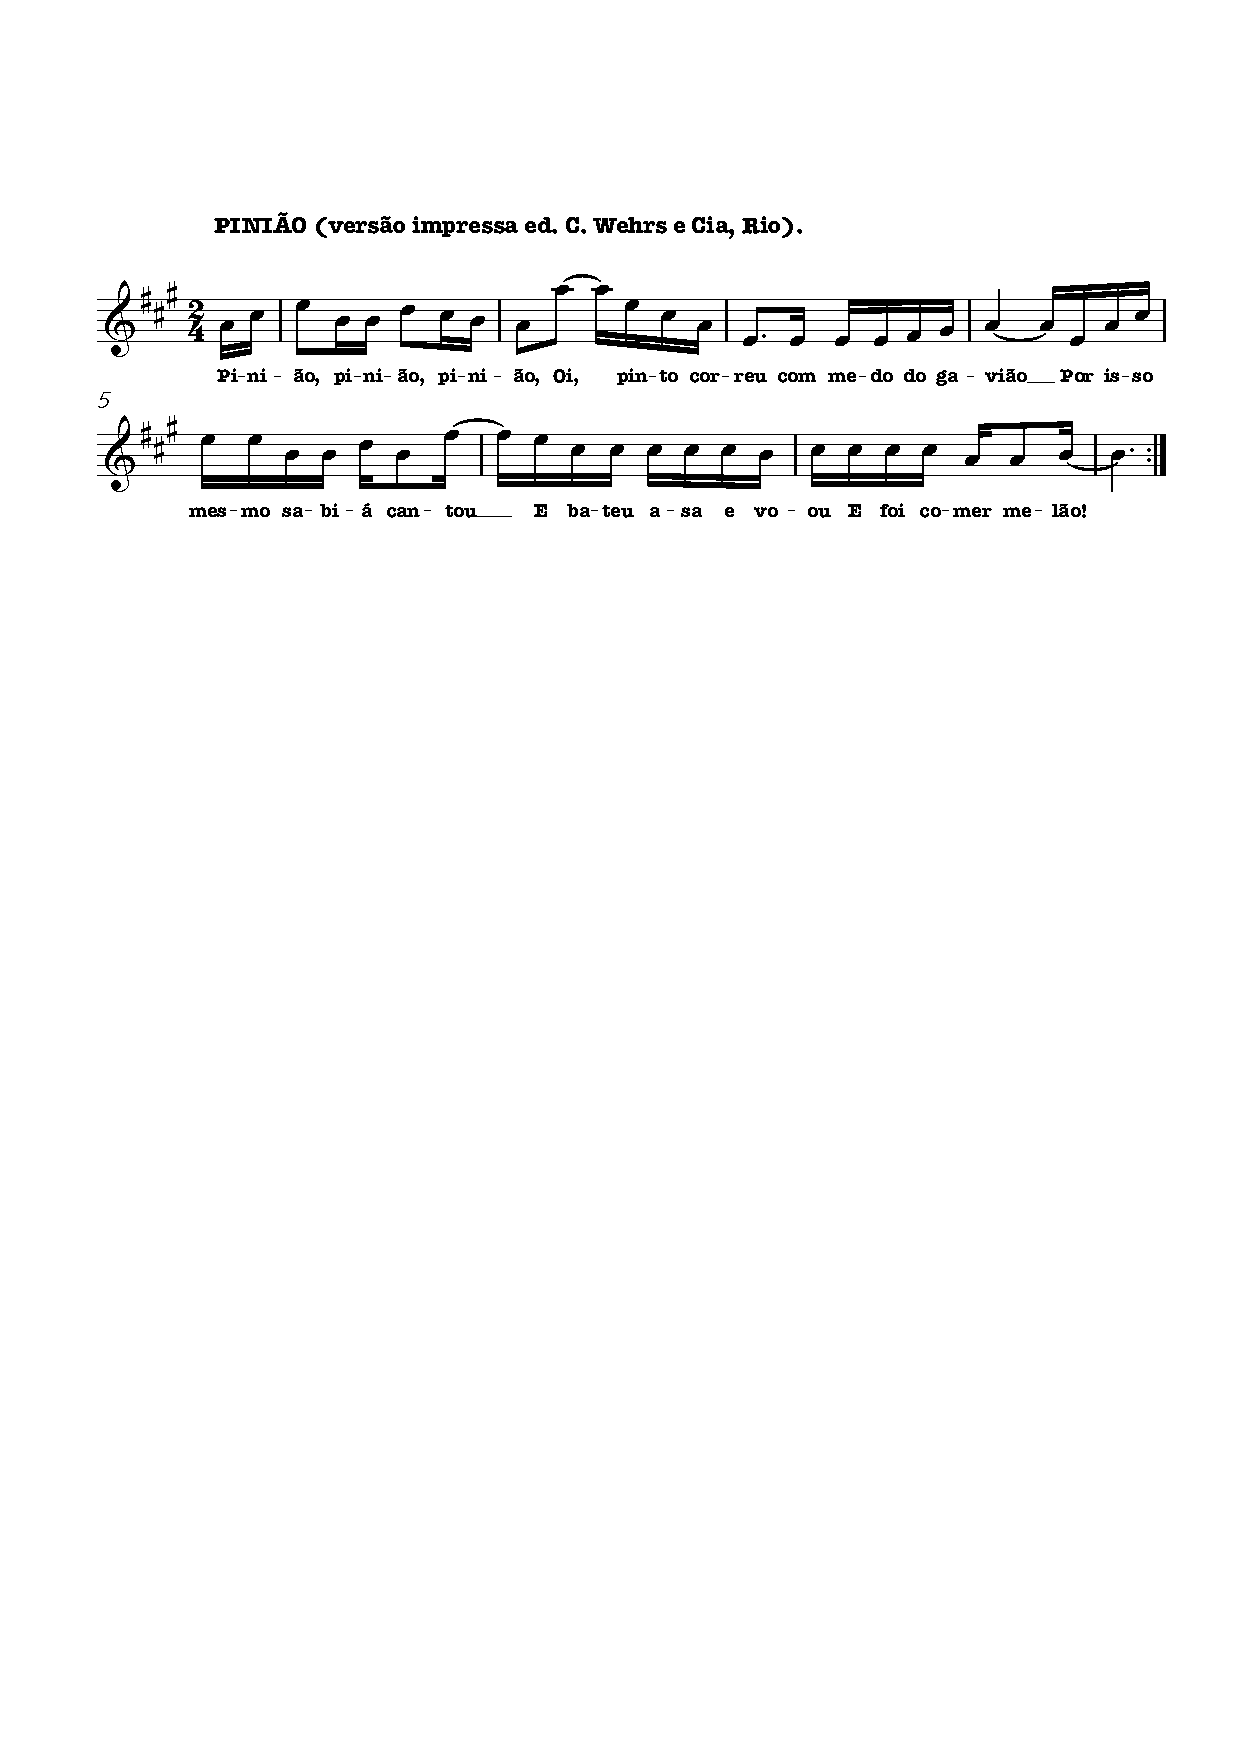
\includegraphics[width=\textwidth]{./imgs/fig1.pdf}
 \end{figure}

\begin{quote}
\forceindent{}Pinião, pinião, pinião,

Oi pinto correu com medo do gavião

Por isso mesmo sabiá cantou

E bateu asa e voou

E foi comer melão!
\end{quote}

 \begin{figure}[H]
 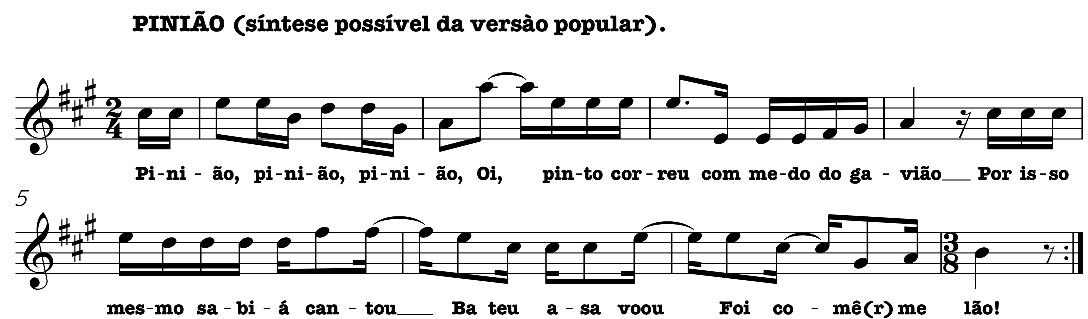
\includegraphics[width=\textwidth]{./imgs/fig2.pdf}
 \end{figure}

\begin{quote}
\forceindent{}Pinião, pinião, pinião,

Oi, pinto correu com medo do gavião

Por isso mesmo sabiá cantou

Bateu asa voou

Foi comê(r) melão!
\end{quote}

 \begin{figure}[H]
 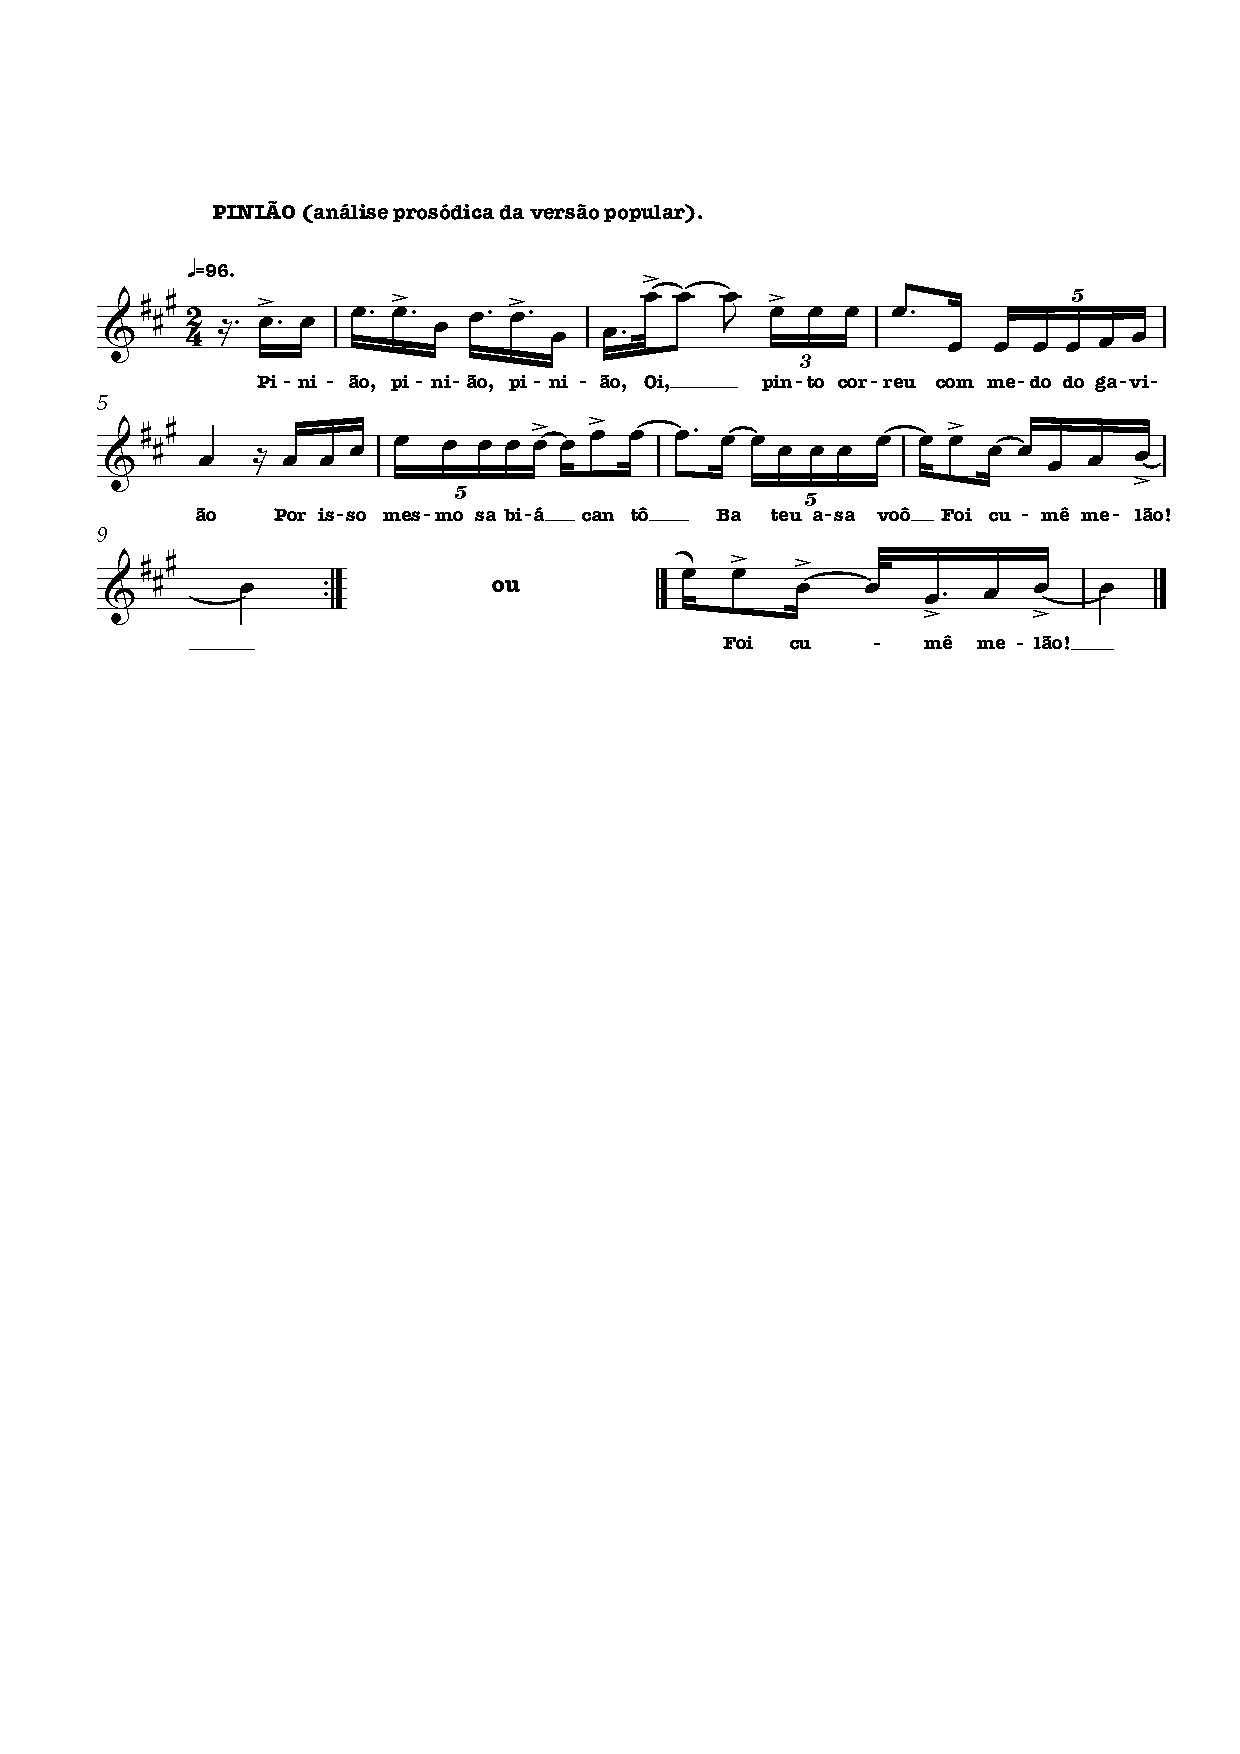
\includegraphics[width=\textwidth]{./imgs/fig3.pdf}
 \end{figure}

Aliás a terceira grafia que indiquei como prosódica pode ser atacada por
isso. De fato qualquer cantiga está sujeita a um tal ou qual \textit{ad
libitum} rítmico devido às próprias condições da dicção. Porém essas
fatalidades da dicção relativamente à música europeia são de deveras
\textit{fatalidades}, não têm valor específico pra invenção nem efeito da
peça. Também muito documento brasileiro é assim, principalmente os do
centro mineiro-paulista e os da zona tapuia. Não falo dos
sul-rio-grandenses porque ainda não escutei nenhum cantador gaúcho, não
sei. Mas o mesmo não se dá com as danças cariocas e grande número de
peças nordestinas. Porque nestas zonas os cantadores se aproveitando dos
valores prosódicos da fala brasileira tiram dela elementos específicos
essenciais e imprescindíveis de ritmo musical. E de melodia também. Os
maxixes impressos de Sinhô são no geral banalidades melódicas.
Executados, são peças soberbas, a melodia se transfigurando ao ritmo
novo. E quanto à peça nordestina ela se apresenta muitas feitas com uma
rítmica tão sutil que se torna quase impossível grafar toda a realidade
dela. Principalmente porque não é apenas prosódica. Os nordestinos se
utilizam no canto de um \textit{laisser aller} contínuo, de feitos
surpreendentes e muitíssimas vezes de natureza exclusivamente musical.
Nada tem de prosódico. É pura fantasia duma largueza às vezes
\textit{malinconica}, ás vezes cômica, ás vezes ardente, sem aquela \textit{tristurinha}
paciente que aparece na zona caipira.

Porém afirmando a grandeza do Nordeste musical não desconheço o valor
das outras zonas. Alguns dos cantos tapuios, os fandangos paulistas de
beira mar, os cantos gaúchos isentos de qualquer hispano americanismo,
expostos na segunda parte deste livro mostram os acasos de ensinamento e
boniteza que deve reservar uma exploração detalhada do populário.

Pelo menos duas lições macotas a segunda parte deste livro dá pra gente:
o caráter nacional generalizado e a destruição do preconceito da
sincopa.

Por mais distintos que sejam os documentos regionais, eles manifestam
aquele imperativo ético pelo qual são facilmente reconhecidos por nós.
Isso me comove bem. Além de possuírem pois a originalidade que os
diferencia dos estranhos, possuem a totalidade racial e são todos
patrícios. A música popular brasileira é a mais completa, mais
totalmente nacional, mais forte criação da nossa raça até agora.

Pois é com a observação inteligente do populário e aproveitamento dele
que a música artística se desenvolverá. Mas o artista que se mete num
trabalho desses carece alargar as ideias estéticas senão a obra dele
será ineficaz ou até prejudicial. Nada pior que um preconceito. Nada
melhor que um preconceito. Tudo depende da eficácia do preconceito.

Cabe lembrar mais uma vez aqui do que é feita a música brasileira.
Embora chegada no povo a uma expressão original e étnica, ela provém de
fontes estranhas: a ameríndia em porcentagem pequena; a africana em
porcentagem bem maior; a portuguesa em porcentagem vasta. Além disso a
influência espanhola, sobretudo a hispano-americana do atlântico (Cuba e
Montevideo, habanera e tango) foi muito importante. A influência
europeia também, não só é principalmente pelas danças (valsa polca
mazurca shottsh) como na formação da modinha.\footnote{Álbum de música nas ``Reise in Brazilien'', Spix e Martius; a peça registrada por Langardorff na ``Viagem ao redor do mundo''; as peças sobre Marília de Dirceu no ``Cancioneiro Portugues'' de César das Neves e Gualdino de Campos (vols.\,19, 21, 29, 32, 44, 47 e 50); ed.\,César Campos e Cia. Porto); modinhas do padre Maurício e outros no ``Cancioneiro Fluminense'' de Mello Morais, etc.} De primeiro, a modinha de
salão foi apenas uma acomodação mais aguada da melodia da segunda metade
do século \textsc{xviii} europeu. Isso continuou até bem tarde como demostram
certas peças populares de Carlos Gomes e principalmente Francisca
Gonzaga.

Além dessas influências já digeridas temos que contar as atuais.
Principalmente as americanas do jazz e do tango argentino. Os processos
do jazz estão se infiltrando no maxixe. Em recorte infelizmente não sei
de que jornal guardo um samba macumbeiro, \textit{Aruê de Changô} de João
da Gente que é documento curioso por isso. E tanto mais curioso que os
processos polifônicos e rítmicos de jazz que estão nele não prejudicam
em nada o caráter da peça. É um maxixe legítimo. De certos os
antepassados coincidem.

Bem mais deplorável é a expansão da melodia chorona do tango. E
infelizmente não é só em tangos argentinos\ldots{} de brasileiros que ela se
manifesta. Tem uma influência evidente do tango em certos compositores
que pretendem estar criando a\ldots{} canção brasileira! Estão nada. Se
aproveitam da facilidade melódica pra andarem por aí \textit{tangaicamente}
gemendo sexualidades panemas.

Está claro que o artista deve selecionar a documentação que vai lhe
servir de estudo ou de base. Mas por outro lado não deve cair num
exclusivismo reacionário que é pelo menos inútil. A reação contra o que
é estrangeiro deve ser feita \textit{espertalhonamente} pela deformação e
adaptação dele. Não pela repulsa.

Se de fato o que já é caracteristicamente brasileiro deve nos interessar
mais, se é preconceito útil preferir sempre o que temos de mais
característico: é preconceito prejudicial repudiar como estrangeiro o
documento não apresentando um grau objetivamente reconhecível de
brasilidade. A marchinha central dos admiráveis ``Choros n.\,5''\footnote{\textit{Alma Brasileira}, Ed. Vieira Machado, Rio.} de
Villa-Lobos foi criticada por
não ser brasileira. Quero só saber por quê. O artista se utilizou dum
ritmo e dum tema comuns, desenvolvidos dum elemento anterior da peça,
tema sem caráter imediatamente étnico nenhum, tanto podendo ser
brasileiro como turco ou francês.

Não vai em nada contra a musicalidade nacional. Portanto é também
brasileiro não só por que o pode ser como por que sendo inventado por
brasileiro dentro de peça de caráter nacional e não levando a música pra
nenhuma outra raça, é necessariamente brasileiro.

E nisto que eu queria chegar: o artista não deve ser nem exclusivista
nem unilateral.

Se a gente aceita como um brasileiro só o excessivo característico, cai
num exotismo que é \textit{exótico até pra nós}. O que faz a riqueza das
principais escolas europeias é justamente um caráter nacional
incontestável, mas na maioria dos casos indefinível, porém. Todo o
caráter excessivo e que por ser excessivo é objetivo e exterior em vez
de psicológico, é perigoso. Fatiga e se torna facilmente banal. É uma
pobreza. É o caso de Grieg e do próprio Albeniz que já fatiga
regularmente. A obra polifônica de Vittoria é bem espanhola sem ter nada
de espanholismo. E felizmente pra Espanha que os trabalhos de Pedrell e
autores como Joaquim Nin, Halfter, Falla estão alargando as
possibilidades do \textit{tatatá} rítmico espanhol.

O exclusivista brasileiro só mostra que é ignorante do fato nacional. O
que carece é afeiçoar os elementos estranhos ou vagos que nem fizeram
Levy com o ritmo de habanera do ``Tango Brasileiro'' ou Villa-Lobos com a
marchinha dos ``Choros n.\,5'' pra que se tornem nacionais dentro da
manifestação nacional. Também se a parte central da ``Berceuse da
Saudade'' de Lorenzo Fernandez constituísse uma
obra isolada não tinha por onde senti-la brasileiramente. Porém essa
parte se torna necessariamente brasileira por causa do que a cerca.
%(op. 55 Ed Bevilaqua)

Mas o característico excessivo é defeituoso apenas quando virado em
norma única de criação ou crítica. Ele faz parte dos elementos úteis e
até, na fase em que estamos, deve de entrar com frequência. ``Porque
é por meio dele que a gente poderá com mais firmeza e rapidez determinar
e normalizar os caráteres étnicos permanentes da musicalidade
brasileira.''

Outro perigo tamanho como o exclusivismo é unilateralidade. Já escutei
de artista nacional que a nossa música \textit{tem de ser tirada dos
índios}. Outros embirrando com guarani afirmam que a verdadeira música
nacional é\ldots{} a africana. O mais engraçado é que o maior número
manifesta antipatia por Portugal. Na verdade, a música portuguesa é
ignorada aqui. Conhecemos um atalho de pecinhas \textit{assim-assim} e conhecemos
por demais o fado \textit{gelatinento} de Coimbra. Nada a gente sabe de Marcos
Portugal, pouquíssimo de Rui Coelho e nada do populário portuga, no
entanto bem puro e bom.

Mas por ignorância ou não, qualquer reação contra Portugal me parece
perfeitamente boba. Nós não temos que reagir contra Portugal, temos é de
não nos importarmos com ele. Não tem o mínimo desrespeito nesta frase
minha. É uma verificação de ordem estética. Se a manifestação brasileira
diverge da portuguesa muito que bem, se coincide, se é influência, a
gente deve aceitar a coincidência e reconhecer a influência. A qual é e
não podia deixar de ser enorme. E reagir contra isso endeusando boróro
ou bantu é cair num unilateralismo tão antibrasileiro como a lírica de
Glauco Velasquez. E aliás, é pela ponte lusitana que a nossa
musicalidade se tradicionaliza e justifica na cultura europeia. Isso é
um bem vasto. É o que evita que a música brasileira se resuma a
curiosidade esporádica e exótica do tamelang javanês, do canto achanti,
e outros atrativos deliciosos, mas passageiros de exposição universal.

O que a gente deve mais é aproveitar todos os elementos que concorrem pra
formação permanente da nossa musicalidade étnica. Os elementos
ameríndios servem sim porque existe no brasileiro uma porcentagem forte
de sangue guarani. E o documento ameríndio propriedade nossa, mancha
agradavelmente de estranheza e de encanto soturno a música da gente. Os
elementos africanos servem francamente se colhidos no Brasil porque já
estão afeiçoados à entidade nacional. Os elementos onde a gente percebe
uma tal ou qual influência portuguesa servem da mesma forma.

O compositor brasileiro tem de se basear quer como documentação que como
inspiração no folclore. Este, em muitas manifestações
\textit{caracteristiquíssimo}, demonstra as fontes donde nasceu. O compositor por
isso não pode ser nem exclusivista nem unilateral. Se exclusivista se
arrisca a fazer da obra dele um fenômeno falso e falsificador. E
sobretudo facilmente fatigante. Se unilateral, o artista vira
antinacional: faz música ameríndia, africana, portuga ou europeia. Não
faz música brasileira não.\footnote{\textls[-10]{No texto original, seguia-se a seção ``Ritmo'', suprimida da presente edição. \textsc{{[}n.\,o.{]}}}}

\section{Melodia}

O problema importante aqui é o da invenção melódica expressiva. O
compositor se vê diante dum dilema. (Pelo menos este dilema já me foi
proposto por dois compositores). É este: o emprego da melódica popular
ou invenção de temas pastichando ela, fazem o autor empobrecer a
expressão. Isso principalmente na música de canto em que o compositor
devia de respeitar musicalmente o que as palavras contam. Os grandes
gênios desde o início da Polifonia vêm pelejando pra tornar a música
psicologicamente expressiva. Todos os tesouros de expressão musical que
nos deram Lasso, Monteverdi, Carissimi, Gluck, Beethoven, Schumann,
Wagner, Wolff, Mussorgsky, Debussy, Strauss, Pizzetti, Honegger etc.
etc. que se confinaram mais pro lado da expressão musical psicológica,
têm que ser abandonados pelo artista brasileiro pra que ele possa fazer
música nacional. Ou o compositor faz música nacional e falsifica ou
abandona a força expressiva que possui, ou aceita esta e abandona a
característica nacional.

Vamos a ver os aspetos mais importantes da questão:

\smallskip
\textit{A música popular é psicologicamente inexpressiva?}
\smallskip

À primeira vista parece. Mas parece justamente porque é a mais
sabiamente expressiva de todas as músicas. O problema da expressão
musical é vasto por demais pra ser discutido aqui. Parece mais acertado
afirmar que a música não possui nenhuma força direta pra ser
psicologicamente expressiva.

A gente registra os sentimentos por meio de palavras. As artes da
palavra são pois as psicológicas por excelência. E como os sentimentos
se refletem no gesto ou determinam os atos as artes do espaço pelo
desenho e pela mimésis coreográfica podem também expressar a psicologia
com certa verdade. Tomo \textit{expressar} no sentido de \textit{contar}, qual é a
psicologia sem que ela seja sabida de antemão.

Pois a música não pode fazer isso. Não possui nem o valor intelectual
direto da palavra nem o valor objetivo direto do gesto. Os valores dela
são diretamente dinamogênicos e só. Valores que criam dentro do corpo
estados sinestésicos novos. Estas sinestesias sendo provocadas por um
elemento exterior (a música) que é recebido por uma determinação da
vontade (pois a gente quis escutar a música) são observadas com acuidade
particular e interesse pela consciência. E a consciência tirar delas uma
porção de conclusões intelectuais que as palavras batizam. Estas
conclusões só serão exatas se forem conclusões fisiológicas. Está certo
falar que uma música é bonita ou feia porque certos estados cenestésicos
agradam ou desagradam sem possuírem interesse prático imediato (fome,
sede \textit{etc}). O \textit{agradável sem interesse imediato} é batizado com o nome de
\textit{Belo}. O desagradável com o nome de \textit{Feio}.

Ainda estará certo a gente chamar uma música de molenga, violenta,
cômoda porque certas dinamogenias fisiológicas amolecem o organismo,
regulariza o movimento dele ou o impulsionam. Estas dinamogenias nos
levam pra estados psicológicos equiparáveis a outros que já tivemos na
vida. Isto nos permite chamar um trecho musical de tristonho, gracioso,
elegante, apaixonado \textit{etc. etc.} Já com muito de metáfora e bastante de
convenção. Só até aí chegam as verificações de ordem fisiopsíquica.

Mas a música possui um poder dinamogênico, muito intenso e, por causa
dele, fortifica e acentua \textit{estados-de-alma} sabidos de antemão. E
como as dinamogenias dela não tem significado intelectual, são
misteriosas, o poder sugestivo da música é formidável.

Ora o que que a música popular faz desses valores e poderes? É sempre
fortemente dinamogênica. É de dinamogenia sempre agradável porque
resulta diretamente, sem nenhuma erudição falsificadora, sem nenhum
individualismo exclusivista, de necessidades gerais humanas
inconscientes. E é sempre expressiva porque nasce de necessidades
essenciais, por assim dizer interessadas do ser e vai sendo
gradativamente despojada das arestas individualistas dela a medida que
se torna de todos e anônima. E como o povo é inconsciente, é fatalizado,
não pode errar e por isso não confunde umas artes com as outras, a
música popular jamais não é a expressão das palavras. Nasce sempre de
estados fisiopsíquicos gerais de que apenas também as palavras
nascem. E por isso em vez de ser expressiva momento por momento, a
música popular cria ambientes gerais, cientificamente exatos,
resultantes fisiológicas da graça ou da comodidade, da alegria ou da
tristura.

É isso que o compositor tem de fazer também.

É impossível pra música expressar (contar) o verso:

\begin{verse}
\small{Tanto era bela no seu rosto a morte.}
\end{verse}

Mas ela pode criar uma cenestesia relativa ao passo do Uruguai.
Ambientar musicalmente o ouvinte de forma a permitir pela sugestão da
dinamogenia uma perceptibilidade mais vivida, mais geral, mais
fisiopsíquica do poema.

Pois esta ambientação não implica liberdade individual nem muito menos
ausência de caráter étnico. Não só dentro de regras e fórmulas estreitas
os gênios souberam ambientar os poemas que musicaram, como nenhum deles
depois que a música se particularizou em escolas nacionais, deixou de
ser nacional. O dilema em que se sentem os compositores brasileiros vem
duma falha de cultura, de uma fatalidade de educação e de uma ignorância
estética. A falha de cultura consiste na desproporção de interesse que
temos pela coisa estrangeira e pela coisa nacional. Essa desproporção
nos permite sentir na permanência do nosso ser mediocridades como
Leoncavallo, Massenet ou Max Reger ao passo que uma voz de congo ou de
catira é um acaso dentro de nós.\footnote{O problema da Sinceridade em arte eu já discuti uma feita em artiguete de jornal (\textit{Diário Nacional}, ``Ângelo Guido'', São Paulo, 10 de novembro de 1927). Confesso que eu considero perfeitamente desimportante. Mas o artista afeiçoado pela tradição e cultura (que não dependeram da folha dele e vem dos professores e do ramerrão didático) adquiriu um jeito natural de escrever e de compor. E depois não quer mudar esse jeito porque é sincero\ldots{} Isso é bobagem. A sinceridade em arte já principia por ser um problema discutibilíssimo, porém mesmo que não fosse, o nosso caso continua desimportante.
Além da sinceridade do jeito existe inteligência que atinge convicções novas. Além da sinceridade do hábito existe a sinceridade intelectual. Desde que a gente chega a uma convicção nova, dá um exemplo nobre de sinceridade, contrariando o hábito, o jeito já adquirido para respeitar a convicção nova. O indivíduo que está convicto de que o Brasil pode e deve ter música própria, deve de seguir essa convicção, muito embora ela contrarie aquele habito antigo pelo qual o indivíduo inventava temas de músicas via Leoncavallo-Macenet-Reger. E isso nem é tão difícil como parece. Com poucos anos de trabalho literário de alguns os poetas novos aparecendo trazem agora um cunho inconfundível de Brasil na poesia deles. Outro dia um músico ainda estudante me falava na dificuldade vasta que sentia em continuar o estudo da Fuga por ter escrito umas poucas obras brasileiras ``já se acostumaram tanto que tudo lhe saía brasileiro da invenção''. Nos países em que a cultura aparece de emprestado que nem os americanos, tanto os indivíduos como a arte nacionalizada, têm de passar por três fases: 1ª a fase da ``tese'' nacional; 2ª a fase do ``sentimento'' nacional; 3ª a fase da ``inconsciência'' nacional. Só nesta última Arte culta e o indivíduo culto sentem a sinceridade do hábito e a sinceridade da convicção coincidirem. Não é nosso caso ainda. Muitos de nós já estamos sentindo brasileiramente, não tem dúvida, porém o nosso coração se dispersa, nossa cultura nos atraiçoa, nosso jeito nos enfraquece. Mas é nobilíssimo, demonstra organização, demonstra caráter, o que põe a vontade como sentinela da raça e não deixa entrar o que é prejudicial. É masculino agente se sacrificar por uma coisa prática, verdadeira, de que beneficiarão os que vierem depois.} A fatalidade de
educação consiste no estudo necessário e cotidiano dos grandes gênios e
da cultura europeia. Isso faz com que a gente adquira as normas desta e
os feitos daqueles, E a ignorância estética é que faz a gente imaginar
um dilema que na realidade não existe, é uma simples manifestação de
vaidade individualista.

Mas como não tenho a mínima ideia de rejeitar os direitos de expressão
individual ainda quero esclarecer um bocado o emprego da melódica
popular.

Se de fato o compositor se serve de uma melodia ou de um motivo
folclórico a obra dele deixa de ser \textit{individualistamente} expressiva como
base de inspiração. E fica o mesmo se o compositor deliberadamente a
molda a invenção aos processos populares nacionais. Isso não tem dúvida.
Porém à base de inspiração tem valor mínimo ou nenhum diante da obra
completa. Basta ver certas harmonizações artísticas de cantos populares.
Bela Bartok, Luciano Gallet, Gruenberg, Percy Grainger perseveram nos
seus caráteres individuais, harmonizando coisas alheias.

Até em música de canto o compositor pode e deve se utilizar da melodia
popular. E não só empregar diretamente a melodia integral que nem faz
frequentemente Luciano Gallet como a modificando num ou noutro detalhe
(processo comum em Villa-Lobos), ou ainda empregando frases populares em
melodia própria (L.\,Fernandez na ``Berceuse da Saudade''). Além disso
existem as peculiaridades, as constâncias melódicas nacionais que o
artista pode empregar a todo momento pra nacionalizar a invenção. As
fórmulas melódicas são mais difíceis de especificar que as rítmicas ou
harmônicas não tem dúvida. Mas existem, porém, e não é possível mais
imaginar um compositor que não seja um erudito da arte dele. Afirmar que
empregamos a sincopa ou a sétima abaixada é uma puerilidade. O
compositor deve conhecer quais são as nossas tendências e constâncias
melódicas. Aliás a sétima abaixada é uma tendência brasileira de que
carece matutar mais sobre a extensão. Isso nos leva pro hipofrígio e as
consequências harmônicas derivantes alargam um bocado a obsessão do
tonal moderno. E a riqueza dos modos não para aí não. De certas melodias
de origem africana achadas no Brasil se colhe uma escala hexacordal
desprovida de sensível cujo efeito é interessantíssimo.\footnote{Ver nos Anais do
5° Congresso Brasileiro de Geografia, vol.\,\textsc{i}, as melodias colhidas por
Manuel Quirino.} Este fenômeno é bem frequente. Eduardo Prado no volume
sobre o Brasil na Exposição Internacional de 89\footnote{Editora Delagrave, Paris.} 
registra a observação de um músico francês sobre melodias nossas
desprovidas de sensível. E mesmo neste ensaio vai como exemplo disso a
versão paraibana do ``Mulher rendeira'' em que a sensível é evitada
sistematicamente. A melódica das nossas modinhas principalmente, é
torturadíssima e isso é uma constância. Na cantiga praceana o brasileiro
gosta dos saltos melódicos audaciosos de sétima, de oitava (Francisca
Gonzaga, ``Menina faceira'' no álbum de A.\,Friedenthal) e até de nona que
nem no lundu ``Yayá, você quer morrer'' de Xisto Baía.\footnote{A.\,Friedenthal,
``Stimmen der Völker'' vol.\,6; ``Papel e Tinta'' n.\,1, S.\,Paulo.} Na segunda
parte deste livro é fácil de assustar isso, e Villa-Lobos na ``Modinha''\footnote{Seresta n.\,5, Editora C.\,Artur Napoleão.} mostra também um exemplo cheio de
espírito.

A inquietação da linha melódica aparece até no canto caboclo embora
menos frequentemente. Está no ``Fotorototó''\footnote{L.\,Galiet ``Seis melodias
populares'', Ed. cit.} e no ``Boiadeiro''\footnote{A.\,Levy, ``Rapsódia brasileira'',
Editora L.\,Levy e Irmão.}

Nossa lírica popular demonstra muitas feitas caráter fogueto, serelepe
que não tem parada. As frases corrupiam, no geral em progressões com uma
esperteza adorável. Sem que tenha nenhuma semelhança objetiva, isso nos
evoca a alegria das sonatas e tocatas do século \textsc{xviii} italiano. É lembrar
a ``Galhofeira''\footnote{Editora Bevilaqua, Rio.} de A.\,Nepomuceno.\footnote{A partir daqui, foram suprimidos os últimos nove parágrafos do texto original, além da seção seguinte, ``Polifonia''. \textsc{{[}n.\,o.{]}}}

\section{Instrumentação}

Será que possuímos orquestras típicas? Possuímos, embora elas não sejam
tão características como o jazz, o gamelão, ou os conjuntos havaianos e
mexicanos. Catulo Cearense no ``Braz Macacão'' enumera um conjunto caboclo
assim:

\begin{verse}
\small{
\textit{Rebeca, frauta, pandeiro,}\\
\textit{clarineta, violão,}\\
\textit{Um bandão de cavaquinho,}\\
\textit{Um ofiscreide, um gaitêro}\\
\textit{Que era um cabra mesmo bão,}\\
\textit{Caxambú\ldots{}}}
\end{verse}

Mais pra diante ajunta o reco-reco, o que faz a gente maliciar que a
enumeração foi em parte determinada pelo acaso do metro\ldots{} Porém, é
incontestável que na \textit{orquestrinha} do poeta a gente reconhece a
sonoridade mais constante da instrumentação nacional. Mesmo os
agrupamentos praceanos se aproximam disso bem. Nas \textit{orquestrinhas} dos
fandangos praieiros de S.\,Paulo ocorre com mais frequência o conjunto:
rebeca (violino), viola, pandeiro, adufe, machete. A sanfona que está
influindo bem na melódica da zona mineira, é acompanhada por triângulo
nos fuás de Pernambuco.

O fato da maioria desses instrumentos serem importados não impede que
tenham assumido até como solistas, caráter nacional. O próprio piano
aliás pode ser perfeitamente tratado pelo compositor nacional sem que
isso implique desnacionalização da peça. O violino se acha nas mesmas
condições e está vulgarizadíssimo até nos meios silvestres. Numa fazenda
de zona que permaneceu especificamente caipira, tive ocasião de escutar
uma \textit{orquestrinha} de instrumentos feitos pelos próprios colonos.
Dominavam no solo um violino e um violoncelo\ldots{} bem nacionais. Eram
instrumentos toscos não tem dúvida, mas possuindo uma \textit{timbração} curiosa
meio nasal meio rachada, cujo caráter é fisiologicamente brasileiro.

Não se trata de desafinação com a qual não posso contar aqui, está
claro. Se trata de caráter de sonoridade, de timbre. Ora o timbre
sinfônico da tal de \textit{orquestrinha} coincidia bem, com a sonoridade musical
mais frequente dos solistas e dos conjuntos vocais brasileiros.
Muitíssimo mais tosca e sem refinamento, era em última análise a mesma
sonoridade quente ingênua verde do admirável Orfeão Piracicabano. Quem
escutar com atenção nisso um conjunto coral estrangeiro desses que nos
visitam, russos, italianos, alemães e um conjunto brasileiro põe logo
reparo numa diferença grande de timbre. E essa \textit{timbração} anasalada da
voz e do instrumento brasileiro é natural, é climática de certo, é
fisiológica. Não se trata do\ldots{} efeito tenorista italiano ou da
fatalidade prosódica do francês.

Talvez também em parte pela frequência da cordeona (também chamada no
país de sanfona ou harmônica), das violas, do oficleide, por um fenômeno
perfeitamente aceitável de mimetismo a voz não cultivada do povo se
tenha anasalado e adquirido um número de sons harmônicos que a aproxima
das madeiras. Coisa a que propendia naturalmente pelas nossas condições
climatéricas e pelo sangue ameríndio que assimilamos. O anasalado
emoliente, o rachado discreto é constante na voz brasileira até com
certo cultivo. Estão nos coros maxixeiros dos cariocas. Permanecem muito
acentuadas e originalíssimos na entoação nordestina. Dei com eles um
Sábado de Aleluia no cordão negro do ``Custa mas Vai'' em São João Del Rei.
Tornei a escutá-lo num boi-bumbá em Humaitá, no rio Madeira. E numa
ciranda no alto Solimões.

E é perfeitamente ridículo a gente chamar essa peculiaridade da voz
nacional, de falsa, de feia, só porque não concorda com a claridade
tradicional da \textit{timbração} europeia. Ser diferente não implica feiura.
Tanto mais que o desenvolvimento artístico disso pelo cultivo pode fazer
maravilhas. Da lira de quatro cordas dos rapsodos primitivos a Grécia fez as
15 cordas da cítara. Do santir oriental e do \textit{cimbalom} húngaro que Lenau
ainda cantou, ao piano de agora, que distância através de todas as
variantes de clavicórdios! Da crueza e dos \textit{erres arranhentos} da fala
dele o francês criou uma escola de canto magnífico. Nosso timbre vocal
possui um caráter passível de se aperfeiçoar. No canto nordestino tem um
despropósito de elementos, de maneiras de entoar e de articular,
susceptíveis de desenvolvimento artístico. Sobretudo o ligado peculiar
(também aparecendo na voz dos violeiros do centro) dum \textit{glissando} tão
preguiça que cheguei um tempo a imaginar que os nordestinos empregavam o
quarto-de-tom. Pode-se dizer que empregam sim. Evidentemente não se
trata dum quarto-de-tom com valor de som isolado e teórico, baseado na
divisão do semitom, que nem o posto em jogo faz alguns anos pelas
pesquisas de Alois Haba. Mas o nordestino possui maneiras expressivas de
entoar que não só graduam seccionalmente o semitom por meio do
portamento arrastado da voz, como esta às vezes se apoia positivamente
em emissões cujas vibrações não atingem os graus da escala. São maneiras
expressivas de entoar, originais, caraterísticas e dum encanto
extraordinário. São manifestações nacionais que os nossos compositores
devem de estudar com carinho e das quais, se a gente possuísse
professores de canto com o interesse pela coisa nacional, podia muito
bem sair uma escola de canto não digo nova, mas apresentando
peculiaridades étnicas de valor incontestável. Nacional e artístico.

Mas eu estava falando na divulgação silvestre que o violino já tem entre
nós. É fato. também na minha viagem fecunda pela Amazônia, tive ocasião
por duas feitas de examinar violinos construídos por tapuios que não
conheciam nem Manaus. E ainda nesses a factura produzia uma \textit{timbração}
estranha que acentuava sem repugnar o anasalado próprio do instrumento.
As rebecas de Cananeia também são feitas pela gente de lá.

O importante pro sinfonista nacional não me parece que seja se servir
pois duma orquestra absolutamente típica. Haja vista o caso do jazz. Se
é certo que a influência dele vale bem; se sem ele não podemos imaginar
a existência do octeto, de Stravinsky ou de ``Jonny spielt auf'' da
Krenek: o valor dele como enriquecimento sinfônico me parece pequeno.
Porque o fato dos instrumentos polifônicos de percussão que nem o piano
e o xilofone fazerem parte quase obrigada das obras sinfônicas de agora,
o fato ainda do protagonismo até solista, que a bateria adquire certas
feitas (por ex. no ``Noneto'', de Villa-Lobos) se coincidem com
manifestações e tendências do jazz: são mais uma circunstância de época
que influência afro americana. Não é por causa do jazz que a fase atual
é de predominância rítmica. É porque a fase atual é de predominância
rítmica que o jazz é apreciado tanto. E com efeito, pra citar um caso
só, a ``Sagração da Primavera'' de Stravinsky é anterior a expansão do
jazz na Europa e é já uma peça predominantemente rítmica, com uma
bateria desenvolvida que\ldots{} profetizava o jazz.

O sinfonismo contemporâneo, que não é de nenhuma nacionalidade, é
universal, pode perfeitamente ser brasileiro também. O que não quer
dizer que os nossos compositores devam tratá-lo que nem fizeram Levy,
Nepomuceno e infelizmente ainda fazem alguns novos. ``Porque é
justamente a maneira de tratar o instrumento quer solista quer
concertante que nacionalizará a manifestação instrumental.'' Nossos
sinfonistas devem depor reparo na maneira com que o povo trata os
instrumentos dele e não só aplicá-la pros mesmos instrumentos como
transportá-la pra outros mais viáveis sinfonicamente. Porque se o
artista querendo numa obra orquestral dar um ponteio que nem o usado
pelos violeiros e tocadores de violão, puser na partitura um
\textit{bandão de cavaquinho}, vinte violas e 15 violões, está claro
que será muito difícil pelo menos por enquanto encontrar mesmo nas
cidades mais populosas do país, número de instrumentistas capazes de
arcar com as dificuldades eruditas da coparticipação orquestral. Se é
possível e recomendável que os nossos compositores escrevam peças
pequenas pra canto e viola, pra violão e flauta, pra oficleide caxambú e
piano, \textit{etc. etc.} e mesmo pra conjuntos de câmara mais ou menos típicos,
um número orquestral de instrumentos característicos dificultava
enormemente a execução da peça. Por isso e também pela eficiência de
instrumentos de maior sonoridade, a transposição de processos é justa e
bem recomendável. Aliás é o que está se fazendo com os compositores
contemporâneos que tomei por mestres neste ensaio. E já que toquei nisto
peço desculpa a outros compositores que também trabalham a coisa
nacional por não citar as obras deles. Não cito porque ainda não se
distinguem por uma dedicação ao problema, que tenha eficiência social.

Pois, voltando pro assunto: acho que as possibilidades de transposição
ainda são maiores do que o já feito. Ou menores\ldots{} porque a transposição
pode desvirtuar ou desvalorizar o instrumento. Como é o caso por exemplo
de certas passagens do violino (especialmente os \textit{pizicatos} da
``Sertaneja'') na ``Suíte pra canto e violino'' de Villa-Lobos.\footnote{Editora Max
Eschig} Mas nossos ponteios, nossos refrões instrumentais, nosso
ralhar, nosso toque-rasgado da viola, os processos dos flautistas e dos
violonistas seresteiros, o oficleide que tem pra nós o papel que o
saxofone tem no jazz, \textit{etc. etc.} dão base larga pra transposição e
tratamento orquestral, de câmara ou solista.

Eu tenho sempre combatido os processos técnicos e o critério
instrumental que enfraquecem ou desnaturam os caráteres do instrumento e
o fazem sair pra fora das possibilidades essenciais dele. Porém não me
contradigo que não. Que o violino banque o violão, que a gente procure
fazer do piano um realejo de rua, uma caixinha-de-música ou uma
orquestra são coisas que não me interessam e na maioria das vezes são
coisas de fato detestáveis. Não se trata disso. Depois de Cesar Franck,
de Debussy, de Villa-Lobos não é possível a gente afirmar que os limites
técnicos e estéticos do piano tenham sido fixados por Chopin. Uma
transposição (não falo propriamente de imitação) da técnica e dos
efeitos de um instrumento sobre outro pode até alargar as possibilidades
deste e pode caracterizar nacionalmente a maneira de o conceber. A
influência do belcanto sobre o violino de Paganini é manifesta e a deste
sobre o piano de Liszt. Ernesto Nazareth soube em alguns dos tangos,
dele transpor pro piano os processos \textit{flautísticos} e a técnica do
cavaquinho sem que perdesse por isso o pianístico excelente da obra
dele. Lourenço Fernandez na ``Canção do violeiro''\footnote{Publicado pela editora Bevilaqua.} faz uma
transposição pianística bem feliz do \textit{toque-rasgado}.

Pois em orquestras comuns mas concebidas assim, o instrumento típico
viria a juntar o seu valor sonoro novo e a sua eficiência de
caraterização. Nossos compositores ainda não imaginaram nisso bem. A
própria maneira seccionada, dialogante com que é tratada tantas vezes a
orquestração moderna facilita a introdução nela de instrumentos típicos.
Um instrumentador bom pode numa orquestra tirar muito efeito com uma
sanfona, com a marimba, com duas, quatro violas e outros instrumentos
polifônicos. E mesmo os instrumentos solistas servem, também, está
claro. E podemos criar agrupamentos de bateria completamente nossos.
Possuímos um dilúvio de instrumentos ameríndios e africanos que merecem
estudo mais inteligente da parte dos nossos construtores de instrumentos
e dos nossos compositores. É ocioso enumerar todos aqui, mesmo porque
não posso garantir que a minha colheita já esteja completa. Mas um
estudo do grupo das três flautas parece, (``Rondônia'' Roquette Pinto) ou
das numerosas flautas dos Aparai (``In Düster des brasilianischen
Ur-walds'', F.\,Spciser) por exemplo, é absolutamente recomendável. Tanto
mais que os instrumentos parece não devem ser chamados de flautas, pois
a sonoridade deles por causa do material e da embocadura, na certa que é
diferente. E o \textit{batacotô}, o \textit{checherê} o \textit{ganzá} o \textit{caiguatazú} o \textit{curugú} e
\textit{jararaca} a \textit{inubia} o \textit{adjá afofiê membí membí-chuê membí-tarará agogô
vatapí maracá boré oufuá etc. etc.} podem servir de condimento ocasional
e porventura permanente. A música brasileira o que carece em principal é
do estudo e do amor dos seus músicos.

\section{Forma}

Me falta tratar o problema da forma\ldots{} Aliás nos ficou do passado um
cacoete detestável: o de chamar de \textit{brasileiro} a peça de caráter
nacional. Se um costume desses era explicável nos tempos de Nepomuceno e
Levy, agora já não tem razão de ser não. Nome assim avisa que o
compositor faz uma concessão ao exótico ou pro estrangeiro.\footnote{``Concerto
italiano'' Bach; ``Sinfonia espanhola'' Lalo; ``Suíte brasileira'',
Respighi.}

Quanto ao emprego de certas formas tradicionais não vejo prejuízo nisso
embora não recomende. É uma inutilidade. Hoje essas formas são simples
nomes como João, Arací, não têm valor formalístico mais. Se a gente lê
``Sinfonia'' no cabeçalho duma obra moderna sabe que se trata de trabalho
mais desenvolvido e nada mais. O \textit{allegro-de-sonata} anda bem
desmoralizado.

Mesmo naqueles que ainda procuram seguir o formulário clássico, a
desabusada libertação contemporânea permite construções que
horrorizariam a Stamitz, e ao próprio C.\,Franck talvez. Se observe o
``Trio brasileiro'' de Lourenço Fernandez. Tratando a forma cíclica pela
exposição de quase todos os temas no primeiro tempo o artista fez deste
uma verdadeira conclusão antecipada. A \textit{coda} do \textit{allegro-de-sonata} sobre o
tema do ``Sapo Jururú'' assume no Trio o valor de \textit{cabeça} e não de \textit{coda}: é
o tema predominante. Com a constância dele e a circulação contínua dos
outros temas sucedeu que o Trio apesar de \textit{formalísticamente} tradicional
adquiriu um caráter de parte única de uma unidade indissolúvel em que os
andamentos diferentes são valores expressivos de estados-de-musicalidade
do artista e não mais as partes dum esquema formal obrigatório. Tudo
feito com uma lógica admirável.

Mas os nossos compositores têm demonstrado poder criador bem pequeno a
respeito de forma, não se aproveitando das que o populário apresenta.
Aproveitam-se quando muito de nomes que nem Villa-Lobos. Mas como a tudo
quanto faz, Villa-Lobos imprimiu aos choros, serestas, cirandas, uma
feição individualista excessiva não se utilizando propriamente das
formas populares nem as desenvolvendo. Em todo caso o autor do genial
``Rasga Coração'' emprega com frequência a peça curta em dois movimentos
sem repetição do primeiro. Essa forma, em que estou longe de propor uma
originalidade brasileira\footnote{Ver as ``Tonadas'' de H. Allende, chileno, \textit{Ed.
Senart}, Paris.} é comum em nosso populário. Ocorre nas rodas infantis\footnote{``A
pombinha voou'', ``Padre Francisco'', segunda parte} nas toadas e
frequentemente nos cocos (ver na segunda parte).

O canto nacional apresenta uma variedade formal que sem ser
originalidade dá base vasta pra criação artística de melodia
acompanhada. Possui uma diversidade rica de formas estróficas com ou sem
refrão. Mesmo a melodia infinita encontra soluções formais típicas nos
cocos. É verdade que na segunda parte deste livro dou apenas uma amostra
do que são os cocos. É que reservei a maioria dos documentos
colecionados pra um livro que sairá no ano que vem. Dentre os desafios
muitos se revestem duma forma estrófica tão vaga (segunda parte, os dois
desafios com Mané do Riachão) que são recitativos legítimos. Ainda sob
o ponto de vista da melodia infinita os fandangos paulistas são de
modelo bom. E ainda lembro os martelos, certos lundus muito
africanizados,\footnote{``Ma Malia'' na segunda parte; ``Lundu do escravo'', \textit{Revista de
Antropofagia}.} as parlendas, os pregões, os cantos de trabalho
sem forma estrófica, as rezas das macumbas. Todas essas formas se
utilizando de motivos \textit{rítmico-melódicos} estratificados e circulatórios,
nos levando pro rapsodismo da Antiguidade (Egito, Grécia) e nos
aproximando dos processos \textit{lírico-discursivos} dos sacerdotes indianos e
cantadores ambulantes russos, nos dão elementos formalísticos e
expressivos pra criação da melodia infinita caracteristicamente
nacional.
%, cit. n.\,6.

Também quanto a formas corais possuímos nos reisados e demais danças
dramáticas, e nos cocos muita base de inspiração formal. Nos cocos
então, as formas corais variam esplendidamente.

Ora, eu insisto no valor que o coral pode ter entre nós.

Musicalmente isso é óbvio. Sobretudo com a riqueza moderna em que a voz
pode ser concebida instrumentalmente, como puro valor sonoro. O Orfeão
Piracicabano empregando sílabas convencionais adquire efeitos
interessantes de \textit{pizzicato}, de destacado breve ou evanescente. E em
boca-fechada obtém efeitos duma articulação e fusão harmônica
absolutamente admiráveis. Ainda aqui o exemplo de Villa-Lobos é
primordial. Se aproveitando do cacofonismo aparente das falas ameríndias
e africanas e se inspirando nas emboladas ele trata instrumentalmente a
voz com uma originalidade e eficácia que não encontra exemplo na música
universal.\footnote{``Sertaneja'', ``Noneto'', ``Rasga Coração'', das editoras citadas.}

Mas os nossos compositores deviam de insistir no coral por causa do
valor social que ele pode ter. País de povo desleixado onde o conceito
de Pátria é quase uma quimera a não ser pros que se aproveitam dela;
país onde um movimento mais fraco de progresso já desumaniza os seus
homens na vaidade dos separatismos; país de que a nacionalidade, a
unanimidade psicológica; uniformes e comoventes independeram até agora
dos homens dele que tudo fazem pra desvirtuá-las e estragá-las; o
compositor que saiba ver um bocado além dos desejos de celebridade tem
uma função social neste país. O coro humaniza os indivíduos. Não
acredito que a música adoce os caracteres não. Si nos tempos de
Shakespeare adoçou já não faz isso mais não. Os círculos musicais que
assunto de longe são sacos de gatos. A música não adoça os caracteres,
porém o coro generaliza os sentimentos. A mesma doçura molenga, a mesma
garganta, a mesma malinconica, a mesma ferócia, a mesma sexualidade
peguenta, o mesmo choro de amor rege a criação da música nacional de
norte a sul. Carece que os sergipanos se espantem na doçura de topar com
um verso deles numa toada gaúcha. Carece que a espanholada do baiano se
confraternize com a mesma baianada do goiano. E se a rapaziada que
feriu o assento no pastoreio perceber que na Ronda gaúcha, na toada
de Mato Grosso, no aboio do Ceará, na moda paulista, no desafio do
Piauí, no coco norte-rio-grandense, uma chula do rio Branco, e até no
maxixe carioca, e até numa dança dramática do rio Madeira, lugar de mato
e rio, lugar que não tem gado, persiste a mesma obsessão nacional pelo
boi, persiste o rito do gado fazendo do boi o bicho nacional por
excelência\ldots{} É possível a gente sonhar que o canto em comum pelo menos
conforte uma verdade que nós estamos não enxergando pelo prazer amargoso
de nos entregarmos pro mundo\ldots{}

Quanto à música pura instrumental possuímos numerosas formas
embrionárias. A forma da Variação é muito comum no populario. O que
carece é especificar e desenvolver nossos processos de variação. Ela
ocorre de maneira curiosa nos maxixes e valsas cariocas sobretudo na
maneira de tratar a flauta. O ``Urubu'', sublime quando executado pelo
flautista Pixinguinha, afinal das contas não passa de um tema com
variações. Nos cocos a variação é comum. Por vezes não são os temas
estróficos que variam propriamente, porém se apresentam acrescentados de
parte nova ou com um dos elementos substituídos por outro que nem se
verá nos ``Fandangos da madrugada'' e na versão araraquarense do ``Sapo
Cururu'' (segunda parte). Por vezes as variantes duma peça muito espalhada
assumem o aspecto de verdadeiras variações que nem no caso do ``Canto de
Usina'' e do coco junto dele (segunda parte).

Quanto a danças temos até demais. Se pela expansão grande que teve a
forma coreográfica do maxixe, este, o samba, a embolada, o cateretê, se
confundem na música popular impressa e praceana, isso não se dá nas
danças de tradição oral. Cada uma delas tem a sua coreografia e seu
caráter, embora a gente possa reduzir todas a três ou quatro tipos
coreográficos fundamentais, que nem já fez Jorge M.\,Furt\footnote{``Coreografia
Gauchesca'' Editora Coni, Buenos Aires, 1927} com as danças argentinas.
Carece, pois, que os nossos compositores e folcloristas vão estudar a
fonte popular pra que as danças se distingam melhor no caráter e na
forma.

L.\,Galiet já se aplicou em parte a isso numa série de peças infantis a
quatro mãos, ainda inéditas.

Sambas, maxixes, cocos, chimarritas, catiras, cururus, faxineiras, candomblés,
chibas, baianos, recortadas, mazurcas, valsas, scottish, polcas,\footnote{As formas de importação que cito já tiveram uma caracterização nacional. Não cito o tango argentino e o fox-trote porque não adquiriram caráter nacional ainda aqui: são simples pastichos.}
bendenguês, tucuzís, serranas, além das que possuem uma só
música própria e particularizadas por alguma peculiaridade coreográfica
e intituladas pelo texto que nem ``Quero Mana'',\footnote{No sul de São Paulo, ``Quero Mana'' também é sinônimo de Desafio. Então, não é dançado.}
``Caramujo'' ``Dão-Dão'' ``Manjericão'' ``Benzinho amor'' ``Nha Graciana'' ``Assú''
``Urutágua'' ``Chico'' ``Benção de Deus'' \textit{etc. etc.} Além das dinamogenias
militares, dobrados marchas de carnaval etc. Tudo isso está aí pra ser
estudado e pra inspirar formas artísticas nacionais.

E além de serem formas isoladas fornecem fundo vasto para criação das
suítes de música pura. E se a métrica das nossas danças obedece no geral
a obsessão brasileira da binaridade, os ritmos, os movimentos são
variadíssimos e com eles o caráter também. A forma de suíte (série de
danças) não é patrimônio de povo nenhum. Entre nós ela aparece bem. No
fim dos bailes praceanos, até nos chás dançantes é costume tocarem a
música ``pra acabar'' constituída pela junção de várias danças de forma e
caráter distintos. E se de fato não basta essa brincadeira possivelmente
de importação, não sei, pra justificar a forma de suíte como hábito
nacional, ela ocorre noutras manifestações também. Nas rodas infantis é
comum a piazada ajuntar um canto com outro. Chegam mesmo a fixar suítes
com sucessão obrigatória de peças. Uma das minhas alunas me exemplificou
isso bem com uma roda grande composta de três melodias tradicionais
reunidas e que as crianças da terra dela jamais imaginariam que não
fosse uma roda só. Os cortejos semirreligiosos semicarnavalescos dos
maracatus nordestinos não são mais que uma suíte. Nas cheganças e
reisados a mesma forma é perceptível. O fandango do sul e meio do Brasil
se na maioria das feitas é sinônimo de bailarico, função, assustado
(aliás o próprio baile é uma suíte) muitas vezes é uma peça em forma de
suíte.

A mim me repugnava apenas que suítes nossas fossem chamadas de \textit{suíte
brasileira}. Por que não \textit{fandango}, palavra perfeitamente
nacionalizada? Por que não \textit{maracatu} pra outra de conjunto mais solene?
Por que não \textit{congado} que tantas feitas perde o seu ritual de dança
dramática pra revestir a forma da música pura coreográfica da suíte? Ou
então inventar individualisticamente nomes que nem a ``Suíte 1922'' de
Hindemith, ou a ``Alt Wien'' de Castelnuovo-Tedesco.

Imagine-se por exemplo uma suíte:

\begin{enumerate}
\item\textit{Ponteio} (prelúdio em qualquer métrica ou movimento);
\item\textit{Cateretê} (binário rápido);
\item\textit{Coco} (binário lento), (polifonia coral), (substitutivo de sarabanda);
\item\textit{Moda ou Modinha} (em ternário ou quaternário), substitutivo da ária antiga);
\item\textit{Cururú} (pra utilização de motivo ameríndio), (pode-se imaginar
  uma dança africana pra empregar motivo afro-brasileiro), (sem
  movimento predeterminado);
\item\textit{Dobrado} (ou samba, ou maxixe), (binário rápido ou imponente final).
\end{enumerate}

Suítes assim, dentro da preferência ou inspiração individual, a gente
pode criar numerosíssimas.

E já que estou imaginando em peças grandes, é fácil de evitar as formas
de sonata, tocata etc. Muito desvirtuadas hoje em dia. É seguir o
exemplo de C.\,Franck no ``Prelúdio coral e fuga''. Dentro de criações
dessas, sempre conservando a liberdade individual a gente podia obedecer
a obsessão humana pela construção ternária e seguir o conselho razoável
de diversidade nas partes. ``Ponteio, acalanto e samba''; ``Chimarrita,
aboio e louvação'' \textit{etc. etc.}

E mesmo formas complexas destituídas de caráter coreográfico, de música
pura ou com intenção descritiva ou psicológica, que nem as peças de
Schumann (``Kinderszenen'', ``Carnaval'' etc.), de Debussy (``Iberia''), de
Malipiero (``Rispetti e Stramboti'') e tantos outros. Ora os nossos
reisados, bumbas meu boi, pastoris, sambas-do-matuto, serestas
(serenatas), cirandas se prestam admiravelmente pra isso. Se um
compositor tiver seu bumba meu boi ou o seu choro, isso impede que
outro crie o dele também? E se pode utilizar nessas formas os próprios
temas populares, como estes mudam de lugar pra lugar, de tempo em tempo,
de ano em ano até o quê que impede a utilização nessas formas de temas
inventados pelo próprio compositor? Nada.

Não é na procura de formas características que o artista se achará em
dificuldade. Porém duas coisas se opõem a fixação e generalização de
turmas nacionais: a dificuldade de estudo do elemento popular e o
individualismo bastante ridículo do brasileiro.

Nosso folclore musical não tem sido estudado como merece. Os livros que
existem sobre eles são deficientes sob todos os pontos de vista. E a
preguiça e o egoísmo impede que o compositor vá estudar na fonte as
manifestações populares. Quando muito ele se limita a colher pelo bairro
em que mora o que este lhe faz entrar pelo ouvido da janela.

Quanto à vaidade pessoal se um músico der pra uma forma popular uma
solução artística bem justa e característica, os outros evitarão de se
aproveitar da solução alheia. Nós possuímos um individualismo que não é
libertação: é a mais pífia, a mais protuberante e inculta vaidade. Uma
falta de cultura geral filosófica que normaliza a nossa humanidade e
alargue a nossa compreensão. E uma falta indecorosa de cultura nacional.
Indecorosa.

A falta de cultura nacional nos restringe a um regionalismo rengo que
faz dó. E o que é pior: essa ignorância ajudada por uma cultura
internacional bêbada e pela vaidade, nos dá um conceito do plágio e da
imitação que é sentimentalidade pura. Ninguém não pode concordar,
ninguém não pode coincidir com uma pesquisa de outro e muito menos
aceitá-la pronto: vira para nós um imitador frouxo.\footnote{Um tempo criticaram ridicularisantemente Lourenço Fernandez porque ``plagiara'' na ``Canção Sertaneja'' (ed. Bevilaqua) o acompanhamento da ``Viola'' (Miniaturas, nº2, ed. C. Artur Napoleão) de Villa-Lobos. A entumecência individualista impedia de verem que se os dois compositores se aplicavam a transpor para o piano processos instrumentais populares, haviam de coincidir nalgum ponto. E, sobretudo, ninguém não percebeu que mesmo tento havido aceitação da parte de L. Fernandez, pois que o processo não era invenção livre do autor da ``Viola'' mas transposição de um processo popular, havia largueza culta em Lourenço Fernandez aceitando uma solução alheia e que essa e que essa largueza homenageava o outro autor em vez de diminuí-lo.} Isto se dá mesmo entre literatos, gente que por lidar com letras é
supostamente a mais culta. A mais bêbeda, concordo.

Todas estas constatações dolorosas me fazem matutar que será difícil ou
pelo menos bem lerda a formação da escola musical brasileira. O lema do
modernismo no Brasil foi ``Nada de escola!''\ldots{} Coisa idiota. Como se
o mal estivesse nas escolas e não nos discípulos\ldots{}

A nossa ignorância nos regionaliza ao bairro em que vivemos. Nossa
preguiça impede a formação de espíritos nacionalmente cultos. Nossa
paciência faz a gente aceitar esses regionalismos e esses
individualismos curtos. Nossa vaidade impede a normalização de
processos, formas, orientações. E estamos embebedados pela cultura
europeia, em vez de esclarecidos.

Os nossos defeitos por enquanto são maiores que as nossas qualidades.
Estou convencido que o brasileiro é uma raça admirável. Povo de
imaginação fértil, inteligência razoável; de muita suavidade e
permanência no sentimento; povo alegre no geral, amolegado pela
malinconia tropical; gente boa humana, gente do quarto de hóspede;
gente acessível;\footnote{Bertoni, ``Anales Científicos Paraguayos'', Série \textsc{iii},
n.\,2, 4° de Antropologia, ed. ``Ex Silvis'', Puerto Bertoni, 1924: livro
que devia de ser cartilha pra brasileiro, e de muita matutação quando
fala na fusão das raças aqui.} povo dotado duma resistência prodigiosa
que aguenta a terra dura, o Sol e o clima detestavam que lhe couberam na
fatalidade. Mas os defeitos de nossa gente, rapazes, alguns facilmente
extirpados pela cultura e por uma reação de caráter que não pode tardar
mais, nossos defeitos impedem que as nossas qualidades se manifestem com
eficácia. Por isso que o brasileiro é por enquanto um povo de qualidades
episódicas e de defeitos permanentes.

Mas este ensaio vai acabar menos \textit{amarguento}. O brasileiro é um povo
esplendidamente musical. Nosso populário sonoro honra a nacionalidade. A
transformação dele em música artística não posso dizer que vai mal, não;
vai bem. Figuras fortes e moças que nem Luciano Gallet, Lourenço
Fernandez e Villa-Lobos orgulhavam qualquer país. Dentre os nomes das
gerações anteriores, vazios são ilustres sem condescendência. Carlos
Gomes pode nos orgulhar além dos pedidos da época e nós temos que fazer
justiça a quem está como ele entre os melhores melodistas universais do
século \textsc{xix}. Os mais novos aparecendo agora se mostram na maioria decididos
a seguir a orientação brasileira dos três mestres que me serviram de
documentação neste livro. Dos nossos virtuoses, alguns nobilíssimos, não
honro estes não: me interessam e glorifico principalmente aqueles uns
que não sacrificados ao ramerrão da plateia internacional, guardam
memória dos nossos compositores nos programas deles. A única bereva da
nossa música é o ensino, pessimamente orientado por toda a parte.

É possível se concluir que neste ensaio eu remoí \textit{lugares-comuns}. Faz
tempo que não me preocupo em ser novo. Todos os meus trabalhos jamais
não foram vistos com visão exata porque toda a gente se esforça em ver
em mim um artista. Não sou. A minha obra desde \textit{Paulicea desvairada} é
uma obra interessada, uma obra de ação. Certos problemas que discuto
aqui me foram sugeridos por artistas que se debatiam neles. Outros mais
fáceis entram pra que meu trabalho possa remediar um bocado a invalidez
dos que principiam. E se o escrito não tiver valor nenhum sempre o livro
se valoriza pelos documentos musicais que seguirão agora.


\chapter{Gravação nacional\footnote{Crônica publicada originalmente no Diário Nacional em 10 de maio de 1930, transcrita aqui com ortografia atualizada. Conferir \textit{A música popular brasileira na vitrola de Mario de Andrade}. São Paulo: Sesc, 2004.}}


Alguns clamam contra a produção nacional de discos e, meu Deus, afinal
das contas têm razão. Mas essa razão é o mais ou menos sutil, mais de
ordem filosófica que propriamente objetiva. Uma coisa de que estou
bastante convencido é que o homem é mesmo um ser notabilíssimo, muito
superior ao que parece na realidade. Essa é a razão pela qual podemos
nos ofender com a discagem que sai. A fonografia brasileira, ou pelo
menos realizada no Brasil, não tem apresentado o homem brasileiro na sua
superioridade virtual.

Mas, como se está vendo, o argumento é de ordem perfeitamente universal.
Primeiro: quero saber mas em que ordem de manifestação humana o homem
brasileiro tem se conservado nesse domínio da sua superioridade virtual,
que ele podia ter? Na economia temos sido duma desastrosa bestice apesar
da clarividência dos Murtinhos. Na política, atos dignos de tradição não
sobem talvez a cinco por cento na gesticulação nacional. Na poesia a
porcentagem é pouco maior, ponhamos uns vinte por cento. E pras artes em
geral vinte por cento já é muito.

Porém o que não consola, mas pelo menos explica, essa inferioridade do
homem brasileiro em relação a si mesmo, é que em todos os países do
mundo se passa mais ou menos a mesma coisa. Quais os livros de versos
que se salvam na poetagem francesa, por exemplo? Incontestavelmente uma
ninharia em relação ao todo. De certo os franceses são dos piores poetas
do mundo e escolhi mal exemplo. Peguemos o \textit{jazz}, que está mais
próximo da verdade. Já está mais do que sabido que o \textit{jazz} é um
dos problemas mais complicados da etnografia universal e o melhor é a
gente se ficar pensando que um \textit{jazz} definitivo específico e
histórico não existe. Mas o que me impressiona é que também não existe
ianque profundamente sabido em coisas de \textit{jazz} que não recuse por
não ser produção básica, e não ter a superioridade\ldots{} virtual do
\textit{jazz}, noventa por cento da manifestação que corre como tal, já
não digo no mundo, mas nos norte-americana.

Inda faz pouco afirmava isso mesmo Erwin Schwerke (\textit{Kings Jazz and
David),} acrescentando que mesmo as \textit{orquestrinhas} ianques de negros,
judeus e internacionais que percorrem a terra são apenas \textit{jazz} pra
inglês ver, e nada têm desse legítimo rei do nosso tempo.

De todas essas considerações aparentemente otimistas em relação ao
Brasil, me convenço de outra coisa: estou inabalavelmente convencido de
que o homem é incapaz de ser humano e que na realidade o que ele é, com
perdão da palavra, não digo.

Da discação internacional, escapam do ruim talvez uns trinta por cento.
Está claro que não falo como fabricação, que essa em algumas fábricas,
Brunswick, Victor, Gramphone, a maioria das vezes é esplêndida. Falo da
música que essas mesmas fábricas no dão. E se a crítica de discos
universal não estivesse ainda tanto no domínio dessas gentilezas,
ponhamos, sociais que permitem a um Henry Prunières criticar com a mesma
complacência \textit{Pulcinella} de Stravinki e \textit{E licevan le stelle}\ldots{}, estou
vendo o clamor humano justo, justificadíssimo contra a discoteca
universal.

A discação brasileira é quase que exclusivamente do domínio da música
popular urbana, quero dizer, a depreciada, banalizada pelos males da
cidadania. O favor dum amigo \textit{vitrolófilo} (quanto neologismo!) me tem
proporcionado felizmente a audição desse gênero musical, de vários
países europeus e americanos. Franqueza: a produção é o que tinha de
ser, dada a incapacidade do homem ser humano. E não é inferior à nossa.
Nem superior. O bom, o que mostra o homem na sua superioridade virtual,
continua duma porcentagem mínima. O que temos a fazer, os que
colecionamos Dante, Shakespeare, Shelley, Goethe, Heine e talvez
Baudelaire em nossas bibliotecas, é selecionar também os discos de
valor.

Ultimamente ainda ouvi dois que não podem ficar ausentes duma discoteca
brasileira: o Babaó Miloqué (Victor) e o Guriatã de coqueiro (Odeon).
São duas peças absolutamente admiráveis como originalidade e caráter. E
admiravelmente executadas.

A história do primeiro nos dá uma lição. A primeira registração da
melodia era banal, não escapava da sonoridade normal das \textit{orquestrinhas}
maxixeiras do Rio. Foi recusada por isso. O autor Josué Barros, se viu
na contingência de fazer coisa \textit{nova}. Mas o novo pro indivíduo
folclorizado é muito relativo e as mais das vezes se confina
(felizmente) em desencavar passados que guardou de sua própria vida, ou
lhe deram por tradição. Toda a originalidade do Babó Miloquê está nisso.
Uma orquestração interessantíssima que, excluindo os instrumentos de
sopro, é exatamente, e com menos brutalidade no ruído, a sonoridade de
percussão dos maracatus do Nordeste.

A lição está clara. Exigir do produtor de músicas folclorizado que não
se deixe levar pelo fácil que lhe dá menos trabalho. Guiar os passos
dele pra evitar nos discos (que não são documentação rigidamente
etnográfica) a monotonia que é por exemplo a censura possível a discos
também esplêndidos como \textit{Vamo apanhá limão} (Odeon), \textit{O senhor
do Bonfim} (Vistor), ou o recente \textit{Escoieno noiva} (Colúmbia), da
série regional de Cornélio Pires. A intromissão da voz tem de ser dosada
pra evitar o excesso de repetição estrófica. Os acompanhamentos têm de
variar mais na sua polifonia, já que não é possível na harmonização, que
os tornaria pedantes e extra populares. E variar também na
instrumentação. E que isso é possível dentro do caráter nacional, provam
muito bem os dois lindos discos que citei anteriormente.


\chapter{Carnaval tá aí\footnote{Esta crônica foi escrita em 18 de janeiro de 1931 para o Diário Nacional, transcrita aqui com ortografia atualizada. Publicada no livro \textit{A música popular brasileira na vitrola de Mario de Andrade}.}}

Preocupações, preocupações, comunismo, Instituto do Café, falam os
heróis, mas, mas, carnaval tá aí. Otília Amorim, num samba, com razões
que sem serem propriamente intelectuais, razões de perna, digamos, que
sempre também são razões, filosofa que nem mesmo o dinheiro é que lhe
permite a felicidade que possui\ldots{} Carnaval tá aí, agruras, desocupação
itinerante, álcool motor\ldots{} nada prejudica: o Brasil vai entrando em
estado de felicidade. Já é sabido que o preparo e enfim gozo do carnaval
é uma das causas do nosso conformismo.

Mas o que me interessa no carnaval neste momento é a nossa música que
sempre teve nele uma das fontes fecundas de evolução. O maxixe nasceu do
carnaval, parece quase certo, lá na caverna carioca dos estudantes de
Heidelberg. Nele ainda, a nossa dança cantada principal evolucionou. Ao
contato dos temas melódicos nordestinos se tornou melodicamente mais
pesada, menos irrequieta na rapidez de movimento. E retomou por isso e
com isso o nome de Samba, que hoje é uma variante do maxixe carioca mais
importante que ele, até no próprio Rio de Janeiro.

O carnaval é uma espécie de cio ornitológico do Brasil, o país bota a
boca no mundo numa cantoria sem parada. Vão aparecendo as danças novas,
as marchinhas safadas, os batuques \textit{maracatuzados}. Dantes as cantigas
novas vinham mais penosamente através da música impressa e a propaganda
das \textit{orquestrinhas} de bares, agora não: o lançamento se faz quase
exclusivamente através dos discos de gramofone. São as grandes casas de
fonografia que se incumbem atualmente da fixação e evolução da nossa
dança cantada.

Ora, estes últimos anos os discos de carnaval nada têm produzido de
muitíssimo notável. A \textit{Pavuna} do ano passado era duma mediocridade
desolante. Se não me engano, depois do \textit{Pinião} que do Nordeste
veio, não tivemos mais nada de verdadeiramente bom. Tenho aqui comigo os
discos de carnaval lançados agora pela fábrica Victor, e encontro no
meio deles, entre as mesmas mediocridades de sempre, três discos de
valor artístico e excepcional. Não sei se terão sucesso popular e
ficarão na memória das ruas carnavalescas, o povo é sempre um segredo.
Ora acata o bom, ora o pior, dominado por uma lei secreta que pelo menos
por enquanto ninguém não descobriu. Não posso augurar nada pois, mas
nada impede que sejam estes três discos, das coisas melhores da discagem
popular nacional.

Dois deles representam bem o Rio, o terceiro é todo o Nordeste
carnavalesco: \textit{Nego Bamba} (33413), \textit{Desgraça pouca é bobage}
(33404), e \textit{São Benedito é ôro só} (33380).

Dos dois primeiros, preciso guardar o nome do compositor J.\,Aimberê, que
será talvez o substituto de Sinhô, não sei. Estas obras deles são
curiosíssimas. Pegou bem aquela maneira de seccionar constantemente as
frases do canto, coisa que Sinhô tinha como admirável habilidade e em
que o nosso canto maxixeiro de procedência negra vai coincidir
curiosamente com o processo improvisatório vocal dos blues afro-ianques.
Mas não é apenas pela música que Nego Bamba e Desgraça pouca são
esplêndidos. São na realidade discos perfeitíssimos como riqueza e
caráter orquestral, como escolha de sonoridades vocais e como gravação.
A fábrica Victor tem hesitado e mesmo errado bastante nas suas gravações
brasileiras. Diante de sonoridades novas, de processos novos de cantar,
era natural, os técnicos norte-americanos que vieram para cá se
desnortearam. Muitos foram os insucessos, em principal pela má
disposição de instrumentos, ante o microfone. Especialmente nas cantigas
e danças com viola, só ultimamente, ao cantar do delicioso piracicabano
Zido Dias, é que a fábrica Victor conseguiu algum equilíbrio e discos
bons. Nestes agora a gravação já é perfeita.

E quem merece ainda todos os aplausos é a cantora. Otília Amorim, cuja
voz gasta e admiravelmente expressiva\ldots{} do que se trata, soube tirar
efeitos magníficos, principalmente no Nego Bamba, que, no gênero, é
incontestavelmente uma obra-prima.

A outra obra-prima do terno é o \textit{São Benedito é ôro só}, de Mora da
Mota, sem dúvida aproveitando temas-nordestinos. Que saudades que me
deu, Recife, cair do frevo, ou então, lá \textit{prás} bandas do trem-de-ferro,
sambando com os negros do Leão Coroado, até fugir num último esbafo,
pedindo a bênção pra cachorro e chamando gato de tio\ldots{} O disco é uma
adaptação admirável dos processos musicais de maracatus, conseguindo,
sem descaracterizar nada, tirar os defeitos da manifestação popular, em
principal o excesso desequilibrado da percussão que chega às vezes a
impedir totalmente que se escute a linha da melodia. No disco não, a
introdução discreta dum instrumento de cordas dedilhadas, na percussão é
duma graça deliciosa, o percuciente da voz solista, quase tão excelente
na sua nasalação como o maravilhoso solista do \textit{Vamo apanhá limão},
a bonita cor do segundo plano do coral, tudo concorre pra fazer desse
disco uma das obras-primas da discação nacional.

Qual! Diante de coisas assim a gente perde a tramontana, cai no frevo e
manda à fava todas circunspecções. E tanto mais este ano, em que a
rapidez da desgraça e a oratória dos heróis só tornou mesmo possível a
felicidade de Otília Amorim\ldots{}

\begin{verse}
\small{
--- Tu vais!\\
Mas, e os teus pais?\\
--- É Carnaval!\ldots{}}
\end{verse}


\chapter{A música e a canção populares no Brasil\footnote{Capítulo do livro \textit{Ensaio sobre a música brasileira}, transcrito aqui com ortografia atualizada.}}

O estudo científico da música popular brasileira ainda está por fazer.
Não há sobre ela senão sínteses mais ou menos fáceis, derivadas da
necessidade pedagógica de mostrar aos estudantes a evolução histórica da
música brasileira. Por isso, o que existe de publicado tende
naturalmente a estabelecer generalizações, muito mais de ordem crítica e
práticas sobre origens, influências e possibilidades musicais, deixando
de lado qualquer análise técnica mais profunda, que possa realmente
interessar à musicologia folclórica.

É preciso distinguir, primeiramente, que em nossos países americanos, há
sempre dois campos distintos que a musicologia folclórica deverá
cultivar. Dum lado está a música dos ameríndios, doutro a música popular
nacional propriamente dita.

A música dos ameríndios do Brasil é quase desconhecida em suas criações
melódicas. Jean de Léry já grafava em nosso primeiro século algumas
melodias dos Tupis do litoral, mas tanto dessa como de outras
contribuições de igual gênero, não temos possibilidade alguma de
controle para determinar se são exatas ou não. O mais provável é que
sejam todas inexatas. Só no século \textsc{xx} aparecem estudos feitos sobre a
prática musical dos ameríndios brasileiros, mas são poucos números e
circunscritos a regiões relativamente pequenas.

Quando à música popular nacional, propriamente dita, a bibliografia
também apresenta pequeno número de obras de valor realmente folclórico.
A musicologia nacional está na infância, e só recentemente se vão
fazendo colheitas de melodias, com espírito científico.

Aliás, o problema da música popular brasileira é de natureza muito
especial, pelo fato de sermos uma nacionalidade de formação recente e
não propriamente autóctone. As próprias condições e progressos de feição
americana, transformam poderosamente o processo das nossas
manifestações, populares ou não. Por tudo isso, um conceito rigidamente
científico de \textit{canção popular}, tal como a etnografia a define, nos
levaria com o sr.\,Julien Tiersot, na \textit{Encyclopédia de la Musique de
Lavignac,} a encerrar a possibilidade de negar a existência de canções
populares entre os americanos!

A bem dizer, o Brasil não possui canções populares, muito embora possua,\label{dizer}
incontestavelmente, músicas populares. Quero dizer: nós não temos
melodias tradicionalmente populares. Pelo menos não existem elementos
por onde provar que tal melodia tem sequer um século de existência. Os
pouquíssimos documentos musicais populares impressos que nos ficaram, de
fim do século \textsc{xviii} ou princípios do século seguinte, já não são mais
encontrados na boca do povo, que deles se esqueceu. Existem tantos
populares, principalmente romances e quadras soltas, de origem ibérica,
que permanecem até agora cantados. (E mesmo destes, uma grande figura de
folclorista, como Amadeu Amaral, levado pelo conceito do anonimato
multissecular e generalização popular de Folclore, se viu obrigado a
aceitar apenas em número muito restrito, nos seus estudos). Porém, esses
documentos recebem melodias várias em cada região e mesmo em cada lugar.
Será possível alguma rara vez determinar, pelo estudo dessas diversas
melodias sobre um mesmo texto, que uma parece mais antiga que a outra;
mas é impossível, pela ausência de elementos de confrontação, imaginar o
grau de ancianidade de qualquer delas.

Assim, não teremos o que cientificamente se chamará de \textit{canção
popular}. Mas seria absurdo concluir por isso que não possuímos música
popular! Tanto no campo como na cidade florescem com enorme abundância
canções e danças que apresentam todos os caracteres que a ciência exige
para determinar a validade folclórica duma manifestação. Essas melodias
nascem e morrem com rapidez, é verdade, o povo não as conservas na
memória. Mas se o documento musical em si não é conservado, ele se cria
sempre dentro de certas normas de compor, de certos processos de cantar,
reveste sempre formas determinadas, se manifesta dentro de certas
combinações instrumentais, contém sempre certo número de constâncias
melódicas, motivos rítmicos, tendências tonais, maneiras de cadenciar,
que todos já são tradicionais, já perfeitamente anônimos e autóctones,
às vezes peculiares, e sempre característicos do Brasileiro. Não é tal
canção determinada que é permanente, mas tudo aquilo do que ela é
construída. A melodia em seis ou dez anos poderá obliterar-se na memória
popular, mas os seus elementos constitutivos permanecem usuais no povo,
e com todos os requisitos, aparências e fraquezas do \textit{tradicional}.

Outra face do problema que exige adaptação americana especial, é a
questão do urbano. É de boa ciência afastar-se de qualquer colheita
folclórica a documentação das grandes cidades, quase sempre impura. Será
possível adotar-se semelhante critério ao Brasil?

As condições de rapidez, falta de equilíbrio e de unidade do progresso
americano tornam indelimitáveis espiritualmente, entre nós, as zonas
rural e urbana. Nas regiões mais ricas do Brasil, qualquer \textit{cidadinha} de
fundo sertão já possui água encanada, esgoto, luz elétrica e rádio. Mas,
por outro lado, nas maiores cidades do país, Rio de Janeiro, no Recife,
em Belém, apesar de todo o progresso, internacionalismo e cultura,
encontram-se núcleos legítimos de música popular em que a influência
deletéria do urbanismo não penetra.

A mais importante das razões desse fenômeno está na interpenetração do
rural e do urbano. Com exceção do Rio de Janeiro, de São Paulo, e poucas
mais, todas as cidades brasileiras estão em contato direto e imediato
com a zona rural. Não existem, a bem dizer, zonas intermediárias entre o
urbano e o rural, propriamente ditos. No geral, onde a cidade acaba, o
campo principia. E realmente numerosas cidades brasileiras, apesar de
todo o seu progresso mecânico, são de espírito essencialmente rural.

Por tudo isso, não se deverá desprezar a documentação urbana.
Manifestações há, e muito características, de música popular brasileira,
que são especificamente urbanas, como o choro e a modinha. Será preciso
apenas ao estudioso discernir no folclore urbano, o que é virtualmente
autóctone, o que é tradicionalmente nacional, o que é essencialmente
popular, enfim, do que é popularesco, feito à feição do popular, ou
influenciado pelas modas internacionais.

Recusar a música popular nacional, só por não possuir ela documentos
fixos, como recusar a documentação urbana só por ser urbana, é
desconhecer a realidade brasileira.\footnote{No exemplar consultado para a transcrição, há um traço lateral feito à lápis do parágrafo que começa com \textit{A bem dizer}, na p.\,\pageref{dizer}, até este ponto. A frase ``mas tudo aquilo de que ela é construída'', compreendida nesse trecho, foi grifada a lápis. De acordo com os métodos de trabalho de Mário de Andrade, esses traços seriam marcas para fichamento, estudo mais desenvolvido ou
aproveitamento em outra obra. A partir daqui, foram suprimidas quatro seções do texto original. \textsc{{[}n.\,o.{]}}}

\chapter{A pronúncia cantada e o problema do nasal brasileiro através dos discos\footnote{Este trabalho foi apresentado por Mário de Andrade no 1º Congresso da Língua Nacional Cantada, de 1937, e discute dicção entre cantores e cantoras do \textit{bel canto}. Foi depois publicado como um capítulo do \textit{Aspectos da música brasileira}, volume \textsc{xi} de suas Obras Completas. Cf. \textit{Aspectos da Música Brasileira}, organização de 2012 da Nova Fronteira.}}

Num dos seus ``Ensaios de antropologia brasiliana'',\footnote{E. Roquette-Pinto: \textit{Ensaios de anthropologia brasiliana} in Biblioteca Pedagógica Brasileira -- Comp. Editora Nacional, São Paulo, 1933 (p.\,97).} o sr.\,Roquette-Pinto
principia afirmando que ``há, pelo menos, uma diferença essencial entre
os idiomas falados oficialmente em Portugal e no Brasil: a pronúncia. É
fato evidente, que ninguém contesta.''

Ninguém o contesta, com efeito, e não teremos jamais precisão de
laboratórios de fonética experimental para verificar tão nua verdade.
Permite-se, no entanto, a Discoteca Pública de São Paulo, no início
desta sua comunicação ao Congresso da Língua Nacional Cantada, exprimir
o voto insistente para que se montem no Brasil, o mais breve possível,
alguns laboratórios de fonética experimental. Só com eles, em comparação
com o que já se tem feito em Portugal, poderemos chegar a uma
consciência científica das profundas dissemelhanças do nosso falar em
relação ao português, bem como das variantes que já começam a se fixar
nitidamente nas pronúncias regionais do Brasil.

A fala dum povo é porventura, mais que a própria linguagem, a melhor
característica, a mais íntima realidade se não da sua maneira de pensar,
pelo menos da sua maneira de expressão verbal. É a luta perene entre o
chamado \textit{erro de gramática} e a verdade. No papel um pronome poderá
estar mal colocado, na fala nunca. As próprias deficiências de expressão
verbal da gente iletrada, são mais que discutíveis. Elas não derivam da
ignorância gramatical ou vocabular, mas afundam as suas raízes num
estádio psíquico diverso que as justifica e lhes tira totalmente o
caráter de \textit{deficiências}. E de resto estão condicionadas a mil outras
maneiras de expressão, o gesto, o rosto, a entoação, e um mesmo
silêncio, muito mais ricos de vida, e suficientemente sintéticos para
substituírem a abundância de vocabulário e a ideia clara das
literaturas.

A língua realmente viva, a que vive pela boca e é irredutível a sinais
convencionais, é o que dá o sentido expressional duma nacionalidade.

\begin{quote}% Por que small?
\small{Mais que o significado especial das palavras, a entoação geral do
idioma, a acentuação e o modo de pronunciar os vocábulos, o timbre das
vozes é que representam os elementos específicos da língua de cada povo.
Essa música racial da linguagem corresponde, em harmonia perfeita, aos
outros caracteres da raça, e é tão verdadeiro este fato que as canções,
quando traduzidas de uma para outra língua, perdem grande parte do seu
encanto.}\footnote{E. Dupré e M. Nathan: \textit{Le Langage Musical} (n.\,607). Ed. Felix Alcan-Paris, 1911 (p.\,27).}
\end{quote}

Mas se não possuímos ainda os laboratórios de fonética experimental que
nos venham dar uma certeza científica sobre a nossa exata pronúncia, é
certo que a discoteca brasileira já nos fornece material abundante de
observação e de exemplo, muito mais útil, muito mais normativo
principalmente que a observação escrita e os sinais da grafia musical.
Não só a pronúncia oral tem seus caracteres especiais, mas essa mesma
pronúncia, quando cantada, se transforma, ou melhor, se condiciona aos
caracteres da voz musical, resultando desse mútuo condicionamento de
palavra e canto, a beleza exata e a total validade expressiva das
músicas nacionais. Nunca uma canção transcrita no papel ou no
instrumento poderá dar a quem a estuda, a sua exata realidade. E a
verificação desta verdade, depois que a fonografia veio nos apresentar o
mundo de riqueza do cantar de todos os povos da Terra, tornou a grafia
musical por meios não mecânicos, bastante desautorizada como base de
estudos etnográficos e folclóricos. Na sua admirável monografia sobre a
música negro-africana, o professor Hornbostel afirmava preliminarmente
que ``como material para estudo, os fonogramas são imensamente
superiores à notação das melodias e não se pode conceber que este método
inferior ainda seja usado. Basta verificar que exclusivamente por meio
da fonografia, é que podemos obter a coisa legítima. O pressuposto geral
de que a substância de uma canção pode ser notada em pauta com os
auxílios, talvez, de sinais diacríticos e texto explicativo, é mera
superstição europeia, ocasionada pela evolução da música e a maneira
geral de pensar dos europeus. Os próprios cantores dão tanta importância
ao timbre da voz e à dicção como a qualquer outra coisa. E mesmo às
vezes mais. De fato, dicção e timbre demonstram ser caracteres raciais
profundamente predeterminados por funções fisiológicas, e são, por isso,
valiosa prova das relações e diferenciações antropológicas. Assim, os
povos e suas músicas, não se distinguem tanto pelo que cantam como pela
maneira porque cantam. Que pensaríamos dum estudante de filologia que se
despreocupasse da fonética? E como poderá ninguém estudar foneticamente
uma língua sem tê-la ouvido falar?''.\footnote{E.M. Hornbostel: \textit{African Negro Music}. Ed. International Institute of African Languages and Cultures -- Londres (p.\,5).}

Estas justas apreciações do célebre etnógrafo sobre o valor da
fonografia vêm de encontro a um problema do canto nacional que a
Discoteca Pública ousa considerar de máxima importância para a música
erudita do Brasil: o problema do \textit{bel canto}.

O \textit{bel canto}, ou mais exatamente as diversas escolas do canto europeu,
tem sido até agora a única base de estudos, a única fonte de exemplos, a
única lei de conduta do canto erudito nacional. Ora, estribada em tão
ilustres professores como os que já citamos, ousa a Discoteca Pública
perguntar se tal orientação é acertada? Si realmente pretendemos
nacionalizar a nossa música erudita, trabalho em que coincidem
atualmente os poderes públicos, os institutos musicais e quase todos os
compositores do país, não seria também justo que os nossos cantores e
professores buscassem também nacionalizar o nosso canto, indo beber na
fonte do povo o mesmo alimento fecundo em que os nossos compositores se
reforçam? Ninguém duvida que o \textit{bel canto} europeu, o \textit{bel canto} que é um
só, possa prover o canto nacional brasileiro dos mesmos estudos técnicos
de desenvolvimento vocal que tanto servem a um alemão como a um
português. E isso mesmo, porque o canto nacional brasileiro tem as
mesmas bases tonais e harmônicas do canto europeu e dele se criou.
Podemos, portanto, e devemos continuar nos mesmos estudos técnicos do
\textit{bel canto} europeu. Mas se estes estudos encorpam, afirmam e desenvolvem
a voz, não são eles que fazem o próprio canto. Este deriva muito mais do
timbre, da dicção e de certas constâncias de entoação, que lhes dá o
caráter e a beleza verdadeira. E si usamos no canto brasileiro, o
timbre, a dicção e as constâncias de entoação que nos fornece o \textit{bel
canto} europeu, o canto nacional se desnacionaliza e se perde, naquela
mesma vacuidade de caráter em que se dispersaram as obras de um Leopoldo
Miguez ou de um Henrique Osvaldo.

Mas se a Discoteca Pública se julga no dever de reconhecer a vacuidade
de caráter nacional das obras de um Miguez ou de um Osvaldo, nem de
longe pensa em retirar delas o direito àquela \textit{beleza verdadeira}, que
exigiu acima para o canto nacional. É porque tais autores, usando mais
frequentemente a música instrumental, ou o canto em língua estranha,
poderão ter encontrado em suas obras a beleza verdadeira que lhes
competia. Mas não pode haver beleza verdadeira, beleza que seja ao mesmo
tempo legitimidade e concordância absoluta de ser, não pode haver beleza
verdadeira no canto nacional desde que este se utilize de timbres,
maneiras de dizer e entoar importadas da Europa. A beleza individual de
uma voz de cantor, pelos seus atrativos, poderá nos encantar e enganar,
deixando-nos esquecidos de nós e da pátria. Mas assim se passarão mais
dez mil anos para a ouvinte imóvel escutando os gorjeios do rouxinol\ldots{}
Essa não será ainda para o canto nacional a sua beleza verdadeira. Esta
só poderá legitimar-se e se exaltar em toda a sua humana grandeza, si
baseada no timbre, na dicção e nas maneiras de entoar dos brasileiros.

O estudo dos discos de canto nacional abre desde logo uma distância
amarga e ilegítima entre os cantores eruditos e os cantores\ldots{} naturais.
Si ouvimos, por exemplo, os agradáveis cantares da sra.\,Abigail Parecis
(``Meu amor'', Columbia, 5003--\textsc{b}), não poderemos mais saber onde o Brasil
reside.

Não é exemplo isolado. Se estudarmos ainda a sra.\,Carmen Gomes,\footnote{Victor,
33392.} também não ouviremos timbre de Brasil. E a dicção é
absolutamente desnorteante. Em ``A flor e a fonte'' ouviremos \textit{par'ô
mar}\footnote{Os acentos extraordinários não indicam tonicidade, mas cor das vogais.} em vez de \textit{par'u mar}; \textit{rápida ê frria}, \textit{brranca}; \textit{ê
os restos}, em vez de \textit{i us restus}, além duma abrupta evanescência
de \textit{ss} finais. Na outra face do disco, então, como o texto não nos é
conhecido, a audição percebe apenas palavras soltas, só depois de várias
e insistentes audições, conseguindo adivinhar completamente a poesia.
Caso também estranho é o do sr.\,Cândido Botelho,\footnote{Columbia, 22044--\textsc{b}.}
cuja agradável voz não consegue disfarçar defeitos lamentáveis de
dicção. Ouvem-se \textit{quêria}, \textit{abraçar}, \textit{bôniteza},
\textit{m'ênrabicham}, \textit{esforço}, \textit{esquece}, \textit{agitado}, \textit{vibrrarás},
e mesmo um \textit{fal-la} com dois \textit{ll}, sem a menor brasilidade.

Caso interessante é o da sra.\,Lea Azeredo Silveira,\footnote{Victor, 33333.} com
quem já nos aproximamos bem mais da realidade nacional. Esta cantora
apresenta uma excelente dicção bem brasileira, principalmente quanto à
prolação de vogais. Seu único defeito no disco citado, talvez seja uma
lamentável tendência para a fortificação do r fraco de grupos
consonantais com \textit{fr}, \textit{tr}, etc. Na modinha ``Foi numa tarde calmosa'',
ouvem-se perfeitamente um \textit{sofrri} e \textit{inebrriado} desnorteantes.
Outra observação a fazer-se talvez seria quanto ao timbre. Voz de
carícia extrema, em que a todo instante surpreendemos inflexões bem
nacionais, conserva-se, no entanto, numa tal ou qual distância bastante
difícil de definir. No disco que se está estudando a voz da sra.\,Lea
Azeredo Silveira se caracteriza por um acentuado e constante nasal.
Porém, este nasal se distingue bastante do nasal brasileiro, é mais um
caráter individualista de voz, tendendo mais para o nasal francês, tão
profundamente distinto do nosso.

Mais curioso ainda é o caso da sra.\,Elsie Houston na série de discos que
gravou para a Columbia.\footnote{``Puxa o melão'', ``Eh Jurupaña'', ``O barão da
Bahia'', Columbia, 7014--\textsc{b}, 7050--\textsc{b} e 7053--\textsc{b}.} Acreditamos que esta
admirável cantora foi quem atingiu em discos a maior perfeição como
prolação exata dos fonemas nacionais. Que admirável e exata riqueza de
vogais surdas! Sua voz não é muito fonogênica e perde um pouco do seu
timbre próprio na gravação, mas por esta se percebe a extrema perfeição
dos fonemas tanto de fala culta como em certos casos de caracterização
inculta, exigidos pelas peças populares que estão gravadas. A cor das
vogais surdas é notavelmente rica e apropositada, os grupos
consonânticos são habilmente emitidos, os \textit{r}, \textit{l} e \textit{s} finais se diluem com
excelente discrição, sem se caracterizarem, como no caso da sra.\,Carmen
Gomes, por uma espécie de final brusco, de menos agradável efeito. Só no
timbre porém, que aliás é lindíssimo, a sra.\,Elsie Houston, carioca
filha de norte-americano e brasileira, não apresenta bastante evidência
nacional, embora ainda seja ela o que temos de mais brasileiro como voz
erudita. Mas a sra.\,Elsie Houston também se afasta profundamente das
\textit{timbrações} europeias. Os seus nasais, o seu roliço aflautado, a sua
limpidez de emissão se equiparam exatamente aos das cantoras \textit{afroianques}
de espirituais, quando boas. Chegou mesmo, entre nós, a impressionar a
identidade de \textit{timbração} da sra.\,Elsie Houston com a da grande cantora
Marian Anderson, quando esta retomava os processos afro-ianques de
entoação para cantar espirituais. Também às vezes as cantoras
afro-brasileiras quando excelentes apresentam esses mesmos caracteres de
nasalização, aflautado e limpidez. Mas o nasal não se entoa com maior
fechamento da boca e o aflautado é mais tênue, mais delicado, como se
poderá observar na maravilhosa voz feminina que aparece no cântico ``No
terreiro de Alibibi''.\footnote{Victor, 33586.}

Por este exemplo de diferenciação entre timbre afro-ianque e
afro-brasileiro, se verifica que não apenas a \textit{timbração} europeia do \textit{bel
canto} descaracteriza a voz brasileira, como também as \textit{timbrações} de
qualquer outra maneira racial de cantar. Exemplo quase monstruoso do que
se afirma, poderá ser observado com a gravação que o quarteto coral das
Singing Babies fez do ``Luar do sertão''.\footnote{Victor, 33925.} Não chega a
ser caricatura porque nos assombra em seu maligno exotismo. O timbre, a
entoação, a dicção, os processos de coralizar completamente diversos dos
nossos, fazem desse disco precioso um modelo constante para cantores e
para compositores também. Porque, de fato, a lição contundente desse
registro, mostra a todos o quanto certas maneiras de cantar e de compor
deformam a coisa nacional.

Assim há que prevenir os cantores nacionais, quer de canto erudito, quer
de rádio e \textit{naturais}, contra os timbres americanos que da Argentina,
da América do Norte ou de Cuba nos vêm. É grande felicidade nossa não
apresentarmos no canto as \textit{timbrações}, entoações e amaneirados vocais tão
desagradavelmente afeminados, que caracterizam a voz masculina de muitos
cantores de tango argentino\ldots{} \textit{de salão}, ou da canção
norte-americana, de que o filme e o disco desastrosamente nos inundam. O
delicioso Bando da Lua, tantas vezes feliz pela beleza das canções que
apresenta, como na ``Menina que pinta o sete'',\footnote{Victor, 34009.} de
excelente pronúncia, não raro se dispersa em norte-americanismos vocais
de vário perigo para nós. Outros entoam como se viessem dos pampas\ldots{} de
salão.

Ao passo que na voz feminina do Brasil os melhores exemplos, como o da
sra.\,Lea Azeredo Silveira, o da sra.\,Carmen Miranda, o da sra.\,Stefana
de Macedo e a lindíssima voz do ``No terreiro de Alibibi'', para citar
quatro polos da voz feminina nacional; ao passo que em todas estas vozes
há uma carícia, uma tenuidade, uma sensualidade perfeitamente femininas,
os nossos cantores, homens de voz mais essencialmente brasileira, se
caracterizam pela masculinidade vocal. Si é certa e penosa a grande
ausência de vozes de baixo (como de contralto) no Brasil, não menos
certa é a forte cor abaritonada das nossas vozes mais
caracteristicamente nacionais. Não o barítono italiano útil para os
``Barbeiros de Sevilha''. Mas um barítono mais liso, mais
\textit{clarinetístico}, às vezes de um tom clarinante de esplêndido nasal,
quando a voz se timbra de afro-brasileirismo vocal. Nem tenores nem
baixos. Nem barítonos de \textit{bel canto}. Mas uma voz ao mesmo tempo
tenorizante e serenamente forte, duma carícia musculosa, sem falsetes
nem outras falsificações sexuais. Nem argentinidades nem
norte-americanismos.

Mas então, o que é o timbre nacional? Si é certo que já tentamos lhe
definir algumas qualidades com todos estes \textit{textos explicativos}, de
que se riu um pouco o professor Hornbostel, e com razão, nada melhor que
o disco para demonstrar o que é o timbre, a entoação, o caráter vocal do
nosso povo. São numerosos os discos, de vozes principalmente cariocas,
\textit{carioquizadas} ou nordestinas, em que se poderá surpreender o caráter
vocal brasileiro. Não citaremos nomes por enquanto. Lembraremos apenas
um disco, bastante estapafúrdio, que é a prova mais violenta da
diferença de timbre, de maneiras de entoar e dizer, entre a voz
brasileira e o \textit{bel canto} europeu. Queremos nos referir à gravação do
Sapo dourado, do sr.\,Hekel Tavares, em edição Victor. A primeira face do
primeiro disco é extremamente comprovante do que afirmamos. Estão nessa
face três pequenas peças musicais. A primeira é um solo pelo barítono
sr.\,De Marco, que está inteiramente ao serviço do \textit{bel canto} italiano. A
segunda peça é um coro dialogado entre vozes masculinas e femininas, em
que não houve a menor intenção artística de equilíbrio e fusão coral.
Mas como são coristas nacionais, provavelmente sem nenhuma educação
vocal, já se observam as perigosas vogais abertas das nossas vozes
femininas, e um melhor grupo masculino bem brasileiramente timbrado.
Finalmente, na terceira peça, que é o momento decisivo da prova que
damos, há um dueto entre o baixo sr.\,Perrota Filho, também
exclusivamente afeito ao \textit{bel canto} italiano que o educou, e o
surpreendente \textit{barítono} sr.\,H.\,Tapajós. E com este surge um mundo
novo, que no caso é o novo mundo do Brasil. Poderemos realmente
classificar de \textit{barítono} o sr.\,H.\,Tapajós? Incontestavelmente não, si
tomarmos como critério de classificação vocal o \textit{bel canto} europeu. Nem
barítono nem tenor europeu. O sr.\,H.\,Tapajós é simplesmente uma
adorável, uma sensata voz masculina brasileira. Neste desnorteante
disco, em que vínhamos ouvindo palavras nacionais de um assunto tão
nacional como o sapo cururu, completamente danificadas por entoações
estranhas e um coro grosseiramente mal equilibrado, confessemos que
quando surge a brasileiríssima voz do sr.\,H.\,Tapajós, o mundo se revela.
É a identidade, é o equilíbrio. Assunto, palavras e timbre derivam agora
duma fonte comum, e o prazer é indizível. Surge aquela \textit{beleza
verdadeira} de que falamos atrás. As vozes dos srs.\,De Marco e Perrota
Filho são bonitas, não discutimos. Porém esta boniteza em texto
nacional, nada consegue legitimar, e as deformações são tão numerosas e
agressivas que a repulsa é instintiva. Só a voz do sr.\,H.\,Tapajós nos
reconcilia com a beleza verdadeira, e sossegamos, reentrados no seio da
pátria maternal. É de nosso parecer, diante de prova tão clarividente,
que o canto erudito nacional, si não buscar no timbre, na dicção, nas
maneiras de entoar, e especialmente na nasalação dos nossos cantores
naturais uma maior legitimidade nacional, não poderá seguir o caminho
ilustre que estão abrindo os compositores contemporâneos do Brasil.

Principalmente como timbre e entoação. Na dicção, menos. Os nossos
cantores naturais, pela confissão dos discos, são seres alfabetizados e
muito urbanos, o que os desnatura bastante na dicção. Muitos deles fazem
horrores, cantando ortograficamente, em principal as vogais surdas.

Um caso curioso, por exemplo, é a sra.\,Stefana de Macedo. Quando esta
cantora canta peças regionais nordestinas de estilo exclusivamente
popular, \textit{rural}, por assim melhor caracterizar o que dizemos,\footnote{``Batuque'' e ``Bambalelê'', Columbia, 5093--\textsc{b} e 5067--\textsc{b}.} a sua voz é
admiravelmente verdadeira como caráter e dicção. Já, porém, quando a
cantora em modinhas urbanas, como na menos agradável ``História triste
de uma praieira'',\footnote{Columbia, 5093--\textsc{b}.} canta em dicção menos ruralizada,
se aproximando do falar culto, a sua dicção é lastimável. Perde-se
grande parte da \textit{timbração} característica e ouvem-se defeitos graves de
pronúncia, tais como \textit{mêntiu-me}, \textit{ô sino}, \textit{sêntia},
\textit{escurêcia}, \textit{fêliz}, \textit{pôr} (preposição), \textit{quê ia}.

A palavra \textit{feliz} que enumeramos, é por certo das mais infelizes da
dicção nacional. Não possuímos quase nenhum cantor que tenha coragem de
lhe emitir o e surdo em sua cor exata. É lamentável. Se vamos ouvir a
sra.\,Otília Amorim,\footnote{``Eu sou feliz'', Victor, 33413.} de voz tão original na
sua \textit{timbração} de samba carioca, só temos a deplorar que no meio duma
dicção bem apropriada apareça a \textit{fêlicidade}, com e fechado em vez de
surdo. O sr.\,Sílvio Caldas, no samba ``Chorei, nêga'',\footnote{Victor, 33424.}
que é aliás perfeitamente pronunciado, só num momento hesita e nos dá
também o \textit{fêliz} com o e fechado. Quanto à sra.\,Sônia de Carvalho,
também de excelente e curiosa \textit{timbração} nacional, o seu registro ``A
infelicidade me persegue''\footnote{Victor, 34014.} demonstra uma hesitação quasi
absurda. No primeiro refrão só conhece o e fechado ao dizer
\textit{infêlicidade} e \textit{sou infêliz}, no que a imita ridiculamente o coro.
No segundo refrão, tem-se a impressão de que a cantora já está se
repondo em seu natural, pois se escuta \textit{infílicidade}, embora ainda
\textit{infêliz} se repita com o e fechado. Só da terceira vez a cantora
parece ter se esquecido das preocupações do\ldots{} bem dizer, e as duas
palavras soam com e surdo, em perfeita naturalidade.

O caso do sr.\,Mário Reis parece colocar-se no polo oposto ao dessa
dicção ortográfica da \textit{felicidade}. Tanto na marchinha ``Deixa esta
mulher chorar''\footnote{Odeon, 10715.} como em outro disco Odeon (n.\,10569) leva
ao exagero a pronúncia normal, buscando familiarizá-la, mas na verdade,
viciando-a bastante. Os seus \textit{ee} surdos em \textit{filiz} e \textit{inquanto}, já
não são propriamente \textit{ee} surdos, mas verdadeiros \textit{ii} abertos, de perigosa
e nova desnaturação.

O problema dos \textit{ee} e \textit{oo} surdos é incontestavelmente o que encontra menos
soluções apropriadas na discografia nacional. O sr.\,Agnelo Chagas\footnote{``Já
não te lembras'', Victor, 33373.} se salienta pelas vogais desastradas,
pronunciando \textit{tê lembras}, \textit{dô ranchinho}, \textit{jurastê}, \textit{caminhô},
\textit{desde que ô abandonastê}, \textit{pôrque}, \textit{dê ti}, \textit{dê-manhã ê
dê-tardinha}, \textit{êstá êscuro}, \textit{coqueirô}, \textit{t'êsperar}. Poucos
serão assim tão ortográficos\ldots{} Mas o sr.\,Ubirajara, na canção
``Mariquita'',\footnote{Victor, 33303.} também nos diz \textit{ao pé dê mim} e \textit{ri dê
mim}. A sra.\,Carmen Miranda, aliás normalmente boa dizedora de seus
textos, além dum \textit{dêpois} discutível, emite um \textit{sêguirei} em ``Na
batucada da vida''.\footnote{Victor, 33769.} O sr.\,Francisco Alves, no famoso
``Foi ela'' do carnaval de 1935, se aprimora em emitir mal os \textit{e} surdos.
Aliás no Deixa esta mulher chorar, já citado, e sua outra face, em que
este cantor dialoga com o sr.\,Mário Reis, observa-se uma diferença
profunda de emissão do e surdo, neste mais familiarizado, no outro muito
hesitante. E também como nasalação, o sr.\,Mário Reis é bem mais
tipicamente nosso que o seu par.

Curioso é o caso da palavra \textit{depressa} que os nossos foneticistas
afirmam talvez apressadamente, iniciar com e fechado. Assim a emite o
sr.\,Mário Araújo na canção ``Eu hei-de ser de você'' (Victor, 33405),
onde, porém parece ignorar a existência do e surdo. Mas a sra.\,Elisa
Coelho, cuja pronúncia é aliás um primor de vogais reduzidas, no samba
carioca ``Caco velho''\footnote{Odeon, 11143.} diz um \textit{dipressa} bastante
assustador.

Mas os próprios coros nacionais, mesmo cariocas, se aprimoram em dizer
ortograficamente o e surdo. No ``Samba de reúna''\footnote{Victor, 33408.} o coro
canta fechadamente \textit{êim} por \textit{im} na frase \textit{Em Mangueira também
tem}. Nos corais paulistas, tais confusões inda se defendem um pouco
enquanto não tivermos fixado uma língua-padrão para o canto nacional.
Ninguém ignora a desagradável pronúncia \textit{paulistinha querida}\footnote{Victor,
34036.} do carnaval de 1936. Caso curioso é o disco \textit{Homem que chora}\footnote{Victor, 33376.} do grupo Batutas Rio-Clarenses, formado de
homens de cor. Ouvem-se \textit{ti cônhêci} no passado e um \textit{u} trocado por \textit{ô}
em \textit{môlher}, dicção que só temos ouvido algumas vezes na boca de
ítalo-paulistas. Alçando-nos para coros mais eruditos, colheremos nos
discos gravados pelo Orfeão Piracicabano,\footnote{Victor 33229 e 33230.}
\textit{êmbolada} por \textit{imbolada}, \textit{quê} por \textit{qui}, \textit{ô poder},
\textit{perfeitô}, \textit{baixinhô} e um \textit{ê sê quebrou} da mais sossegada
paciência paulista. O próprio Coral Paulistano, que foi talvez o
primeiro coral brasileiro a cuidar seriamente da nacionalização do
dizer, ainda deixa escapar pequenas falhas nos discos por nós gravados.\footnote{Discoteca Pública, \textsc{me} 4 e 5.} Ouve-se ainda um \textit{entrê, Irene} no solo
de baixo da ``Irene no céu'', um \textit{noite ê dia} no ``Tenho um vestido
novo'' e um quase \textit{pôeta} uma das vezes em que esta palavra aparece no
``Canto do matuto''.

Entre os bons exemplos de emissão de vogais surdas, além da sra.\,Elsie
Houston que é modelar, poderemos ainda citar a sra.\,Elisa Coelho nas
duas faces do disco Victor número 33322. É verdade que está imitando
pronúncia rural, mas a observação não se invalida por isso.

Uma verificação muito curiosa que a análise da discografia nacional nos
proporciona é quanto à pronúncia do \textit{s}. É sabido que principalmente na
fonética carioca e ainda de outras regiões do Brasil, o \textit{s} soa como \textit{j} ou
\textit{x}. Ora, é quase em vão que procuramos esta pronúncia nos discos
nacionais. Talvez apenas a sra.\,Carmen Miranda o conserve com mais
evidência. No ``Adeus, batucada'',\footnote{Odeon, 11285.} que apesar dum lastimável
\textit{quêrida}, é de excelente pronúncia, escutam-se uns \textit{ss} levemente
chiados, de aceitável discrição. E o mesmo se dirá observando o ``Na
batucada da vida'' já citado, em que o \textit{s} vibra às vezes como discreta
fricativa sonora, mas outras nitidamente surdo, como entre paulistas e
mineiros. Essa repulsa quase unânime ao s como valor de \textit{x} ou \textit{j}, mesmo
entre cantores cariocas ou \textit{acariocados} pelas virtudes do samba e da
marchinha, é já boa tradição, cremos, para evitar o excesso de ruídos
prejudicial ao canto, provocados pelas fricativas sonoras. Não poderemos
nesta comunicação, que se limita a observações de ordem geral, entrar em
peculiaridades e curiosidades individualistas do nosso dizer. O
fenômeno, porém, das vogais abertas tem sua justificativa neste estudo,
por se generalizar bastante. Se observarmos, por exemplo, o sr.\,Floriano
Belhan, quando era ainda menino o \textit{contraltista} na ``Sinhá'',\footnote{Victor,
33410.} surpreenderemos, além do admirável nasal, algumas vogais não
tônicas, discretamente abertas e que, apesar das afirmativas em
contrário, nos querem parecer bem nacionalmente timbradas. Também a
senhora Carmen Miranda, em ``Pra você gostar de mim'',\footnote{Victor, 33263.}
concorre com um \textit{no ámor} mais discutivelmente nacional. É de crer-se
talvez que, no canto, estas vogais abertas de cantores solistas, não
derivem da maneira inculta do cantar carioca, mas antes seja uma
consequência de fortes acentuações. O sr.\,Sérgio da Rocha Miranda, na
Bahia, do compositor Hekel Tavares (em disco Odeon), tinha uma maneira
muito batida, muito oclusiva de pronunciar o \textit{b} de ``Bahia'',
acentuando-o, que o levava naturalmente a abrir desmesuradamente o \textit{a}
protônico. Embora com um \textit{b} mais discreto e em meio duma ótima dicção
nacional, o samba ``É da lua''\footnote{Parlofon, 13273.} volta a nos presentear
com um \textit{Bàía}, um \textit{bàrulho} e um \textit{é dà lua} que sem serem, no
caso, nordestinismos regionais, são de bastante caráter musical nosso.
Na mesma peça aliás ainda se recolhe um \textit{sâmbà} com o a postônico
excessivamente claro, sem cair em qualquer acento de ordem musical.

Mas é principalmente nas vogais nasais abertas que o problema se
complica mais. E com ele entramos na parte mais aflitiva desta
comunicação.

A língua portuguesa se caracteriza por uma fala de forte constância
nasal. Essa é, pelo menos, a observação de alguns estrangeiros que
visitaram Portugal. Ludwig Tiek e o imperador Maximiliano do México,
maldaram do português pela sua nasalização. ``É uma curiosa linguagem
que muito pueril me parece ainda --- diz o primeiro: o português engole
\textit{quasi} tudo e profere e suspira internamente mais sílabas do que as que
lhe soam pela boca e pelos lábios. Mais ocupado, porém, é ainda o nariz;
muito mais mesmo do que em francês. Isso dá ares, com efeito, do porco
ou do leitão.'' E pertence a Maximiliano este ridículo mau humor: ``Quem
não ouviu o português, não sabe como o diabo fala com sua avó, pois um
tal pronunciar roufenho, sibilante, escabroso, composto de \textit{gruninhos}, um
tal nasalar lingual e palatal, através de um aglomerado de todos os sons
grosseiros e desagradáveis, só o diabo encolerizado o pode inventar.''\footnote{Apud Hipólito Raposo: ``A língua e a arte'', in \textit{A questão ibérica},
ed.\,do Integralismo Lusitano, Lisboa, 1916 (p.\,88).}

Há evidente o desprezível exagero em tais opiniões, porém delas se tira
que a certos estrangeiros, faladores de outras línguas, o português
chama a atenção pela sua nasalidade. Provavelmente esta sensação deriva
em grande parte, ou mesmo exclusivamente, da existência do \textit{ão}, tropeço
de toda a gente, e polícia secreta denunciador de metecos.

É provável que o português, convertido em língua nacional dos
brasileiros, tenha se acrescido de mais frequente nasal. É que aqui raça
e linguagem se complicaram pela fusão de outros sangues e outras
línguas, estas, quase sempre, fortemente nasais.

Que as línguas autóctones desta parte da América, especialmente o
tupi-guarani, eram muito nasais, parece indiscutível. O sr.\,Raimundo
Lopes, estudando os tupis inda existentes no Maranhão, parece, em parte
ao menos, negar a constância de nasalidade da língua tupi. ``Não vi
falado o tembé nem o urubu com a gama nasal que faz tão esquisito o
tapirapé'', afirma o ilustre etnógrafo do Museu Nacional.\footnote{Raimundo Lopes: Os tupis do gurupi, in Atas, Tomo \textsc{i} do \textsc{xxv} Congresso
Internacional de Americanistas, 1932 -- Universidade Nacional de La
Plata (p.\,166).} Já porém
para o sr.\,Teodoro Sampaio, com bastante desprezo pelos direitos da
língua nacional, a nasalação brasileira é um vício que os ameríndios
exclusivamente nos herdaram. ``O vício da nasalação, herdado do índio,
leva ainda hoje o brasileiro a fazer nasais, sons que em vocábulos
portugueses absolutamente não o são {[}\ldots{}{]}. Na língua primitiva do
país, a voz nasal gozava de certa preponderância nos vocábulos. O
prestígio dessa voz num vocábulo tupi dava-lhe para modificar as vozes
vizinhas, antecedentes e consequentes {[}\ldots{}{]}. Pela mesma razão
pronunciava o indígena \textit{cançãçã}, nome da conhecida urticácea, em vez
de \textit{caá-çã-çã}, que é o verdadeiro, com todos os seus elementos
glóticos, nome donde procede o nosso ``cançanção'', já de feição
aportuguesada. Daí também o vício brasileiro\ldots{} etc.\footnote{Teodoro Sampaio: ``A língua portuguesa no Brasil'', in \textit{Revista de
Filologia e História}, Rio de Janeiro (Tomo \textsc{i}, fasc.\,4, p.\,467).}

Si a principal língua ameríndia provavelmente, como no bom exemplo
acima, contribuiu para o contingente de nasalidade da língua nacional,
ainda poderá ter contribuído para a nasalidade do nosso canto, a maneira
primitiva de cantar dos ameríndios que conosco se fundiram. O sr.\,Mário
de Andrade, definindo o canto dos primitivos, escreve: ``Vive anasalado,
vive no falsete (o som), pouco evidente no meio de portamentos
arrastados. Verifiquei processos assim entre os índios brasílicos, nos
fonogramas existentes no Museu Nacional; Roquette-Pinto me confirmou
pessoalmente a frequência do som nasal entre os nossos índios, e Roberto
Lach generaliza esses processos aos primitivos em geral''.\footnote{Mário de Andrade: \textit{Compêndio de história da música}, 3ª ed. L.\,G.\,Miranda. São Paulo, 1937 (p.\,13).} Ora,
esses mesmos processos de nasalização em portamentos arrastados são
frequentes, são de uso sistemático em peças de caipiras e mesmo de
negros da região Minas-São Paulo. É mesmo essa a maneira sistemática de
entoar certas invocações a solo e coro que precedem, nesta região do
país, a execução de partes de bailados (como no Moçambique) e de danças
(Dança de Santa Cruz; sambas e jongos rurais). Exemplos bastante
característicos e comprovantes do que afirmamos podem ser estudados nas
gravações e filmagens feitas por nós, expressamente para as nossas
coleções de estudo. Citaremos, entre outras provas, o filme \textit{Moçambique},
por nós gravado entre caipiras de Mogi das Cruzes, e as sonorosas
invocações da Dança da Santa Cruz, de Itaquaquecetuba,\footnote{Discoteca
Pública, disco \textsc{f}--\textsc{i}, fon.\,n.\,1.} ambos do estado de São Paulo. Ainda a
Folia de Reis,\footnote{Discoteca Pública, disco \textsc{f}--\textsc{vii} e \textsc{viii}, fon.\,n.\,20 e 21.} de
caipiras e pretos mineiros de Lambari, mostra uma correspondência de
nasalização tão íntima com essas invocações absolutamente estranhas e
originais, incomparáveis a qualquer entoação de outros países, que nos
parece muito provável a entoação nasal típica desta região do país,
derivar como maneira de timbrar a voz musical, diretamente das entoações
musicais dos ameríndios.

Do nasal caipira, tão diverso do carioca e do nordestino, a discografia
nacional nos oferece ótimas e numerosas provas. Observe-se, por exemplo,
a notável moda caipira ``Prende os cabritinhos'',\footnote{Arte-Fone, 4124.}
bastante característica em sua entoação nasal, principalmente no final
da peça, em que nos surpreende a entoação \textit{gracĩnhã} com o \textit{n}
nasalizando as duas vogais que o cercam. Também os cantadores Olegário e
Lourenço, na moda ``Triste Festa de São João''\footnote{Victor, 33922.} são bons
exemplos deste nasal caipira, que se manifesta especialmente no canto, e
não é constância do falar. Ainda o cantador piracicabano Zico Dias e seu
companheiro,\footnote{Victor, 33933.} e ainda mais tipicamente os dois admiráveis
discos \textit{Columbia Folia de Reis} e \textit{Toada de mutirão} (n.\,20032--\textsc{b} e
20033--\textsc{b}) servem de molde. Já na toada ``Chora nenê''\footnote{Victor, 33381.} se
surpreende o nasal caipira convertendo-se em \textit{timbração} mais urbana; e no
esplêndido registro que é o batuque ``Bananeira''\footnote{Arte-Fone, 4023.}
observa-se um nasal afro-caipira, já se afastando dos caipirismos de
entoação e se aproximando do nasal afro-carioca. Aliás a dicção deste
registro salienta ainda a constância das vogais abertas mesmo próximas
de nasais, como \textit{bànanêra}, \textit{cumpànhero} e outras mais.

Mas se a fonética ameríndia veio provavelmente influir na constância de
nasalidade da língua nacional, não foi menor nesse sentido a
contribuição do negro. O sr.\,Edison Carneiro, em seu estudo \textit{Religiões
negras},\footnote{Edison Carneiro, \textit{Religiões negras}, ed. Civilização Brasileira -- Rio
de Janeiro, 1936, (p.\,184).} nos diz que ``os negros na Bahia nasalam todas as palavras
nagôs. Mesmo as terminadas em \textit{i} forte''.

Não será, porém, necessário apelar para o testemunho dos autores para
provar a forte nasalidade da pronúncia afro-brasileira. Ela se demonstra
melhormente pelos discos. A discografia nacional apresenta uma coleção
numerosa de discos em que se exemplifica esta pronúncia tanto falada
como cantada. Si tomamos ``História de um capitão africano'',\footnote{Victor,
33253.} as vozes negras do diálogo falado são de grande caráter e de
nasal incisivo, tanto a masculina como a feminina.\footnote{Nesse disco aliás se observa também a concorrência das vogais
abertas. Chega-se mesmo a ouvir \textit{ôrubú} por \textit{urubu}.} De resto,
frequentemente a voz negra feminina se manifesta menos nasal que a
masculina. Esta distinção é facilmente observável no jongo ``Quando o
sol sair'',\footnote{Victor, 33784.} em que a voz feminina, mais aberta, se
nasaliza menos que a masculina. O mesmo se dirá do magnífico registro
``No terreiro de Alibibi'' já citado, em que tudo se observa. A voz
falada do preto velho, tão típico. Um coro fortemente nasalizado. Uma
excelente voz nasal masculina. E uma esplêndida voz feminina, de
admirável pureza e tenuidade, bem menos nasal, porém. O som mais agudo
em an, surge, nesta voz feminina, entoando quase a claro terminado em
leve nasalização. Em ``Na mata virgem'',\footnote{Odeon, 10925.} aliás tanto a voz
masculina como a feminina estão excelentemente timbradas em nasal. Em ``E
vem o sol'',\footnote{Victor, 33420.} bem como no ``Xô xuringa'',\footnote{Victor, 33573.}
também temos bons e característicos exemplos de nasal negro, tanto
falado como cantado. No primeiro destes dois discos dever-se-á observar
a curiosa entoação de \textit{girá} (girar), com sua curiosa cor, que já não
é mais positivamente o \textit{a} claro, nem chega a ser propriamente o \textit{ã} nasal
fechado, mais próprio da nossa fonética geral. É um nasal quase aberto,
ou, para melhor exatidão: um \textit{a} aberto quase nasal. O \textit{a} nasal aberto virá
dos afro-brasileiros? Eles parecem usá-lo com tal ou qual frequência.
Mesmo os menos africanizados em seu timbre, como o sr.\,Francisco Senna,
em ``Meus orixás'',\footnote{Victor, 33953.} ainda emitem um \textit{a} nasal que
positivamente não é fechado.

O prof. Said Ali diz, um pouco apressadamente ao nosso ver, que no
``idioma brasileiro ocorre somente a série das mais fechadas''.\footnote{Said Ali, \textit{Gramática secundária da língua portuguesa}, ed.\,Comp.
Melhoramentos de S.\,Paulo (p.\,10).}
Ora, basta ouvir o típico nasal do \textit{limão} entoado pelo cantor
Calazans em ``Vamos apanhar limão''\footnote{Odeon, 10398.} para se verificar a
ocorrência do nasal aberto entre nós. É certo que jamais, entre nós, o
nasal chega a perder completamente a sua nasalidade, como em certas
pronúncias regionais portuguesas, em que \textit{mai} (mãe) chega a rimar com
\textit{pai};\footnote{J.\,Leite de Vasconcelos, \textit{De terra em terra}, Imprensa nacional,
Lisboa, 1927 (vol.\,\textsc{i}, p.\,27).} mas, como observa o prof.\,Sousa da Silveira para o verbo
\textit{andar},\footnote{Sousa da Silveira, \textit{Lições de português}, ed.\,Civilização Brasileira,
Rio, 1934 (p.\,348).} a nasal aberta não está completamente desterrada da nossa
fonética. Os discos nacionais, especialmente os afro-brasileiros, vêm
confirmar com certa frequência esta asserção.

Com o cantor Calazans, embora não lhe conheçamos a região de origem,
estamos em pleno domínio da \textit{timbração} nordestina. Outro disco do mesmo
cantor, o \textit{Oi-dá-dá},\footnote{Odeon, 10473.} e sua outra face, nos confirma em sua
\textit{nordestinidade} de entoação, assim como o \textit{Dá-lhe Toré},\footnote{Columbia,
22185--\textsc{b}.} em que Calazans (Jaraca), dialogando com Ratinho, nos
apresenta um registro regional excelente, de excelente caráter de
timbre, aproximando-se do negro.

O \textit{án} bastante claro e nordestino ainda se manifesta em outros cantores,
como na \textit{Cambinda velha},\footnote{Columbia, 22187--\textsc{b}.} aliás todo ele bem exemplar
do nasal brasileiro, até na voz de mulher. Também a sra.\,Stefana de
Macedo\footnote{Cf. ``Dois de oro'', Columbia, 22208--\textsc{b}.} apresenta um \textit{án}
regularmente claro, ao mesmo tempo que é modelar como timbre nordestino
rural. No curioso ``Samba do Caná'',\footnote{Odeon, 10073--\textsc{b}.} especialmente na outra
face, em que se gravou ``Na praia'', surge, fazendo solos para os
Turunas da Mauricéa, o cantor Augusto Calheiros. Embora não possamos
atinar com a nacionalidade deste solista, a sua dicção e certas maneiras
de entoar nos recordam invencivelmente Portugal ou filiação portuguesa,
com a curiosa voz assimilável à de certos cantores portugueses do fado.

A nasalação curiosa enfim, ou \textit{carioquizada} em cantadores que se fixaram
mais longamente no Rio e assimilaram a maneira carioca de cantar sambas
e marchinhas, também concorre com discos numerosos a esta feira da
nasalação nacional. Poderíamos lembrar neste sentido os cantores Sílvio
Caldas em ``Baianinha, vem cá'';\footnote{Victor, 33407).} ``Almirante na batucada é
tumba'',\footnote{Victor, 33572.} com ótimos nasais no \textit{a} de \textit{rial} e \textit{naval};
J.\,B.\,de Carvalho, com sua voz amulatada em ``O destino há-de falar'',\footnote{Victor, 33607.} do carnaval de 1933; e ainda tendendo mais para o afro,
as vozes de ``Auê''\footnote{Odeon, 10917.} e face oposta, vozes bem típicas,
abertas, angustiosas da gente dos morros, que, quando desce pelos
carnavais, enche as pesadas noites cariocas de uma alegria lancinante.

Ainda neste mesmo sentido, poderíamos citar o samba ``Vejo lágrimas'',\footnote{Columbia, 22165--\textsc{b}.} também do carnaval de 1933. O solista sr.\,Antônio
Moreira da Silva, apresenta uma voz de \textit{timbração} deliciosa,
profundamente nossa, carioca, um nasal quente, sensual, bem \textit{de
morro}. A dicção está cheia de defeitos ortográficos e na própria
entoação, embora uma vez só, fere-nos um \textit{tãins} (tens) aportuguesado,
insuportável, no meio de tanta brasileirice de música e de timbre.

Mais vagos, ao nosso ver, como regionalismo de caráter vocal, ainda
surgem numerosos cantores brasileiros, bem constantemente nasais. É, por
exemplo, o sr.\,Mota da Mota,\footnote{``Vou girá'', Victor, 33380.} embora exagere um
pouco a maneira rural de entoar. É o nasal admirável do sr.\,Raul Torres
nesse dolente e brasileiríssimo ``É a morte dum cantadô''.\footnote{Odeon, 11238.} É
o sr.\,Gastão Formente, que no ``Foi boto, sinhá'',\footnote{Victor, 33807.} apesar de
sua voz bastante ingrata, adquire uma cor nasal perfeitamente nossa. É
também a sra.\,Araci de Almeida\footnote{``Triste cuíca'', Victor, 33927.} com ótima
cor de vogais e menos feliz prolação de consoantes. Neste disco, se
apresenta um bom exemplo de variabilidade de pronúncia do \textit{não}, bem
claramente \textit{nãum} quando mais vagaroso, e na outra face do disco,
escurecendo-se na dicção mais rápida, até que, num quase presto, chega a
soar quase exclusivamente \textit{num}. As variantes melhores estão no fim da
música (``Tenho uma rival''), após o refrão instrumental.

Outro momento exemplar de nasalização, encontra-se à frase ``Vem ouvir
como é bonito o samba chorado'' no admirável samba ``Abandona o
preconceito'' (Victor, 33908), cantado pelo Bando da Lua. Ainda
ajuntaremos a voz encantadora do sr.\,Floriano Belhan em ``Morena que dorme
na rede'',\footnote{Victor, 33951.} com seu leve nasal de acariciante doçura. Já
menos característicos seriam a sra.\,Carmen Miranda, que assume as
proporções de um \textit{caso} da música nacional, cujo timbre tem por vezes
uns longínquos lusismos. Também o sr.\,Jorge Fernandes,\footnote{Cf. ``Banzo'',
Odeon, 4692.} com sua voz tão simpática, como nasal não apresenta
caracteres eficientemente nacionais.

Tão numerosas provas são mais que suficiente e concludente base de
estudo para se poder afirmar que a fonética brasileira se caracteriza
pela frequência dum nasal bem típico. Esta nasalização da língua
nacional não escapa aos observadores estrangeiros que nos ouvem. O sr.\,Konrad Guenther,\footnote{Konrad Guenther, \textit{Das Antliz Brasiliens}, ed.\,R.\,Voigtlaendler,
Leipzig, 1927 (p.\,220).} numa deliciosa página de seu livro ainda tão pouco
divulgado entre nós, faz uma curiosíssima observação. Discreteando sobre
o bem-te-vi, cujo nome considera admiravelmente adequado aos costumes e
à vivacidade do passarinho, observa que tanto o seu canto completo,
\textit{bem-te-vi}, como o seu piado, \textit{piã}, apresentam um \textit{i} nasalizado,
como se fosse emitido pelo nariz. Esta entoação é tão
caracteristicamente brasileira, confessa o adorável escritor, que muitas
vezes, ao conversar com brasileiros, ele se recordava do timbre do
bem-te-vi, e ficava na dúvida se era o tiranídeo que imitara a entoação
dos brasileiros, ou estes a daquele. E conclui afirmando que o metal da
voz brasileira condiciona-se muito bem à nossa natureza, e lhe
recordava, por sua musicalidade, principalmente na boca das moças, o
timbre da clarineta. A observação do sr.\,Konrad Guenther poderá não ser
muito etnicamente científica, pelo que de contribuição nasais do
português, do negro e do ameríndio se construiu a nossa clarineta, porém
tanto pela imagem desta como pela direta afirmação, e julgamento cheio
de simpatia do estrangeiro, vem de forma insuspeita garantir a
nasalização do nosso dizer.

Diante, pois, de tão numerosos exemplos de timbre e de entoação bem
nacionais que a discografia nos fornece; tendo a resolver o problema
duma dicção própria, inconfundível, inassimilável à de qualquer das
línguas europeias; apresentando principalmente uma nasalidade abundante
e original, será possível ao canto erudito brasileiro sujeitar-se às
exigências vocais do \textit{bel canto} europeu, sem se desnacionalizar?\ldots{}
Pelas provas que demos não só os cantores eruditos levam enorme
desvantagem de nacionalidade vocal aos nossos cantores naturais, como
apresentam ainda forte tendência para desnaturar, em sua dicção, a nossa
língua belíssima. O nasal não é um perigo nem sequer um defeito. Tem
mesmo boa defesa europeia\ldots{} Com efeito, no Congresso de Canto realizado
em 1933 em Paris pela Académie du Chant Français, a moção aprovando as
ressonâncias nasais foi aprovada por 42 votos contra seis.\footnote{Cf. \textit{Le Monde Musical}, de outubro de 1933 (p.\,287).}

Não se trata absolutamente de repudiar o \textit{bel canto} europeu que, já o
dissemos, pode perfeitamente servir como desenvolvimento técnico da voz
ao canto brasileiro, que, tecnicamente, é assimilável ao europeu.
Trata-se apenas de evitar a superstição do \textit{bel canto} europeu, de
desprezar aquelas de suas exigências estéticas que vêm diretamente ferir
os valores e aspectos essenciais da fonética nacional. Trata-se
especialmente de realizar assim um \textit{bel canto} mais nosso, que vise o
Brasil, em vez de visar a Europa, que vise cantar Villa-Lobos ou Camargo
Guarnieri, em vez de Schubert ou Granados. Trata-se de preferir um canto
nacional, simplesmente. Um canto mais de acordo com a pronúncia da
língua que é a nossa e com os acentos e maneiras expressivas já
tradicionalizadas em nosso canto popular. Trata-se, enfim, efetivamente,
de preferir a uma importação desnacionalizadora, uma propriedade
tradicional. Países como o Japão, raças cultas, como os israelitas e
árabes, têm seu \textit{bel canto} (arte de cantar) próprio. Por que não teremos
o nosso também, pois que a isso nos leva, não a patriotice vesga, mas a
simples honestidade de sermos mais nós mesmos?\ldots{}

A discoteca pública do Departamento de Cultura não ousa provocar desde
já uma moção neste sentido. Será porventura cedo demais para que o nosso
canto erudito e sua didática, tão profundamente versados no canto
europeu e dele dependentes, se aventurem num caminho de experiências
pacientes e difíceis, a que só o excesso de concorrência e a aspiração
do \textit{milhor} dará pioneiros. Mas se não ousa provocar uma moção, sempre a
Discoteca Pública exprime o seu voto ardente de que o canto erudito
nacional se conforme com mais exatidão ao timbre, à dicção e aos acentos
em que se fez a nossa música popular e a que já se afizeram com tanto
lustre, os nossos compositores eruditos. Só então a canção erudita
nacional encontrará seus intérpretes verdadeiros. Só então, em toda a
sua magnitude, há de se realizar a beleza verdadeira.


\chapter{Evolução social da música no Brasil\footnote{Capítulo do livro \textit{Aspectos da música brasileira}, transcrito aqui com ortografia atualizada.}}

\section*{A Oneyda Alvarenga I}

A música brasileira, como aliás toda a música americana, tem um drama
particular que é preciso compreender, pra compreendê-la. Ela não teve
essa felicidade que tiveram as mais antigas escolas musicais europeias,
bem como as músicas das grandes civilizações asiáticas, de um
desenvolvimento por assim dizer inconsciente, ou, pelo menos, mais livre
de preocupações quanto à sua afirmação nacional e social. Assim, se por
um lado apresenta manifestações evolutivas idênticas às da música dos
países europeus, e por esta pode ser compreendida e explicada, em vários
casos teve que forçar a sua marcha para se identificar ao movimento
musical do mundo ou se dar significação mais funcional.

De início, e sempre do ponto de vista social, a música brasileira teve
um desenvolvimento lógico, que chega a ser primário de tão ostensivo e
fácil de perceber. Primeiro Deus, em seguida, o amor, e finalmente, a
nacionalidade. Esta lógica de desenvolvimento, em vão a procuraremos
assim tão firme nas outras artes, o que se explica muito bem: nas
outras, pintura como poesia, escultura como prosa, e bem mais rara na
arquitetura, o elemento individualista independe grandemente das
condições técnicas e econômicas do meio.

Sem dúvida, a técnica, no sentido de elementos práticos,
estético-materiais de realização da obra de arte (óleo, luz elétrica,
mármore, bronze, imprensa, metrificação, etc.) depende muito das
condições sociais do meio. Mas o artista, que é um informado pela
necessidade natural de cultivar a sua arte, pode importar estes meios
práticos por iniciativa exclusivamente pessoal e torná-los seus, mesmo
aparentemente contra a coletividade. Isto se dá com frequência nas
civilizações de empréstimo, mais ou menos desenvolvidas artificialmente
e à força, como é o caso das nossas civilizações americanas. Desde muito
cedo os escritores brasileiros escreveram e imprimiram livros, sem que
tivéssemos tipografias, buscando-as onde elas existiam. O parnasianismo
então, com a sua técnica do verso pelo verso e cultivo do castiçamento
da linguagem, foi entre nós um fenômeno típico dessa importação de
iniciativa particular, nada inexplicável, é certo, mas contraditório e
aberrante. E de fato: pela sistematização de ritmos franceses (o
alexandrino, o verso octossilábico) e \textit{grã-finismo} do \textit{lusiparla} penteado
em Lisboa, o parnasianismo veio perturbar violentamente a evolução da
língua nacional e da nossa psicologia lírica, que os românticos estavam
então criando. Estes sim, foram aqui um fenômeno tão lógico como na
Europa, descendentes das revoluções burguesas da Independência. O
parnasianismo foi uma excrescência explicável mas derrotista, fruto
legítimo de cultura ingênua e mais ou menos falsa, provocada pelo
artificialismo obrigatório das nossas civilizações importadas,
americanas. E efetivamente, quando a nossa intelectualidade literária
retomou consciência de si mesma e do Brasil, nenhum escritor
verdadeiramente relacionado com a contemporaneidade nacional pôde ser
uma expansão serena do parnasianismo; antes, retomamos os românticos e
os naturalistas como guias.

Observe-se agora um dos nossos mais curiosos casos musicais. A expansão
extraordinária que teve o piano dentro da burguesia do Império foi
perfeitamente lógica e mesmo necessária. Instrumento completo, ao mesmo
tempo solista e acompanhador do canto humano, o piano funcionou na
\textit{profanização} da nossa música, exatamente como os seus manos, os
clavicímbalos, tinham funcionado na \textit{profanização} da música europeia. Era
o instrumento por excelência da música do amor socializado com casamento
e bênção divina, tão necessário à família como o leito nupcial e a mesa
de jantar. Mais, eis que, contradizendo a virtuosidade musical de palco,
que durante o Império esteve muito principalmente confiada entre nós a
cantores, flautistas e violinistas, o piano pula para o palco e vai
produzir os primeiros gênios do nosso virtuosismo musical.

Ora, certamente não foi Chiaffarelli quem produziu a genialidade
intrínseca de Guiomar Novaes e Antonieta Rudge. Porém, a importação
natural desse grande professor para a sociedade italianizada de São
Paulo, produziu a floração magnífica com que a escola de piano da
Cafelândia ganhou várias maratonas na América. Mas que esta floração
pianística de São Paulo era uma excrescência social, embora lógica em
nossa civilização e no esplendor do café, se prova não apenas pela sua
rápida decadência, como pela pouca função, pela quase nula função
nacional e mesmo regional dessa \textit{pianolatria} paulista. O próprio, e
incontestavelmente glorioso em seu passado, Conservatório de São Paulo,
justificado por essa \textit{pianolatria}, inspirado por ela, dourado
inicialmente pelo nome dos seus professores pianistas (Chiaffarelli,
Felix de Otero, José Wancolle), mandando buscar um professor de piano na
Europa (Agostinho Cantú) quando o que lhe faltava eram o canto, o
violino e mais cordas, formando dezenas e dezenas de pianistas por ano,
propagando abusivamente a \textit{pianolatria} por todo o estado, o próprio
Conservatório, no entanto, inconscientemente, sem que ninguém o
pretendesse, e mesmo contra a sua orientação voluntariamente
\textit{pianolátrica}, teve que readaptar-se às exigências técnicas e econômicas
do estado, e adquirir uma função cultural muito mais pedagógica,
profunda e variada que o internacionalismo industrial da virtuosidade
pianística. E por isso, o que deu de mais significativo, não foram os
seus pianistas, mas produções outras. Foi uma literatura musical
numerosa, com Samuel Arcanjo dos Santos, Savino de Benedictis, Caldeira
Filho, Nestor Ribeiro, e especialmente os primeiros estudos de folclore
musical, verdadeiramente científicos, com Oneyda Alvarenga e seus
companheiros da discoteca pública, todos formados no Conservatório. Foi
a fixação em São Paulo de uma grande editora internacional, movida com
dinheiros italianos, que contava certo com a venda das suas edições no
meio italianizante do Conservatório; e que teve como consequência a
publicação, em nossa língua, de ilustres obras didáticas italianas e
outras. E foi, como seu mais característico produto, e mais elevado, não
um pianista entregue à virtuosidade, mas um pianista que abandonou o
piano pela composição, o compositor e regente Francisco Mignone. E, o
que é mais interessante: mesmo obras de musicologia escritas fora dos
muros do Conservatório, visam diretamente ao estabelecimento pedagógico,
como é o caso de livros importantíssimos como os de Furio Franceschini e
Sá Pereira. Inda mais: o Conservatório se tornou um núcleo importante da
composição nacional, não só pelos compositores que produziu, como sendo
ainda obrigado a chamar ao seu seio, se protegendo com essa força moça
que lhe escapava, e protegendo-a economicamente e com a sua autoridade,
um grupo numeroso de compositores brasileiros ou abrasileirados, de que
basta citar apenas nomes principais como Camargo Guarnieri, Artur
Pereira, e o mineiro Frutuoso Viana que pra São Paulo se transplantou.

E deste jeito, ao Conservatório de São Paulo se poderá aplicar
exatamente o dito que atirou no que viu e matou o que não viu. Nascido
de interesses financeiros, visando adular a \textit{pianolatria} paulista que
estava com o rei na barriga, um rei que tinha o cérebro de Chiaffarelli
e os vinte dedos gloriosos de Antonieta Rudge e Guiomar Novaes; nascido
de uma excrescência virtuosística sem nenhuma justificação mais
funcional e profunda, que nem sequer deu à composição paulista obras
pianísticas que a caracterizassem, o Conservatório de São Paulo foi
forçado pelas condições sociais do meio a se tornar um centro de
musicologia e de composição.

É que a música sendo a mais coletivista de todas as artes, exigindo a
coletividade pra se realizar, quer com a coletividade dos intérpretes,
quer com a coletividade dos ouvintes, está muito mais, e imediatamente,
sujeita às condições da coletividade. A técnica individual importa menos
que a coletiva. É perfeitamente compreensível o aparecimento no Brasil
de um tão delicioso clássico da prosa portuguesa, no século \textsc{xvii}, como
frei Vicente do Salvador, ou de um tão genial escultor como Antônio
Francisco Lisboa no século \textsc{xviii}. Já seria de todo impossível um êmulo
de Palestrina ou de Bach por esses tempos coloniais. Dado mesmo que ele
surgisse, a música dele não existiria absolutamente. Porque a colônia
não poderia nunca executá-la. Nem tínhamos capelas corais que
aguentassem com as dificuldades técnicas da polifonia florida, nem
ouvintes capazes de entender tal música e se edificar com semelhantes
complicações musicais. E, ou esse Palestrina dos coqueiros teria que
buscar outras terras pra realizar sua arte, ou teria que \textit{engruvinhar} sua
imaginação criadora, na mesquinha confecção dos cantos-de-órgão
jesuíticos ou na monótona adaptação de palavras católicas aos \textit{bate-pés}
irremediáveis da nossa \textit{tapuiada}.

O desenvolvimento técnico da coletividade exerce uma função
absolutamente predeterminante no aparecimento do indivíduo musical; e,
historicamente, se aquela nos explica este, por sua vez o indivíduo
musical nos fornece dados importantes para aquilatarmos daquela. Assim,
as missas e motetes do padre José Maurício Nunes Garcia são uma prova
irrefutável do que foi realmente a técnica musical da colônia. Nós
sabemos por viajantes e autores nossos que se fazia música altamente
\textit{perfeita} nesse antigo Brasil. Mestres de solfa franceses importados
por senhores de engenho; o ensino jesuítico musicalizando à europeia a
escravaria de Santa Cruz; óperas europeias cantadas otimamente no Rio
joanino, espantos de Neukomm e Saint-Hilaire. Às vezes, confundidos,
somos levados a equiparar essa \textit{perfeição técnica} a que atingira a
nossa música de então, ao que compreendemos como \textit{perfeição técnica}
do que se fazia na Europa. Tudo é a mesma perfeição técnica. Mas a
música do padre José Maurício opõe um desmentido a isso; e pela sua
facilidade relativa, pela sua polifonia humilde, pelo doce divagar
solístico dos seus próprios conjuntos, aliás coralizados quase sempre
verticalmente, ela prova de maneira decisória que na mais hábil capela
colonial, paga com os dinheiros gordos do rei, a habilidade era
medíocre. Era ainda o monodismo que dominava sempre, dentro do próprio
coro, apenas culminando na virtuosidade sentimental dos sopranistas de
importação. O próprio conjunto orquestral era frágil, apenas
relacionável ao que tinham atingido, um século antes, as orquestras de
Mannheim e de Viena.

\section*{ii}

Em seu desenvolvimento geral a música brasileira segue, pois,
obedientemente a evolução musical de qualquer outra civilização:
primeiro Deus, depois o amor, depois a nacionalidade. A colônia
realmente não conseguiu nunca se libertar da religiosidade musical. Duas
espécies de escravos Portugal tinha que consolar aqui: o negro e o
colono brasileiro. O incenso e o batuque místico imperaram com
violência; e os próprios jesuítas, por certo mais libertários e
propulsores máximos aqui da religião verdadeira, serviram menos ao
catolicismo que à colonização, com seus processos de catequese, suas
procissões, semanas santas, igrejas e musicaria. Teatro próprio de
escravo. Ao passo que o teatro profano, que é a arte mais coletivista
depois da música, e ainda mais capaz que esta de fornecer qualquer
espécie de consciência social a uma coletividade, não pôde viver aqui
senão esporádico, e muitas vezes em manifestações \textit{insultantemente}
aristocratizadoras como aquela absurda realização cuiabana da ópera de
Porpora, ``Ezio in Roma'', em 1790. E o nosso maior dramaturgo, o Judeu,
nascido no Brasil, não poderia viver aqui. Só pôde se expandir em
Portugal, pra morrer\ldots{} Aqui, teria nascido morto. A colônia se
conservava colônia de um país sem milícia, especialmente à custa de
incenso e batuque místico. O resultado brasileiro desse \textit{panem et
circenses}, de pouco pão e muito circo, foi uma igreja para cada dia do
ano, na cidade do Salvador; o Aleijadinho, pra resguardar o incenso das
ventanias alterosas, e o padre Maurício pra sonorizar as naves
consoladoras deste mundo \textit{purgatorial}. Primeiro a técnica religiosa:
órgão, coros e castrados em fermata. E, já fruto da terra, um primeiro
grande músico religioso, o padre José Maurício.

Mas a música dos primeiros jesuítas foi necessária e social, enquanto a
religião é coisa necessária e social. A crença em Deus, a esperança na
\textit{Divindade}, tanto do ponto de vista espiritualista como etnográfico, não
é uma superstição inicialmente imposta pelas camadas dominantes da
sociedade, não. Parte de baixo para cima; e as massas populares dos clãs
são crentes por si mesmas, crentes por natureza, por aquele necessário
espírito místico próprio das mentalidades incipientes. Espírito que é
místico mesmo quando, a crer em viajantes e etnógrafos, não possuo em
certas tribos noção nítida e conceitual do que seja a \textit{Divindade}. Mas
sempre venera, se não os \textit{Daimônios}, pelo menos os \textit{Antepassados}. E essa
crença comum no \textit{Ancestre}, ou num \textit{Daimônio}, ou em qualquer outra forma
com que a mentalidade primitiva imagine as forças sobrenaturais, essa
crença comum, se torna uma \textit{religião}, no sentido social de \textit{religare},
porque funciona como elemento de fusão defensiva e protetora da
coletividade. E a música, ou melhor, o canto é o elemento mais
litúrgico, mais imprescindível, pode-se mesmo dizer que \textit{sine qua non} da
entrada em contato místico com o deus desmaterializado. Porque o canto é
ainda um fluido vital, que pela boca se escapa daquela parte imaterial
de nós mesmos que reside em nosso corpo. É justamente o elemento mais
propício, por ser idêntico, a nos comunicar com o fluido imaterial dos
\textit{Ancestres} e dos espíritos, fluido este já liberto dos corpos e que anda
nos ares banzando, mora onde quer ou plana serenamente na Terra sem Mal,
de além dos Andes.

Não estou dizendo, é claro, que a mentalidade dos aventureiros
portugueses e dos padres era essa, primária, dos chamados selvagens.
Porém muitas circunstâncias a \textit{primarizavam}, a envelheciam ou
infantilizavam, se quiserem: a carência de técnica, o contato com o
indígena, o distanciamento das forças civilizadas propícias ao ateísmo,
e essa enorme doença sem remédio que é a presença da morte. E por isso a
música, ou mais exatamente o canto místico dos jesuítas, funcionava
também como elemento de religião, isto é, de religação, de força
ligadora, unanimizadora, defensiva e protetora dos diversos indivíduos
sociais que se ajuntavam sem lei nem rei no ambiente imediatamente
pós-cabralino: chefes nobres profanos, aventureiros voluntários,
criminosos deportados, padres e selvagens escravos. O principal embate
se dava naturalmente entre as ambições do colono e a instintiva
liberdade do índio, e era de todo minuto a ameaça de soçobro total da
colonização. A música mística dos jesuítas veio então agir bem
necessariamente e no mais lógico sentido social, como elemento de
religião, de catequização do índio o concomitantemente de geral
arregimentação. Encantava magicamente e submetia as forças contrárias,
isto é, os índios; confortava quase terapeuticamente os empestados do
exílio americano, isto é, os colonos e a todos fundia, confundia e
harmonizava num grupo que as necessidades, ou melhor, a total carência
de técnica e riqueza, tornava uma verdadeira comunidade sem classes,
composta de indivíduos socialmente aplanados entre si.

Porque nesses primeiros tempos, os próprios chefes nobres eram, por
efeitos da aventura, indivíduos de importância social quase que apenas
diferençável da dos outros colonos. Eram apenas reconhecidos como os
mais hábeis, os de qualquer forma mais aptos --- uma quase que apenas
distinção espiritual de autoridade, perfeitamente equiparável à
distinção física do mais forte, e por isso aceito tacitamente como
chefe, nos clãs dos primitivos. Os representantes do rei português que
vinham à testa das primeiras explorações, eram chefes da mesma forma que
os tuxauas e morubixabas ameríndios, comendo, dormindo como os outros e
com os outros, trabalhando muitas vezes como os outros e com todos,
pelejando na defesa comum, apenas lhes surgindo a função de autoridade
nos momentos de religião (\textit{religare}\ldots{}) do grupo, nas cerimônias, nas
guerras, nas investidas terra adentro, nas dissensões entre colonos.

E por tudo isso, a música religiosa dos jesuítas, popularmente humilde,
era litúrgica na extensão mais primitiva e social que possa ter o
conceito de liturgia. Era uma coisa imprescindível, \textit{sine qua non}. E era
mesmo mais litúrgica do ponto de vista social que do ponto de vista
propriamente católico, pois que no catolicismo da época, já então a
música não fazia mais parte imprescindível do ofício divino, e toda a
porção deste cantada pelo coro e pelos fiéis, era repetida pelo padre e
seus acólitos junto do altar.

Mas se a música religiosa não fazia mais parte necessária da liturgia
católica, ela foi socialmente, nesses primeiros tempos, um elemento
litúrgico de socialização dos primeiros agrupamentos. E tanto assim, que
se tornou desde logo perfeitamente representativa daquela comunidade sem
classes. Tornou-se universal (à europeia\ldots{}) pelo emprego do canto
católico dos portugueses, com os primeiros cantos-de-órgão e o
gregoriano. Mas era ao mesmo tempo nacional e brasílica pela absorção
das realidades da terra e dos naturais que a possuíam, utilizando cantos
e palavras ameríndias, danças ameríndias, generalizado o cateretê,\footnote{É curiosíssimo notar que até hoje, em certas festividades
  coreográfico-religiosas conservadas tradicionalmente pelas populações
  rurais paulistas, a Dança de Santa Cruz, a Dança de São Gonçalo, as
  partes mais especialmente religiosas da cerimônia são continuadas por
  uma dança de roda geral, a que chamam cururu. Ora, se trata de uma
  dança impressionantemente assimilável em seus passos e ademanes a
  certas coreografias ameríndio-brasileiras ainda atuais, reveladas pela
  cinematografia. Parece, pelo que sei, que a Dança de Santa Cruz vive
  exclusivamente, ou quase, nos vilarejos muito atrasados que jazem nas
  partes não progredidas dos arredores da cidade de São Paulo. Alguns
  destes povoados (como Carapicuíba, onde mais viva se conserva a Dança
  de Santa Cruz) vêm das primeiras povoações defensivas e de penetração,
  fundadas pelos jesuítas em torno de Piratininga. No cururu religioso
  dessas danças tradicionais, julgo ver uma tradição \textit{jesuítico-ameríndia}
  permanecida por quatro séculos.} e
até processos ameríndios de ritual místico, pois padres houve que
chegaram a pregar, imitando a gesticulação e os acentos vocais
litúrgicos dos piagas. Essa música foi, pois, ao mais não poder, uma
força que subiu de baixo para cima, e viveu das próprias necessidades
sociais da colônia primitiva.

E só em seguida, com a fixação de certos centros, Bahia, Pernambuco, e
maior estabilidade deles com a organização guerreira das vilas, seus
fortins e igrejas, fortificados já com ideia de permanência; com a
objetivação, ritual e suntuária, enfim, do princípio de autoridade dos
chefes, donatários, provinciais, vivendo em seus bisonhos palácios: só
então é que a música, embora religiosa sempre, vai passando aos poucos
de necessária a desnecessária, não vem mais de baixo pra cima, e se
torna um elemento de enfeite nas festas de religião.

Agora, e desde certos centros mais firmados da segunda metade do
primeiro século (Bahia, Olinda), a música vai se tornando um instrumento
de outra forma utilitário e utilizável. Morre o Deus verdadeiro da
primitiva coletividade e não tem propriamente ressurreição. Eis que de
súbito, quando mais garantido de sua estabilidade, bateu festeiro o sino
da Ressurreição na igreja forte, percebeu-se que o Deus de baixo, o Deus
popular que dava as colheitas, protegia nas guerras e igualava
misticamente o agrupamento fora substituído por outro, igualzinho ao
primeiro na aparência, mas com outros princípios: um Deus singularmente
escravocrata, que repudiava a escravização dos índios mas consentia na
do negro, um Deus gostoso, triunfal, cheio de enfeites barrocos e
francamente favorável ao regime latifundiário. Foi este o deus que
continuou na mesma função de goma-arábica e cola-tudo da coletividade.
Coletividade, aliás, que não mora mais numa vasta e igualadora casa
térrea, mas noutra\ldots{} de vários andares.

Agora esta música religiosa não é mais víscera, é epiderme. Não é mais
baixa, é elevada. Não é mais popular, mas erudita e nobre. Não é mais
feia como a vida, mas pretende ser bela como a arte. É sim ainda
europeia por ser católica, mas não é mais concomitantemente nacional.
Não se utiliza de cateretês, porém apenas de umas solfas importadas, e
de última moda rococó, em que vêm uns sons, uns instrumentos, uns
ritmos, umas melodias, uns textos exclusivamente europeus, no mais
dominador e insensível esquecimento da terra e do primeiro brasileiro
que já nasceu.

E desde então não há mais música propriamente na colônia. Quero dizer:
um elemento que apesar de imediatamente desnecessário e estético, sempre
exerce uma função religadora, correspondente à coletividade em que está
se realizando. O que existe, a música que se faz aqui, religiosa ou não,
assume todos os aspectos detestáveis da virtuosidade. É uma \textit{enfeitação}
totalmente desrelacionada com o progresso espiritual da coletividade.
Útil apenas para alguns. Ritual perturbador que acompanha os chefes e
lhes garante de mês em mês, diante do olho multitudinário, o milagre da
transfiguração.

Não estou criticando e muito menos condenando, seria inútil, essa
finalidade de puro virtuosismo autocrático e popularmente desfibrante,
que tomou a música da colônia e em que ela vai perseverar até o Império.
Era uma fatalidade. Era uma fatalidade tanto da evolução humana como da
evolução social do país.

\section*{iii}

Eis que se faz a Independência, politicamente lógica, mas socialmente
apenas numa aspiração. Fixara-se um império, importando-se imperadores e
todo um sistema de distribuição de nobreza que eram pura superfetação,
quase nada se baseando naquela aristocracia de tradição regional, força
e riqueza que se forma naturalmente em qualquer país sob qualquer
regime. E esta aristocracia nós também tínhamos aqui. A falsa
independência e a nova nobreza vieram, no entanto, contribuir
\textit{decisoriamente}, burguesas por excelência como eram, para o predomínio da
\textit{prolanidade} e da música amorosa.

Sim, com o Império, o batuque místico já não bastava mais para acalmar o
nativo consciente de sua terra e de sua independência, e com os
interesses voltados para a posse do seu purgatório. Deu-se a nossa \textit{Ars
Nova}. A música profana começou a predominar em duas manifestações
especificamente características de sensualidade sexual: a modinha de
salão, queixa de amores, e o melodrama, válvula de escapamento das
paixões. A modinha já era manifestação intrínseca da coisa nacional,
pouco importando a sua falta de caráter étnico e as influências que a
faziam. Ela caracteriza perfeitamente, até mesmo nisso, a aristocracia à
força, realmente burguesa pelo seu conceito e costumes, da classe
predominante no Império. Porém, manifestação de lar, semiculta, nem
popular nem erudita, a modinha de salão jamais não terá funcionalidade
decisória em nossa música. Só quando se tornar popular, conseguirá
prover de alguns elementos originais a melódica nacional. Mas assim
mesmo, eivada sempre de urbanismo lavado e incompetente, com fado e o
tango, o seu jardim se abrirá sempre perigosamente enganador, menos
propício à vernaculidade do canto que à vulgaridade alvissareira.

É realmente no melodrama que está concentrada a manifestação musical
erudita do Império. O país que se dava o luxo de distrair verbas graves
para sustento e herança duma casa imperial, se dava também o luxo de
sustentar a mais rica e brilhante estação de ópera da América de então.
E foi a segunda fase histórica da nossa música, e resultado da sua
evolução técnica. O corista-solista da polifonia religiosa colonial,
dominando no \textit{superius} do quarteto, e culminando no sopranista importado,
cantador de árias de ópera até durante a realização do ofício divino,
teve como consequência natural o cantor de teatro. Mas como o Brasil não
parece propício à criação de vozes belas, e não tinha escolas, não
havendo cantor, importou-se. Foram os José Amat que domiciliaram-se aqui
e outros que aqui vinham e ficavam por anos, como a De La Grange.
Fixaram-se entre nós as orquestras de teatro, tanto que as próprias
representações em prosa frequentemente acabavam com a execução de
bailados, pondo em moda no Império as danças importadas, a polca, a
mazurca, a valsa, logo passadas aos salões familiares. E fixaram-se
também os elencos melodramáticos. A ópera, de que o principal era
importado, cantor como peças e instrumentistas, sincronizava sorrindo
com a figura preguiçosamente ditatorial do imperador, e com a fórmula
política do Império, espúria e solitária em nossa América. O nosso
teatro melodramático, que, como teatro, podia se tornar eficiente, e, a
manifestação mais pragmatista de arte que há, não passava de
excrescência imperial e ricaça. Não tinha base nenhuma em nosso teatro
cantado popular, então no seu período mais brilhante com os reisados, os
pastoris, os congos, as cheganças. Antes, era importado e solitário como
o próprio imperador.

É então que surge a maior figura musical que o Brasil produziu até
agora, e que com o seu fecundo gênio vinha dar bases mais sólidas a todo
esse castelo fundado na corrediça areia do litoral, Francisco Manuel da
Silva. É este o grande nome que a música brasileira apresenta em suas
vicissitudes sociais. Dotado de uma visão prática genial que o levava a
agir contra quaisquer impedimentos, este é o criador que funda a nossa
técnica musical definitivamente. Viola o domínio da epidêmica iniciativa
particular em que todo o nosso ensino musical se dispersara até então,
concentrando nas mãos permanentes do governo a educação técnica do
músico brasileiro. É o Conservatório. E ainda define o paroxismo
melodramático da monarquia, criando a Academia Imperial de Ópera. E a
fortuna lhe foi tão fiel, que coroou toda essa fecundidade, tornando-o
sem querer o autor do Hino Nacional brasileiro. Francisco Manuel da
Silva exerce em nossa música a finalidade que Guido D'Arezzo teve na
teoria e prática da monodia europeia. É um coordenador, um
sistematizador, um tecnicizador genialíssimo. Da mesma forma com que
Guido D'Arezzo fixa a teoria, facilitando a prática musical, Francisco
Manuel fixa a teoria, fixa a escola, e facilita e nacionaliza a ópera
imperial, lhe dando organização permanente e sem aventuras.

E o resultado de tudo isso foi Carlos Gomes. É quase impossível a gente
imaginar a produção do campineiro sem a intervenção da existência de
Francisco Manuel. O melodrama imperial o justificaria só por si?\ldots{}
Creio que não. Em todo caso, é a menos provável das hipóteses que Carlos
Gomes fosse o que foi sem Francisco Manuel da Silva. Porque são os
benefícios, técnica escolástica e procura de nacionalização, que este
concretizou em suas duas grandes empresas, que Carlos Gomes vai
representar. E na luta para a conquista de si mesmo, os dois momentos
decisórios da fixação musical de Carlos Gomes são a fuga pro Rio e
consequente entrada no Conservatório fundado por Francisco Manuel; e a
sua dedicação definitiva ao melodrama, com os êxitos de ``A noite no
castelo'' e ``Joana de Flandres'', executadas na Academia Imperial de Ópera.
Também fundada por Francisco Manuel. Do imperador e da sua ópera, o que
Carlos Gomes tirou foi o canto em italiano, o italianismo musical, a
importação, o desrelacionamento funcional. Estas são as razões que me
levam hoje a dizer em letra de forma o que alguns anos atrás já disse em
confidencia a um amigo: quanto mais eu estudo Carlos Gomes, mais admiro
Francisco Manuel.

Como arte, Carlos Gomes é a síntese profana de toda a primeira fase
estética da nossa música, a fase a que chamarei de \textit{internacionalismo
musical}. O que caracteriza essa fase? Se dissermos que a evolução
social da música brasileira se processou por estados de consciência
sucessivos, esse primeiro estado de consciência foi de
internacionalismo. Importava-se, aceitava-se, apreciava-se, não música
europeia, pois que não existe propriamente música europeia, mas as
diferentes músicas europeias. O colono ainda tinha a justificação de
sublinhar com isso o estado de subalternidade em que queria conservar a
possessão deste Atlântico, e era sempre a troca de quinquilharia, fitas
e contas coloridas da indústria europeia que ele trocava aqui pelo
pau-brasil, o açúcar, o ouro. E era com essas fitas e continhas que os
nossos compositores se enfeitavam, para bancar de ótimos técnicos e
aspirar à celebridade.

Porque a isto nos conduz o estado-de-consciência internacionalista. Sei
bem que, mais enceguecidos ainda, muitos compositores tardios, ecos
preguiçosos desses tempos mais cômodos, escamotearam agora a palavra
\textit{internacionalista}, a substituíram por outra, e vê nos falar cantando
de música, \textit{universalista}, de \textit{música universal}.\footnote{Parece que me contradigo, negando aqui a existência de música
\textit{universal}, depois do ter classificado assim a música religiosa da
colônia. Não há contradição. Naquele passo eu encarava a música do ponto
de vista social. Verifiquei, portanto, aliás com um reticencioso \textit{à
europeia}, que a música, enquanto religião, enquanto elemento dinâmico
e interessado de congraçamento e reconhecimento dos \textit{socii}, se nos
universalizava, necessária e preliminarmente aceita. Não era
contemplação, era ação. Neste sentido, a música das religiões
universalizadas é tão universal como a locomotiva e o futebol. Mas agora
estou tratando, tecnicamente e não mais socialmente, dos elementos
constitutivos da música, enquanto criação estética, enquanto produtora
de obras de arte. Neste sentido é que nego a existência de uma música
\textit{universal}.} Isto é um
verdadeiro primor de ignorância sociológica, pois nem sequer o
proletariado urbano, universalista por fatalidade econômica e técnica,
já produziu música popular que de qualquer modo se possa dizer
universal. E um verdadeiro universalismo étnico é sonho para um futuro
por demais remoto, pra que possamos argumentar com ele por enquanto.
Sonho, aliás, que nenhuma experiência da história humana pode confirmar.
A tal de \textit{música universal} é um esperanto hipotético, que não existe.
Mas existe, não posso negar, a música internacionalista, a \textit{grã-finagem}
tediosa e fatigada dos \textit{transatlantiques} da comédia célebre.

E quais os efeitos certos e provados desse internacionalismo que ainda
não pode ser universalismo nem talvez o seja nunca? É que quando o
compositor se deixa assim levar por uma inspiração livre de sua
nacionalidade, cai noutra nacionalidade que não é a sua. Quero dizer:
imagina estar fazendo música universal, e na verdade está sob o signo
Debussy-Ravel, e então é afrancesado; ou está sob o signo
Puccini-Zandonai, e então é um italianizado; ou sob o signo
Wagner-Strauss, e até parece ariano. Na melhor das hipóteses, cai num
atonalismo de sistema, e então, menos que austríaco é um copista de
Schoenberg; quando não se deslumbra com excessos de percussão, ritmos
obsedantes, linhas em polifonia pluritonal, e temos mais um
\textit{estravisquiano}. E também é preciso não esquecer os miríficos \textit{sem
caráter}, raros é verdade, mas insolentes em sua habilíssima
ostentação. Me refiro aos Mendelssohn, aos Meyerbeer, aos Tchaikovsky e
outras acomodatícias colchas de retalhos, espécie de forno crematório do
cisco de muitas raças. Não há música internacional e muito menos música
universal; o que existe são gênios que se universalizam por demasiado
fundamentais, Palestrina, Bach, Beethoven, ou mulheres que se
internacionalizam por demasiado fáceis, a ``Traviata'', a ``Carmen'',
``Butterfly''. Porém, mesmo dentro desta internacionalidade ou daquela
universalidade, tais músicos e tais mulheres não deixam nunca de ser
funcionalmente nacionais.

Não quereria para mim o drama desses compositores profanos da fase
internacionalista. Esforços graves eles fizeram, e o que é pior, nada
compensadores, para adquirir uma realidade social mais legítima e
brasileira. Refletiram nesse esforço, ingenuamente atrasados, o
romantismo indianista, e rios deram ``O guarani'', ``O escravo'', ``Moema e outros
sonhos e quimeras''. Em todo caso, Carlos Gomes, com suas duas óperas
brasílicas, assumiu uma finalidade social-nacional respeitável,
fazendo-se o eco, embora romanticamente indianista, do movimento pela
abolição. E que esse eco era consciente, o prova a dedicatória do
Escravo.

\section*{iv}

Ao nascer da República, a nossa música erudita estava nessa situação,
era internacionalista em suas formas cultas e inspiração, e ainda muito
longínqua da pátria, apesar dos esforços de Francisco Manuel e Carlos
Gomes. A República vinha dar muito maior sentido americano e democrático
ao Brasil. Já não éramos mais uma excrescência monárquica e
aristocrática dentro das terras americanas. Era portanto de se prever
que isso tivesse uma repercussão profunda no desenvolvimento social da
nossa música e na sua orientação estética. Mas não foi exatamente assim.

A criação genial de Francisco Manuel tinha necessariamente que produzir
frutos azedos antes de frutos doces, à feição de certas árvores, que nas
primeiras frutificações são apenas promessas de generoso futuro. E com
efeito, é do Instituto Nacional de Música que nascem, derivam ou nele se
agrupam os numerosos compositores nacionais da República recém-nascida.
A composição principia se tornando uma forma constante da nossa
manifestação erudita, além da virtuosidade; mas essa composição ainda é
sistematicamente internacionalista. Assim, o Instituto de Francisco
Manuel viera desenvolver e proteger a produção, fizera dar enorme passo
à técnica de compor, mas ainda não conseguira libertar essa produção e
essa técnica da tutela geral da Europa internacionalista. Os
compositores que caracterizam esse primeiro período da República são
assim tipicamente internacionalistas. O grande Henrique Osvald, Leopoldo
Miguez, Glauco Velasquez, Gomes de Araújo, Francisco Braga, Barroso Neto
(estes dois em sua primeira maneira) e outros bons representantes dessa
fase inicial republicana, é justo verificar que já apresentavam uma
técnica suficientemente forte para que a nossa música alimentasse umas
primeiras aspirações de caminhar por si. A isto nos levara em principal
aquele Conservatório criado por Francisco Manuel. E não era tudo. Se as
guerras do Sul tinham contribuído para acendrar no peito brasileiro a
convicção mais íntima de uma pátria completa e unida, por outro lado um
simulacro de independência econômica e relativa fartura, com o surto do
café, tornara propícias as afirmações da personalidade nacional. E,
pois, pondo de parte o frágil nacionalismo meramente titular e textual
das duas óperas indianistas de Carlos Gomes, não parece apenas ocasional
que justamente na terra da promissão paulista, recém-descoberta,
surgisse o primeiro nacionalista musical, Alexandre Levy. Nem parece
ocasional que imediatamente em seguida, Alberto Nepomuceno desça do seu
Nordeste, maior mina conservadora das nossas tradições populares, para
se localizar no Rio, cidade que, emprestada para capital do país,
principiava se divertindo mais largamente com as primeiras mesadas
satisfatórias que lhe chegavam da terra da promissão. E realmente são
estes dois homens, Alexandre Levy e Alberto Nepomuceno, as primeiras
conformações eruditas do novo estado-de-consciência coletivo que se
formava na evolução social da nossa música, o nacionalista.

Isto, aliás, era ainda forçado com a definitiva e impressionante fixação
da nossa música mais intransigentemente nacional, a música popular. Com
efeito, durante a colônia, a bem dizer não tivéramos música popular que
se pudesse chamar brasileira. Esta expressão voluntariosa de
nacionalidade não interessava à colônia, e seria mesmo prejudicial à
subalternidade a que a terra e seu povo tinham que se sujeitar. A
escassa documentação existente tende a provar que os negros faziam a sua
música negra lá deles, os portugueses a sua música portuga, os índios a
sua música ameríndia. É só no fim do século \textsc{xviii}, já nas vésperas da
Independência, que um povo nacional vai se delineando musicalmente, e
certas formas e constâncias brasileiras principiam se tradicionalizando
na comunidade, com o lundu, a modinha, a sincopação. Logo em seguida, e
com bem maior exigência popular então, se fixam as nossas grandes danças
dramáticas, os reisados, as duas cheganças, os congos e congados, os
cabocolinhos e caiapós, e o bumba meu boi, alguns destes provavelmente
compendiados rapsodicamente e \textit{arranjados} no texto e na música por
\textit{poetinhos} e \textit{musiquetes} urbanos bem anônimos. O bumba meu boi, sobretudo,
já era bem caracteristicamente e livremente nacional, pouco lembrando as
suas origens remotas d'além-mar e celebrando o animal que se tornara o
substitutivo histórico do bandeirante, e maior instrumento desbravador,
socializador e unificador da nossa pátria, o boi. Nos últimos dias do
Império finalmente e primeiros da República, com a modinha já então
passada do piano dos salões para o violão das esquinas, com o maxixe,
com o samba, com a formação e fixação dos conjuntos seresteiros dos
choros e a evolução da toada e das danças rurais, a música popular
cresce e se define com uma rapidez incrível, tornando-se violentamente a
criação mais forte e a caracterização mais bela da nossa raça.

Pois era na própria lição europeia da fase internacionalista que
Alexandre Levy e Alberto Nepomuceno iam colher o processo de como
nacionalizar rápida e conscientemente, por meio da música popular, a
música erudita de uma nacionalidade. Já então o Grupo dos Cinco na
Rússia, criando sistematicamente sobre as manifestações musicais
populares do seu espantoso país, tinha conseguido nacionalizar e tornar
independente a música russa. A música espanhola, por seu lado, já criara
e definira nacionalmente a zarzuela, mas sempre é certo que Albéniz e
Granados ainda eram apenas contemporâneos dos nossos dois compositores.
Mas, em compensação, o exemplo da Alemanha pesava enormemente ao lado do
russo; e já então, além da nacionalização definitiva do \textit{lied} com
Schubert e Schumann, a música sistematicamente tradicionalista e mesmo
voluntariamente nacionalista de Brahms e especialmente de Wagner, estava
quase agressivamente, quase \textit{hitleristamente} firmando a consciência
musical germânica, sempre tendo por base o \textit{lied} nacional. Esta
nacionalização por meio da temática popular foi o que tentaram Alexandre
Levy e Alberto Nepomuceno. E neste sentido, embora ainda
deficientemente, eles não são apenas profetizadores da nossa brilhante e
inquieta atualidade, mas a ela se incorporam, formando o tronco
tradicional da árvore genealógica da nacionalidade musical brasileira.

Mas se, como falei, a Primeira República não conseguiu abrir uma fase
nova em nossa música, seria uma falsificação louvaminheira, de que sou
incapaz, atribuir à Segunda República os méritos dessa importante
evolução. Não. Foi a Grande Guerra, exacerbando a sanha nacional das
nações imperialistas, de que somos tributários, que contribuiu
\textit{decisoriamente} para que esse nosso novo estado de consciência musical
nacionalista se afirmasse, não mais como experiência individual, como
fora ainda com Alexandre Levy e Alberto Nepomuceno, mas como tendência
coletiva. Poucos anos depois de finda a guerra, e não sem ter antes
vivido a experiência bruta da Semana de Arte Moderna, de São Paulo,
Villa-Lobos abandonava consciente e sistematicamente o seu
internacionalismo afrancesado, para se tornar o iniciador e figura
máxima da Fase Nacionalista em que estamos. Logo formaram a seu lado
seus companheiros de geração, o malogrado Luciano Gallet e Lourenço
Fernandez. Se entrosaram simpaticamente no movimento novo, em especial
dois compositores do primeiro período republicano, Francisco Braga e
Barroso Neto. E em seguida vieram os novos com abundância, Francisco
Mignone, Camargo Guarnieri, Frutuoso Viana, Radamés Gnatalli, que são os
que escolho, como até agora, mais realizados pra citar. Mas é toda uma
falange numerosa, irregular como valor, \textit{irregularíssima} como técnica,
bastante palpiteira na construção das suas obras, sendo raro aquele que
realmente procura se aprofundar mais honestamente no conhecimento do seu
\textit{métier}.

De todas as fases por que tem passado a música brasileira em sua
evolução, a mais empolgante é sem dúvida esta contemporânea. Todas as
outras foram mais ou menos inconscientes, movidas pelas forças desumanas
e fatais da vida, ao passo que a atual, embora também necessária por ser
um degrau evolutivo de cultura, tem a sua necessidade dirigida e torcida
pela vontade, pelo raciocínio e pelas decisões humanas. Ela vem por isso
acrescida de um interesse mais dramático, derivado da luta do homem
contra as suas próprias tradições eruditas, hábitos adquiridos, e dos
esforços angustiosos que faz para não se afogar nas condições
econômico-sociais do país, sempre na esperança generosa de conformar a
sua inspiração e as manifestações cultas da nacionalidade numa criação
mais funcionalmente racional. Este é o sentido profundo, a realidade
grave do nacionalismo musical em que ainda se debate a nossa música
erudita dos dias atuais.

É certo que esta fase nacionalista não será a última da evolução social
da nossa música. Nós ainda estamos percorrendo um período voluntarioso,
conscientemente pesquisador. Mais pesquisador que criador. O compositor
brasileiro da atualidade\footnote{Está claro que me refiro exclusivamente aos que pesquisam sobre a
coisa nacional. Os outros, não se consegue descobrir um que possa deixar
ao menos um \textit{cromossomozinho} de talento para os filhos.} é um sacrificado, e isso ainda aumenta o
valor dramático empolgante do período que atravessamos. O compositor,
diante da obra a construir, ainda não é um ser livre, ainda não é um ser
\textit{estético}, esquecido em consciência de seus deveres e obrigações. Ele
tem uma tarefa a realizar, um destino prefixado a cumprir, e se serve
obrigadamente e não já livre e espontaneamente de elementos que o levem
ao cumprimento do seu desígnio pragmático. Não. Se me parece
incontestável que a música brasileira atravessa uma adolescência
brilhantíssima, uma das mais belas, se não a mais bela da América; se é
lícito verificar que há um compositor brasileiro que se coloca
atualmente entre as figuras mais importantes da música universal
contemporânea; se nos conforta socialmente a consciência sadia, a
virilidade de pensamento que leva os principais compositores nossos a
esta luta fecunda mas sacrificial pela nacionalização da nossa música,
não é menos certo que a música brasileira não pode indefinidamente se
conservar no período de pragmatismo em que está. Se de primeiro foi
universal, dissolvida em religião; se foi internacionalista um tempo com
a descoberta da profanidade, o desenvolvimento da técnica e a riqueza
agrícola; se está agora na fase nacionalista pela aquisição de uma
consciência de si mesma: ela terá que se elevar ainda um dia à fase que
chamarei de \textit{cultural}, livremente estética, e sempre se entendendo que
não pode haver cultura que não reflita as realidades profundas da terra
em que se realiza. E então a nossa música será não mais nacionalista,
mas simplesmente nacional, no sentido em que são nacionais um gigante
como Monteverdi e um molusco como Leoncavallo.

Por enquanto nos falta é o gigante. Na verdade, a situação do compositor
brasileiro contemporâneo é muito difícil. De maneira geral, e com a
ressalva apenas de uns três ou quatro, falta-lhe técnica, e o estado
econômico do país é que mais condiciona esta falha.

Não há dúvida que vários dos nossos músicos são profundamente desonestos
nisso de, aproveitando a brumosa anarquia cultural em que vivemos, se
improvisarem compositores, cientes de que na escureza da noite todos os
gatos são pardos. Alguns desses compositores chegam a conhecer muito por
alto apenas certos elementos primários da composição, que eles poderiam
aprender por si sós, mesmo à revelia da escola e contra as barreiras da
pobreza. Incapazes do tratamento de um tema e convencidos que a
polifonia consiste em atrelar a uma melodia uma outra linha sonora sem a
menor significação musical. E mesmo em obras menores, um minuto a dois
de piano, percebe-se com facilidade que vivem exclusivamente do cantar
dos \textit{uccellini} apenas ajuntando à cantiga umas harmonias \textit{cavadas no
piano}, como se diz em gíria profissional, umas brumas sonoras meio
estranhas e grã-finas, achadas por acaso com o muito mexer dos dez dedos
nas teclas. Descoberta a bruma, pulverizam com ela o trechinho, do
princípio ao fim, pois numa coisa estes Cabrais do acaso são cueras: no
uso e abuso do pedal harmônico e do \textit{basso ostinato}, tábua de salvamento
para todas as angústias da música vertical.

Em todo caso, pelas exigências mesmas da especialização, nem de longe o
caso dos nossos músicos se assemelha ao da nossa literatura, em que as
gerações mais novas parecem destinadas a provar que se pode ser escritor
sem saber escrever. O movimento modernista, eminentemente crítico por
natureza, parecia implicar uma grande evolução ulterior de cultura, mas
tal não se deu. Os novos não aguentaram o tranco. E o despoliciamento
intelectual do país, de editores, jornais e revistas especialmente, a
camaradagem da crítica tão madrinha como comodista, permitiu esse estado
assombroso de coisas, cujo menor defeito ainda é a superstição nacional
do talento. E hoje alguns dos nossos ficcionistas mais celebrados, gozam
a volúpia do seu enorme talento, embora sejam, com alguma lisonja, pouco
menos que analfabetos.

A situação da música é bastante melhor, por felicidade. Afinal das
contas, pode-se escrever uma novela sem saber o que é um silogismo ou
que Tiradentes\ldots{} não está enterrado em Vila Rica. Mas a composição de
um trio ou mesmo de qualquer obra solista que dure cinco minutos implica
tais problemas técnicos, que em geral o compositor se recolhe ao minuto
escasso e não muito envergonhador da peça característica. Só mesmo os
cabotinos deslavados se atiram a áfricas daquelas. E a música, talvez
por não se utilizar em sua mensagem das circunvoluções e labirintos da
consciência que tudo perdoa, inda conserva o pudor dos irracionais. São
raros nela os cabotinos deslavados.

Mas a falta geral de técnica do compositor brasileiro é principalmente
determinada pela nossa situação econômica. A hegemonia financeira de
Buenos Aires na América do Sul foi útil um tempo, nos libertando da
excessiva concorrência do músico internacional importado e permitindo
com isso maior estabilidade na situação econômica do virtuose nacional.
É possível que o brasileiro seja musicalmente mais bem-dotado que o
argentino ou o uruguaio. Porém, não é contando com vaidadezinhas
improváveis que se organiza a força e produção de um povo, e todos nós
estamos cansados de saber que uma Teresa Carreño aparece em qualquer
parte insólita. A possível superioridade em número, valor e mesmo
expressões geniais do virtuoso brasileiro, em principal do pianista,
alguns destes conseguindo com normalidade se internacionalizar, me
parece especialmente derivada das nossas condições nacionais. O campo
era mais vasto, mais numerosas as cidades favorecidas por dinheiros
públicos e exigentes de festa, em sua prosápia de capitais de Estados.
Além disso, nas duas cidades grandes brasileiras, Rio, São Paulo, a
concorrência do virtuose internacional principiava rareando, portado ele
aqui só de passagem muitas vezes, no seu transporte para Buenos Aires.

Mas em seguida, com a queda do café e a depreciação mesmo interna do
dinheiro nacional, a situação da nossa música se tornou intolerável.
Isso justamente em pleno surto da fase nacionalista, quando mais o
compositor brasileiro precisava de circunstâncias favoráveis de
concorrência e exemplo estranho, e meios de se produzir e se pagar, que
lhe aprofundassem a técnica. E os próprios atos do governo, pouco
enérgicos e pouco clarividentes, não conseguem de forma alguma melhorar
as nossas condições técnicas. Antes de 1929, São Paulo, quase rico,
chegou a manter três orquestras e dois quartetos. Um golpe clarividente
do governo uruguaio conseguiu em pouco tempo montar uma orquestra que já
se pode chamar de primeira ordem, por meio de taxação, se não me engano,
dos rádios. E o Uruguai chamava para a sua capital o melhor regente
estrangeiro que já se domiciliou no Brasil, Lamberto Baldi, o único que
de fato conseguiu se interessar pela composição brasileira. E com isso,
outros instrumentistas brasileiros de São Paulo eram chamados a
Montevidéu indiscutivelmente, pois que mais bem pagos, em dinheiro mais
forte, lhes permitindo elevar o seu nível de vida. O sinfonismo entrou
em São Paulo em morno abatimento. A música dos conjuntos de câmara por
algum tempo desapareceu.

No Rio de Janeiro a situação, se não é pior, em nada se avantaja à de
São Paulo, como possibilidades de enriquecimento técnico do compositor.
A reforma do Instituto Nacional de Música, em 1931, a bem dizer, foi uma
aspiração de araras. (Eu estava entre essas araras assanhadas). Era uma
criação quase lunática em sua energia e em sua severidade, na elevação
imediata de nível de cultura que exigia dos candidatos à música. E
principalmente aberrava de todas as nossas péssimas tradições musicais e
das nossas condições no momento (momento que ainda perdura\ldots{}) em seu
ideal socializador de fazer do músico brasileiro uma normalidade culta,
uma classe fortemente dotada de sua técnica --- desatendendo por completo
a essa superstição do talento individual, que é a nossa única mística de
país sem cultura. A reforma ignorava os gênios, num país em que somos
todos gênios. O resultado, se não foi desastroso, foi nulo. E a atual
Escola Nacional de Música está quase nas mesmas condições de
insuficiência para o preparo técnico do músico brasileiro em que estava
antes de 1931.

É que a reforma implicava não apenas a modificação do estádio de cultura
geral dos alunos, mas sobretudo subentendia uma transformação radical do
corpo docente. Isso não se teve a energia de fazer. Com algumas poucas
exceções, o corpo docente da Escola Nacional de Música é um viveiro de
espectros velhos ou prematuramente envelhecidos dormindo no ramerrão, só
saindo da sua lenga-lenga para os bailados das briguinhas internas.
Talvez não haja no mundo outra escola inutilizada por tanta politiquice
e tanta pretensão pessoal.

A bem dizer, todas as reformas são boas ou não inúteis, o que
primordialmente se exige é que os professores sejam bons. E carece ter a
coragem de reconhecer que com auriverdes patriotadas não se conserta
coisíssima nenhuma. Há que chamar professores estrangeiros; há que
radicá-los à terra por meio de contratos severos, mas generosos. Há que
trazer para a docência musical do país homens tradicionalizados em
civilizações mais experimentadas, onde ao menos já esteja estabelecida
essa verdade primeira que para praticar honestamente um ofício é preciso
aprendê-lo bem. Mas diante da ineficácia da reforma de 1931, clama-se por
nova reforma! É pretender tapar um rombo abrindo outro rombo adiante.

Mas a técnica deficitária do compositor brasileiro não deriva
exclusivamente disso. Talvez nem mesmo especialmente disso, pois o que a
escola pode dar, em último caso o artista pode em grandíssima parte
suprir com a leitura, o trabalho individual, o conselho dos bons. O
desastre maior é a impossibilidade em que está o compositor brasileiro
de experimentar a si próprio. Além de ouvir muito pouco a música alheia,
a si mesmo é que o compositor quase nunca se ouve entre nós. O
conhecimento técnico é insuficiente para dar técnica. Toda técnica se
forma na experimentação. É quase inútil a um compositor que \textit{sentiu}
visualmente na sua partitura o contracanto de uma flauta no grave, lhe
dizer o livro ou o regente experimentado que aquilo não se ouve no
conjunto sonoro. O aconselhado pode obedecer, pode mesmo se convencer da
verdade e modificar a sua disposição instrumental, mas jamais aprenderá,
no sentido em que todo aprendizado é uma norma de conduta que se
adquire. Na primeira ocasião o artista reincidirá, não no mesmo erro,
mas em erro idêntico de disposição sinfônica. Ou fugirá, amedrontado, de
uma porção de bons efeitos pressentidos. A lição grande, no caso, a
lição que fica marcada na carne, é o compositor ouvir que\ldots{} não ouviu o
contracanto. Mas como poderá o músico brasileiro aprender, se às vezes
passa mais de ano sem que uma só das suas obras sinfônicas ou para
qualquer espécie de conjunto seja executada!

O pior é estarem orquestras como quartetos ou corais nas mãos de
diretores estrangeiros ou pouco menos que estrangeiros, tudo vestido de
guarani, mas indiferentes à coisa local, ignorantes dela, incapazes de
compreendê-la e se integrar nela. O que apenas pretendem esses diretores
é conservar a todo o custo o lugar conseguido, obedecendo servilmente ao
gosto de um público de capitais internacionalizadas como São Paulo e
Rio. Público em que além da porcentagem de ouvintes nacionais não ser
talvez nem sequer predominante, o péssimo é ser um público preguicento,
inerte, ignaro, que exige só as obras mais tradicionalmente fáceis e os
pinchos malabarísticos da \textit{brilhação} e da virtuosidade. Tchaikovsky.
\textit{Tsssssssssschaikowski}. De modo que quando um regente desses ou um
quarteto (excluo aqui apenas o conjunto Borghert) condescende em
executar uma \textit{obrazinha} de compositor nacional, o faz apenas pra se
descartar de uma imposição legal, repudiando no íntimo o trabalho, e se
queixando dos poucos ensaios, por fingimento. E as obras são executadas
tão à pressa e tão mal, que o compositor nunca pode saber ao certo se
não ouviu o seu malsinado contracanto porque este não se ouve mesmo, ou
porque a peça foi mal compreendida, e ainda mais pessimamente executada.
E assim ele não pode melhorar a experiência da sua técnica.

É neste sentido que a falta de uma real concorrência estrangeira está
nos causando enorme prejuízo agora. Nos falta a concorrência de
orquestras, de quartetos, de corais estranhos que estabeleçam o
contraste da deficiência nacional e ponham em brio os que podem melhorar
os nossos conjuntos musicais. Nos falta a concorrência da audição
constante de música moderna estrangeira, de alta qualidade, que permita
ao compositor brasileiro experimentar confrontos, reconhecer suas
deficiências, seus defeitos, o seu pior e o seu melhor, o errado e o
certo dos seus caminhos. Nos faltam os conjuntos nacionais dirigidos por
artistas autênticos, executando compreensivamente numerosa música
nacional, para que esta acuse os autores de suas falhas e culpas. Mas
pra isso a protensão dos governos é indispensável, pois a situação
econômica do país não provoca a útil concorrência estrangeira nem
estimula as forças nacionais. E é o governo que ainda deverá
subvencionar os festivais ânuos de música brasileira, os concursos, os
congressos, as pesquisas. E mais os professores estrangeiros que venham
pôr abertamente em xeque a fraqueza didática do nosso professorado.

Será um derrotismo argumentar que tudo isso provoca despesas enormes e
que me contradigo exigindo tudo isso e ao mesmo tempo recorrendo ao
pauperismo nacional para explicar a nossa deficiência técnica. Não cabe
aqui estudar processos nem sugerir meios que permitam aos governos
federais e estaduais, sem vastas despesas novas, a manutenção permanente
de uma orquestra de primeira ordem, de um quinteto, de um coral, que
sejam ao mesmo tempo campo de experimentação técnica, escola de regência
e fonte de alta execução musical. E com o Loide, a \textsc{efcb} e outros
organismos viatórios nas mãos, e pequenos auxílios \textit{estaduanos}, o governo
inda poderá fazer os seus conjuntos viajarem pelas capitais, nas férias
escolares e intervalos de temporadas.

Não sou materialista e muito menos dos que descansam nas costas largas
dos fatores econômicos todas as culpas do pequenino rendimento humano. E
se reconheço que o compositor brasileiro em geral é bastante desonesto
na fragilidade da sua técnica, valendo-se do destradicionalismo e
despoliciamento cultural da sociedade brasileira, e também das aventuras
experimentalistas da música dos nossos dias; se reconheço mais que a
nossa deficiência técnica está em grande parte condicionada pela
situação financeira do país, tenho a convicção de que é possível sanar
ou diminuir ao mínimo estes prejuízos, forçando a marcha das coisas e
equilibrando o peso das circunstâncias com uma política musical
clarividente em sua orientação e enérgica nos atos. O compositor
brasileiro aí está, meu Deus!, cheio de talento e --- o que é muito mais
importante --- admirável de idealismo e resistência. E, a bem dizer
sozinho, tem conseguido no que lhe compete forçar essa marcha das
coisas, pois que ajuntou uma herança musical que é das mais fortes da
América. E nem sei mesmo que fé renitente e heroica lhe tem feito
remover as suas montanhas.



\chapter{Romantismo musical\footnote{Capítulo da obra \textit{O baile das quatro artes}, publicada em 1943. O livro reúne sete textos, entre palestras e artigos escritos no período de 1932 até 1942. Conferir \textit{O baile das quatro artes}, Editora Garnier, 2005.}}

%{1941

\begin{flushright}
\textit{A Helena Rudge}
\end{flushright}

\noindent{}É certo que o título que encabeça este escrito delimita bem o meu
assunto a uma fase histórica mais ou menos fechada da música, mas,
preliminarmente, estou imaginando que \textit{romantizar}, em música, é
alguma coisa mais que uma estética e muito mais vago que uma escola\ldots{}
Creio mesmo que, para a música, seria bem mais esclarecedor e
compreensivo si se entendesse como romantismo a combinação sonora que
pretende que os sons musicais sejam palavras, e não exatamente sons
inarticulados de vibrações isócronas.

Em princípio, semelhante concepção parece uma absurdidade, mas de fato
não o é. Aliás, nem pretendo atacar ou defender a música romântica, o
que seria pelo menos uma anacrônica impertinência. Mas na verdade, em
seu período histórico, como em qualquer época ou indivíduo, o que
essencialmente caracteriza o espírito musical \textit{romântico} é mesmo essa
pretensão de atingir, por meio de sons inarticulados, o domínio da
inteligência consciente, isto é, justamente o vaidoso domínio que só se
manifesta por meio dos sons articulados, por meio das palavras.

Ora, eu me vejo tentado a acreditar que nesta pretensão de fazer com que
um Ré bemol ou um intervalo de terceira funcionem em nossa inteligência
como uma imagem objetiva, uma ideia abstrata ou mesmo um pensamento, não
existe preliminarmente nenhum confusionismo, nem sequer alguma abusiva
troca de valores. Haverá quando muito uma dilatação de limites, uma
\textit{elasticização} de limites entre os poderes dos sons articulados e
inarticulados, dilatação bastante compreensível, explicável e que jamais
poderemos dizer até que ponto abusiva, por ser impossível a determinação
dos limiares. Em que limiar a emissão do som vocal consegue se
transformar na mais minúscula e primária imagem consciente? Em que
limiar tais imagens se sistematizam e se definem economicamente pela
emissão do som verbal, abandonando o valor musical?

No Amazonas, em certas regiões mais despidas do homem branco e de
seringais, quando o navio de fundo chato subia arquejando, junto à
margem, buscando os remansos por lhe ser impossível vencer a corrente do
meio do rio, às vezes eu escutava frágeis mas penetrantes assovios
humanos, nascidos do mato sem ninguém. Outros assovios secundavam longe.
Me explicaram serem tapuios mestiços semicivilizados, totalmente
inofensivos, se \textit{entrecomunicando} a respeito do navio que vinha. Eu
escutava essa música\ldots{} romântica, simples conversa entre tapuios; e si,
por um lado, pra eles essa música era uma real conversa econômica de
vida social, por outro lado, ela me falava, não tem dúvida nenhuma que
falava ao consciente, com uma violência associativa enorme, em que era
muito Hans Staden, quase um I-Juca-Pirama, e um bocado também,
desculpem, Ceci salva das águas num bom navio confortável. Se conta
ainda que, no Nordeste, por meio dos seus cantos de aboiar, os vaqueiros
chegam às vezes a se corresponder de engenho a engenho, de fazenda a
fazenda, se dizendo coisas e dizendo coisas aos seus bois. Poderia
multiplicar ao infinito os exemplos e lembrar a musicalidade das
linguagens infantis e dos primitivos. E todas estas músicas românticas,
cujas palavras são frequentemente puros sons inarticulados, às vezes
musicalíssimos, têm uma origem legítima, têm uma base biológica natural,
o grito. O grito primitivo dos primeiros homens --- esse um só grito de
que provieram os sons inarticulados e os sons articulados, o ré bemol e
a palavra, a música e o verbo.

Agora suponhamos: si quando os seres humanos principiaram se servindo da
emissão vocal para expressar as primeiras imagens e ideias (que, si não
me engano muito, foram \textit{meu} e \textit{eu quero}\ldots{}), si, em vez de roucos
sons articulados, tais forças primordiais da vida se expressassem
convencionalmente por sons musicais, mais ou menos equiparáveis a um sol
ou fá contemporâneos; si logo em seguida as ideias coletivistas da
\textit{amiga} e do \textit{amigo} se tivessem tornado conscientes ao homem peludo
pela convenção de intervalos, bons intervalos ascendentes por certo e
bem dinâmicos, a \textit{amiga} no mais trabalhoso intervalo de quinta,
Dó-Sol, e o \textit{amigo} mais conclusivamente no intervalo Sol-Dó, assim se
completando a base pacífica das nossas harmonias sociais; si, enfim,
tivessem os primeiros homens escolhido convencionalmente os sons
musicais para dicionarizar na consciência as imagens e os juízos: nós
hoje estaríamos nos comunicando uns com os outros por meio de árias e
cantiguinhas, melodias infinitas, hinos e até marchas totalitárias, ao
passo que viríamos a concertos escutar a divina arte pura do
palanfrório, bulhas escancaradas de mercados e os discursos políticos.
Seria triste\ldots{} Mas devo estar romantizando.

A música não sabe nem conseguirá jamais saber quais os seus limiares
expressivos. É tão forte e de tal forma imprevisível o seu dinamismo
encantatório e o seu poder associativo e metafórico, que ela, si não
consegue se realizar em juízos definidos dentro de nossa compreensão, no
entanto vaporosamente se divulga, se derrama por muitos escaninhos da
nossa consciência e assume, não as formas, porém os fantasmas e os mais
profundos avatares do juízo.

E tanto isso é verdade que nos basta lembrar o homem talvez mais
inteligente dos tempos modernos, e imagino que todos logo perceberam que
estou me referindo a Goethe. Pois este grande homem, que alcançou uma
lucidez incomparável de inteligência consciente, que chega por vezes a
ser repulsiva em sua tamanha libertação, esse grande homem que entendeu
tudo e creio demasiadamente, uma coisa, talvez única, não entendeu: a
música.

Goethe foi o maior antimusical que jamais existiu sobre a terra em tempo
de paz. E isso nos fornece uma boa medida da música, da mesma forma que
explica o astucioso Ulisses de Weimar.

Goethe, não é que detestasse a música exatamente, pelo contrário, ela
muitíssimo o preocupou. Mas, ainda como o herói homérico, Goethe
pretendeu escutar o canto das sereias, mas se amarrou à mastreação do
barco, pra não se perder, encantado por elas. E por isso ele não
entendeu nada a sereia musical que, justamente com os primeiros
lusco-fuscos do romantismo, principiava entoando o seu mais enfeitiçante
e traiçoeiro canto de magia. Não a entendeu nada, não soube ter a menor
espécie de discernimento; e se alagando em moxinifadas estéticas sobre a
canção, se dispersando em mil e uma opiniões contraditórias sobre obras
musicais e compositores, só pôde gostar mesmo foi de músicos mais que
medíocres, um Philipp Christoph Kayser ou Zelter. E do próprio Reichard,
que no entanto era já um seguro passo à frente na constituição do \textit{lied}
artístico e profetizava Schubert, Goethe o admirou por etapas e
\textit{bambamente}. A Schubert nem deu resposta quando este lhe mandou suas
canções em 1825.

Para a inteligência intransigentemente intelectual de Goethe, a música
verdadeira, as forças, as potencialidades e mistérios da música, o
assombravam e assustavam. Talvez mesmo ele a invejasse em segredo,
convencido dos limites convencionais da palavra humana, como
expressão\ldots{} Pelo menos, alguma vez por outra, em explosões incontidas e
raríssimas, o vemos entregar os pontos diante das fugas de Bach, delas
dizendo que são \textit{uma matemática iluminada}. Ou, mais pobremente preso
à sua irredutível consciência, mas de alguma forma sempre poetizando (à
feição do cego a quem sendo explicada a cor vermelha, a assimilava ao
toque da trombeta) quando explicou que a música de Bach era \textit{como si
escutássemos, de longe, o mar fremindo}. Aliás é delicioso estudar esse
\textit{de longe} do mestre. Da mesma forma com que não estando no
convulsionamento deles, mas os contemplando \textit{de longe}, os mais
estupefacientes ruídos e cataclismos da natureza são organizados por nós
em dados de compreensão intelectual, a música era um \textit{de longe}, uma
quase confessada organização atingindo o próprio consciente, uma
\textit{linguagem} que talvez Goethe temesse que ela fosse por si mesma. Pelo
menos em consciência, já lhe recusara esse poder, nas suas digressões
sobre o que devia ser a música da canção. E ainda mais típico desses
temores e dúvidas de Goethe é aquela passagem admirável de sua vida em
que Mendelssohn rapaz lhe traduz ao piano a ``Quinta sinfonia'' de
Beethoven. O septuagenário se mexe incomodado na poltrona e estoura
nesta confissão tão confusionista como maravilhosa: \textit{Grandíssimo!},
acrescentando logo depois, porém: Ganz toll!, música de louco!\ldots{} Para
ele, essa música que o convulsionava, que parecia lhe falar, mas que
o raciocinador inveterado não conseguia reduzir aos dados e formas da
inteligência lógica, só podia ser mesmo \textit{ganz toll}, completamente doida,
uma linguagem maluca, um transvazamento para os domínios estupefacientes
da insensatez.

E esse valor da música misteriosa, essa sua maneira de ser que a faz se
manifestar pelos mesmos princípios gerais da palavra falada e, ao mesmo
tempo, nos convulsionar tão profundamente o ser que nos obriga a
verificar a nossa comoção como si esta fosse um dado efusivo do
conhecimento; esse valor da música misteriosa é que no homem dos fins
dos Setecentos, fragilizado pelas formidáveis transformações da
sociedade e obrigado pelas circunstâncias novas da existência, subiu
para o primeiro plano da criação artística musical. A música se tornou
agora a \textit{expressão dos sentimentos} e a adquiriu o dom da fala.

Mas é preciso não generalizar por demais. Os românticos, especialmente
os gênios e os que melhor souberam penetrar a natureza da música em seus
escritos, não chegam a confundir a \textit{palavra} musical e a palavra
falada. Todos eles estão bem conscientes de que se trata de uma
linguagem e, mesmo, duma linguagem do espírito, mas se trata de uma
linguagem especialíssima que carece não igualar a linguagem falada, mas
que é superior a esta. Esse é o pensamento de E.\,T.\,A.\,Hoffmann, por
exemplo, quando escreve que ``a música desvenda ao homem um reino
desconhecido, um mundo que nada tem de comum com o da percepção dos
sentidos que o circunda e ao qual a música abandona, por meio de
sínteses, os sentimentos conscientes, reservando para si mesma o que a
palavra não pode exprimir''. Quando se repetiu isso depois\ldots{}!

Sem me dar ao trabalho de procurar mais confissões como essa, facílimas
de encontrar entre compositores e escritores românticos, anoto ainda,
com Ernst Buecken, aquela página admirável de Schumann, em sua crítica à
``Sinfonia fantástica'' de Berlioz, em que ele se manifesta sobre a
maneira romântica de conceber a música e os limites de expressividade
desta. Também o genial cantor de Zwickau acha errado se imaginar que o
músico escreve suas obras na intenção de escrever ou pintar uma coisa,
qualquer dado restritamente consciente. Mas assim como, ao lado do
ouvido a vista continua agindo, não há negar que atuem sobre a criação
puramente sonora as influências externas. A música será tanto mais
elevada e impregnante, quanto mais se confundirem na fantasia do
compositor imagens e pensamentos, manifestações plásticas ou poéticas
que tenham com a música qualquer espécie de afinidade.

E essa é a própria essência, a própria estética, a palavra de ordem
principalíssima em que se baseia toda a melhor criação romântica. Em
verdade, ela se despreocupa da imagem sonora (tema, motivo, a melodia
em si), tão evidenciada, talvez mesmo com algum excesso, pelos
clássicos, para descobrir a ideia musical. A música é uma linguagem que
vai além da linguagem, apta a exprimir o inexprimível, enfim, a
linguagem do inexprimível, que nos torna apercebidos, embora não
conscientes, de tudo quanto a palavra não sabe dizer.

Não era exatamente um preconceito, mas daí surgia toda uma nova mística
musical, com todas as forças associativas, sugestionadoras e
encantatórias de uma legítima feitiçaria macumbeira. E é certo que, além
de valores técnico-dinâmicos, fáceis de discernir e de especificar,
dissonâncias novas, novas expressividades virtuosísticas,
instrumentalismos novos, etc., que vinham tornar a música romântica mais
fisiologicamente impressiva que em geral toda a música anterior, é certo
que além disso um valor interno, indiscernível por palavras técnicas, se
integrava nessa música. Valor que desde Schopenhauer, creio, se veio
chamando de \textit{ideia musical} --- essa \textit{ideia musical} de que Wagner
primeiro e modernamente Paul Bekker iriam rastrear o surgimento em
Beethoven; e que levaria um dos estetas dos nossos dias, Combarieu, a
definir a música como a \textit{arte de pensar sem conceitos, por meio de
sons}. Valor novo e enfeitiçante, que atiraria a música aos extremos
limites do individualismo; valor muito mais mágico que esse ethos,
igualmente falso, que em todos os períodos realmente sociais de
funcionamento da música, a ela os teóricos e os pais da pátria
atribuíram.

Mas, como era de presumir: si os estetas, os críticos e os compositores
mais elevados percebiam que a música era, sim, uma linguagem, não porém
igual à das palavras, mas a linguagem do inexprimível, nada mais natural
que a descida desatenta de tais alturas nebulosas, e a confusão das duas
linguagens. Foi o que insensivelmente sucedeu.

É com o romantismo que a música se confunde, não com o fenômeno social,
mas com o assunto. Ela sempre foi fenômeno social, e dos mais
interessados mesmo, por causa do seu ritmo dinâmico, unanimizador das
coletividades. Mas agora ela pretende ser, não apenas essa misteriosa
expressadora do inexprimível, ou apenas intensificadora das nossas
verdades conscientes, mas ser, por si mesma, capaz de nos dar a
realidade do seu assunto. Wackenroder dirá nas suas Fantasias (se
observe desde já quanto se falava então em \textit{fantasia}; me referirei a
isto mais tarde\ldots{}) que a música é uma torrente misteriosa que nos
inundando o fundo do ser por si mesma nos revela o seu sentido\ldots{} E é
verdadeiramente extraordinário como Beethoven, preocupado com o problema
descritivo da ``Sinfonia pastoral'', antecipa com grande lucidez as
ideias de Schopenhauer sobre a música. Nos seus cadernos de notas
encontramos reflexões como estas:

\begin{quote}
Se deixe ao ouvinte o cuidado de se orientar {[}\ldots{}{]}. Os títulos
explicativos são supérfluos: mesmo quem possua apenas uma ideia vaga do
que seja o campo, compreenderá minhas invenções. {[}\ldots{}{]} A ``Sinfonia
pastoral'' não é um quadro; aí se exprime, por meio de nuanças
particulares, o que o homem sente no campo.
\end{quote}

É exatamente a linguagem do inexprimível, com suas \textit{nuanças
particulares}, os seus pensamentos \textit{sem conceitos}, capaz de tornar o
homem, senão consciente, ao menos\ldots{} ciente, mesmo daquilo de que ele
possua apenas uma ideia vaga.

Ora, as manifestações desta nova consciência da coisa musical vão afetar
diretamente a técnica. Não são apenas as formas musicais que se
desarticulam e alargam, abandonando a noção clássica da sua arquitetura
interior, de dentro pra fora, puramente sonora: o que se destrói
essencialmente é a própria técnica edificadora das formas, o que se
abate é a própria consciência artesanal. O romantismo, ou melhor, a
forma social de que ele é uma expressão, é realmente um fenômeno de
consequências tão profundas para a musicalidade ocidental, que se pode
falar que, dentro do Cristianismo, a música sempre evolucionou por
construção, ao passo que no romantismo ela só pôde se expandir por
destruição.

Parece quase absurdo, à primeira vista, afirmar que tão grandes técnicos
como um Beethoven e um Schumann, e especialmente um Berlioz, um Chopin,
Liszt ou Wagner, sejam destruidores da técnica musical. No entanto é o
que consigo ver\ldots{} Esses conhecedores profundos da harmonia, dos
instrumentos, esses intuicionadores geniais da orquestração, abrem a
porta a todas as confusões técnicas; são, eles mesmos, uns destruidores,
com as suas experiências, audácias e tantas invenções geniais. O que é a
técnica pra eles? O famoso pensamento de Beethoven vem responder: não há
erro que não se possa praticar em benefício da expressão.

É fácil de ajuizar a que confusionismos isso iria dar. Não é mais a obra
de arte a finalidade mesma da arte. A finalidade da música é o próprio
artista, na expressão direta, imediata e exclusiva do seu assunto. Não é
o material da música que lhe preceitua a técnica e condiciona o assunto
tornando-o portanto acessível a todos, mas exclusivamente o artista em
busca da realização do \textit{seu} assunto. Si a tradição ainda obriga os
músicos ao cultivo da sua arte, no entanto sutilmente está se destruindo
a consciência profissional, tresvaria o humano e coletivo conceito da
técnica, que não é mais um elemento intrínseco da obra de arte, mas
apenas um tapejara, um mentor, um Virgílio acomodatício, que acompanha o
artista na descida aos infernos das suas paixões.

A técnica, visando o assunto e não mais a obra de arte, se esquece por
completo de sua base artesanal. Agora é que ela não é mais um meio de
expressão, como quereria Beethoven, mas uma finalidade em si mesma! Com
efeito, arrombada em seus mesmos princípios e tradições impostas
\textit{multissecularmente} pelo material sonoro, a realização da técnica se
confunde agora com a realização do assunto. E sobre isto falarei mais
longamente ao me referir à virtuosidade. Mas a mudança é enorme. De
primeiro íamos escutar uma sinfonia de Mozart, uma sonata de Scarlatti e
um salmo de Vitória. Agora, vai-se ouvir como é que Beethoven faz uma
sinfonia (com coros?\ldots{}), Berlioz traduz ``A danação de Fausto'', ou Chopin
se acomodará na forma da sonata.

A diferença me parece de raiz, como consciência profissional da arte.
Nesta inflação do homem indivíduo, em que o carro passa adiante dos
bois, em que a personalidade do artista passa adiante da funcionalidade
da obra, há uma perversa mas essencial dessocialização da arte da
música. E si esta é agora popularesca por princípio, devido às
aparências democráticas que a vida tomava então, em essência ela é uma
expressão de classe. Porque o artista agora não cria mais uma obra
simplesmente funcional: ele acredita na Sua Obra e a valoriza. Não a
esquece mais nem a perde na escureza \textit{bichenta} dos arquivos, antes a
assina aos quatro cantos e proclama aos quatro ventos, e faz dela o seu
próprio elogio, a expressão de si mesmo, a exaltação do Eu. A música,
como funcionamento cumulativo dos \textit{socii}, ironicamente se dessocializou.
O que dantes era vício apenas do intérprete, agora é vício do próprio
artista criador, que tornou-se não exatamente um democrata, mas\ldots{} um
capitalista!

Por falar em intérpretes e capitalização\ldots{} Me seja permitida aqui uma
nota que, tendo exceções, não deixa de ser bastante geral para aqueles
tempos em que a emancipação da mulher era apenas um sonho, confirmado
pelo meretrício das cocodettes do duque Gramont-Caderousse, e as
Hortênsias Schneider, as Cora Pearl, as Adèle Courtois e também as mais
científicas George Sand. É que as mulheres, menos \textit{de classe} em sua
posição subalterna, parecem terem sido mais sinceras na linguagem
musical do inexprimível\ldots{} Pelo menos, é muito frequente, então, as
cantoras acabarem na miséria e os cantores e tocadores
\textit{enriquecidíssimos}. E si Rubini, em reuniões sociais, jogava baralho
enquanto cantava a cavatina do terceiro ato da Sonâmbula, ao mesmo tempo
conseguindo ganhar no jogo e arrancar lágrimas de seus ouvintes, a
Malibran avisava que a agarrassem de qualquer jeito no final do ``Otelo'',
pois não podia se responsabilizar por seu jogo de cena, no estado de
possessão em que ficava\ldots{} Romantismos?\ldots{}

Mas insisto ainda um bocado sobre o problema da técnica romântica. O que
caracteriza a técnica musical anterior ao romantismo, especialmente nos
clássicos do século \textsc{xviii}, é uma realista compreensão e aplicação do
material sonoro. Essa compreensão e aplicação é de tal forma estrita que
não se pode realmente surpreender uma só vez, seja nas tocatas e sonatas
dos cravistas italianos, seja em Couperin, le Grand, ou Kuhnau e mesmo nos
violinistas da Itália, no entanto tão cheios de expressão e liberdade os
do Mediterrâneo, e o francês e o alemão tão presos ao descritivismo e ao
retrato musical, em nenhum se poderá surpreender esse misterioso caráter
que, em música, chamamos de \textit{poético}.

É nos românticos que a gente vai encontrar à larga esse poético musical,
essa aura divagante e indefinível que, embora dela nascendo, na verdade
transcende a fenomenologia sonora e parece independer dela. Desde as
primícias de certo Mendelssohn sinfônico, de certo Weber operístico e
mesmo de certo Lesueur cantando os ``Bardos'', e desde também a melódica
de um Bellini, flébil e indestinada, as manifestações musicais
frequentemente parecem se destacar da própria música, para adquirir uma
profunda força evocativa. É constante agora nas obras, desde o início do
Oitocentos, por mais bem-compostas e dentro da técnica erudita, esse
valor que encontramos com tanta frequência nas criações dos artistas que
independem da técnica, os primitivos em geral, os desenhos de crianças,
os poemas dos loucos: um profundo sabor evocativo, uma transcendência
lírica, iluminada e fantasmática.

A independência da técnica verdadeira, o esquecimento do artesanal e
desobediência às características mais essenciais do material sonoro,
entre os românticos, é que lhes dá esse sabor poético, tão encontradiço
no piano e nos \textit{lieder} de Schubert e Schumann, em todo o Chopin, como no
desmaiante ``Field'', nos poemas sinfônicos de Liszt e de Berlioz, na
orquestra de Wagner; uma dissociação entre a arte da música e o seu
material sonoro, que liberta aquela da sua realidade luminosa, e lhe
permite uma ensombrada e perturbadora transposição para dentro do ser
sensitivo.

A lógica musical deixa de ser exatamente aquela conexão de essência
sonora, para ser uma conexão de essência psíquica. Já nem me interessam
as obras descritivas da música de programa propriamente dita, em que o
ouvinte sugestionado \textit{vê}, \textit{enxerga}, \textit{apalpa} as formas objetivas
da vida dentro das imagens sonoras. Mas são numerosas as obras tais como
a sonata op.\,110 de Beethoven, a ``Nona sinfonia'', até as formidáveis
baladas e \textit{esquerzos} de Chopin, em que, aos poucos, a gente vai
adquirindo a noção exata de que está acontecendo alguma coisa. Um tema
que volte, uma modulação que surja, não parecem mais necessidades
intrínsecas da arquitetura musical, voltam e surgem porque está
acontecendo alguma coisa. Pouco importa saber o quê. O que importa é o
novo poder narrativo que a música adquire e se tornou agora o seu mais
característico destino. \textit{Narrativo}, não a feição de pintura e
escultura; nem ainda o caráter narrativo da prosa, em que os pensamentos
lógicos se concatenam para uma descrição e uma análise compreendidas
direta e essencialmente pela inteligência consciente: mas exatamente o
narrativo mais livre, mais escuso, mais próprio da intuição preliminar
que da dedução conclusiva, que é o domínio mesmo da poesia.

E aqui entramos numa das características mais específicas da música
romântica, a meu ver, a virtuosidade. Paul Bekker, si não me engano, foi
o primeiro a pôr em relevo a virtuosidade como princípio essencial do
romantismo. \textit{Virtuoso} é o indivíduo que tem a virtude da realização
musical. Nos tempos da grande Grécia, o artista criador era o próprio
virtuose, próprio realizador das suas criações. Não o conceito, mas o
caráter da realização implica necessariamente em si mesmo, por mais
obediente que seja a uma predeterminação qualquer (no caso: uma obra
escrita), não apenas o poder, mas a fatalidade da criação do momento. O
virtuose verdadeiro jamais executará uma obra duas vezes da mesma
maneira. Há sempre um valor instantâneo, espontâneo, cuja consequência
mais lógica é a improvisação. E este será o virtuose ideal: o artista
que cria no momento, entregue às possibilidades técnicas e aos domínios
íntimos do seu sentimento e da sua fantasia. E, de fato, não é à toa
que, no alemão, o verbo \textit{fantasieren} tanto significa \textit{cismar},
\textit{fantasiar}, como \textit{improvisar} também. E até mesmo o burguesinho
Schubert escreverá romanticamente no seu diário de 1824: ``Oh, Fantasia,
mais precioso tesouro humano, fonte inexaurível em que tanto os artistas
como os sábios bebem!\ldots{}''

Na verdade, o único período da virtuosidade foi o romantismo, como
salienta Paul Bekker, porque só nesse tempo ela se baseou na
improvisação. E não me é possível esquecer aquele momento decisivo de
Beethoven adolescente, no seu encontro com Mozart, em Viena. A pedido do
mestre já consagrado, Beethoven executa uma sonata, mas, desgostoso, sai
com rompante do piano, enquanto Mozart, frio, nada percebe do possível
valor do rapaz. Mas este, de supetão, pede licença para improvisar,
senta de novo ao piano e improvisa. E só então Mozart, atingido, percebe
e confessa que aquele moço traria alguma coisa nova para a música.

Agora sim, estamos em pleno período da \textit{fantasia}. É a ``Fantasia
sobre um tema da Norma'', ou sobre árias de ``La juive''. Os próprios
malabarismos de um Liszt, de um Thalberg, de um Paganini, ficados em
páginas escritas e impressas, assumem um caráter tão íntimo de
improviso, e eles os modificavam tanto a cada execução, que por aí é que
se poderá compreender melhor esse conceito romântico, e tão legítimo, da
virtuosidade. Era um direito desses virtuoses verdadeiros fantasiar
assim numa quarta corda mirabolante ou nos mais mirabolantes arpejos,
sobre a \textit{preghiera} do ``Moisés''. O absurdo é um virtuose de agora, mesmo
quando honesto recriador de escrituras alheias, mas incapaz de
fantasiar por si, executar essas peças-falenas de um minuto, se entregar
ao improviso alheio, em vez de fantasiar e de improvisar por si mesmo\ldots{}

E se compreenderá exatamente em toda a sua extensão o que era esse
improviso romântico, se tomarmos um dos anunciadores da fase, Weber,
afirmando ser o improviso o momento principal da criação artística\ldots{} E
Schumann mais tarde, reafirmando o mesmo, no dito: ``A inteligência pode
errar, mas o sentimento nunca\ldots{}'' E vemos Lenau, depois que os médicos
desanimaram, se curar do seu primeiro acesso de loucura, improvisando um
Laendler no seu violino d'Ingres, dele tirando por duas horas as mais
deslumbrantes\ldots{} visões! E vemos até um prosador, mas dos mais
românticos, Jean Paul Richter, confessar:

\begin{quote}
\ldots{}quando uma comoção me domina tanto que a desejo exprimir, ela não soa
em mim por meio de palavras, mas por sons musicais, e só a expressarei
no piano. E assim que, para a criação, me aproximo chorando do piano, o
trabalho da criação desaparece e unicamente a comoção me dirige. Nada me
atinge, nada me exaure tanto como improvisar, e sou capaz de morrer
disso.
\end{quote}

Enfim se descobrira e levava-se às últimas consequências uma espécie
nova de lógica sonora, que não derivava mais do material que faz a
música. Seria inexato porém, mesmo na música programática, afirmar que a
lógica nova derivava de um narrativo \textit{prosístico}, de uma \textit{tonmalerei},
formando um quadro perfeitamente reconhecível e compreensível pela
inteligência consciente. Era antes uma lógica do indivíduo em toda a sua
complexidade psíquica, e que só ele podia impor. Quando tinha gênio\ldots{}

E realmente só os gênios se salvaram no dilúvio romântico. Só eles, uns
poucos, puderam nos ficar permanentemente. Si do classicismo e mesmo de
antes, baseados nas exigências do material sonoro, fazendo suas obras
derivarem intrinsecamente da técnica, centenas e centenas de artistas
menores nos ficaram e até agora são agradáveis de ouvir: os menores do
romantismo, os Reicha, os Nicolai, e principalmente os Smith, os
Panseron, os Gottschalk, e até mesmo bastante Liszt e muito Paganini,
são insuportáveis de ouvir.

Não é possível, numa síntese como esta, estudar a transformação dos
elementos materiais da música. Um exemplo apenas produzirei, por ser dos
mais característicos: a mudança de valor que sofre a síncopa. Esta é na
realidade um elemento exclusivamente musical, específico do material
sonoro, pois nem mesmo metaforicamente a podemos conceber nas outras
artes. Ora, com o romantismo, a síncopa vai assumir um valor
extramusical. Si comparamos, por exemplo, a síncopa em Bach, tão
sincopado em suas obras, a síncopa romântica e a sincopação
contemporânea da música brasileira ou norte-americana, logo esta maneira
de ritmar se excetua com violência das duas outras, no romantismo, como
consciência de valor. Em Bach, a síncopa é uma pura consequência
enriquecedora da divisão do tempo sonoro. É um valor puro. No samba
carioca ou no jazz a sincopação é um valor mais necessário que em Bach,
menos \textit{hedonístico}: nasce e se desenvolve das tendências
afro-americanas de movimentação coreográfica, com que a música facilita
os passos e estimula os balanços corpóreos do dançarino. Está claro que
nos dois casos, como qualquer outro elemento musical, a síncopa é uma
expressão. Mas esta é pura, é essencial e estritamente musical e
dinâmica. Ela nos conserva dentro da imagem musical, livre de qualquer
expressividade que permita comentários psicológicos, dando asas à
literatura e à literatice.

Com o romantismo, a síncopa, já bastante encontrável num Schumann, por
exemplo, num Brahms, e infelizmente nas romanças italianas em atraso de
um Tosti e um Gastaldon, vai culminar, como aplicação de valor
psicológico, nos noturnos do segundo ato do ``Tristão''. Aqui é de ver-se o
texto de certos comentadores. Se trata da angústia do coração, é a
respiração alterada pelo mal de amor que essa base rítmica expressa. Não
é mais a imagem musical que se desenvolve, mas a ideia intelectual,
fruto de uma experiência psicológica e crítica. É uma outra consciência
de valor, como se vê, um valor raciocinante, uma crítica da vida, que em
nada aumentou a expressividade musical. Mas a transformou
prodigiosamente.

E com os últimos casos especificados, a sincopação revalorizada como
princípio expressivo, o abandono da lógica do material sonoro como
elemento construtivo da música, em proveito do improvisatório
virtuosístico e de um caráter \textit{poético}, mais próprio da linguagem
falada, podemos determinar o castigo de orgulho que se abateu sobre a
linguagem musical romântica. A música pretendera construir sua torre de
Babel, para alcançar os valores das outras linguagens artísticas.
Quisera ser descritiva como a pintura (\textit{tonmalerei}), e adquirir os
valores da linguagem poética\ldots{} Deu-se a confusão das linguagens. E numa
forma de vida e de política aparentemente internacionalistas, o efeito
mais virulento foi a exacerbação, a bem dizer, verdadeiramente a criação
do \textit{nacionalismo} musical.

O romantismo, como já falei, era por princípio popularesco, refletindo
as novas condições teóricas da sociedade. Ele queria se aproximar
\textit{republicanamente} do povo. E, com efeito, nós vemos desde os primeiros
românticos (um Chateaubriand, por exemplo) os artistas se interessarem
pelas poesias e pelas cantigas populares. Macpherson iria se criar uma
das maiores popularidades do primeiro romantismo, inventando a burla
esplêndida do bardo Ossian, que fez o próprio Napoleão gemer de gozo.
Gozo poético?\ldots{} Aceitemos que o seja! pois o que interessa a esses
românticos, na poesia e na música popular, é justamente o seu valor
evocativo, sugestivo, \textit{poético}.

Chateaubriand vai se tornar mesmo um legítimo precursor do folclore, na
sua obsessão pelas canções escutadas na infância, pela primeira vez
lembrando a músicos e poetas, então violentamente impregnados de
exotismo, que, além das músicas dos selvagens americanos e dos Ossians
duma vida insuspeitada, havia também canções, ao alcance da mão na sua
terra bretã. Foi realmente um apaixonado do poder evocativo das canções
do povo. As suas \textit{Memórias de além-túmulo} e os romances estão cheios de
cantigas tradicionais. No ``Último abencerragem'', por acaso, faz a gente
descobrir o filão multissecular duma das canções brasileiras mais
popularizadas, quando põe o rei Don Juan, desejoso de possuir Granada,
cantando:

\begin{verse}
\small{
\textit{Je t'épouserai,\\
Puis apporterai\\
En don à ta ville,\\
Cordoue et Séville\ldots{}}}
\end{verse}

Imediatamente nos surpreende a coincidência desses versos com o texto:

\begin{verse}
\small{
O rei mandou me chamar\\
Pra casar com uma das filhas\\
O dote que ele me dava\\
Oropa, França e Baía.}
\end{verse}

Mas é que Chateaubriand já era, a seu modo, um folclorista, e criava as
suas canções sobre base tradicional. E esta, o musicólogo Julien Tiersot
descobriu num texto quinhentista do espanhol Pérez de Hita. É um
romance-velho ibérico, filiado ao ciclo das lutas de cristãos e mouros,
do século \textsc{xv} ou do seguinte, em que o rei exclama:

\begin{verse}
\small{
Granada, Granada,\\
Si casares comigo,\\
O dote que te dou\\
Córdoba e Sevilha.}
\end{verse}

E assim como Chateaubriand, como Gérard de Nerval, como Macpherson, como
Garret ou George Sand, os compositores também, até mesmo um Berlioz, se
apaixonam pelo valor nativo e evocador dos cantos populares
tradicionais. Por certo Weber e Schubert, quando se acomodavam pela
primeira vez as medidas e constâncias nacionais da tradição
\textit{liederesca} germânica, estavam honestamente bem longe de imaginar que
profecia davam da babel nacionalista do século. O músico do mundo, do
século \textsc{xviii}, desaparecera completamente; e no século republicano, cada
músico é de sua pátria, quer ser de sua pátria, voltando com frequência
às fontes da canção e das danças populares. Mas a \textit{linguagem dos
sentimentos} envenenava a água pura dessas fontes\ldots{} E, como vemos num
dos mais altos entre esses criadores musicais românticos, Chopin, a
mazurca, a valsa, a polonesa e principalmente a canção, se deformam
escancaradamente para se transformarem numa linguagem da expressão
sentimental. Coisa com que o povo não sonha. Linguagem, sempre
linguagem\ldots{}

Uma sociedade, não mais socraticamente \textit{do mundo}, mas desleixadamente
internacional, chamalotante e cromática, onde, na confusão babélica de
tantos nacionalismos, ninguém não se entendia muito bem, em música, que
não fosse através da linguagem dos sentimentos\ldots{} Mas esta linguagem
estava fatalmente deformada pelo tresvario da técnica, numa sensual e
violenta linguagem dos sentidos. E dominava tudo, não esses heróis que
hoje ainda nos alimentam, um Beethoven, um Chopin, um Mussórgsqui, mas o
convencionalismo sentimental da romança de salão, acompanhada na
guitarra, harpa ou piano, a grandiloquência brutal da ópera, Meyerbeer,
ou a risada aberta da opereta, Offenbach.

Paris, já então \textit{umbigo do mundo}, era o caravançará trágico e
\textit{levianíssimo}, a encruzilhada dessa gente que cantava sobre os vulcões,
diluída no \textit{à peu près} dos sentimentalismos. 1830\ldots{} O fim do Ancien
Régime\ldots{} A monarquia de julho. É Luiz Felipe, o papagaio tricolor que a
cada pergunta só sabia responder ``Valmy'', ``Jemappes''. Mas Paris, no
meio da maior angústia, era mais que nunca a ``Schoene Zauberstadt'',
como a apelidara Henrique Heine, o \textit{palco em que as maiores tragédias
da história humana se passaram}, diz o Maximiliano das Noites
florentinas. E que melancolia e pressentimentos dolorosos nos faz evocar
essa frase, diante da Paris de hoje, apenas uma entre as escravas da
prepotência mais infamante que nunca desonrou a dignidade do homem\ldots{}

E Maximiliano continua contando que uma noite ele fora ao Porte
Saint-Martin assistir a ``La tour de Nesle'', o dramalhão de Alexandre
Dumas. Acontecera, porém, que, na cadeira que ficava na frente, sentara
uma senhora com um imenso chapéu de gaze cor-de-rosa. E assim,
Maximiliano só pôde ver todos os horrores que se passavam no palco
através duma coloração rósea. ``Sim, ele conclui, há em Paris uma luz
rosada semelhante, que suaviza quaisquer tragédias\ldots{}'' Menos agora, com
o \textit{blackout}\ldots{}

E essa luz rósea romântica é que buscavam então as mariposas da música,
os morcegos das finanças, e a noturna bicharada de\ldots{} tudo! Lá faziam
parte da ``Garde'' as mais escolhidas mulheres de pele inglesa como de
cor mediterrânea. Lá, o conde de Donnersmark ia encontrar a Paiva, pra
gastar dinheiro. E sobretudo os russos, uma \textit{russaria ursíssima},
gastando, bebendo, gastando. Já principiara a tradição milenar, vinda de
Voltaire e da Comuna, política também social, que nos ensina dessa terra
das transitórias capitais: Rússia, capital Paris.

Paris estrondava de alegrias e músicas. Na epidemia de cólera de 1832,
foi impossível impedir o carnaval; e os hospitais se enchem de
arlequins, \textit{pierrots}, \textit{pierrettes}, jogados no leito de morte ainda
vestidos de fantasia. Pouco depois o nosso Álvares de Azevedo e os da
sua roda não iriam dançar com leprosas num prostíbulo de Santo Amaro?\ldots{}
É então que os religiosos principiam se afastando de Paganini, que
frequentava os sabás, dizem. E falam por aí como Chopin se inspirou pra
compor sua Marcha Fúnebre. Ziem, o pintor paisagista, que adorava
Chopin, quis presenteá-lo com um piano. Para isso deu um jantar, com
mais uns poucos amigos comuns, como o pintor Ricard e o príncipe de
Polignac. Mas Chopin estava essa noite numa das suas crises de depressão
nervosa e todos principiaram com brincadeiras pra distraí-lo. Polignac,
pegando um esqueleto que Ziem tinha no ateliê, sentou o calunga no piano
e, lhe mexendo os braços, o fez tocar. Os outros apagaram as luzes, para
aumentar o gosto \textit{poético} da visão\ldots{} Nisto, Ricard, aproveitando uma
arca vazia que estava junto dele, fez soar três pancadas violentas e
todos, com vastas gargalhadas, achavam muita graça no caso. Menos
Chopin. Avançou para o lado do piano, tomou o esqueleto nos braços e
abraçou-se apaixonadamente com ele. E então improvisou. Era uma música
soturna, mortuária, com os acordes batendo como roncos lamentosos de
morte. De repente o improviso para em meio, ouviu-se um baque. Todos
correm para o piano. Chopin jazia desacordado no chão. Poucos meses
depois, o grande músico executava a primeira da ``Sonata em \textit{si bemol}''.
Lá vinham, no andante, os mesmos acordes de deploração, era Marcha
Fúnebre. E Schumann nos confessará também que foi premido subitamente a
compor, convulsionado que se sentiu por impressões sinistras e
pressentimentos; e que isso aconteceu no instante exato em que, noutra
cidade, sem que ele soubesse de nada, lhe morria longe uma afeição
querida.

Tudo isto, \textit{si non é vero}\ldots{} é, pelo menos, muito da leviandade
romântica, que substituía a profundeza da vida pelo delírio dos
sentimentos. E tudo se esclarecia e determinava sob o signo do
sentimental. A loucura, a tuberculose, a surdez, a mística amorosa, o
diabolismo rondavam a porta dos mais fortes. Nos outros, então, era todo
um sentimentalismo desenfreado, como no famoso duelo musical entre
Thalberg e a Malibran, contado por Legouvé. É no casamento da grande
cantatriz que Thalberg, convidado a tocar, arranca o entusiasmo de
todos. A Malibran, porém, apesar das fadigas e enervamentos do dia,
sentindo-se roubada em sua grandeza, desafia o pianista com o seu
canto mirífico. Mas nem bem para de cantar, que Thalberg se engalfinha
com o piano e como que ultrapassa as comoções conhecidas. É agora a vez
de Malibran, que também desvenda ignorados paraísos da música. E vão
ambos assim num crescendo de grandezas, até que não podem mais, choram.
Houve empate, porque não foi possível continuar o duelo, os dois
artistas se \textit{desmilinguindo} em pleno choro. Também de Liszt se conta que,
nos salões, apagadas as luzes, tocava com tais arroubos expressivos que
todos acabavam em pleno choro. O \textit{pleno choro} era uma espécie de
ressaca das romanticidades. E na procura dos seus excitantes todas as
hierarquias artísticas, a técnica, a forma, a realidade da música, a
funcionalidade da arte, se abatem. Um dos exemplos curiosos dessa\ldots{}
democrática devastação das hierarquias se manifesta na escolha variada
dos timbres, nos concertos.

O desnorteamento dos programas era constantemente absurdo. As sinfonias
de Beethoven se impunham pouco a pouco, mas no primeiro concerto da
Société du Conservatoire, em 1828, ao lado da ``Heroica'', havia um coro
da ``Blanche de Provence'' de Cherubini e um solo do compositor Meifred
para pistão. No concerto de apresentação de Chopin, na sala Pleyel, em
que o gênio executava o seu ``Concerto em fá menor'', tomaram parte,
além de duas cantoras, cinco pianistas que, com Chopin, executaram uma
``Grande Polonaise'' de Kalkbrenner, para 12 mãos. E nenhuma cabeça\ldots{}
Na festa da embaixada da Inglaterra, em 1842, em que tomaram parte
alguns dos maiores cantores do tempo, além de muitos Donizettis
compreensíveis, havia uma \textit{romanza} de Vera e um dueto de Schira. No
ano seguinte, na festa milionária do barão James de Rothschild, em que
também se ouviam os maiores rouxinóis ensinados, e só esse canto
mirífico, a Grisi, a Viardot, e Tamburini, e Mário, e Lablache: os
compositores da segunda parte do programa eram Ricci, um Fioravante,
ainda um Gabussi e o mesmo Schira do ano anterior. Nesse concerto, de
instrumental só havia um solo de violino, de que o programa nem sequer
tomava a paciência de indicar o autor! E que dizer de um concerto dado
nos salões de Pape, em que tomavam parte Herr Schunck, primeira trompa
do rei de Vurtemberg, seus dois filhos, Herr Klein, primeira clarineta
do rei da Baviera, e Mr.\,Payer, \textit{pianista compositor-improvisador e
inventor da fisharmônica}, palavra de honra! Pois desse concerto
participou também, igualzinho aos outros, a maior estrela do piano,
Franz Liszt, numa peça também para 12 mãos.

Mas era mesmo o canto que dominava, na linguagem da brilhação e do
sentimental. Nem o próprio Berlioz escapava disso organizando as suas
execuções com oitocentos cantores. Do teatro de ópera, o próprio
Spontini, que fora um dos precursores do teatral romântico, se horroriza
com as ``sensações convulsivas até o exagero, a extravagância, a
loucura, o delírio'', como diz numa carta de 1836. Neste 30 mesmo ano,
em que o vulcão das revoluções se abria em Lisboa, poucos meses depois
do deslumbrante baile de entrudo oferecido pelo conde de Farrobo, e em
que, si o São Carlos já estava quase às moscas e de concertos só lembro
um dado por José Macia Ciebra e Gouveia, professor de viola francesa,
onde brilhava como número principal do programa a sinfonia da
``Semíramis'', \textit{regulada por ele mesmo à guitarra, de modo que se
sintam em suas harmonias todos os movimentos das vozes intermédias dos
violinos, baixos e mais instrumentos}\ldots{} Nessa mesma Lisboa
\textit{portuguesíssima}, cheia de assaltos políticos feitos por ``homens
armados, que ocultavam parte do rosto com lenços \textit{d'assuar}'', como dizia
um jornal absolutista do tempo\ldots{} E tempo de tamanhas angústias
políticas para Portugal que um realista, na Covilhã, sucumbe de susto
uma noite ao ``ouvir o estrondo da queda da sua casa''; e em Setúbal
matam uma criança \textit{por este inocente ter nome de Miguel}\ldots{} Pois nessa
mesma Lisboa irrespirável de 1836, ainda o delírio da ópera domina um
jornal de modas, o Correio das Damas, lança pelo país os seus figurinos
de corpetes \textit{a virgem}, \textit{bonés à Norma}. A ópera e a opereta dominam
a inconsistência moral do tempo e já nos fins da grande fase romântica,
pouco antes de 1870, nós veremos ainda o homem mais importante na política
de França, o duque de Morny, colaborar com Halévy e Offenbach em peças
musicadas. Mas de fato a situação parisiense de então era bem semelhante
à da Lisboa de 1836, e, si entre os bonés à Norma das mulheres, se
degladiavam no Tejo absolutistas, constitucionalistas, realistas e
miguelistas, é o próprio Napoleão \textsc{iii}, aliás legítimo absolutista, quem,
ao tempo em que Morny se divertia com as operetinhas e o nosso querido
Pedro \textsc{ii} fazia sonetos, se desculpava das coisas não correrem bem, no
Segundo Império, porque a \textit{imperatriz era legitimista, Morny
orleanista, e ele mesmo um republicano}. E terminava a desculpa
dizendo: ``Só existe um único e derradeiro bonapartista, é Persigny, mas
está louco!''

Assim como Wagner na mocidade, Liszt na velhice também se preocupava de
política. Húngaro que não se esquece de sua pátria subjugada, convidado
para um concerto no palácio imperial de Viena, vemo-lo já quinquagenário
atacar a marcha de Rakoczy diante da corte estarrecida, enquanto o jovem
imperador Francisco José sorria, dizendo lhe serem raras as ocasiões de
ouvir música tão bela\ldots{} Numa das admiráveis cartas reveladas por La
Mara, na edição Breikopf de 1894, vemos ainda Liszt com bastante
segurança definir os políticos equilibristas de então e preocupar-se com
o equilíbrio europeu. E diz esta frase admirável: ``Certos povos não
poderão mais ser tratados como os coros das óperas antigas, destinados a
cantar no momento oportuno o eterno refrão de \textit{libertà} ou de \textit{felicità}; e
quando as complicações chegarem, lhes será preciso dizer o \textit{buonasera},
quer ao Dom Basílio das nacionalidades, quer ao dos governos
constituídos.'' E enumerava entre esses povos a Hungria e a Polônia.

Ah! a Polônia, essa que só poderemos exprimir na linguagem do
inexprimível\ldots{} Chopin não tinha nem vinte anos quando recebeu aquela
carta de amigo, que o concitava a fazer música exclusivamente polaca. E
de que maneira o excitavam? Com argumentos desta força: ``Existe uma
melodia natal como existe um clima natal. As montanhas, os matos, as
águas, os campos têm voz nativa, interior\ldots{}''

Mas quase que tenho relembrado apenas os gênios, e as altitudes sociais,
da música romântica, e é preciso não esquecer ainda o alicerce
multitudinário da burguesia, de que esses marcos se elevavam. O tempo
era de \textit{cantarolagem}, como já falei. A misteriosa linguagem do
inexprimível mostrava aí sua fragilidade, salientando os excessos mais
burlescos, o romance com palavras. Dalaire lastimava em 1845 não
existirem mais editores de quartetos ou sinfonias, ao passo que ninguém
hesitava em dar seis mil francos por seis romanças de compositor em
voga, desde que elas fossem lançadas por intérpretes como as senhoritas
D'Hénin e Drouard, ou cantores como Penchard, Vartel ou Richelmi. Estes
seriam por certo os Orlando Silva e as Carmen Miranda do tempo, sem
rádio nem disco, predestinados à morte irremediável. Mas si não tinham
rádio, tinham excesso de salões. Da mais alta nobreza às virgens da
burguesia pequenina, toda a gente cantava. Blangini, compositor de
centenas e centenas de romanças de salão, tivera entre seus alunos a
rainha Hortênsia, a rainha da Baviera, a de Vestfália, o rei da Holanda,
a princesa Borghese, a duquesa do Berry e quase toda a aristocracia da
Restauração. Outro professor também célebre, autor da ``Arte de cantar
romanças, cançonetas, noturnos e em geral qualquer música de salão'', nos
ensinava o segredo desse cantar à beça: o que é preciso, diz ele, é \textit{um
canto simples e terno que deve ser cantado com a alma}. O perigo é que
essas romanças não eram \textit{simples e ternas}, mas simplórias e
sentimentais. Quem mais hoje se recorda desses líricos de então?\ldots{} O
próprio Berlioz adolescente colecionará romanças de Berton, Dezede,
Della-Maria e Plantade. E entre os mais celebrados, cujos cantos soaram
nos salões da Récamier, de Sófia Gay, de Mme.\,de Girardin, de Mme.\,de
Duras, de Mme.\,Ancelot, de Charles Nodier, de Benjamin Constant, de
Liottier, quem mais se recorda de uma Pauline Duchambge, de uma Loïsa
Puget, de Amédée de Beauplan, Labarre, Dalvimare, Panseron! Esses foram
os autores célebres de milhares e milhões de romanças que se intitulavam
``Adiou tout'', ``La valse et l'aumone'', ``L'ange gardien'', e às
vezes, mais surpreendentemente, ``Les Brésiliennes'' de Luigi Bordèse,
cuja doce litografia de capa nos mostra duas sorridentes espanholas de
mantilha, montadas em burros, numa paisagem alpina\ldots{} Quem se recorda
mais?\ldots{} Mas nos álbuns de modinhas e romanças das nossas bisavós e
avós, brasileiras estas legítimas que festejaram a Maioridade e a Guerra
do Paraguai, iremos encontrar quase todos esses mesmos nomes de mel.
Panseron, Loïsa Puget tiveram verdadeira voga no Brasil, a julgar pelos
álbuns dos nossos antepassados. Assim como, no piano, esse mesmo
Steibelt, que ainda menino escutei numa fazenda a querosene e poço, o
mesmíssimo de quem pelos tempos da nossa Independência, Mme.\,Récamier
dedilhava, com alguma dificuldade, a melosa ``Invocação à noite'' aos
ouvidos do seu Chateaubriand grisalho.

Era toda uma \textit{cançonetagem} de água de rosas com açúcar, de uma facilidade
estupefaciente, de uma simplicidade simplória, nascida do coração também
com açúcar. O culto do então chamado simples, em que confundiam seus
gostos desamparados o grande Goethe invetivando o canto
\textit{durchkomponiert}, e o menor Alexandre Dumas --- o qual dizia dos
cantos \textit{simples e melancólicos}, que o inundavam de uma doçura
infinita, o envolviam de uma harmonia fluida, lhe abriam os poros
sensitivos e, como pastor da Bela Adormecida, lhe iam buscar no fundo do
coração \textit{uma sereia em pleno sono que acorda e põe-se a cantar}, arre!
Bela crítica, bem romântica, que lembra aquele outro crítico
profissional, dizendo das melodias de Bellini serem \textit{como o suco das
rosas de Bengala --- o verdadeiro perfume da alma num beijo atirado com a
ponta dos dedos}, arre!

E assim era a crítica familiar do tempo\ldots{} E vemos Mme.\,de Girardin
elogiar Lablache e a sua possante voz de baixo profundo, com uma
antítese que nem a Vítor Hugo, nem ao nosso Castro Alves lembraria:
\textit{condor de asas gigantescas cantando como um rouxinol}\ldots{} Mas
estávamos no tempo em que o próprio Reicha bem mais alto, comentando a
música religiosa, investia contra Palestrina que \textit{não convinha ao
século}, por ser um estilo \textit{sem ideias musicais, sem canto},
\textit{desgracioso e sem variedade!}

Mas ainda é sempre Mme.\,de Girardin, num acesso de bom-senso, quem me
vai dar a palavra final destas evocações. Fora escutar um ``Réquiem'',
executado num salão da alta sociedade e comenta escandalizada nas suas
\textit{Lettres parisiennes}: ``Um réquiem mal-escutado por mulheres de braços
nus, colos nus, cobertas de joias, olhos mexemexendo de flirt''\ldots{} ``O
que interessa é saber a que momento do concerto os criados trarão os
refrescos. Será antes ou depois do De Profundis? Gente feliz, será que
nunca vistes a morte de perto?''\ldots{} Não viam, não enxergavam\ldots{} A música
romântica, com a sua linguagem do inexprimível, era mais um ópio
enfeitiçante que diluía as consciências. E enquanto a vida preparava a
sua má espécie de agora e a maior seriação de mortes que nunca a
história viu, essa gente romântica, através das gazes róseas, com a
canção solta no lábio, brincava sobre os vulcões\ldots{}


\chapter{Trecho de carta a Moacir Werneck de Castro\footnote{Conferir \textit{A música popular brasileira na vitrola de Mario de Andrade}.}}

%{1942

\begin{flushright}
\textit{S.\,Paulo, 19 de novembro de 1942}
\end{flushright}

Moacir,

\smallskip

{[}\ldots{}{]}

\smallskip

Gostei, sim\ldots{} muitíssimo do ``Amélia'', é das coisas mais cariocas
que se pode imaginar. Mas o ``Vão acabar com a Praça Onze'' me estrangula de
comoção, palavra. Você já viu coisa mais lancinante? Aquele grito
\textit{Guardai o vosso pandeiro, guardai!} é das frases mais musicalmente
comoventes, um grito manso, abafado, uma queixa de povo suave, que se
deixa dominar fácil, sem muita consciência, mas sofre e se queixa.
Palavra que acho aquilo horrível, de não poder aguentar. Tomei como um
ataque sentimental danado. Xinguei a estupidez do \textit{progresso} dos
estúpidos, está claro, fiz discurso num ambiente bom com vários uísques
e de vez em quando continuava cantando o sermão, \textit{Guardai o vosso
pandeiro, guardai!}, com lágrimas nos olhos.

Já era tempo de alguém, mas alguém com muita sensibilidade e
conhecimento de causa, fazer um estudo sobre os textos do samba carioca.
Um Aníbal Machado talvez servisse ou talvez o em-se-perdendo ilustre
autor de ``Oscarina''. Olha que eu (e você) conheço bastante os
textos das canções populares de autor de minha terra, ah o chamado
\textit{espírito francês}! Nem França, nem Nápoles, nem rumba, nem fox, arre
que no fado nem imagino! Quando não é resolutamente boçal, os de um
sentimentalismo punheteiro, atinge um engraçado divertido. Sem dúvida
que a comicidade francesa, quando não imoral, e principalmente a
anglo-americana serão de uma alegria mais límpida, mais desimpedida,
\textit{alegria pura}, dirão os puristas. O samba não tem essa face, que eu me
lembre. Mas além de ser com frequência genial na felicidade de dizer as
coisas, é de um inesperado de assuntos, de uma riqueza psicológica
assombrosa. Ora, o sujeito estourar naquela bruta saudade da Amélia, só
porque está sentindo dificuldade com a nova, você viu coisa mais humana
e misturadamente humana? Tem despeito, tem esperteza, tem desabafo,
tristeza, ironia, safadeza de malandro, tem ingenuidade, tem pureza
lamacenta: é genial. Acho das manifestações mais complexas que há como
psicologia coletiva.

{[}\ldots{}{]}

\begin{flushright}
\textit{Um abraço\\
Mario}
\end{flushright}


\chapter{Música popular brasileira\footnote{Capítulo presente no livro \textit{Pequena história da música}, que aborda, além da música popular brasileira, música erudita, instrumental, clacissismo e romantismo e música da Antiguidade, apenas para citar alguns temas. Conferir \textit{Pequena história da música}, publicado em 2015 pela Nova Fronteira.}}

%{1944

Ao lado de todo esse movimento histórico em que a música artística se
manifestava, no Brasil, mais por uma fatalidade individualista ou
fantasia de elites que por uma razão de ser social e étnica, principiou
tomando corpo no século \textsc{xix} uma outra corrente musical, sem força
histórica ainda, mas provida de muito maior função humana: a música
popular. Não sabemos nada de técnico sobre a música popular dos três
séculos coloniais. Um povo misturado, porém inda não amalgamado, parava
nas possessões que Portugal mantinha por aqui. Esse povo feito de
portugueses, africanos, ameríndios, espanhóis, trazia junto com as falas
dele as cantigas e danças que a colônia escutava. E foi da fusão destas
que o nosso canto popular tirou sua base técnica tradicional. O que
tirou do aborígine? Não sabemos quase nada de positivo. O chocalho,
empregado como obrigação nas \textit{orquestrinhas} maxixeiras, não passa duma
adaptação civilizada de certos instrumentos ameríndios de mesma técnica,
por exemplo o maracá, dos tupis.

Certas formas poéticas obrigando o canto a uma conformação especial de
fraseado, usadas ainda, principalmente no Nordeste, foram decerto
influência ameríndia. Barbosa Rodrigues registra uma boa porção de
cantos brasílicos, cuja forma se caracteriza por seguir a cada verso da
estrofe um refrão curto:

\begin{verse}
\small{
\textit{Cha munhan muracé,\\
Uacará.\\
Cha ricó ce ``patrão'',\\
Uaracá.\\
Che re raçõ arama,\\
Uacará.}}
\end{verse}

Esse processo tem parentesco evidente com muitos cantos atuais. Eis
algumas manifestações contemporâneas, semelhantes ao processo brasílico:

\begin{verse}
\small{
\textsc{solo} --- Ôh, li-li-li-ô!\\
\textsc{coro} --- Boi Tungão!\\
\textsc{solo} --- Boi do Maioral!\\
\textsc{coro} --- Boi Tungão!\\
\textsc{solo} --- Bonito não era o boi\ldots{}\\
\textsc{coro} --- Boi Tungão!\\
\textsc{solo} --- Como era o aboiar. \textsc{coro} --- Boi Tungão! etc.}
\end{verse}

(Colhido no Rio Grande do Norte).

\begin{verse}
\small{
Você gosta de mim,\\
Maria,\\
Eu também de você,\\
Maria,\\
Vou pedir pra seu pai,\\
Maria,\\
Pra casar com você,\\
Maria.}
\end{verse}

(Colhido em São Paulo).

\begin{verse}
\small{
Vou-me embora, vou-me embora,\\
Prenda minha,\\
Tenho muito que fazer;\\
Tenho de ir parar rodeio,\\
Prenda minha,\\
Nos campos do Bem-querer!}
\end{verse}

(Rio Grande do Sul).

Não tem dúvida que fórmulas parecidas com estas frequentam o folclore
português e hispano-americano às vezes (mesmo o \textit{prenda mia} aparece
nos hispano-americanos do Sul); porém a sistematização do refrão curto,
duma só palavra, repetido no fim de cada verso (até coincidindo a
escolha frequente de nomes tirados da fauna, pra fazer o refrão)
possivelmente é reminiscência de maneira ameríndia.

Entre as nossas formas coreográficas, uma das mais espalhadas é o
cateretê ou a catira, dança de nome tupi. Anchieta pra catequizar os
selvagens já se aproveitava dela, parece, deformando-lhe os textos no
sentido da religião católica. Caso mais indiscutível ainda dessa fusão
ameríndio-jesuítica é o do cururu. Em certas festas populares,
\textit{religioso-coreográficas}, tais como a dança de São Gonçalo e a dança de
Santa Cruz, pelo menos nos arredores de São Paulo, após cada número do
cerimonial, dança-se um cururu. Ora os processos coreográficos desta
dança têm tal e tão forte sabor ameríndio, pelo que sabemos de danças
brasílicas com a cinematografia atual, que não hesito em afirmar ser o
cururu uma primitiva dança ameríndia, introduzida pelos jesuítas nas
suas festas religiosas fora (e talvez dentro) do templo. E esse costume
e dança permaneceram vivos até agora.

Nossa raça está fortemente impregnada de sangue guarani. Os brasílicos
empregavam e empregam frequentemente o som nasal, cantando. Esta
nasalação do canto é comum inda agora em quase todo o país, embora seja
possível distinguir pelo menos dois timbres nela, um de franca origem
africana, outro já peculiarmente nosso.

A tendência para o canto amoroso é \textit{dominantíssima} em Portugal. No fim do
século \textsc{xviii} o viajante M.\,Link constatava que \textit{as cantigas do povo
português são queixosas; no geral contam penas de amor, raramente são
sensuais e muito pouco satíricas}. Pois essa tendência foi fortemente
contrariada aqui. Si a pena de amor frequenta bem a cantiga brasileira
(como aliás frequenta a cantiga de todos os povos do mundo), ela não
toma entre nós uma predominância absoluta. Chegou mesmo a se domiciliar
em certas formas particulares: a modinha que geralmente é queixume e a
toada cabocla. O lundu, pelo contrário, no geral trata o amor
comicamente. Algumas vezes é \textit{sem-vergonhamente} sensual. Porém nas outras
formas, a variedade de assunto é vasta. No meu ``Ensaio sobre música
brasileira'', um despropósito dos documentos expostos não trata de amor.
Não vou até afirmar que isso provenha de influência ameríndia exclusiva,
porém inda aqui me parece incontestável que os temas quase nada amorosos
do ameríndio, e o sangue dele correndo em nós, levaram a gente a uma
contemplação lírica mais total da vida.

Também os \textit{cabocolinhos}, os \textit{caiapós}, etc., nomes de vários
bailados atuais do país, são de inspiração diretamente ameríndia, e às
vezes, representam cenas da vida tribal. E essa mesma inspiração
transparece em certos ritos feiticeiros da religiosidade nacional, como
o catimbó nordestino e a pajelança nortista.

E também em várias formas do nosso canto popular, até em cantos
dançados, é frequente o movimento oratório da melodia, libertando-se da
quadratura estrófica e até do compasso. Nos martelos, nos cocos, nos
desafios, o ritmo discursivo é empregado. Donde nos veio isso? Do
português não veio. Frequenta a música afro-brasileira dos lundus, porém
com raridade. Nos ameríndios é constante.

Porém sobre isso nasce uma pergunta. Aparecem, quando senão quando, no
canto popular brasileiro, frases oratórias, livres de compasso, e que
até pelo desenho melódico se assemelham a fórmulas de cantochão. Não
será possível a gente imaginar uma sobrevivência do gregoriano em
manifestações assim? A parte dos padres foi enorme na formação da vida
brasileira. Quais eram os cantos que eles cantavam e faziam os índios
cantar nos dois primeiros séculos? Na certa muitos eram peças
gregorianas. Si não possuímos provas textuais disso, elas existem
alhures. O estabelecimento muito cedo da imprensa, no México, nos
conservou a ``Salmodia'' (1583) de frei Bernardino de Sahagún, em que há
melodias gregorianas introduzidas nos \textit{areítos} dos nativos. Até hoje as
peças gregorianas são empregadas popularmente e prodigiosamente
deformadas em nosso país todo. Não tem moça possuindo voz cantante, nem
menino cantador, que não sejam colhidos pelos padres, nas vilas e
povoados do interior, pra engrolar um credo e um glória em cantochão.
Uma feita, em Fonte-Boa, no Amazonas, eu passeava sob um solão de matar.
Saía um canto feminino duma casa. Parei. Era uma gostosura de linha
melódica, monótona, lenta, muito pura, absolutamente linda. Me aproximei
com a máxima discrição, para não incomodar a cantora, uma tapuia
adormentando o filho. O texto que ela cantava, língua de branco não era.
Tão nasal, tão desconhecido, que imaginei fala de índio. Mas era
latim\ldots{} de tapuio. E o \textit{acalanto} não passava do \textit{tantum ergo} em
cantochão. Uma sílaba me levou pra outra e, mais intuição que realidade,
pude reconhecer também a melodia. A deformação era inconcebível. Porém,
jamais não me esquecerei da comoção de beleza que recebi dos lábios da
tapuia. O cantochão vive assim espalhadíssimo nos bairros, nas vilas,
por aí tudo no interior. Será possível talvez perceber na liberdade
rítmica de certos fraseados do nosso canto, e mesmo em algum dos seus
arabescos melódicos, uma influência gregoriana.

A influência portuguesa foi a mais vasta de todas. Os portugueses
fixaram o nosso tonalismo harmônico; nos deram a quadratura estrófica;
provavelmente a síncopa que nos encarregamos de desenvolver ao contato
da \textit{pererequice} rítmica do africano; os instrumentos europeus, a guitarra
(violão), a viola, o cavaquinho, a flauta, o oficleide, o piano, o grupo
dos arcos; um dilúvio de textos; formas poético-líricas, que nem a moda,
o acalanto, o fado (inicialmente dançando); danças que nem a roda,
infantil; danças iberas que nem o fandango; danças-dramáticas que nem os
reisados, os pastoris, a marujada, a chegança, que às vezes são
verdadeiros autos. Também de Portugal nos veio a origem primitiva da
dança-dramática mais nacional, o bumba meu boi.

E em várias cantigas populares tradicionais ou modernas do Brasil, até
agora aparecem arabescos melódicos lusitanos, ora puros, ora deformados.\footnote{É curioso notar, porém, que o mais importante da herança musical
portuguesa é europeu e não exatamente lusitano, tonalidades, harmonia,
ritmos, etc. A própria guitarra portuguesa não se aclimou entre nós, e
lhe preferimos a guitarra espanhola, nosso querido violão\ldots{} O que mais
incorporamos à nossa música popular foram os textos das canções, sejam
acalantos, rodas, quadrilhas soltas e os já quase inteiramente
esquecidos \textit{romances velhos}. A respeito de quadrinhas soltas, então,
se muitas foram modificadas aqui e adaptadas antropogeograficamente à
nossa realidade, é incontestável que a nossa produção parece muito
diminuta. Em todo caso há que considerar a reciprocidade de influências.
É certo que o Brasil deu musicalmente muito a Portugal. Lhe demos a sua
dança e canção popularesca mais conhecida, o fado. Provavelmente lhe
demos a modinha também. Em todo caso é certo que a \textit{modinha
brasileira}, assim chamada em Portugal, obteve lá um sucesso
formidável, era a preferida de viajantes como de reinós. Ainda lhe demos
parte da nossa rítmica, por exemplo, o ritmo chamado \textit{tangana},
americano, peculiar da habanera. E em numerosas coletâneas musicais
folclóricas de Portugal, não é raro a gente encontrar peças que o
antologista reconhece serem peças idas do Brasil para lá. Quanto ao caso
de pastoris, marujadas e Cheganças de Mouros, si a ideia tradicional é
portuguesa e nelas é possível assinalar um romance velho como a ``Nau
Catarineta'', algum verso português ou melodia aportuguesada, não é
menos certo que, tais como existem, estes autos e danças-dramáticas
foram construídos integralmente aqui, textos e músicas, e ordenados
\textit{semieruditamente} nos fins do século \textsc{xviii}, ou princípios do século
seguinte.}

O africano também tomou parte vasta na formação do canto popular
brasileiro. Foi certamente ao contato dele que a nossa rítmica alcançou
a variedade que tem, uma das nossas riquezas musicais. A língua
brasileira se enriqueceu duma quantidade de termos sonorosos e mesmo de
algumas flexões de sintaxe e dicção, que influenciaram necessariamente a
conformação da linha melódica. Até hoje surgem cantos, principalmente
danças cariocas e números de congos e maracatus, em que aparecem
palavras africanas. Do dilúvio de instrumentos que os escravos trouxeram
para cá, vários se tornaram de uso brasileiro corrente, que nem o ganzá,
puíta ou cuíca e o tabaque ou atabaque. Instrumentos quase todos de
percussão exclusivamente rítmica, eles se prestam a orgias rítmicas tão
dinâmicas, tão incisivas, contundentes mesmo, que fariam inveja a
Stravinski e Villa-Lobos. Tive ocasião de assistir, no carnaval do
Recife, ao maracatu da Nação do Leão Coroado. Era a coisa mais violenta
que se pode imaginar. Um tirador das toadas e poucos respondedores
coristas estavam com a voz completamente anulada pelas batidas,
fortíssimo, de 12 bombos, nove gonguês e quatro ganzás. Tão violento
ritmo que eu não o podia suportar. Era obrigado a me afastar de quando
em quando para\ldots{} pôr em ordem o movimento do sangue e do respiro. O
landu ou lundu foi inicialmente uma dança africana, \textit{a mais indecente}
diz De Freycinet. E quase sempre no texto, ``Eu gosto da negra'', ``Ma
Malia'' (vide meu ``Ensaio'' citado), ``Mulatinha do caroço no
pescoço'', o lundu ainda guarda memória da origem africana.

Se nos movimentos coreográficos de certas danças-dramáticas nossas inda
é possível distinguir processos de danças cerimoniais ameríndias, tais
como as descritas por Léry, Martius e outros: o jeito africano muito
lascivo de dançar, permaneceu na índole nacional. As danças mais
generalizadas de toda a América são afro-americanas: o maxixe, o samba,
a habanera, o tango, o foxtrote.

Também danças-dramáticas os negros criaram aqui, num misto de saudade
dos seus cortejos festivos da África e imitação dos autos portugueses.
Os maracatus e os congos são as que predominaram mais até agora. Muitos
dos nossos cantos de feitiçaria, tão bonitos e originais, também são de
influência genuinamente africana.

Parece que a música foi o derivativo principal que os africanos tiveram
no exílio da América. Inundaram o Brasil de cantos monótonos. Os
brancos, cuja vida não tinha onde gastar dinheiro (Capistrano de Abreu),
mostravam a riqueza pelo número de escravos. Destes, os que sobravam em
casa, eram mandados sós e principalmente aos grupos ganhar para os
senhores, fazendo comissões, transportando coisas de cá para lá, nas
cidades. Pra uniformizarem o movimento em comum e facilitar assim o
transporte das coisas pesadas, cantavam sempre e \textit{as ruas ressoavam,
ecoando a bulha das vozes e das cadeias} (Foster; J. Luccock; príncipe
de Wied). Os negros escravos e os mulatos se especializavam mesmo na
música. Manuel Querino, relatando as ocupações dos escravos na Bahia,
escreve textualmente: o escravo \textit{não tinha tempo a perder; nas horas
vagas estudava música, de oitiva\ldots{}}. Alexandre Calcleugh registra o
seguinte anúncio carioca ``Quem quiser comprar hum Escravo próprio para
Boliero, que sabe tocar Piano e Marimba e alguma cousa de Música e com
princípio de alfaiate, desejasse á botica da Travessa da Candelária,
canto da rua dos Pescadores, n. 6''. De Freycinet cita Joaquim Manuel,
cabra tão cuera no violão que deixava longe qualquer guitarrista
europeu. O nosso talvez maior modinheiro do século \textsc{xix}, Xisto Bahia, era
mulato. Por tudo isto é fácil de perceber que a influência negra foi
decisiva na formação da nossa música popular.

Outra influência vasta foi a dos espanhóis. Nossa música possui muitos
espanholismos que nos vieram principalmente por meio das danças
hispano-africanas da América: habanera e tango. Estas formas dominaram
fortemente aqui na segunda metade do século \textsc{xix}, e foram, junto com a
polca, os estímulos rítmico e melódico do maxixe. Nesse tempo a habanera
se espalhou formidavelmente pela América toda. Eis uma introdução
instrumental de habanera peruana oitocentista, que se liga diretamente
às introduções, de maxixes nossos:

 \begin{figure}[H]
 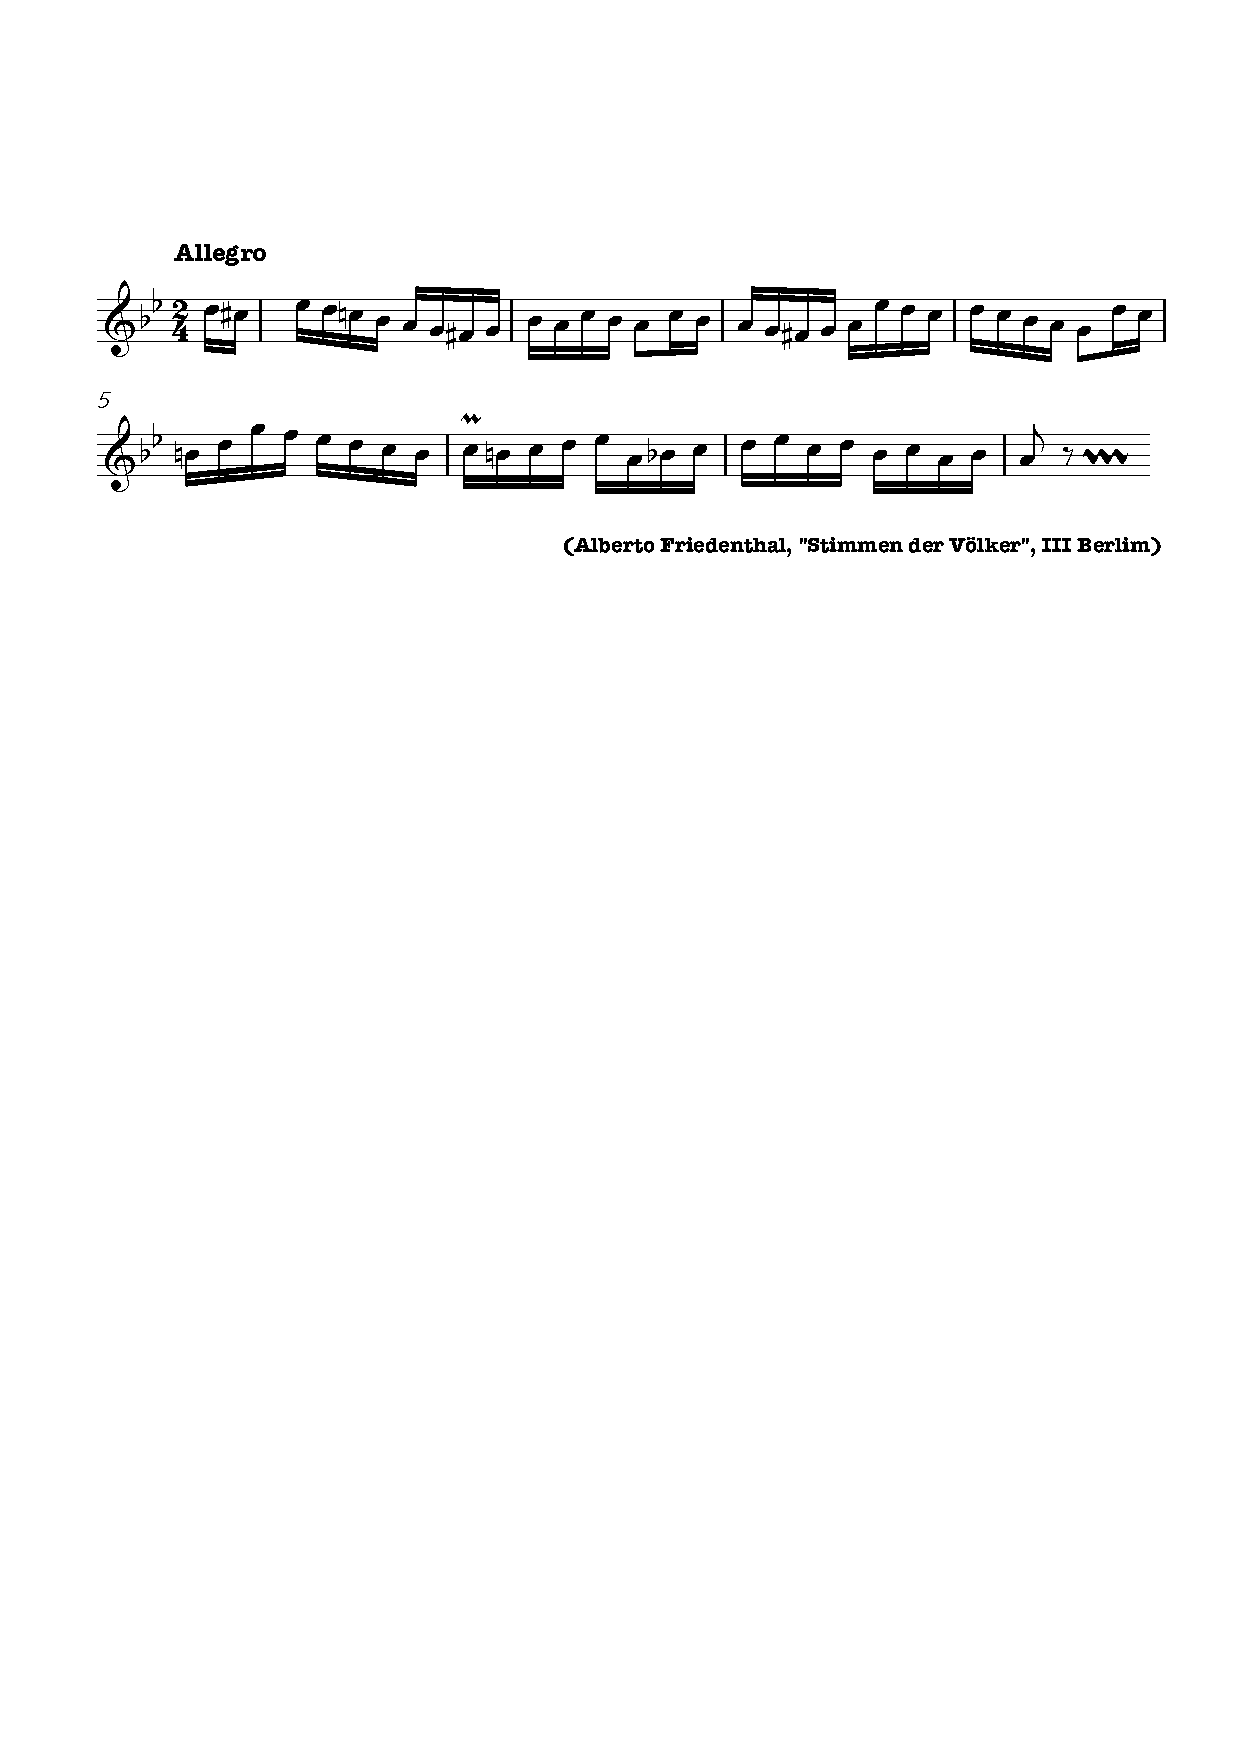
\includegraphics[width=\textwidth]{./imgs/fig4.pdf}
 \end{figure}

Na realidade, foi de uma complexa mistura de elementos estranhos que se
formou a nossa música popular. E não dei todos. A modinha, ao contato da
valsa europeia, modificou-se profundamente. Hoje em dia bom número das
modinhas populares são em três por quatro e valsas legítimas. A polca, a
mazurca, a \textit{schottish} se tornaram manifestação normal da dança
brasileira. A modinha algumas vezes se reveste do corte rítmico da
chotis. Nos fandangos \textit{bailados} dos caipiras paulistas de Cananeia
(mais distintos que os \textit{batidos}, em que existe bate-pé e bate-mão),
me informaram que, sob outros títulos, subsistem ainda a figuração
coreográfica da valsa (\textit{rocambole}, \textit{chamarrita}), da polca (\textit{dandão}), da
mazurca (\textit{faxineira}). Às vezes em nosso canto passam acentos nórdicos,
suecos, noruegueses\ldots{} Como que vieram parar aqui? Acentos idênticos
também se encontram em Portugal e principalmente Espanha.

Às vezes um canto nosso é\ldots{} russo duma vez. Outras vezes é um canto
russo que, mudando as palavras, todos tomariam por brasileiro. Se
observe a brasilidade enorme desta versão do canto ``Troyka'', me dada
pelo pintor russo Lasar Segall:

 \begin{figure}[H]
 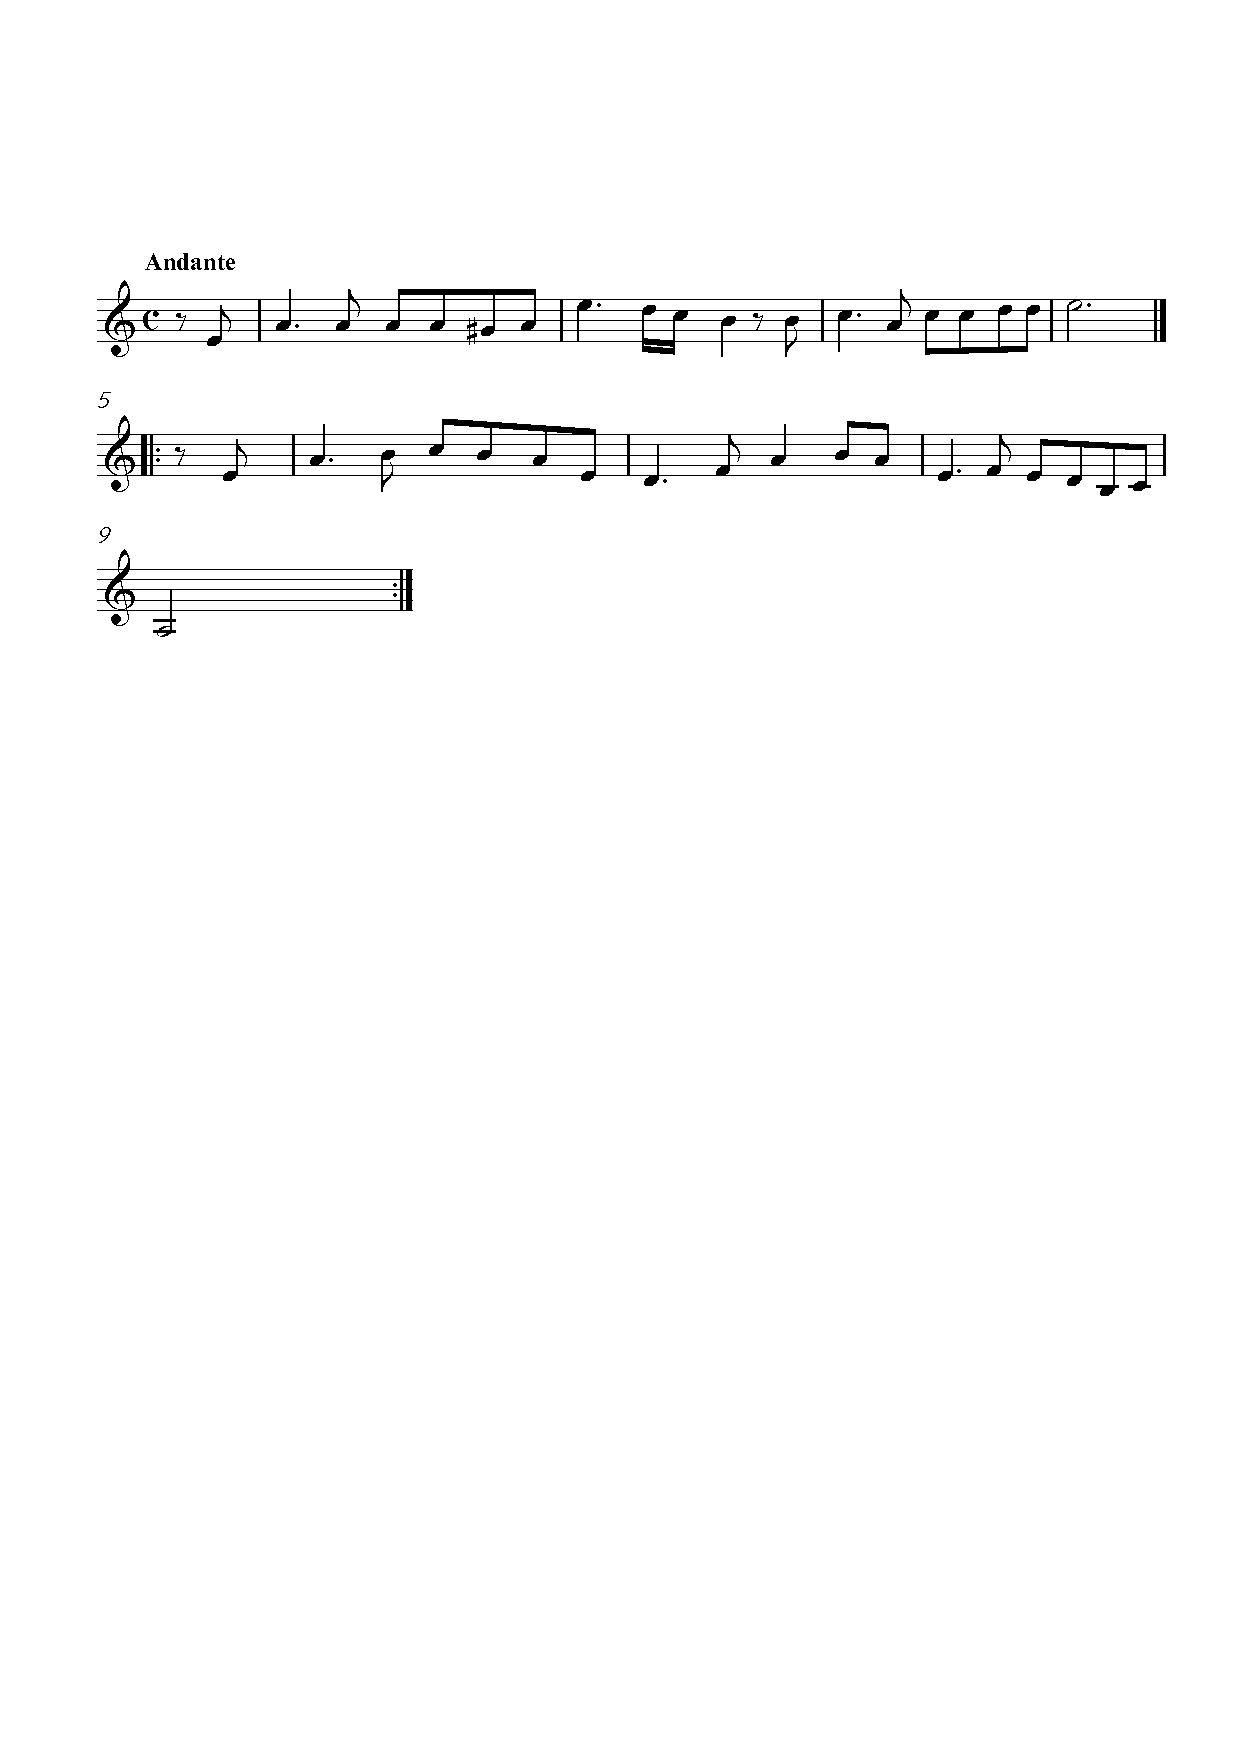
\includegraphics[width=\textwidth]{./imgs/fig5.pdf}
 \end{figure}

Tantas e mais influências vinham e vêm ainda ornar a nossa raça
nascente. Raça também muito misturada, o certo é que demonstrava desde
logo forte musicalidade. Grande número de viajantes estranhos atestaram
a propensão do brasileiro para a música. Von Weech afirma que \textit{a
musicalidade é inata no povo} (do Brasil); e lamenta a nossa ignorância
e leviandade, que não nos deixa completar estudos musicais sérios e nos
leva a fazer música \textit{quase como os canários}. Saint-Hilaire,
assistindo em Minas uma ópera composta e representada por brasileiros,
comenta que \textit{não tem nada de extraordinário a gente esbarrar com
músicos no Brasil, pois qualquer vila os possui}. Schlichthorst,
comentando a psicologia do penetra de assustados, no Rio de Janeiro, diz
que a especialidade dele é \textit{possuir talento musical} --- o que o torna
logo tratado por todos na palminha das mãos. E reconhecendo embora que
não havia então, no país, virtuoses excepcionais, verificava que \textit{todos
os brasileiros sem exceção gostam da música}. Martius também comentando
jocosamente em 1817 uma representação em São Paulo da opereta ``Le
déserteur'' (provavelmente a ópera cômica de Monsigny?) por mulatos e
pretos, afirma em seguida que guarda \textit{opinião muito favorável sobre o
talento musical dos paulistas}. E seguem assim os viajantes, unânimes
em louvar a musicalidade do brasileiro. Essa musicalidade é real; porém,
até agora deu melhores frutos no seio do povo inculto que na música
erudita. Muito mal nos está fazendo a falta de cultura tradicional, a
preguiça em estudar, a petulância mestiça com que os brasileiros, quer
filhos de algo, filhos de bandeirantes ou de senhores de engenhos, quer
vindos proximamente de italianos, de espanhóis, de alemães, de judeus
russos, se consideram logo gênios insolúveis, por qualquer habilidade de
canário que a terra do Brasil lhes deu. Nos consola é ver o povo inculto
criando aqui uma música nativa que está entre as mais belas e mais
ricas.

Pois colhendo elementos alheios, triturando-os na subconsciência
nacional, digerindo-os, amoldando-os, deformando-os, se fecundando, a
música popular brasileira viveu todo o século \textsc{xix}, bem pouco étnica
ainda. Mas no último quarto do século principiam aparecendo com mais
frequência produções já dotadas de fatalidade racial. E, no trabalho da
expressão original e representativa, não careceu nem cinquenta anos:
adquiriu caráter, criou formas e processos típicos. Manifestação duma
raça muito variada ainda como psicologia, a nossa música popular é
variadíssima. Tão variada que às vezes desconcerta quem a estuda. As
formas principais que emprega são: na lírica a moda, a toada, e o
romance, de caráter rural; a modinha e o lundu, no geral de caráter
urbano. Na dança: o maxixe, fixado no Rio de Janeiro no último quarto do
século \textsc{xix}; o cateretê; a valsa; o samba, ou baiano, como é chamado
atualmente no Nordeste. Na dança-dramática se distingue o bumba meu boi
(Nordeste) ou boi-bumbá (Amazônia) em que as fadigas do pastoreio se
transformaram em arte, celebrando ritualmente a morte e ressurreição do
boi. Subsistem ainda, bem generalizados no país, os congos e os
congados, bem como, da Bahia para o Norte especialmente, os bailados de
vário nome popular, que celebraram as lutas de cristãos e mouros, e os
trabalhos do mar. E pela importância que podem ter, resta citar entre as
danças-dramáticas, os reisados de Natal, os cabocolinhos e os maracatus
carnavalescos. Uma forma de canto social importante é o coco, existente
em todo o Nordeste, utilizando sistematicamente o processo responsorial,
solo e coro. Quase sempre dançando.

Os instrumentos da preferência popular são: fora da cidade, a viola, a
sanfona, o ganzá, a puíta; na cidade o violão, a flauta, o oficleide, a
clarineta e ultimamente o saxofone, por influência do jazz, além da
percussão. Possuímos agrupamentos orquestrais típicos. Alguns já
registrei no meu ``Ensaio'' citado. Luciano Gallet registra como
agrupamento característico das serestas e choros cariocas a composição:
clarineta, oficleide, flauta, trombone, cavaquinho, bateria. Nos bois
nordestinos o acompanhamento tradicional é rebeca e viola. Nos cocos só
aparece a percussão, representada pela puíta, o munganguê, o reco-reco e
o ganzá.

Choros, serestas, são nomes genéricos aplicados a tudo quanto é
música noturna de caráter popular, especialmente quando realizada ao
relento. O choro implica no geral participação de pequena orquestra com
um instrumento mais ou menos solista, predominando sobre o conjunto.

Uma fonte importante da música popular é a feitiçaria, com suas
cerimônias em que o canto e a dança dominam. Nos cultos de direta origem
africana (candomblé, macumba, xangô) até hoje se consegue recolher
música originalíssima como caráter, que, sem ser legitimamente africana,
foge bastante das nossas constâncias melódicas populares. Também no
catimbó nordestino, numerosos cantos são de notável originalidade de
caráter, sem que nos seja possível atribuir a qualquer tradição
ameríndia, base de inspiração desse culto, essa originalidade musical.

As manifestações popularescas que tiveram maior e mais geral
desenvolvimento são, desde o século passado, as modinhas, os maxixes e
sambas urbanos que andam profusamente impressos. No século \textsc{xix}
distinguiram-se mais como inventores de modinhas, Xisto Bahia, que era
também ator, Mussurunga, Almeida Cunha, Carlos Dias da Silva, Soares
Barbosa. Nos maxixes, salientaram-se duas figuras valiosas: Ernesto
Nazaré, fixador do maxixe de caráter carioca, e Marcelo Tupinambá que
deu a essa dança uma expressão mais geral, entre cabocla e praceana.
Especializaram-se ainda Donga, Sinhô e Noel Rosa, as figuras
contemporâneas mais interessantes do samba impresso. Menção especial
deve ser feita a Francisca Gonzaga, tipo curioso de compositora cujas
danças e cantigas, muitas dotadas de caráter brasileiro forte, mereciam
maior atenção e respeito aqui. A atividade musical dela é tipicamente
oitocentista. Figuram com destaque entre os nossos compositores de
operetas e revistas do Segundo Império: Henrique Alves de Mesquita,
Ábdon Milanez, F.\,Alvarenga, Cardoso de Menezes. Entre os cantadores
contemporâneos corre a fama de Manuel do Riachão, nordestino diz que
invencível no desafio. Catulo Cearense, tipo rastaquera de nordestino
\textit{carioquizado}, gênio sem eira nem beira, tanto na modinha como
especialmente na toada e também no romance, inventou algumas das mais
admiráveis criações da poesia cantada popularesca.



\chapter{Dicionário musical brasileiro\footnote{Mário de Andrade compilou neste dicionário os principais termos da música brasileira, com todos os vocábulos próprios e características históricas curiosas. Conferir \textit{Dicionário musical brasileiro}, Ministério da Cultura, 1989.}}

\paragraph{Canção} (\textit{s.\,f.}) Composição em verso. Na \textit{Pequena
história da música}, Mário de Andrade analisa a canção europeia: ``O
século \textsc{xvi} é a fase da canção. Porém agora o que se entende por canção não
é uma toada de gênero popular, nem se inventou ainda a mania de imitar
\textit{popularescamente} o povo. Trata-se duma forma desenvolvida e aprimorada,
um pouco amaneirada mesmo, como poesia. Poeticamente há grande variedade
na forma de estrofes, cada estrofe em geral seguida por estribilho. O
tamanho das canções também varia muito, e se algumas são pequeninas,
outras não acabam mais, de tamanhas. Seus temas preferidos são o
amor\ldots{} e o amor. Em geral o amor. Porém amor cortês, cheio de
delicadezas e \textit{grã-finismo} de expressão. Às vezes se canta a natureza
também.

Musicalmente a canção é sistematicamente tratada, por todo o século,
em polifonia que vai de duas até seis vozes. Em todo caso, dentro dessa
concepção polifônica, o \textit{madrigal} itálico, a \textit{chanson} francesa, a \textit{song}
inglesa, o \textit{lied} alemão, trazem o germe da melodia acompanhada. Tanto o
sentido individualista dos textos, como a evolução cada vez mais
harmônica da polifonia, propunham, desde já, o canto solista acompanhado
por instrumento. E a canção avassala a criação artística do tempo. Assim
como o século anterior fora a fase da missa, o século \textsc{xvi} é a fase da
canção. Se os artistas, ainda até o século \textsc{xviii} escreverão muita música
religiosa, o que os particulariza e define o espírito novo é a música
profana. %(ä. ed.\,p.\,66). (\textsc{dm})

% V.tb.: 200, vol.\,\textsc{ii}, p.\,129; 204, p.\,33; 388, p.\,99; 499, p.\,153; 569,
% s.p.; \textsc{lira}, M. Música Popular Brasileira, Jornal do Brasil, \textsc{rj}., 13 fev.
% 1938.

\paragraph{Lundu} (\textit{s.\,m.}) Canto e dança populares no Brasil durante o século
\textsc{xviii}, introduzidos provavelmente pelos escravos de Angola, em compasso
2/\,4 onde o primeiro tempo é frequentemente sincopado. No início era uma
dança cuja coreografia foi descrita como tendo certa influência
espanhola pelo alteamento dos braços e estalar dos dedos semelhante ao
uso de castanholas tendo, no entanto, a umbigada característica. A
coreografia foi aproximada por alguns autores às do samba e do
batuque.

O \textit{lundu canção} foi conhecido durante o primeiro Império e, no século \textsc{xix},
depois de ter frequentado os salões familiares, caiu em desuso. A falta
de documentos antigos dificulta a caracterização do lundu como forma; as
peças encontradas apontam como traço comum o emprego da síncopa.

O acompanhamento do canto e da dança, que era feito por instrumentos de
cordas dedilhadas, foi substituído, no salões, pelo piano. %(\textsc{dm-ma})

Era conhecido em Portugal desde o século \textsc{xvi} e aí condenado.\footnote{Braga, J.,
\textit{História da poesia popular}, vol.\,2, 1902, p.\,445.} Nessa mesma obra
citada,\footnote{Na página 447.} vem que Stafford na sua \textit{History of Music} de 1830,
dava como cantos nacionais portugueses e lundus e as modinhas. Teófilo
Braga\footnote{Op. cit., p.\,484.} mostra que Tolentino fala na existência dum
\textit{lundum chorado} bem suave. A expressão ``lundu chorado'' corre também
no Brasil. Numa paródia à ``Judia'' de Tomás Ribeiro, feita por
Antônio Lopes Cardoso em 1870 na Bahia, vem a estrofe:

\begin{quote}
\small{
Dorme! --- eu descanto a regalar-te o ouvido
Com o sustenido desta voz nasal!
Dorme e não ouça o lundu chorado
de quem torrado não possui real.}\footnote{Querino,
M. \textit{A Bahia de outr'ora}, 1922, p.\,122.} %(\textsc{ma})}
\end{quote}

Também o cronista pernambucano Lopes Gama fala na existência praceana,
pela segunda metade do século \textsc{xviii}, do lundu chorado ``que se dançava às
umbigadas ao som da cítara e viola''.\footnote{Costa, F., \textit{Folclore pernambucano},
\textsc{rihgb}, 1908, p.\,221.}

Um escritor português do século \textsc{xix}\footnote{Op. cit., p.\,22, sem nomear.}
discrimina entre os lundus dançados em Portugal por importação do
Brasil, o lundu chorado e o lundu do Rio. %(\textsc{ma})

Dum trecho pernambucano de 1809, citado em Pereira da Costa: ``Sobressaía a toda essa penitente chusma um duende, sob a forma de demônio, ou diabo em carne, o qual dançando continuamente o
\textit{desonestíssimo} lundu com todas as mutanças da mais lúbrica torpeza,
acometia com mingadas (\textit{umbigadas}) a todos indistintamente.''\footnote{Op. cit.,
p.\,200.}

Também de lundu fala o Conde de Pavolide, Dão José da Cunha Grã Ataíde e
Melo, atribuindo a \textit{brancos e pardos} e não o achando tão censurável
assim ao passo que reprovava formalmente e procurara destruir os
``bailes {[}\ldots{}{]} que os pretos da Costa da Mina fazem às escondidas ou em
casas ou roças com uma preta mestra, com altar de ídolos etc.''\footnote{Op. cit., p.\,204.} %(\textsc{ma})

Em 1838, Lopes Gamas descreveu: ``sempre debaixo do compasso do mais
rigoroso lundu, entravam pela igreja e ali, postas em redor de tal
bandeira, saracoteavam as ancas, reboleavam-se, davam umbigadas, puxavam
fieira''.\footnote{Op. cit., p.\,195.}

Nina Rodrigues descrevendo o lundu em 1895 ainda o cita como uma ``dança
de pretos, muito indecente, na qual se faz mil espécies de movimento com
o corpo.'' Afirmando que, na lavagem do Bonfim, na quinta-feira
antecedente à festa, os pretos cantavam lundus e cantos de feitiçaria a
Obalatá dentro da igreja.\footnote{\textit{L'animisme fetichiste des nègres de
Bahia}, 1900, p.\,142.} %(\textsc{ma})

Ao publicar a melodia de um lundu nordestino no \textit{Ensaio sobre
música brasileira},\footnote{1972, p.\,142.} Mário de Andrade acrescenta: 

\begin{quote}
\small{A palavra \textit{lundu} está desaparecendo. Aqui no centro do país indica
especialmente uma cantiga praceana de andamento mais vivo que o da
modinha e com texto de caráter cômico, irônico, indiscreto. O
\textit{Gosto da negra} que se segue, corresponde bem ao que chamamos por
aqui de lundu. No Norte lundu ainda permanece uma dança, me informa o
prof.\,José Domingos Brandão, de Belém, autor de duas \textit{Rapsódias
brasileiras pra orquestra}.}
\end{quote}

%\\[2\baselineskip]IMAGENS

% TEXTO DA IMAGEM: ``Eu gosto da negra/ Cor de carvão/ Eu tenho por ela/
% Grande paixão// Que bem m'importa/ que falem de mim/ Eu gosto da negra/
% Mesmo assim''

Além destas canções, Mário de Andrade
trabalha em 1928 com o ``Lundu do escravo'', colhido em
Araraquara, na \textit{Revista de Antropofagia}, em artigo que depois
figurará em \textit{Música, doce música}. Na coletânea \textit{Modinhas
imperiais}, de 1930, inclui um lundu para piano. Quatro lundus colhidos
no Nordeste foram por ele destinados a \textit{Na pancada do ganzá}.\footnote{\textit{As melodias do boi e outras peças}, org. Oneyda Alvarenga, 1987,
p.\,131--135. Dentre estes, o intitulado ``Corujinha'' mereceu um
verbete à parte.} %(V.\,``Corujinha'' %(\textsc{dm})

\textit{Enlevou-se em lundus}, frase feita expressiva da insinuação que levou
alguém a um determinado ato em Turquel (Portugal).\footnote{Ribeiro, J.,
``Linguagem popular de Turquel'', Rev. \textit{Lusitana}, 28 (¼); 156, 1930).}
%(\textsc{ma})

A palavra ainda foi registrada com as seguintes grafias: \textit{landum}, \textit{londum}
e \textit{lundum}.\footnote{\textsc{almeida}, R. \textit{História da música brasileira}, 1942, p.\,72-78;
\textsc{carvalho}, P. \textit{História do fado}, 1903, p.\,5; \textsc{mendonça}, R. \textit{A influência
africana no português do Brasil}, 1935, p.\,210; \textsc{rodrigues}, J. \textit{Os africanos
no Brasil}. 1932, p.\,265.}
%(\textsc{dm})
% Ver também: ``Lundu chorado''.

\paragraph{Marcha} (\textit{s.\,f.}) Gênero de composição caracterizado pela escrita
em compasso binário, ou mais raramente quaternário, com o primeiro tempo
fortemente acentuado, principalmente instrumental. No Brasil a marcha
popularizou-se nos blocos carnavalescos como marcha-rancho e marcha de
salão e segue a fórmula introdução instrumental e estrofe-refrão.

Renato Almeida salienta que não só no Brasil a marcha passou de
acompanhamento de passos militares a dança, citando o musicólogo Hugo
Riemann que aproxima o gênero à \textit{polonaise} e à \textit{intrada}.\footnote{\textsc{almeida}, R. \textit{História da música brasileira}, 1942, p.\,193.}
%Ver também: ``Marcheta''.
%(\textsc{dm})
%(\textsc{dm-ma}).

\paragraph{Maxixe} (\textit{s.\,m.}) Dança e canto populares em voga no Brasil a
partir do século passado. ``Foi da fusão da habanera, pela rítmica, e da
polca, pela andadura, com a adaptação da síncopa afro-lusitana que
originou-se o maxixe''.\footnote{Andrade, Mário de. Ernesto Nazaré. \textit{Música,
doce música}, 1976, p.\,125.}\footnote{Nota da pesquisa: Acolhemos para este termo documentação de Mário de Andrade aqui selecionada e organizada segundo: origens do termo, dança e canto, análise rítmico-melódica; influências estrangeiras; a evolução do gênero.}


\paragraph{Origens do termo, dança e canto} O maxixe foi pela primeira vez dançado no palco em 4 de fevereiro de 1876, na paródia de Artur Azevedo \textit{A filha de Maria Angu}, \textit{à
La Fille de Mime Angot.}

Foi levado à cena do Phoenix Dramático. Tinha por assunto a questão do
livro a ação começava na Praça do Mercado, entre quitandeiros. Aparecia
no quadro intitulado ``Legume'', de que falava Chiquinha Gonzaga. A
protagonista foi Rosa Villiot, era a Clarinha Angu. A atriz Delmary
fazia o papel de Chica Valsa e o ator Silva o de Angelo Bitu. Não há
referência ao ator que teria feito o papel de maxixe, pois, com certeza
era papel bem secundário. A crítica não se refere a ele.\footnote{\textit{Revista
Ilustrada}, 5 de fevereiro de 1876.}

Observações: é provável que fosse o ator que na peça fez o papel de
maxixe quem dançasse no baile de carnaval dos Estudantes de Heidelberg.
Talvez pelo local e pela natureza do baile, ele o tivesse feito com tal
exagero que tivesse despertado a atenção e atraído imitadores. Pela data
da representação da peça o carnaval estaria próximo.\footnote{``Comunicação
feita ao professor Mário de Andrade por Mariza Lira''. Datiloscrito,
papel ofício sem assinatura.}

Villa (Lobos) descobriu, julga ter descoberto a origem do maxixe. Um
afinador da Casa Arthur Napoleão que tem 84 anos e um certo Comendador
de igual idade assistiram ao nascimento do maxixe num clube
carnavalesco, o primeiro que se fundou no Rio. \textit{Maxixe} era o apelido do
sujeito que nesse clube dançou o lundu de um certo jeito particular que
imitado depois por outros deu no maxixe. A música de lundu evoluiu da
mesma forma, impulsionada pelo movimento rítmico da dança. Os dois
velhos conhecem o primeiro \textit{lundu-maxixe}. Villa tomou nota de tudo. Será mesmo
assim? Pelo menos é razoável.

O Clube parece que se chama Altenberg ou coisa parecida.\footnote{Bandeira,
Manuel. Trecho de carta a Mário de Andrade. Manuscrito, sem indicações
de local, data e assinatura, in: \textit{Dic. mus. brasileiro}, \textsc{ieb-usp}.}

A versão do Villa sobre o aparecimento do maxixe se pode aceitar. O
caso é possível. Se você arranjasse um jeito de controlar o caso, as
duas opiniões concordantes sobre o aparecimento do maxixe seriam
suficientes pra gente dar como certa a versão. A tal sociedade
carnavalesca de que você fala qual é, são os Estudantes de Heildelberg
e creio mesmo que tenho ou no Melo Morais Filhos, ou num artigo na
\textit{Kosmus}, a data em que essa sociedade existiu.\footnote{Andrade, Mário de.
\textit{Cartas a Manuel Bandeira}, 1958, p.\,147, 10 out. 1926.}

Os Estudantes e Heidelberg são dali por volta de 1879, 80.

Um tal de Américo Fluminense na Kosmos de fevereiro de 1907 fez uma
barafunda medonha e diz que de aí por 1878 apareceu a Sociedade Bohème e
em seguida os Estudantes; afirma mais adiante que nesse mesmo 1878 só
restavam em campo os Fenianos, Tenentes e os Democráticos. Memo Morais
Filho, outro leviano, confessa no entanto não poder precisar de datas,
porém do escrito dele se depreende que é nessa década de 1870 a 1880 que as
Sociedades antigas viveram com esplendor. Isso concorda com as
informações que tive, pois os informantes, um deles ao menos, que tem
agora 84 anos, estaria na sensual e festeira casa dos trinta --- \textit{Ora
o Cruz Perigo de Nazareth}, que deve ser da última década do século \textsc{xix}
(princípio ou menos por 1889) já a melodia é bem menos nossa e o ritmo
acompanhante traz a síncopa do primeiro tempo (segunda e terceira partes) que viria a
dar na constância rítmica do acompanhamento do maxixe. %(\textsc{m.a}).

\begin{quote}
\small{Encontrei uma referência ao maxixe (a mais antiga que conheço) num
folhetim do ator Vasques, de 24 de janeiro de 1884, na \textit{Gazeta da Tarde}, na qual
se vê que a dança desse nome já era conhecida, mas se dançava ao som de
uma polca-tango. Será que ainda não haveria a música característica, que
realmente fusiona aqueles dois elementos? A indicação desse folhetim,
encontrei --- sem data --- no livro do Procópio sobre o Vasques e, depois,
na Biblioteca Nacional, identifiquei a citação e a data.}\footnote{Almeida,
Renato. \textit{Carta a Mário de Andrade}, 26 jul, 1941, in:
Dic.mus.brasileiro, \textsc{ieb-usp}.}
\end{quote}

\begin{quote}
\small{Só uma vez encontrei neles (os \textit{Folhetins}, de França Júnior) a
palavra (maxixe), no sentido de festa caseira, sinônimo de forrobodó e
chinfrim: `não há habitação modesta onde no dia seguinte ao de um
\textit{forrobodó}, \textit{maxixe}, ou \textit{chinfrim}, como se diz na
gíria, não se veja a dona de casa a mandar a negrinha empastar de barro
as manchas de gordura que sujam o soalho''. {[}\ldots{}{]} Tenho um amigo de perto
de 70 anos que chegou ao Rio em 1885 onde já encontrou o maxixe. Sendo os
\textit{Folhetins} de 1876, pode-se concluir que a dança e o nome nasceram dentro
daquela década.}\footnote{Manuel Bandeira, \textit{O sonho de França Júnior}, Bol. de
Ariel, 4: 16, 1934}
\end{quote}

É muito importante que o Dicionário de Baurepaire-Rohan de 1889 já dá o
maxixe como espécie de batuque, no Rio Grande do Sul. Em tão pouco tempo
teria ido pra lá e se popularizado assim! %(\textsc{ma})

\textit{A Semana} (Campinas), n.\,16 de junho de 1894, noticiando a
representação da revista \textit{O Itararé} falava que ``a música é leve e
agradável, apenas lhe notamos o abuso (!) dos tangos e lundus''. Era bem
o maxixe como música esses tangos de então, mas o nome, como Nazareth
conservaria toda a vida pros seus maxixes, era ainda tango. Mas o n.\,14 de julho seguinte da mesma revista, elogiando a atividade da casa
editora Vieira Machado e \textsc{c}., diz que esta não limitava a nossa atividade
a imprimir ``quanta música banal venha à cabeça dos nossos fazedores de
quadrilhas, polcas e valsas.''

De maxixe, de tango, nem pio. Aliás, nem de lundu também. Mas é porque
este não se dança talvez\ldots{}%(\textsc{ma})

Em 1907 já estava definitivamente introduzido na alta sociedade
brasileira, pois num baile oferecido ao ex-presidente argentino Julio
Roca o maxixe se dançou.\footnote{V.\,Rossi, \textit{Cosas de negros}, 1926, p.\,179}

Etimologia fantasista. Entre os incas tem uma febre acompanhada de
tremores e mexidos de corpo, chamada \textit{chuchu}. Chuchu = maxixo. Maxixo =
maxixe. %(\textsc{ma})

\smallskip

--- Vamos dançar a dança do fulano.

\smallskip

E de tanto dizerem a \textit{dança do maxixe}, veio por facilitação a falarem
só no \textit{maxixe}, da mesma forma que o \textit{gallopavo} achado no México pela
expedição de Hernando Cortez, denominado pelos nossos cronistas
(Gandavo, Fernão Cardin) \textit{galo do Peru}, se veio a falar só em \textit{peru}. %(\textsc{ma})

Essa mistura de religiosidade, sensualidade, política, etc. que se
encontra nas letras de certas cantigas dançadas, dos maxixes em geral
provém talvez do caráter impovisatório dessas letras? Talvez. Odum e
Johnson no seu livro deles \textit{The Negro and his Songs} observam que
\textit{many songs owe their origins to the negro´s keeness at improvisation.}
Ora, o maxixe pelo coreograficamente parece ter sido uma improvisação.
(Informação do Villa).\footnote{Odum, Howard W. e Johnson, Guy
B. 1925, p.\,153.} %(\textsc{ma})

Ausência de religiosidade cristã se exprimindo musicalmente entre nossos
negros. Não temos os \textit{spirituals} dos negros norte-americanos. Porém a
religiosidade misturada se mostra em certos maxixes e é certo que então
os santos do cristianismo dotados dos nomes mais estrambólicos se
misturam com nomes de antigos deuses africanos. Assim, num recente maxixe
de Donga, se misturam Xangô, que não pode ser senão o Shango, deus do
trovão entre os iorubás que, sabemos, vieram escravos em grande número pra
cá, e Ogum. Ora, este Ogum, segundo explicação de negros, é São Jorge. %(\textsc{ma}).

A própria coincidência tradicional de ser a época de carnaval a
escolhida pro lançamento de maxixes novos que irão servir pro gasto do
ano parece provar que o maxixe é eminentemente carnavalesco e proveio do
carnaval. %(\textsc{ma})

\paragraph{Análise rítmico-melódica} Reparar que as antecipações de finais de frases, fazendo-as terminar
antes da parte lógica do tempo forte em que teoricamente deviam cair,
fenômeno que só duns cinco anos pra cá principiou a se manifestar na música
de dança impressa e de que o Souto parece ser o primeiro (tem o
\textit{Bem-te-vi} do Pernambuco), reparar que já aparece em milongas
clássicas montevideanas, como \textit{La canaria de canelones} e
\textit{Pejerrey con papas}.\footnote{Rossi V., \textit{Cosas de negros}, 1926,
p.\,393 e 394. Exemplos 1 e 2; ver p.\,306-307.} Talvez a necessidade
fisiológica da síncopa nos tenha levado a essa admirável originalidade
rítmica, a todos nós descendentes de negros e vivendo no novo mundo.
(Uma coisa importante a observar é o emprego síncopa pelos negros
africanos que não saíram da África. Empregam-na?) --- Reparar nas milongas
todas citadas em Cosas de negros a tercina característica do 1º tempo,
coisa que viria entre nós dar na síncopa. Ora esta síncopa no compasso
de 2/\,4 do maxixe, do tango, da milonga é perfeitamente mais fácil que a
tercina que trazia dois ritmos diferentes em polifonia. Seria talvez uma
evolução forçada e ignara da tercina? Ou esta uma forçada transposição
erudita daquela? Outros tantos problemas que só a pesquisa de arquivos
possa elucidar.

\paragraph{A evolução do gênero maxixe-samba} Evolução do maxixe pro samba contemporâneo, parece mais uma reação do negrismo étnico do brasileiro contra o branquismo excessivo do maxixe.
Notar que, este, quer pelo maxixe carioca (\textit{lignée} Nazareth) quer
pelo maxixe estaduano-caipira (\textit{lignée} Tupinambá) apresentava quer
pela dureza às vezes excessiva da síncopa (ver maxixes Tamoio e Benga
que tenho num disco Victor), quer principalmente pela linha melódica,
excessivamente branca, pra não dizer, imediatamente europeia (como na
maioria dos tangos de Nazareth), excessivo caráter e força europeia. O
samba contemporâneo, pela sua maior languidez, diluição de síncopa, pelo
seu muito maior dengue rítmico, pelo seu movimento menos duro e
andamento um bocado mais nazarento, pelo entrecortado da sua linha
melódica cheia de paradas no canto, pela sua volta à dança sempre vocal
(o maxixe era muitas vezes exclusivamente instrumental), pela nova
\textit{timbração} vocal mais efeminada (ambas estas, timbre vocal e frascado
entrecortado, influências do jazz e do blues ianques), é uma reação negra
contra o maxixe, é uma volta a nascentes mais idôneas, é uma
reprimitivização de nossa dança urbana, por direta influência negra, ou
de caracteres negros assimilados por brancos.\footnote{Discografia: Disco Victor n.\,33.318. Lado \textsc{a} -- \textsc{cardoso}, Carlos.
\textit{Tamoyo}; Maxixe. Orchestra Victor brasileira. Lado \textsc{b} -- \textsc{souza},
s.p. de \textit{\textsc{benga}}: Maxixe, Idem.}\footnote{Bibl.: \textsc{almeida}, R. \textit{História da música brasileira}, 1942, p.\,189;
\textsc{andrade}, M. ``\textit{Chiquinha Gonzaga}'', Música, doce música, 1976,
p.\,329-333; \textsc{idem} -- ``Ernesto Nazaré'', \textit{Ibidem}, p.\,121-130; \textsc{idem}.
``Ernesto Nazareth'', \textit{Ibidem} p.\,319-323; \textsc{idem} ``Influência portuguesa
nas rodas infantis do Brasil'', \textit{Ibidem}, p.\,85; \textsc{idem}. Originalidade
do maxixe. \textit{Ilustração Musical\ldots{}} ano 1, nº2, set, 1930, p.\,45;
\textsc{fluminense}, A. \textit{O Carnaval no Rio}, Kosmos, 4: s.p, 1907;
\textsc{friedenthal}, \textit{A. Musik, Tanz und -- Dichtung bei den Kreolen
Amerikas}, 1913, p.\,297; \textsc{lira}, Mariza. \textit{Carta a Mário de Andrade},
Rio de Janeiro, 6 mar. 1940, manuscrito tinta, in: Documentação sobre
maxixe, \textit{Dicionário musical Brasieliro} -- \textsc{ieb-usp}.}
%Ver também: ``Passo''.
%(\textsc{dm})
%(\textsc{ma})

\paragraph{Modinha} (\textit{s.\,f.}) Canto de salão, urbano, conhecido no Brasil e
em Portugal, com versos ``a maioria das vezes anônimos. {[}\ldots{}{]} Mas às
vezes os poetas bons também eram musicados. Sem insistir sobre o caso
famoso do mulato Caldas Barbosa cuja modinhação contumaz se tornou de
citação obrigada pelo muito que fez babar de gozo os reinóis, pode-se
dizer que desde os mestres da Escola Mineira até fins do romantismo,
todos os nossos poetas ilustres foram melodizados em modinhas. Dos
grandes nomes românticos os mais aproveitados foram Gonçalves Dias,
Álvares de Azevedo e Casimiro de Abreu. {[}\ldots{}{]} Quanto à música importa
desde logo salientar um problema curioso e ainda não tratado. E que
aliás importa diretamente às origens da modinha. Os documentos e textos
mais antigos se referindo a ela já designam peças de salão e todos
concordam em dar à modinha uma origem erudita, ou pelo menos da
semicultura burguesa. Melo Morais Filho a fixa como ``descendente em
linha reta da melodia italiana'',\footnote{\textit{Serenatas e saraus}, vol.\,3, p.\,\textsc{xi}.} a sra.\,Wodehouse também, e Friedenthal reconhece em algumas delas
parecença extrema com Mozart.''\footnote{Andrade, M. de. \textit{Modinhas
imperiais}, 1980, p.\,6.}

\begin{quote}
\small{A modinha se originou só do formulário melódico europeu. A sensualidade
mole, a doçura, a banalidade que lhe é própria (e que também coincidia
com um estado de espírito e de arte universal no tempo, como já
indiquei) só lhe pôde provir da geografia, do clima, da alimentação. E
prova disso é que a ela se adaptavam muito bem os estrangeiros parando
aqui.}\footnote{Andrade, M. de., op. cit., p.\,7.}
\end{quote}

Para Mário de Andrade, ``a palavra \textit{moda} pra designar canção vernácula
corre desde muito em Portugal.'' Segundo ele, é ``jeito luso-brasileiro
acarinhar tudo com diminutivos. A palavra \textit{modinha} nasceu assim. E assim
viveu, esporádica, em todos os meios luso-brasileiros até que
precisou-se dum termo pra designar as canções de salão em língua materna
e música setecentista. Chamaram-lhe \textit{modinhas} por serem delicadas. Ou por
terem se tornado eruditamente mais curtas, sem aquela complacência com o
tempo que o povo tem nas suas manifestações artísticas. E a palavra, de
\textit{modinha}, qualificativo acarinhante, passou a \textit{modinha}, uma forma.''

Forma ou gênero? Mais propriamente gênero, gênero de romanças de salão
em vernáculo, um tempo, e já agora, um dos gêneros da cantiga popular
urbana.

Porque de fato as modinhas imperiais tomaram muitas das formas da ária
\textit{sete-e-oitocentista}. As possuímos em duas estrofes \textsc{a}--\textsc{b} em duas
estrofes e refrão \textsc{a}--\textsc{b}--\textsc{c}; em estrofe e refrão \textsc{a}--\textsc{c}; em duas estrofes e um \textit{stretto} que faz as vezes de refrão \textsc{a}--\textsc{b}--\textsc{d}; e mesmo algumas eruditíssimas, vestindo o espartilho da \textit{Ária de Capo}, como é o
caso de \textit{A conha e a virgem}, de José Amat e mais poucas.

\begin{quote}
\small{Na divisão rítmica as modinhas variam também bastante, as mais antigas
no geral preferindo os cortes binários do \textsc{c} ou do 2/\,4; as já
influenciadas pelo cantabile italiano e pela valsa, no período da
decadência indo frequentemente dos compassos compostos ao pleno 3/4 em
que mais elas se vulgarizariam no povo. A maioria das nossas modinhas
populares atuais, e não as melhores, valisticamente reprisam a
ternaridade. Em todo caso o binário da \textit{schottisch}, que o gosto romântico
pelo exótico pôs em moda justamente um século faz, entra em boa
concorrência com as modinhas-valsas. E isto já parece de pura adaptação
popular, pois ao passo que na documentação impressa do Segundo Império
as modinhas em 3/\,4 abundam que é um desespero, não conheço nenhum
documento de então seguindo a rítmica da \textit{schottisch}.}\footnote{Andrade, M. de,
op.cit., p.\,8--9.}
\end{quote}

Mário de Andrade, analisando as tonalidades de modinhas por ele
coligidas, conclui que nelas ``há uma certa preferência pelo menor'',
algumas iniciando no modo maior e concluindo no menor. ``O mais
impressionante nesse processo maior-menor é que não se trata de tons
relativos, como já falei. Ninguém passa de fá maior para ré menor e
vice-versa. A tonalidade persevera sempre a mesma na maioria dos casos.
{[}\ldots{}{]} Também muito rara é a modulação pra dominante. {[}\ldots{}{]} Mais uma
tendência que se repete bem, muito mais que o transporte à dominante,
{[}\ldots{}{]} Mais uma tendência que se repete bem, muito mais que o transporta
à dominante, é a modulação pra quarto grau. {[}\ldots{}{]} O que não pode se
contestar na verificação destas constâncias --- e por isso me demorei
tanto nelas --- passagem de maior pra menor dentro da mesma tonalidade,
modulação prá subdominante --- é que nos compositores vivos, tão
justamente desejosos de se nacionalizar, podiam tirar daí verdadeiros
planos tonais que especificaram de jeito característico a maneira
modulatória nacional.''\footnote{Andrade, M, de. op.cit. p.\,11.}\footnote{Nota da pesquisa: Mário de Andrade colheu vasta documentação
complementar à coletânea Modinhas imperiais (1930). Selecionamos, a
seguir, notas e bibliografia que acrescentam dados ao estudo por ele
publicado. Como texto se pode bem perceber que as modinhas devem ter desde muito
uma vida nacional. Nos bailes pastoris mais natigos, nas óperas do
``Judeu'', a todo momento, os textos de árias, são como forma, temas e
sabor, absolutamente sementalhas às modinhas do Primeiro Império.}

Guilherme de Melo\footnote{\textit{A música no Brasil}, 1908, p.\,146.} sem citar abonação
nenhuma (e naturalmente se autorizando das afirmativas do perigoso
Teófilo Braga sem quem se estriba por demais) afirma que já no século \textsc{xvi}
a ``canção romântica (ele quer dizer sentimental) transportando-se de
Portugal para o Brasil com o título de modinha, nome derivado de mote ou
moda, estaciona-se entre nós até o fim do século \textsc{xviii}, quando sob a
influência das açafatas brasileiras de d.\,Maria \textsc{i} transportando-se de
novo para Portugal, torna-se o gênero de música mais predileto nas
distrações do passo''. Acervo de verdades e afirmativas levianas. Onde a
abonação do título modinha já existente no século \textsc{xvi}. Principalmente já
não como diminutivo apenas de moda, mas caracterizando um, senão uma
forma, pelo menos um gênero de canções em língua portuguesa? Além disso:
que hipótese mais fácil essa da modinha se conservar estacionária e
recôndita, até florescer viva nos fins do século \textsc{xviii}!\ldots{} E se é verdade
que as açafas brasileiras de d.\,Maria, cantavam ao paço as modinhas de
cá, elas foram apenas um dos muitos elementos que contribuíram para
divulgação da nossa modinha em Portugal e dentro do próprio paço. O
sucesso de Lereno (Caldas Barbosa), a volta à terrinha dos portugueses
``brasileiros'', os navegantes, os nobres e administradores portugueses
repatriados, os escravos (que nem mais tarde a negra brasileira cantando
romances tradicionais a Garret) eram outros tantos elementos que levaram
pra Portugal todas as forças vivas e valores estimáveis da colônia.
Dentre estes a modinha estava. E com efeito, como em seguida Guilherme
de Melo vem citando todo um sonho de hipóteses de Teófilo Braga
explicando a modinha brasileira pelo fenômeno de sobrevivência arcaica
da tradição nas colônias distantes. Se isso é possível (e seguem esta
hipótese um terno de afirmações erradas) não subsiste dado nenhum que
permita uma verificação de ordem objetiva e científica. A palavra
\textit{modinha} muito provavelmente foi usada primeiro em Portugal. Isso não
tem importância nenhuma. Da segunda metade do século \textsc{xviii} em diante até
quase o fim do século passado existiram modinhas portuguesas e
brasileiras de salão. Essas são no geral muito descaracterizadas como
expressão étnica. Podem ser às vezes bonitas; como significação racial
são água-morna, coisa que não vai nem vem. O serem lânguidas, o serem
sensuais, como tendência geral não é suficiente pra caracterizá-las
etnicamente. Modinhas brasileiras e portuguesas de salão, desses tempos,
se confundem. Estão crivadas da melódica açucarada e bamba comum aos
compositores europeus de segunda ordem, que pululavam em França, Itália,
Alemanha nos tempos da \textit{ópera comique}, da decadência da \textit{ópera buffa};
das árias e romances inda bem românticos, e da melodia água doce dos
Noturnos, dos romances sem palavras, dos \textit{morceaux de salon}, e peças
características timbrando em sentimentalismo. Porém, ao lado dessas
modinhas de são, brasileiras e portuguesas, o que reivindica a modinha
como propriedade nossa é que ao passo que o povo português fixava a sua
canção amorosa especialmente urbana no fado, o povo brasileiro estava
criando, mais necessária, mais racial, uma modinha bem diferente da de
salão e nela fixou a sua canção amorosa especialmente praceana.

Apesar de muitos fados cantados no Brasil e dos muitos compostos aqui, o
fado é português. Não funciona em nossa vida nacional. Apesar de vinda,
como palavra, de Portugal, apesar de todas as modinhas portuguesas, a
modinha é brasileira. Não funciona na vida nacional dos portugueses %(\textsc{ma})

Na verdade as origens da modinha são confusas. Se como palavra ela vem
diretamente de moda, já palavra musical portuguesa, se como forma e
caráter as mais antigas modinhas portuguesas e brasileiras ficadas, se
confundem, são todas \textit{de salão} e demonstram mais ou menos uma sempre
evidente influência geral europeia e erudita: há no entanto um argumento
que depõe muito a favor duma origem brasileira da modinha. (Dou o
argumento, mas sempre repetindo que isso não é que decide sobre a
realidade brasileira da modinha). Não há exemplo duma forma musical
erudita a forma musical popular, ter, como forma, se popularizado. Pelo
contrário, quase todas as formas eruditas encontram mais ou menos a sua
base no populário. As mais antigas modinhas registradas em publicações
especializadas ou em viajantes, todas elas demonstram pouquíssimos ou
nenhum caráter popular. Todas elas apresentam versos evidentemente
eruditos ou de direta influência erudita, e música de caráter
sintomaticamente erudito europeu. Ora, desde os fins do século \textsc{xviii} quem
quer que se refira a modinhas em Portugal, fala sempre cantigas \textit{de
salão}, ouvidas em salão e tocadas por \textit{gente fina}. Ao passo que os que
se referem a modinha brasileira existida no Brasil, já às vezes falam
que ela está no domínio do povo e não apenas da gente de salão (provar
isso com documentação). E de fato imemorialmente, pelo menos desde fins
do século \textsc{xviii}, quando a palavra modinha aparece se referindo a uma forma
especial de canção em língua portuguesa, imemorialmente a modinha é do
domínio da gente popular do Brasil, ao passo que como forma jamais em
Portugal, não se popularizou. Não sendo crível que uma forma erudita
tenha neste caso se popularizado, é muito mais evidenciável que a forma
da modinha nascendo e vivendo no povo colonial do Brasil, tenha sido
colhida do povo por amadores refinados ou gozadores apenas e desse então
transportada pros salões e aí tivesse por deformação erudita adquirido
da forma que apresentam as modinhas \textit{de salão} daqueles tempos. Pode
ser mesmo que nem tenha havido esse transporte da rua pro salão, mas que
a um canto erudito de fundo e forma fundamentalmente europeus, porém já
na língua vernácula, a gente \textit{de salão}, compositores amadores, tenham
dado o mesmo nome duma forma popular, só pelo encanto invejável desta e
a coincidência de língua usada. E assim a ária de salão sem batismo, se
tornou modinha, usurpando a individualidade já com nome duma criação
popular. E acresce ainda que em Portugal se falou e muito nas modinhas
brasileiras ao passo que no Brasil jamais em modinhas portuguesas %(\textsc{ma})

Ao falar na evolução da palavra modinha, vinda de moda apenas por
diminutivo acariciante que acabou de ficando como gênero definido de
canção, dizer que essa transição semântica do termo se surpreende bem o
caipira paulista Zico Dias,\footnote{Disco Victor 33395.} cantador de modas, a
que chama de fato \textit{modas} mas que nas palavras das modas desse disco,
fala que \textit{ao cantar esta modinha}. O mesmo fenômeno semântico surpreende
entre os caipiras com que privei uma semana na barranca do mojo\footnote{Disco Victor 33395: lado \textsc{a} -- \textsc{dias}, Zico e Ferrinho. \textit{Revolução
Getúlio Vargas}: moda de viola. Zico Dias e Ferrinho com viola. Lado \textsc{b} --
idem. \textit{A Morte de João Pessoa}.}

%(\textsc{ma})

Notar que em nossas dias mesmo estamos possivelmente assistindo à
fixação duma palavra assim, com o designativo de \textit{marchinha} dado às
danças marchas de carnaval. Ninguém dirá \textit{marcha carnavalesca} o que
apenas poderá ter outro sentido. Pra designar essas músicas que a gente
dança com o \textit{passo} nos bailes e ruas de carnaval, só se usará a palavra
\textit{marchinha}.\footnote{Veja capa disco n.\,333.} %(\textsc{ma})

Disco Victor 33951 (n.\,\textsc{m.\,a.} 333): lado \textsc{a} -- \textsc{martins}, Roberto e Silva, Walfrido. \textit{Morena que dorme na rede: samba-canção}. Floriano Belham com o grupo do Canhoto. Lado \textsc{b} -- \textsc{alves}, Ataulfo. \textit{Saudades do meu barracão}. 
%Idem. Nota \textsc{ma}:

\begin{quote}
\small{
Modinha -- À medida que esta desaparece ou
vive mais desatendida dos seresteiros, vai sendo porém substituída pelo
samba-canção, que é realmente uma modinha nova, de caráter novo, mas
canção lírica solista, apenas com um rítmica fixa de samba, em que porém
a agógica já não é mais realmente coreográfica, mas de canção lírica.
Ora isso é evolução lógica, por assim dizer, fata. A modinha de salão
passada pra boca do povo popular adotou mesmo ritmos coreográficos, o da
valsa e o da chótis principalmente. Ora estes eram sempre ritmos
importados, não da criação imediata nacional. O samba-canção é a
nacionalização definitiva da modinha.}
\end{quote}

Um mestiço Alexandre, aluno do cabeleireiro Frederico Reis que estava
instalado no Largo do Rocio, além de cabeleireiro, se distinguia por um
talento vocal de imitação extraordinário. Era sopranista, possuindo uma
voz mista, de soprano e contralto com que imitava a Charton e a
Casaloni, cantando o Trovador, com tal perfeição de enganar. Foi por
isso apelidado Alexandre Trovador. E como cabeleireiro e cantador ia na
melhor roda da Corte, e aí cantava modinhas de Efreu, José Maurício,
Noronha, Mazziotti, Fachinetti, as mais difíceis, e também trechos de
óperas que ele mesmo acompanhava ao violão. %(\textsc{ma}).

%(\textsc{dm-ma})

%Ver também: \textit{Gaturna, mote}.

% V.tb.: \textsc{braga}, J. \textit{História da poesia popular portuguesa}, v.2,
% 1905, p.437, 476 e 557, 35, p. \textsc{xvi}; 37, p503; 49, p6; 74, p.12; 120,
% v.1, p.67, 136, v.2, p.181, 172, p.31, 191, v.2, ´.32, 197, v.6, p.28,
% 199, v.1, p.306, 200, v.1, p.234, 219, p.24; 227. p;155; 240, v1, p.258,
% v.2, p.348;258, p.137; 282, p.238 e 241; 297, p. 130; 299, p.16, 336,
% ´.137; 339; 340; p.\textsc{xxiv}; 344, p102, 471, p 187; 501, p. 41; 502, p 69;
% 550, p.147; 566, p.63; 597; p.612, p126; 702; p.130; 728; p.405; 768;
% p.162 e 169.


% \chapter{Bibliografia de Mário de Andrade}

% \textit{Ensaio sobre a música brasileira} (vol. \textsc{vi} das Obras Completas)

% \textit{Aspectos da música brasileira} (vol. \textsc{xi} das Obras Completas)

% \textit{Pequena história da música}, 1944. (Vol. \textsc{viii} das Obras Completas)

% \textit{O baile das quatro artes}. (Vol. \textsc{xiv} das Obras Completas)

% \textit{Dicionário musical brasileiro} (compilação e organização de Oneyda
% Alvarenga e Flávio Camargo Toni

% \textit{A Música Popular Brasileira na vitrola de Mário de Andrade}. Org.
% Flávia Camargo Toni. São Paulo: Editora \textsc{senac sp}, 2004.



%\backmatter

%Cronologia
%Índice remissivo
	%Glossário de verbetes
	%Indíce biográfico
	%Índice de referências multinormativas
	%Glossário mitológico, histórico e geográfico

% Indice remissivo (package: `\usepackage{makeidx}` e no início do arquivi `\makeindex`
% \printindex

% Indice
% \renewcommand{\contentsname}{Índice}
% \setcounter{tocdepth}{3}
% \tableofcontents

% \endnotes

%\input{Y-publicidade}	   % [lista de livros publicados]
\pagebreak

\ifodd\thepage\blankpage\fi

\parindent=0pt
\footnotesize\thispagestyle{empty}

%\noindent\textbf{Dados Internacionais de Catalogação na Publicação -- CIP}\\
%\noindent\textbf{(Câmara Brasileira do Livro, SP, Brasil)}\\

%\dotfill\\

% \hspace{20pt}ISBN 978-65-86238-31-0 (Livro do Estudante)

% \hspace{20pt}ISBN 978-65-86238-30-3 (Manual do Professor)\\[6pt]

% \hspace{20pt}\parbox{190pt}{1. Crônicas Brasileira. 2. Contos Brasileiro. 3. Rosa, Alexandre. I. Título.}\\[6pt]

% \hspace{188pt}\textsc{cdd}-B869.8

%\dotfill

%\noindent{}Elaborado por Regina Célia Paiva da Silva CRB -- 1051\\
\mbox{}\vfill


\begin{center}
		\begin{minipage}{.75\textwidth}\tiny\noindent{}
		\centering\tiny
		Adverte-se aos curiosos que se imprimiu este 
		livro na gráfica Meta Brasil, 
		em \today, em papel pólen soft, em tipologia MinionPro e Formular, 
		com diversos sofwares livres, 
		entre eles \LaTeX \& git. \ifdef{\RevisionInfo{}}{\par(v.\,\RevisionInfo)}{}\medskip\\\
		\adforn{64}
		\end{minipage}
\end{center}		   % [colofon]



\checkandfixthelayout
\end{document}
